\documentclass[leqno,fleqn,12pt,titlepage]{amsbook}
\usepackage{fullpage}
\usepackage{subfigure}
\usepackage{amsmath}
\usepackage{amsthm}
\usepackage{amssymb}
\usepackage{graphicx}
\usepackage{subfigure}
\usepackage{mdwlist}
\usepackage[small,bf]{caption}
\usepackage{calc}
\usepackage{float}
\usepackage{setspace} 
\usepackage{rotating}
\usepackage{verbatim}
\usepackage{textcomp}
\usepackage[pdftitle={Linear Programming Lecture Notes},
colorlinks=true,linkcolor=black,urlcolor=blue,citecolor=red]{hyperref}
\interdisplaylinepenalty=2500

%%FIX List of Figures Problem
\makeatletter
\renewcommand\l@figure{\@tocline{0}{3pt plus2pt}{0pt}{3.3em}{}}
\makeatother

%%UNCOMMENT FOR iPad notes
%\makeatletter
%\renewcommand*\@ptsize{4}
%\let\small\relax
%\let\footnotesize\relax
%\let\scriptsize\relax
%\let\tiny\relax
%\let\large\relax
%\let\Large\relax
%\let\LARGE\relax
%\let\huge\relax
%\let\Huge\relax
%\input{size1\@ptsize.clo}
%\makeatother

%\renewcommand{\thefigure}{\thechapter.\arabic{figure}}
\numberwithin{equation}{chapter}
\numberwithin{figure}{chapter}

\floatstyle{boxed}
\newfloat{cgalgorithm}{thp}{lop}
\floatname{cgalgorithm}{Algorithm}
\newenvironment{algorithm}
{\begin{cgalgorithm}[htbp]\small}
{\normalsize\end{cgalgorithm}}

%\doublespace



\title{Linear Programming: Penn State Math 484 Lecture Notes\\
		{\small Version 1.8.3}\\
		}
\author{
	Christopher Griffin\\
	\textcopyleft~2009-2014\\
	\vspace*{1em}
	{\scriptsize Licensed under a 
	\href{http://creativecommons.org/licenses/by-nc-sa/3.0/us/}
	{Creative Commons Attribution-Noncommercial-Share Alike 3.0 United States License}}
	\\
	{\small \textit{With Contributions By:}\\
	Bob Pakzad-Hurson\\ Greg Ference\\ Veselka Kafedzhieva\\ Michael Cline\\
	Akinwale Akinbiyi\\Ethan Wright\\
	Richard Benjamin\\
	Douglas Mercer\\}
	
	
}
\date{}

\newtheorem{theorem}{Theorem}[chapter]
\newtheorem{proposition}[theorem]{Proposition}
\newtheorem{lemma}[theorem]{Lemma}
\newtheorem{corollary}[theorem]{Corollary}

\theoremstyle{definition}
\newtheorem{definition}[theorem]{Definition}

\theoremstyle{remark}
\newtheorem{remark}[theorem]{Remark}
\newtheorem{example}[theorem]{Example}
\newtheorem{exercise}{Exercise}

\begin{document}
\frontmatter


\maketitle
\tableofcontents

\listoffigures


\chapter*{Preface}
This is a set of lecture notes. It is not a book. You should probably go away and come back when you have a real textbook on Linear Programming. Okay, do you have a book? Alright, let's move on then. This is a set of lecture notes for Math 484--Penn State's undergraduate Linear Programming course. Since I use these notes while I teach, there may be typographical errors that I noticed in class, but did not fix in the notes. If you see a typo, send me an e-mail and I'll add an acknowledgement. There may be many typos, that's why you should have a real textbook.

The lecture notes are (roughly) based on the first 6 chapters of Bazaraa et al.'s \textit{Linear Programming and Network Flows} book. This is a reasonably good book, written primarily by and for Industrial Engineers. The only problem I have with the book is that it does not present major results in the standard \textit{theorem-proof} style common to mathematical discourse. This set of notes corrects this problem by presenting the material in a format for presentation to a mathematics class. Many of the proofs in this set of notes are adapted from the textbook with some minor additions. (For example, each time Bazaraa et al. ask, ``Why?'' in a proof, I provide this information.) Additionally, I prefer to present maximization problems, while \textit{Linear Programming and Network Flows} prefers the minimization format. I've modified all the proofs to operate on maximization problems. When used with the book, the student can obtain a complete set of proofs for elementary Linear Programming.

In order to use these notes successfully, you should have taken courses in:
\begin{enumerate*}
\item Vector calculus (Math 230/231 at Penn State)
\item Matrix algebra (Math 220 at Penn State)
\end{enumerate*}
I review a substantial amount of the material you will need, but it's always good to have covered prerequisites before you get to a class. That being said, I hope you enjoy using these notes!
\mainmatter
\chapter{Introduction to Optimization}
Linear Programming is a sub-field of optimization theory, which is itself a sub-field of Applied Mathematics. Applied Mathematics is a very general area of study that could arguably encompass half of the engineering disciplines--if you feel like getting into an argument with an engineer. Put simply, applied mathematics is all about applying mathematical techniques to understand or do something practical. 

Optimization is an exciting sub-discipline within applied mathematics! Optimization is all about making things better; this could mean helping a company make better decisions to maximize profit; helping a factory make products with less environmental impact; or helping a zoologist improve the diet of an animal. When we talk about optimization, we often use terms like \textit{better} or \textit{improvement}. It's important to remember that words like better can mean \textit{more of something} (as in the case of profit) or \textit{less of something} as in the case of waste. As we study linear programming, we'll quantify these terms in a mathematically precise way. For the time being, let's agree that when we optimize something we are trying to make some decisions that will make it better.

\begin{example}
Let's recall a simple optimization problem from differential calculus (Math 140): Goats are an environmentally friendly and inexpensive way to control a lawn when there are lots of rocks or lots of hills. (Seriously, both Google and some U.S. Navy bases use goats on rocky hills instead of paying lawn mowers!) 

Suppose I wish to build a pen to keep some goats. I have 100 meters of fencing and I wish to build the pen in a rectangle with the largest possible area. How long should the sides of the rectangle be? In this case, making the pen \textit{better} means making it have the largest possible area.

The problem is illustrated in Figure \ref{fig:GoatPen}.
\begin{figure}[htbp]
\centering
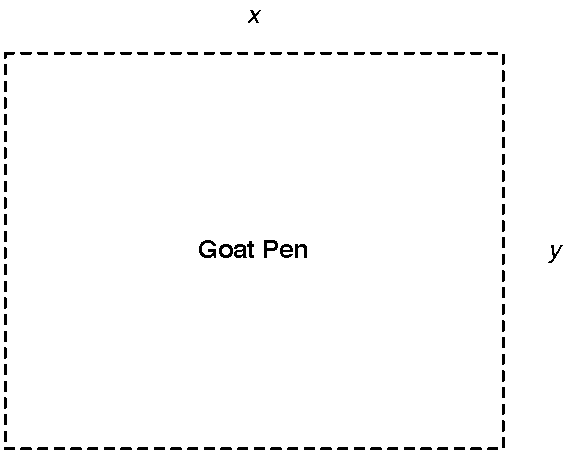
\includegraphics[scale=0.6]{GoatPen.pdf}
\caption{Goat pen with unknown side lengths. The objective is to identify the values of $x$ and $y$ that maximize the area of the pen (and thus the number of goats that can be kept).}
\label{fig:GoatPen}
\end{figure}
Clearly, we know that:
\begin{equation}
2x + 2y = 100
\label{eqn:GoatPerimeter}
\end{equation}
because $2x + 2y$ is the perimeter of the pen and I have 100 meters of fencing to build my pen. The area of the pen is $A(x,y) = xy$. We can use Equation \ref{eqn:GoatPerimeter} to solve for $x$ in terms of $y$. Thus we have:
\begin{equation}
y = 50 - x
\end{equation}
and $A(x) = x(50-x)$. To maximize $A(x)$, recall we take the first derivative of $A(x)$ with respect to $x$, set this derivative to zero and solve for $x$:
\begin{equation}
\frac{dA}{dx} = 50-2x = 0;
\end{equation}
Thus, $x = 25$ and $y = 50-x = 25$. We further recall from basic calculus how to confirm that this is a maximum; note:
\begin{equation}
\left.\frac{d^2A}{dx^2}\right|_{x = 25} = -2 < 0
\end{equation}
Which implies that $x = 25$ is a \textit{local maximum} for this function. Another way of seeing this is to note that $A(x) = 50x-x^2$ is an ``upside-down'' parabola. As we could have guessed, a square will maximize the area available for holding goats. 
\label{ex:GoatExample}
\end{example}

\begin{exercise} A canning company is producing canned corn for the holidays. They have determined that each family prefers to purchase their corn in units of 12 fluid ounces. Assuming that metal costs 1 cent per square inch and 1 fluid ounce is about 1.8 cubic inches, compute the ideal height and radius for a can of corn assuming that cost is to be minimized. [Hint: Suppose that our can has radius $r$ and height $h$. The formula for the surface area of a can is $2\pi r h + 2 \pi r^2$. Since metal is priced by the square inch, the cost is a function of the surface area. The volume of the can is $\pi r ^2 h$ and is constrained. Use the same trick we did in the example to find the values of $r$ and $h$ that minimize cost.
\label{exer:Can}
\end{exercise}

\section{A General Maximization Formulation}
Let's take a more general look at the goat pen example. The area function is a mapping from $\mathbb{R}^2$ to $\mathbb{R}$, written $A : \mathbb{R}^2 \rightarrow \mathbb{R}$. The domain of $A$ is the two dimensional space $\mathbb{R}^2$ and its range is $\mathbb{R}$.

Our objective in Example \ref{ex:GoatExample} is to maximize the function $A$ by choosing values for $x$ and $y$. In optimization theory, the function we are trying to maximize (or minimize) is called the \textit{objective function}. In general, an objective function is a mapping $z: D \subseteq \mathbb{R}^n \rightarrow \mathbb{R}$. Here $D$ is the domain of the function $z$. 

\begin{definition} Let $z: D \subseteq \mathbb{R}^n \rightarrow \mathbb{R}$. The point $\mathbf{x}^*$ is a \textit{global maximum} for $z$ if for all $\mathbf{x} \in D$, $z(\mathbf{x}^*) \geq z(\mathbf{x})$. 
A point $\mathbf{x}^* \in D$ is a \textit{local maximum} for $z$ if there is a neighborhood $S \subseteq D$ of  $\mathbf{x}^*$  (i.e., $\mathbf{x}^* \in S$) so that for all $\mathbf{x} \in S$, $z(\mathbf{x}^*) \geq z(\mathbf{x})$. 
\label{defn:Max}
\end{definition}

\begin{remark} Clearly Definition \ref{defn:Max} is valid only for domains and functions where the concept of a neighborhood is defined and understood. In general, $S$ must be a topologically connected set (as it is in a neighborhood in $\mathbb{R}^n$) in order for this definition to be used or at least we must be able to define the concept of \textit{neighborhood} on the set\footnote{Thanks to Bob Pakzad-Hurson who suggested this remark for versions after 1.1.}.
\end{remark}

\begin{exercise} Using analogous reasoning write a definition for a global and local minimum. [Hint: Think about what a minimum means and find the correct direction for the $\geq$ sign in the definition above.]
\end{exercise}

In Example \ref{ex:GoatExample}, we are constrained in our choice of $x$ and $y$ by the fact that $2x + 2y = 100$. This is called a \textit{constraint} of the optimization problem. More specifically, it's called an \textit{equality constraint}. If we did not need to use all the fencing, then we could write the constraint as $2x + 2y \leq 100$, which is called an \textit{inequality constraint}. In complex optimization problems, we can have many constraints. The set of all points in $\mathbb{R}^n$ for which the constraints are true is called the \textit{feasible set} (or feasible region). Our problem is to \textit{decide} the best values of $x$ and $y$ to maximize the area $A(x,y)$. The variables $x$ and $y$ are called \textit{decision variables}. 

Let $z:D\subseteq\mathbb{R}^n \rightarrow \mathbb{R}$; for $i=1,\dots,m$, $g_i:D\subseteq\mathbb{R}^n \rightarrow \mathbb{R}$; and for $j=1,\dots,l$ $h_j:D\subseteq\mathbb{R}^n \rightarrow \mathbb{R}$ be functions. Then the general maximization problem with objective function $z(x_1,\dots,x_n)$ and \textit{inequality constraints} $g_i(x_1,\dots,x_n) \leq b_i$ ($i=1,\dots,m$) and \textit{equality constraints} $h_j(x_1,\dots,x_n) = r_j$ is written as:
\begin{equation}
\left\{
\begin{aligned}
\max\;\;& z(x_1,\dots,x_n)\\
s.t.\;\;& g_1(x_1,\dots,x_n) \leq b_1\\
& \hspace*{0.5in}\vdots\\
& g_m(x_1,\dots,x_n) \leq b_m\\
& h_1(x_1,\dots,x_n) = r_1\\
&\hspace*{0.5in}\vdots\\
&h_l(x_1,\dots,x_n) = r_l
\end{aligned}
\right.
\label{eqn:GeneralMax}
\end{equation}
Expression \ref{eqn:GeneralMax} is also called a \textit{mathematical programming problem}. Naturally when constraints are involved we define the global and local maxima for the objective function $z(x_1,\dots,x_n)$ in terms of the feasible region instead of the entire domain of $z$, since we are only concerned with values of $x_1,\dots,x_n$ that satisfy our constraints.

\begin{example}[Continuation of Example \ref{ex:GoatExample}] We can re-write the problem in Example \ref{ex:GoatExample}:
\begin{equation}
\left\{
\begin{aligned}
\max \;\; & A(x,y) = x y \\
s.t. \;\; & 2x + 2y = 100\\
& x \geq 0\\
& y \geq 0 
\end{aligned}\right.
\label{eqn:GoatMax}
\end{equation}
Note we've added two inequality constraints $x \geq 0$ and $y \geq 0$ because it doesn't really make any sense to have negative lengths. We can re-write these constraints as $-x \leq 0$ and $-y \leq 0$ where $g_1(x,y) = -x$ and $g_2(x,y) = -y$ to make Expression \ref{eqn:GoatMax} look like Expression \ref{eqn:GeneralMax}.
\end{example}

We have formulated the general \textit{maximization} problem in Proble \ref{eqn:GeneralMax}. Suppose that we are interested in finding a value that minimizes an objective function $z(x_1,\dots,x_n)$ subject to certain constraints. Then we can write Problem \ref{eqn:GeneralMax} replacing $\max$ with $\min$. 

\begin{exercise} Write the problem from Exercise \ref{exer:Can} as a general minimization problem. Add any appropriate non-negativity constraints. [Hint: You must change $\max$ to $\min$.] 
\end{exercise}

An alternative way of dealing with minimization is to transform a minimization problem into a maximization problem. If we want to minimize $z(x_1,\dots,x_n)$, we can maximize $-z(x_1,\dots,x_n)$. In maximizing the negation of the objective function, we are actually finding a value that minimizes $z(x_1,\dots,x_n)$.

\begin{exercise} Prove the following statement:
\textit{Consider Problem \ref{eqn:GeneralMax} with the objective function $z(x_1,\dots,x_n)$ replaced by $-z(x_1,\dots,x_n)$. Then the solution to this new problem minimizes $z(x_1,\dots,x_n)$ subject to the constraints of Problem \ref{eqn:GeneralMax}.}[Hint: Use the definition of global maximum and a multiplication by $-1$. Be careful with the direction of the inequality when you multiply by $-1$.]
\label{exer:MinForMax}
\end{exercise}
%\begin{proof} Let $(x_1^*,\dots,x_n^*)$ maximize $-z(x_1,\dots,x_n)$ subject to the constraints of Problem \ref{eqn:GeneralMax}. Then for all other $(x_1,\dots,x_n)$ satisfying the constraints of Problem \ref{eqn:GeneralMax} we have: 
%\begin{displaymath}
%-z(x_1^*,\dots,x_n^*) \geq -z(x_1^*,\dots,x_n^*)
%\end{displaymath}
%Multiplying by $-1$ on both sides yields:
%\begin{displaymath}
%z(x_1^*,\dots,x_n^*) \leq z(x_1^*,\dots,x_n^*)
%\end{displaymath}
%and this holds for all other $(x_1,\dots,x_n)$ satisfying the constraints of Problem \ref{eqn:GeneralMax}. Thus $(x_1^*,\dots,x_n^*)$ is a solution to the problem of minimizing $z(x_1,\dots,x_n)$ subject to the constraints of Problem \ref{eqn:GeneralMax}. 
%\end{proof} 

\section{Some Geometry for Optimization}
A critical part of optimization theory is understanding the geometry of Euclidean space. To that end, we're going to review some critical concepts from Vector Calculus (Math 230/231). I'll assume that you remember some basic definitions like \textit{partial derivative} and \textit{Euclidean space}. If you need a refresher, you might want to consult \cite{MT03, Stew07}. 

We'll denote vectors in $\mathbb{R}^n$ in boldface. So $\mathbf{x} \in \mathbb{R}^n$ is an n-dimensional vector and we have $\mathbf{x} = (x_1,\dots,x_n)$. %It's common to associate an $n$-dimensional vectors with a $1 \times n$ matrix(row vector) or an $n \times 1$ matrix (column vector). 
\begin{definition}[Dot Product]
Recall that if $\mathbf{x}, \mathbf{y} \in \mathbb{R}^n$ are two $n$-dimensional vectors, then the \textit{dot product} (\textit{scalar product}) is:
\begin{equation}
\mathbf{x} \cdot \mathbf{y} = \sum_{i=1}^{n} x_i y_i
\end{equation}
where $x_i$ is the $i^\text{th}$ component of the vector $\mathbf{x}$. 
\end{definition}

An alternative and useful definition for the dot product is given by the following formula. Let $\theta$ be the angle between the vectors $\mathbf{x}$ and $\mathbf{y}$. Then the dot product of $\mathbf{x}$ and $\mathbf{y}$ may be alternatively written as:
\begin{equation}
\mathbf{x}\cdot\mathbf{y} = ||\mathbf{x}||||\mathbf{y}||\cos\theta
\end{equation}
This fact can be proved using the \textit{law of cosines} from trigonometry. As a result, we have the following small lemma (which is proved as Theorem 1 of \cite{MT03}):
\begin{lemma} Let $\mathbf{x}, \mathbf{y} \in \mathbb{R}^n$. Then the following hold:
\begin{enumerate*}
\item  The angle between $\mathbf{x}$ and $\mathbf{y}$ is less than $\pi/2$ (i.e., acute) iff $\mathbf{x}\cdot\mathbf{y} > 0$. 
\item The angle between $\mathbf{x}$ and $\mathbf{y}$ is exactly $\pi/2$ (i.e., the vectors are orthogonal) iff $\mathbf{x}\cdot\mathbf{y} = 0$. 
\item The angle between $\mathbf{x}$ and $\mathbf{y}$ is greater than $\pi/2$ (i.e., obtuse) iff $\mathbf{x}\cdot\mathbf{y} < 0$.
\end{enumerate*}
\end{lemma}

\begin{exercise} Use the value of the cosine function and the fact that $\mathbf{x}\cdot\mathbf{y} = ||\mathbf{x}||||\mathbf{y}||\cos\theta$ to prove the lemma. [Hint: For what values of $\theta$ is $\cos\theta > 0$.]
\end{exercise}

\begin{definition}[Graph] Let $z:D \subseteq \mathbb{R}^n \rightarrow \mathbb{R}$ be function, then the \textit{graph} of $z$ is the set of $n+1$ tuples:
\begin{equation}
\{(\mathbf{x},z(\mathbf{x})) \in \mathbb{R}^{n+1} | \mathbf{x} \in D\}
\end{equation}
\label{def:Graph}
\end{definition}
When $z: D \subseteq \mathbb{R} \rightarrow \mathbb{R}$, the graph is precisely what you'd expect. It's the set of pairs $(x,y) \in \mathbb{R}^2$ so that $y = z(x)$. This is the graph that you learned about back in Algebra 1.  

\begin{definition}[Level Set] Let $z:\mathbb{R}^n \rightarrow \mathbb{R}$ be a function and let $c \in \mathbb{R}$. Then the \textit{level set of value $c$ for function $z$} is the set:
\begin{equation}
\{\mathbf{x}=(x_1,\dots,x_n) \in \mathbb{R}^n | z(\mathbf{x}) = c\} \subseteq \mathbb{R}^n
\end{equation} 
\label{def:LevelSet}
\end{definition}

\begin{example} Consider the function $z = x^2 + y^2$. The level set of $z$ at $4$ is the set of points $(x,y) \in \mathbb{R}^2$ such that:
\begin{equation}
x^2 + y^2 = 4
\end{equation}
You will recognize this as the equation for a circle with radius 4. We illustrate this in the following two figures. Figure \ref{fig:LevelSet3D} shows the level sets of $z$ as they sit on the 3D plot of the function, while Figure \ref{fig:LevelSet2D} shows the level sets of $z$ in $\mathbb{R}^2$. The plot in Figure \ref{fig:LevelSet2D} is called a \textit{contour plot}. 
\begin{figure}[ht]
\centering
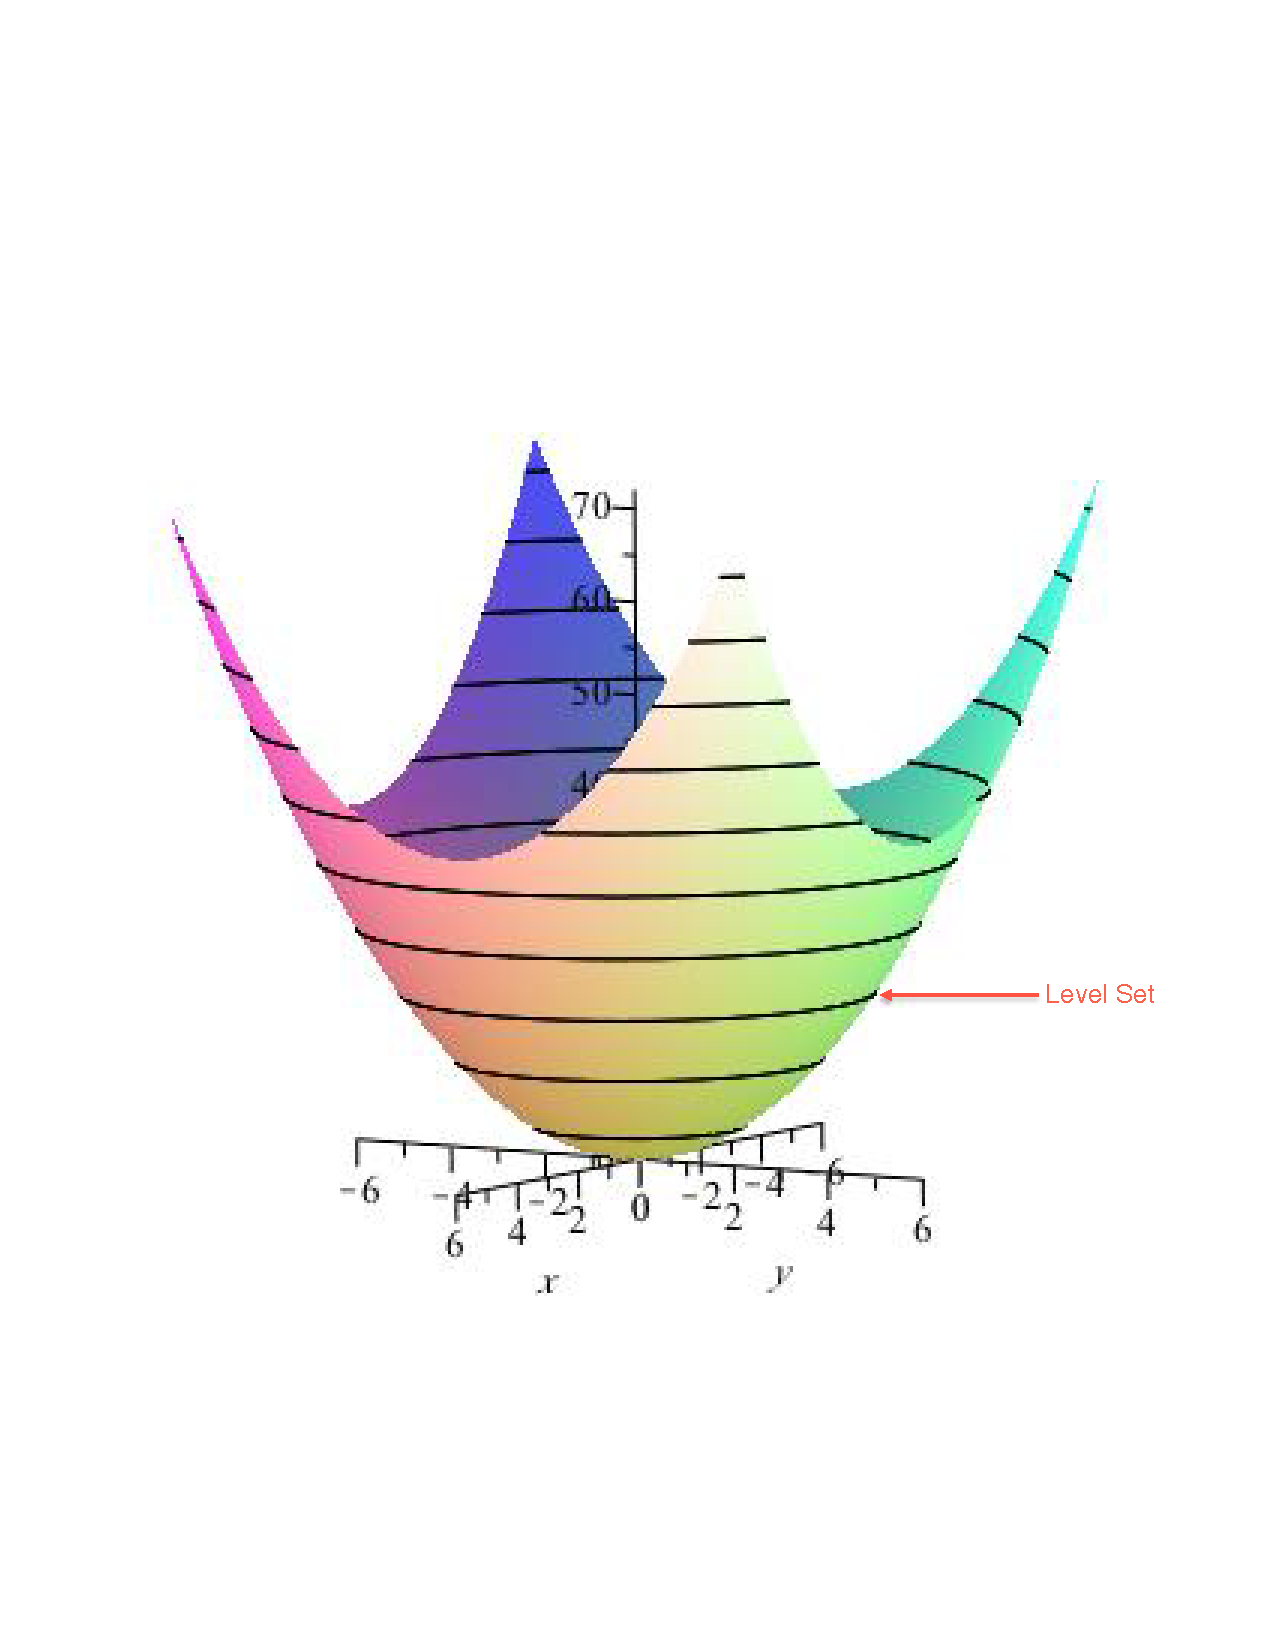
\includegraphics[scale=0.25]{LevelSetPlotNote.pdf}
\caption{Plot with Level Sets Projected on the Graph of $z$. The level sets existing in $\mathbb{R}^2$ while the graph of $z$ existing $\mathbb{R}^3$. The level sets have been projected onto their appropriate heights on the graph.}
\label{fig:LevelSet3D}
\end{figure}
\begin{figure}[ht]
\centering
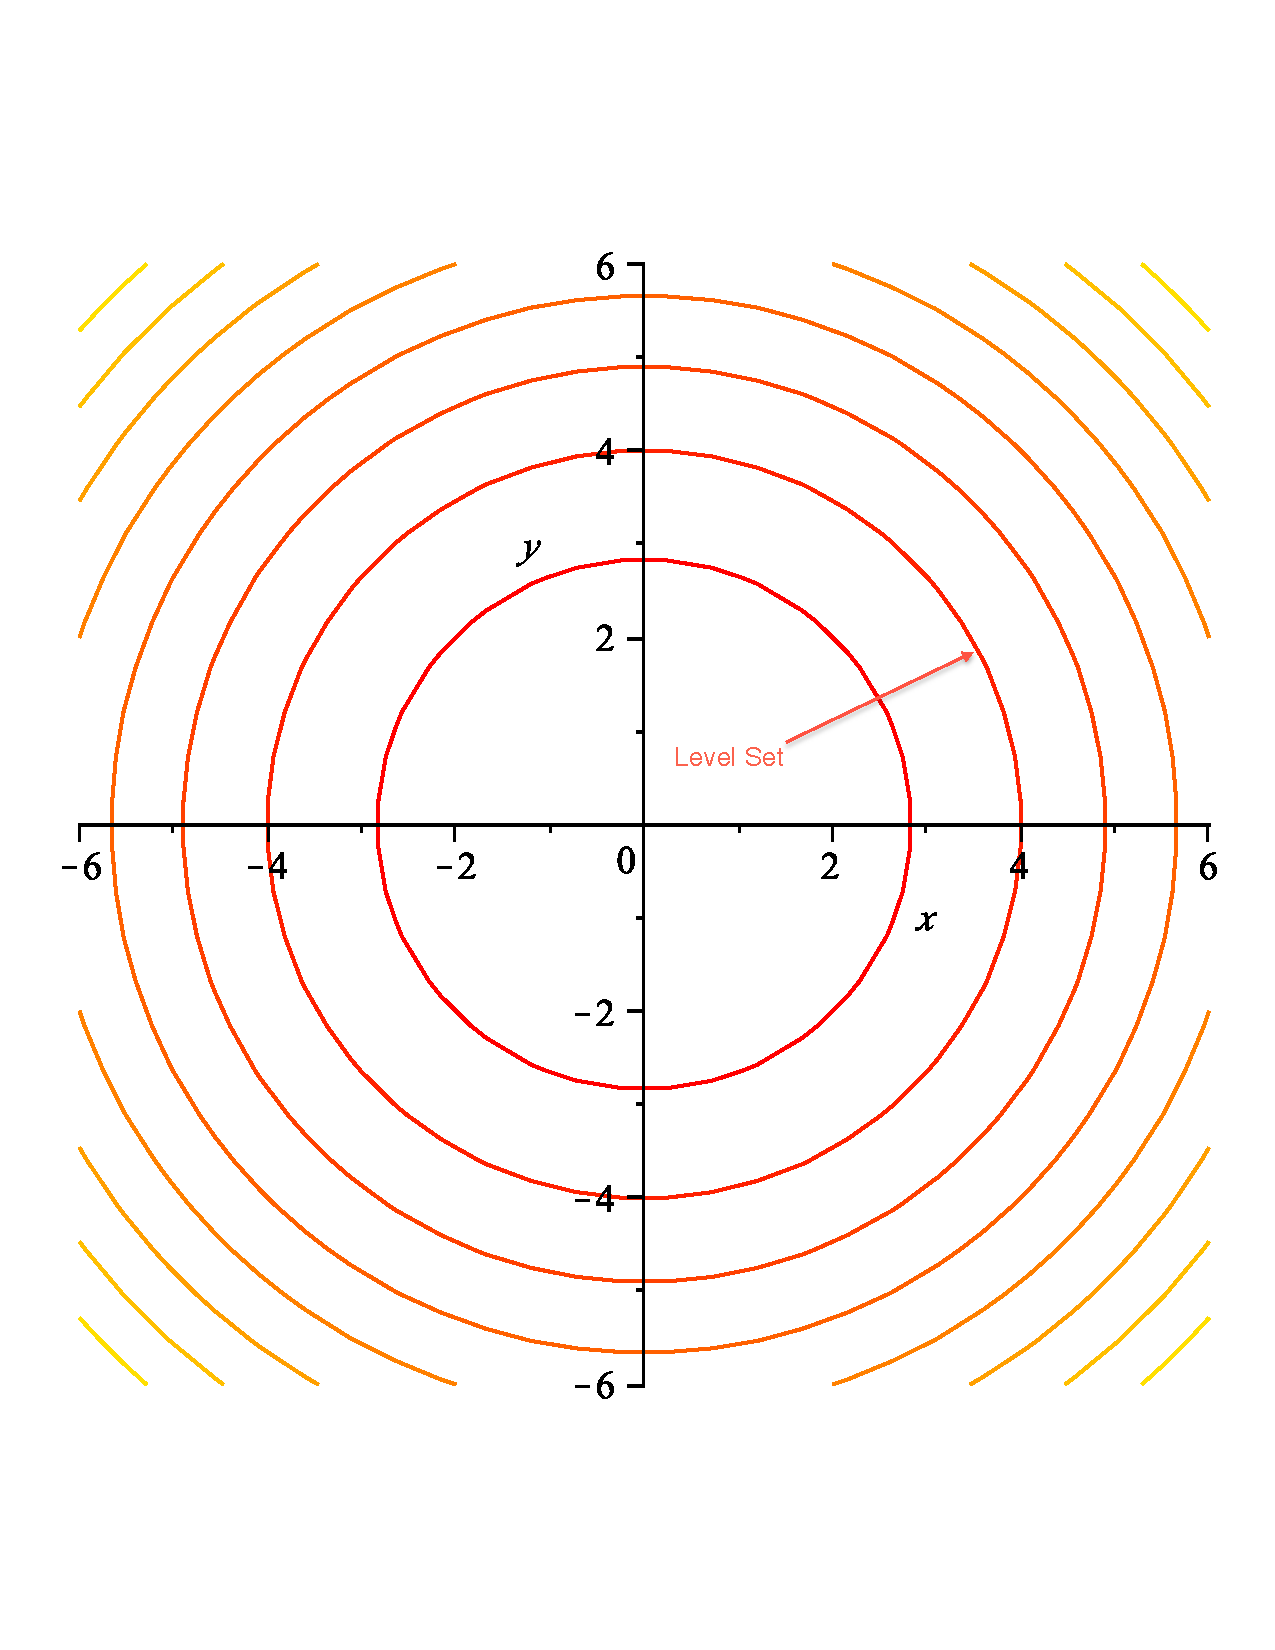
\includegraphics[scale=0.25]{ContourPlotNote.pdf}
\caption{Contour Plot of $z=x^2 + y^2$. The circles in $\mathbb{R}^2$ are the level sets of the function. The lighter the circle hue, the higher the value of $c$ that defines the level set.}
\label{fig:LevelSet2D}
\end{figure}
\label{ex:LevelSet}
\end{example}

\begin{definition}(Line) Let $\mathbf{x}_0,\mathbf{v} \in \mathbb{R}^n$. Then the \textit{line} defined by vectors $\mathbf{x}_0$ and $\mathbf{v}$ is the function $\mathbf{l}(t) = \mathbf{x}_0 + t\mathbf{v}$. Clearly $l : \mathbb{R} \rightarrow \mathbb{R}^n$. The vector $\mathbf{v}$ is called the direction of the line. 
\label{def:Line}
\end{definition} 

\begin{example}
Let $\mathbf{x_0} = (2,1)$ and let $\mathbf{v} = (2,2)$. Then the line defined by $\mathbf{x}_0$ and $\mathbf{v}$ is shown in Figure \ref{fig:LineExample}. The set of points on this line is the set $L = \{(x,y) \in \mathbb{R}^2 : x = 2 + 2t, y = 1 + 2t, t \in \mathbb{R}\}$. 
\begin{figure}[ht]
\centering
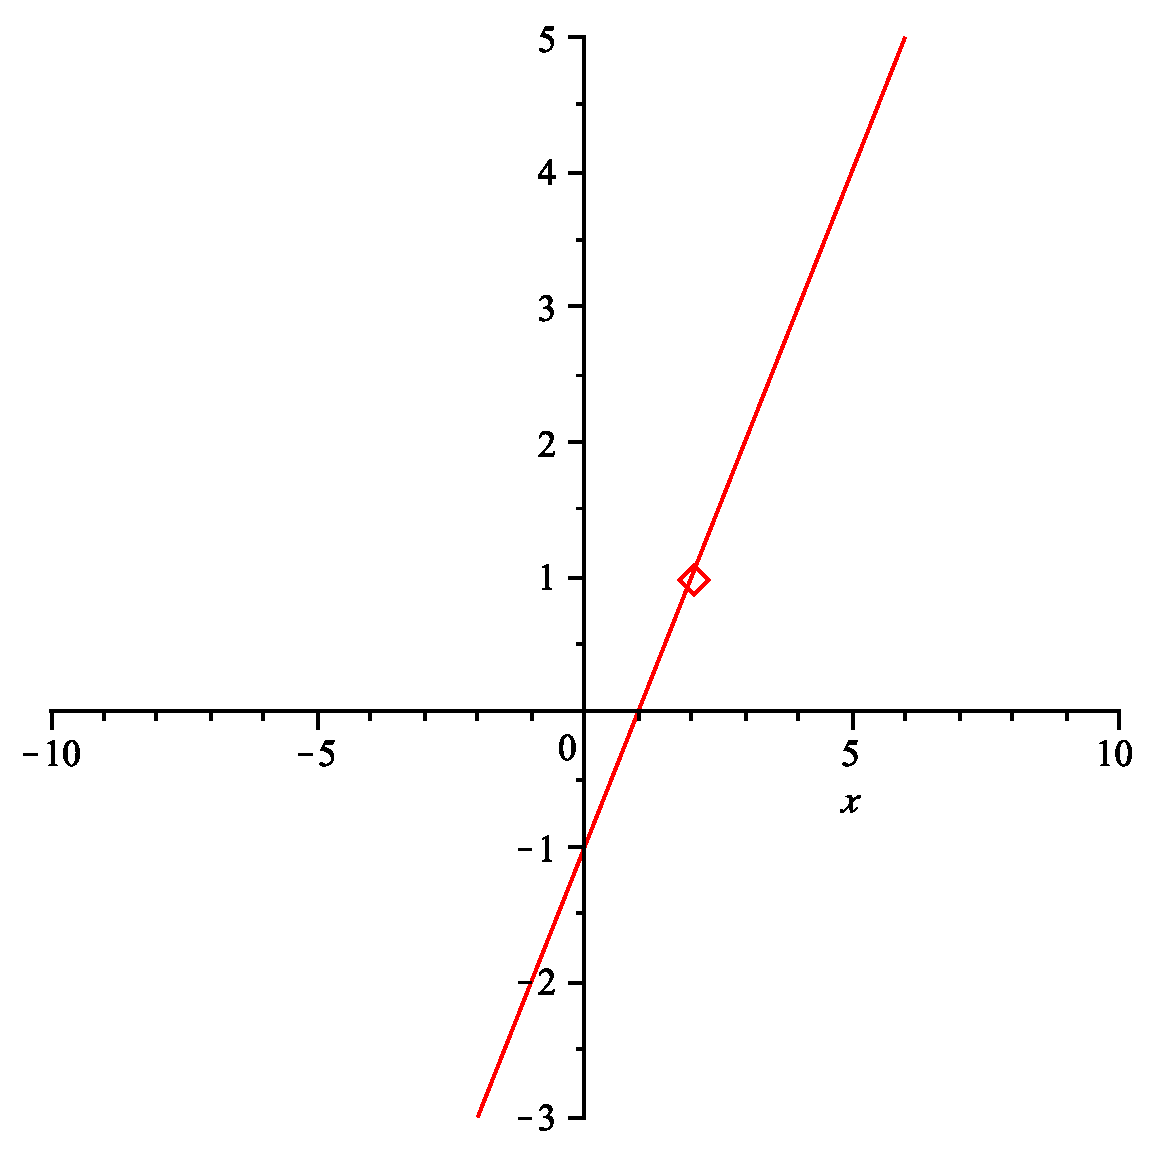
\includegraphics[scale=0.25]{LinePlot.pdf}
\caption{A Line Function: The points in the graph shown in this figure are in the set produced using the expression $\mathbf{x}_0 + \mathbf{v}t$ where $\mathbf{x_0} = (2,1)$ and let $\mathbf{v} = (2,2)$.}
\label{fig:LineExample}
\end{figure}
\label{ex:BasicLine}
\end{example}

\begin{definition}[Directional Derivative] Let $z:\mathbb{R}^n \rightarrow \mathbb{R}$ and let $\mathbf{v} \in \mathbb{R}^n$ be a vector (direction) in n-dimensional space. Then the directional derivative of $z$ at point $\mathbf{x}_0 \in\mathbb{R}^n$ in the direction of $\mathbf{v}$ is
\begin{equation}
\left.\frac{d}{dt}z(\mathbf{x}_0 + t\mathbf{v})\right\vert_{t=0}
\end{equation}
when this derivative exists.
\label{def:DirectionalDerivative}
\end{definition}

\begin{proposition} The directional derivative of $z$ at $\mathbf{x}_0$ in the direction $\mathbf{v}$ is equal to:
\begin{equation}
\lim_{h \rightarrow 0}\frac{z(\mathbf{x}_0 + h\mathbf{v}) - z(\mathbf{x}_0)}{h}
\end{equation}
\label{prop:DirecDeriv}
\end{proposition}

\begin{exercise} Prove Proposition \ref{prop:DirecDeriv}. [Hint: Use the definition of derivative for a univariate function and apply it to the definition of directional derivative and evaluate $t=0$.]
\end{exercise}
%\begin{proof} The definition of the derivative yields the expression:
%\begin{equation}
%\frac{d}{dt}z(\mathbf{x}_0 + t\mathbf{v}) = 
%\lim_{h \rightarrow 0}\frac{z(\mathbf{x}_0 + (t+h)\mathbf{v}) - z(\mathbf{x}_0 + t\mathbf{v})}{h},
%\end{equation}
%assuming that the limit exists. Evaluating the left and right hand sides at $t = 0$ yields:
%\begin{equation}
%\left.\frac{d}{dt}z(\mathbf{x}_0 + t\mathbf{v})\right\vert_{t=0} = 
%\lim_{h \rightarrow 0}\frac{z(\mathbf{x}_0 + h\mathbf{v}) - z(\mathbf{x}_0)}{h}
%\end{equation}
%This completes the proof.
%\end{proof}

\begin{definition}[Gradient]
Let $z:\mathbb{R}^n \rightarrow \mathbb{R}$ be a function and let $\mathbf{x}_0 \in \mathbb{R}^n$. Then the \textit{gradient} of $z$ at $\mathbf{x}_0$ is the vector in $\mathbb{R}^n$ given by:
\begin{equation}
\nabla z(\mathbf{x}_0) = \left(\frac{\partial z}{\partial x_1}(\mathbf{x}_0),\dots, \frac{\partial z}{\partial x_n}(\mathbf{x}_0)\right)
\end{equation}
\label{def:Gradient}
\end{definition}

Gradients are extremely important concepts in optimization (and vector calculus in general). Gradients have many useful properties that can be exploited. The relationship between the directional derivative and the gradient is of critical importance.

\begin{theorem} If $z:\mathbb{R}^n \rightarrow \mathbb{R}$ is differentiable, then all directional derivatives exist. Furthermore, the directional derivative of $z$ at $\mathbf{x}_0$ in the direction of $\mathbf{v}$ is given by:
\begin{equation}
\nabla z(\mathbf{x}_0) \cdot \mathbf{v}
\end{equation}
where $\cdot$ denotes the \textit{dot} product of two vectors.
\end{theorem}
\begin{proof} Let $\mathbf{l}(t) = \mathbf{x}_0 + \mathbf{v}t$. Then $\mathbf{l}(t) = (l_1(t),\dots,l_n(t))$; that is, $\mathbf{l}(t)$ is a vector function whose $i^{\text{th}}$ component is given by $l_i(t) = \mathbf{x}_{0_i} + \mathbf{v}_it$. 

Apply the chain rule:
\begin{equation}
\frac{dz(\mathbf{l}(t))}{dt} = 
	\frac{\partial z}{\partial l_1}\frac{dl_1}{dt} + \dots + 
	\frac{\partial z}{\partial l_n}\frac{dl_n}{dt}
\end{equation}
Thus:
\begin{equation}
\frac{d}{dt}z(\mathbf{l}(t)) = \nabla z\cdot\frac{d\mathbf{l}}{dt}
\end{equation}
Clearly $d\mathbf{l}/dt = \mathbf{v}$. We have $\mathbf{l}(0) = \mathbf{x}_0$. Thus:
\begin{equation}
\left.\frac{d}{dt}z(\mathbf{x}_0 + t\mathbf{v})\right\vert_{t=0} = 
	\nabla z(\mathbf{x}_0) \cdot \mathbf{v}
\end{equation}
\end{proof}

We now come to the two most important results about gradients, (i) the fact that they always point in the direction of steepest ascent with respect to the level curves of a function and (ii) that they are perpendicular (normal) to the level curves of a function. We can exploit this fact as we seek to maximize (or minimize) functions.

\begin{theorem} Let $z:\mathbb{R}^n \rightarrow \mathbb{R}$ be differentiable, $\mathbf{x}_0 \in \mathbb{R}^n$. If $\nabla z(\mathbf{x}_0) \neq 0$, then $\nabla z(\mathbf{x}_0)$ points in the direction in which $z$ is increasing fastest.
\end{theorem}
\begin{proof} Recall $\nabla z(\mathbf{x}_0)\cdot \mathbf{v}$ is the directional derivative of $z$ in direction $\mathbf{v}$ at $\mathbf{x}_0$. Assume that $\mathbf{v}$ is a unit vector. We know that:
\begin{equation}
\nabla z(\mathbf{x}_0)\cdot \mathbf{v}  = ||\nabla z(\mathbf{x}_0)||\cos\theta
\end{equation}
(because we assumed $\mathbf{v}$ was a unit vector) where $\theta$ is the angle between the vectors $\nabla z(\mathbf{x}_0)$ and $\mathbf{v}$. The function $\cos\theta$ is largest when $\theta = 0$, that is when $\mathbf{v}$ and $\nabla z(\mathbf{x}_0)$ are parallel vectors. (If $\nabla z(\mathbf{x}_0) = 0$, then the directional derivative is zero in all directions.)
\end{proof}

\begin{theorem} Let $z:\mathbb{R}^n \rightarrow \mathbb{R}$ be differentiable and let $\mathbf{x}_0$ lie in the level set $S$ defined by $z(\mathbf{x}) = k$ for fixed $k \in \mathbb{R}$. Then $\nabla z(\mathbf{x}_0)$ is normal to the set $S$ in the sense that if $\mathbf{v}$ is a tangent vector at $t = 0$ of a path $\mathbf{c}(t)$ contained entirely in $S$ with $\mathbf{c}(0) = \mathbf{x}_0$, then $\nabla z(\mathbf{x}_0) \cdot \mathbf{v} = 0$. 
\label{thm:GradPerpLevelSet}
\end{theorem}

\begin{remark} Before giving the proof, we illustrate this theorem in Figure \ref{fig:LevelSetWithVector}. The function is $z(x,y) = x^4+y^2+2xy$ and $\mathbf{x}_0 = (1,1)$. At this point $\nabla z(\mathbf{x}_0) = (6,4)$. We include the tangent line to the level set at the point (1,1) to illustrate the normality of the gradient to the level curve at the point.
\end{remark}

\begin{figure}[htbp]
\centering
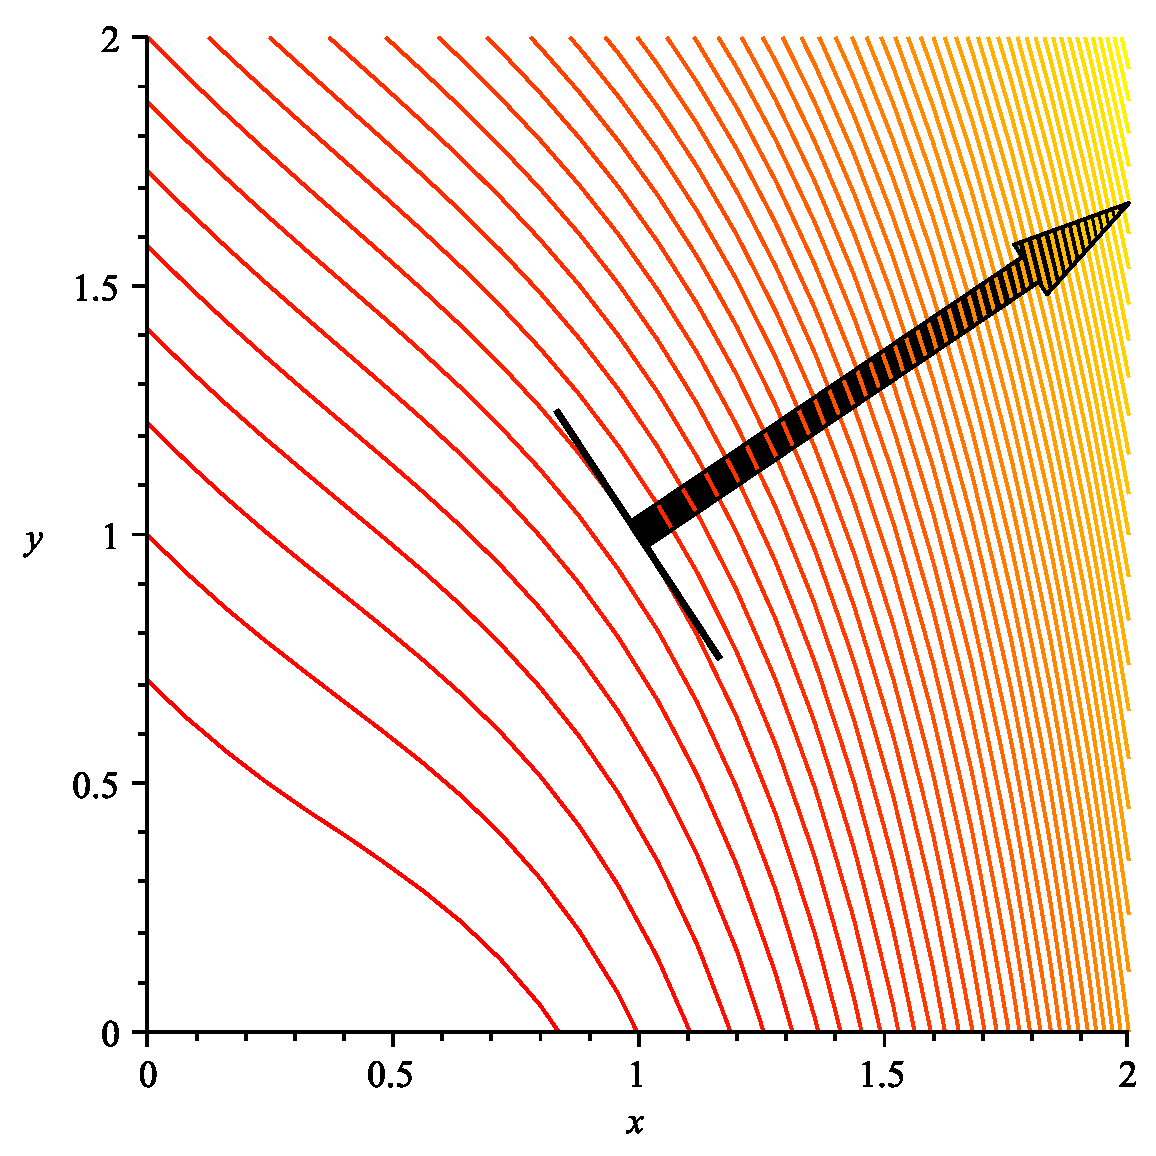
\includegraphics[scale=0.35]{LevelSetsWithVector.pdf}
\caption{A Level Curve Plot with Gradient Vector: We've scaled the gradient vector in this case to make the picture understandable. Note that the gradient is perpendicular to the level set curve at the point $(1,1)$, where the gradient was evaluated. You can also note that the gradient is pointing in the direction of steepest ascent of $z(x,y)$.}
\label{fig:LevelSetWithVector}
\end{figure}

\begin{proof} As stated, let $\mathbf{c}(t)$ be a curve in $S$. Then $\mathbf{c}:\mathbb{R} \rightarrow \mathbb{R}^n$ and $z(\mathbf{c}(t) ) = k$ for all $t \in \mathbb{R}$. Let $\mathbf{v}$ be the tangent vector to $\mathbf{c}$ at $t = 0$; that is:
\begin{equation}
\left.\frac{d\mathbf{c}(t)}{dt}\right|_{t=0} = \mathbf{v}
\end{equation}
Differentiating $z(\mathbf{c}(t))$ with respect to $t$ using the chain rule and evaluating at $t = 0$ yields:
\begin{equation}
\left.\frac{d}{dt}z(\mathbf{c}(t))\right|_{t=0} = \nabla z(\mathbf{c}(0))\cdot\mathbf{v} = \nabla z(\mathbf{x}_0) \cdot \mathbf{v} = 0
\end{equation}
Thus $\nabla z(\mathbf{x}_0)$ is perpendicular to $\mathbf{v}$ and thus normal to the set $S$ as required.
\end{proof}

\begin{remark}There's a simpler proof of this theorem in the case of a mapping $z : \mathbb{R}^2 \rightarrow \mathbb{R}$. For any such function $z(x,y)$, we know that a level set is an implicitly defined curve given by the expression
\begin{displaymath}
z(x,y) = k
\end{displaymath}
where $k \in \mathbb{R}$. We can compute the slope of any tangent line to this curve at some point $(x_0,y_0)$ with implicit differentiation. We have:
\begin{displaymath}
\left(\frac{d}{dx}\right) z(x,y) = k \left(\frac{d}{dx}\right)
\end{displaymath}
yields:
\begin{displaymath}
\frac{\partial z}{\partial x} + \frac{\partial z}{\partial y}\frac{dy}{dx}  = 0 
\end{displaymath}
Then the slope of the tangent line is given by:
\begin{displaymath}
\frac{dy}{dx} = \frac{-\partial z/\partial x}{\partial z/\partial y}
\end{displaymath}
By $z_x(x_0,y_0)$ we mean $\partial z/\partial x$ evaluated at $(x_0,y_0)$ and by $z_y(x_0,y_0)$ we mean $\partial z/\partial y$ evaluated at $(x_0,y_0)$. Then the slope of the tangent line to the curve $z(x,y) = k$ at $(x_0,y_0)$ is:
\begin{displaymath}
m = \frac{-z_x(x_0,y_0)}{z_y(x_0,y_0)}
\end{displaymath}
An equation for the tangent line at this point is:
\begin{equation}
y - y_0 = m(x - x_0)
\label{eqn:PointSlope}
\end{equation}
We can compute a vector that is parallel to this line by taking two points on the line, $(x_0,y_0)$ and $(x_1, y_1)$ and computing the vector $(x_1 - x_0, y_1 - y_0)$. We know that:
\begin{displaymath}
y_1 - y_0 = m(x_1 - x_0)
\end{displaymath}
because any pair $(x_1,y_1)$ on the tangent line must satisfy Equation \ref{eqn:PointSlope}. Thus we have the vector $\mathbf{v} = (x_1 - x_0, m(x_1 - x_0))$ parallel to the tangent line. Now we compute the dot product of this vector with the gradient of the function:
\begin{displaymath}
\nabla z(x_0,y_0) = (z_x(x_0,y_0), z_y(x_0,y_0))
\end{displaymath}
We obtain:
\begin{multline*}
\nabla z(x_0,y_0)\cdot\mathbf{v} = z_x(x_0,y_0)\left(x_1 - x_0\right) + z_y(x_0,y_0)\left(m(x_1 - x_0)\right) = \\z_x(x_0,y_0)\left(x_1 - x_0\right) + 
z_y(x_0,y_0)\left(\frac{-z_x(x_0,y_0)}{z_y(x_0,y_0)}(x_1 - x_0)\right)
 = \\
z_x(x_0,y_0)\left(x_1 - x_0\right) + \left(-z_x(x_0,y_0)(x_1 - x_0)\right) = 0
\end{multline*}
Thus, $\nabla z(x_0,y_0)$ is perpendicular to $\mathbf{v}$ as we expected from Theorem \ref{thm:GradPerpLevelSet}
\end{remark}

\begin{example} Let's demonstrate the previous remark and Theorem \ref{thm:GradPerpLevelSet}. Consider the function $z(x,y) = x^4 + y^2 + 2xy$ with a point $(x_0,y_0)$. Any level curve of the function is given by: $x^4 + y^2 + 2xy = k$. Taking the implicit derivative we obtain:
\begin{displaymath}
\left(\frac{d}{dx}\right)x^4 + y^2 + 2xy = k\left(\frac{d}{dx}\right) \implies 
4x^3 + 2y\frac{dy}{dx} + 2y + 2x\frac{dy}{dx} = 0
\end{displaymath}
Note that to properly differentiate $2xy$ implicitly, we needed to use the product rule from calculus. Now, we can solve for the slope of the tangent line to the curve at point $(x_0,y_0)$ as:
\begin{displaymath}
m = \left(\frac{dy}{dx}\right) = \frac{-4x_0^3 - 2y_0}{2y_0 + 2x_0}
\end{displaymath}
Our tangent line is then described the equation:
\begin{displaymath}
y - y_0 = m(x - x_0)
\end{displaymath}
Using the same reasoning we did in the remark, a vector parallel to this line is given by $(x_1 - x_0, y_1 - y_0)$ where $(x_1, y_1)$ is another point on the tangent line. Then we know that:
\begin{displaymath}
y_1 - y_0 = m(x_1 - x_0)
\end{displaymath}
and thus our vector is $\mathbf{v} = (x_1 - x_0, m(x_1 - x_0))$. Now, computing the gradient of $z(x,y)$ at $(x_0,y_0)$ is:
\begin{displaymath}
\nabla z(x_0,y_0) = (4x_0^3 + 2y_0, 2y_0 + 2x_0)
\end{displaymath} 
Lastly we compute:
\begin{multline*}
\nabla z(x_0,y_0)\cdot\mathbf{v} = \left(4x_0^3 + 2y_0\right)(x_1 - x_0) + 
\left(2y_0 + 2x_0\right)\left(m(x_1 - x_0)\right) = \\
\left(4x_0^3 + 2y_0\right)(x_1 - x_0) + \left(2y_0 + 2x_0\right)\left(\frac{-4x_0^3 - 2y_0}{2y_0 + 2x_0}(x_1 - x_0)\right) = \\
\left(4x_0^3 + 2y_0\right)(x_1 - x_0) + \left(-4x_0^3 - 2y_0\right)(x_1 - x_0) = 0
\end{multline*}
Thus, for any point $(x_0,y_0)$ on a level curve of $z(x,y) = x^4 + y^2 + 2xy$ we know that the gradient at that point is perpendicular to a tangent line (vector) to the curve at the point $(x_0,y_0)$. 

It is interesting to note that one can compute the slope of the tangent line (and its equation) in Figure \ref{fig:LevelSetWithVector}. Here $(x_0,y_0) = (1,1)$, thus the slope of the tangent line is:
\begin{displaymath}
m = \frac{-4x_0^3 - 2y_0}{2y_0 + 2x_0} = \frac{-6}{4} = \frac{-3}{2}
\end{displaymath}
The equation for the line displayed in Figure \ref{fig:LevelSetWithVector} is:
\begin{displaymath}
y - 1 = \frac{-3}{2}(x - 1)
\end{displaymath}
\end{example}

\begin{exercise} In this exercise you will use elementary calculus (and a little bit of vector algebra) to show that the gradient of a simple function is perpendicular to its level sets:
\begin{description*}
\item[(a)] Plot the level sets of $z(x,y) = x^2 + y^2$. Draw the gradient at the point $(x,y) = (2,0)$. Convince yourself that it is normal to the level set $x^2 + y^2 = 4$. 

\item[(b)] Now, choose any level set $x^2 + y^2 = k$. Use implicit differentiation to find $dy/dx$. This is the slope of a tangent line to the circle $x^2 + y^2 = k$. Let $(x_0,y_0)$ be a point on this circle.

\item[(c)] Find an expression for a vector parallel to the tangent line at $(x_0,y_0)$ [Hint: you can use the slope you just found.] 

\item[(d)] Compute the gradient of $z$ at $(x_0,y_0)$ and use it and the vector expression you just computed to show that two vectors are perpendicular. [Hint: use the dot product.]
\end{description*}
\end{exercise} 

\section{Gradients, Constraints and Optimization}
Since we're talking about optimization (i.e., minimizing or maximizing a certain function subject to some constraints), it follows that we should be interested in the gradient, which indicates the direction of greatest increase in a function. This information will be used in maximizing a function. Logically, the negation of the gradient will point in the direction of greatest decrease and can be used in minimization. We'll formalize these notions in the study of linear programming. We make one more definition:

\begin{definition}[Binding Constraint] Let $g(\mathbf{x}) \leq b$ be a constraint in an optimization problem. If at point $\mathbf{x}_0 \in \mathbb{R}^n$ we have $g(\mathbf{x}_0) = b$, then the constraint is said to be \textit{binding}. Clearly equality constraints $h(\mathbf{x}) = r$ are always binding.
\end{definition}

\begin{example}[Continuation of Example \ref{ex:GoatExample}] Let's look at the level curves of the objective function and their relationship to the constraints at the point of optimality $(x,y) = (25,25)$. In Figure \ref{fig:Goat2DPlot} we see the level curves of the objective function (the hyperbolas) and the feasible region shown as shaded. The elements in the feasible regions are all values for $x$ and $y$ for which $2x + 2y \leq 100$ and $x,y \geq 0$. You'll note that at the point of optimality the level curve $xy = 625$ is tangent to the equation $2x + 2y = 100$; i.e., the level curve of the objective function is tangent to the binding constraint.
\begin{figure}[htbp]
\centering
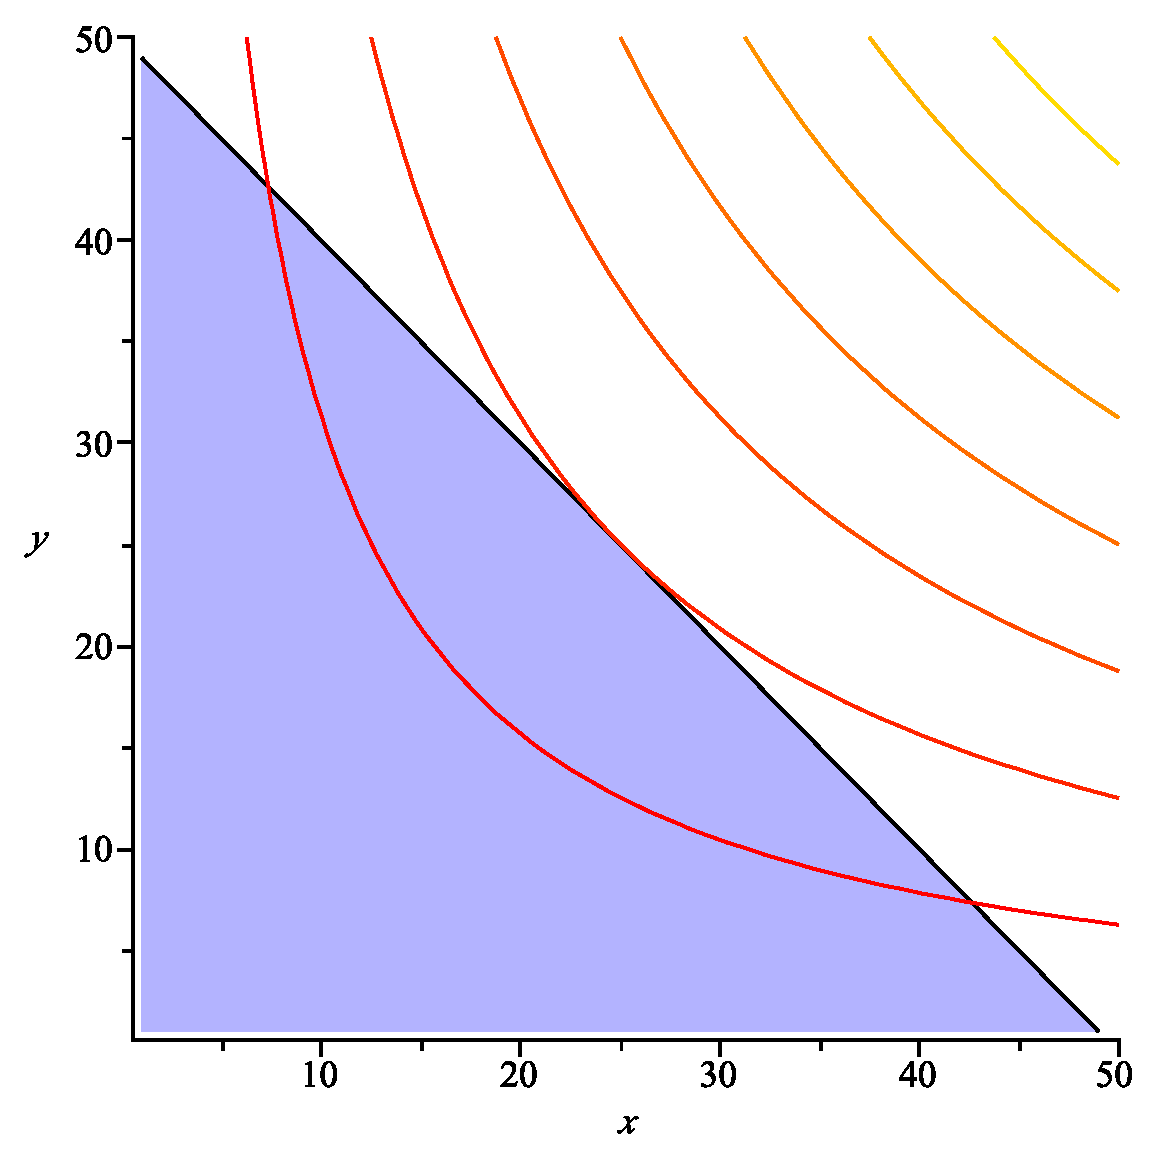
\includegraphics[scale=0.35]{GoatConstraintObjective.pdf}
\caption{Level Curves and Feasible Region: At optimality the level curve of the objective function is tangent to the binding constraints.}
\label{fig:Goat2DPlot}
\end{figure}

If you look at the gradient of $A(x,y)$ at this point it has value $(25,25)$. We see that it is pointing in the direction of increase for the function $A(x,y)$ (as should be expected) but more importantly let's look at the gradient of the function $2x + 2y$. It's gradient is $(2,2)$, which is just a scaled version of the gradient of the objective function. Thus the gradient of the objective function is just a dilation of gradient of the binding constraint. This is illustrated in Figure \ref{fig:Goat2DPlotWithGrad}.
\begin{figure}[htbp]
\centering
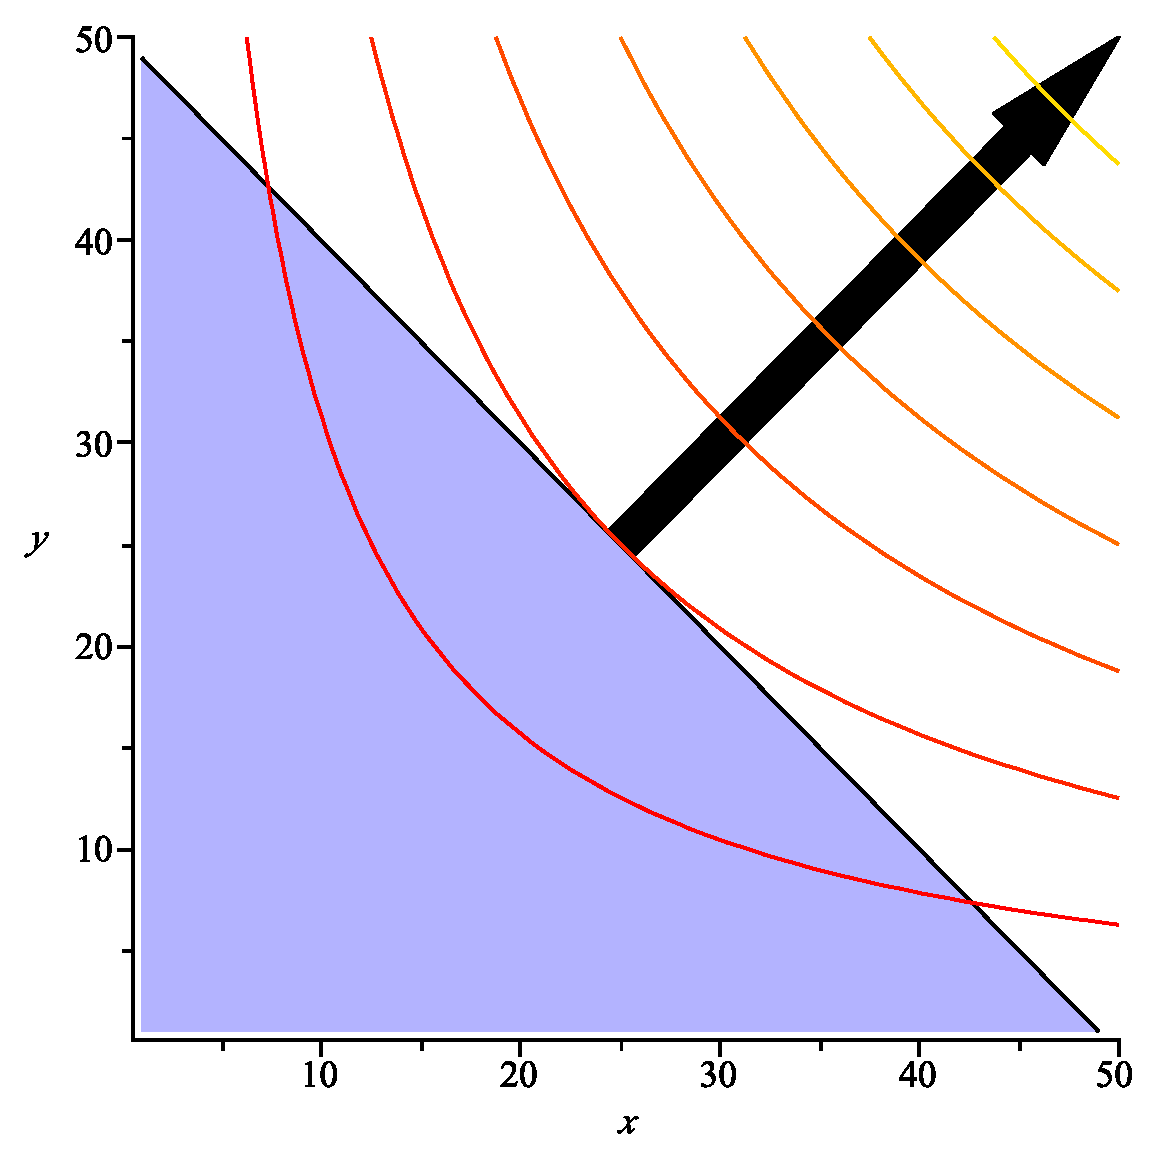
\includegraphics[scale=0.35]{GoatConstraintObjectiveWithGrad.pdf}
\caption{Gradients of the Binding Constraint and Objective: At optimality the gradient of the binding constraints and the objective function are \textit{scaled versions of each other}.}
\label{fig:Goat2DPlotWithGrad}
\end{figure}
\end{example}

The elements illustrated in the previous example are true in general. You may have discussed a simple example of these when you talked about \textit{Lagrange Multipliers} in Vector Calculus (Math 230/231). We'll revisit these concepts later when we talk about \textit{duality theory} for linear programs. We'll also discuss the gradients of the binding constraints with respect to optimality when we discuss linear programming. 

\begin{exercise} Plot the level sets of the objective function and the feasible region in Exercise \ref{exer:Can}. At the point of optimality you identified, show that the gradient of the objective function is a scaled version of the gradient (linear combination) of the binding constraints.
\end{exercise}

\chapter{Graphically Solving Linear Programs}
\todoChapter{ 50\% complete. Goal 80\% completion date: July 20\\
Notes: }
\begin{outcome}
\begin{enumerate}
\item[A.] Learn how to plot the feasible region and the objective function.
\item[B.] Identify and compute extreme points of the feasible region.
\item[C.] Find the optimal solution(s) to a linear program graphically.
\item[D.] Classify the type of result of the problem as infeasible, unbounded, unique optimal solution, or infinitely many optimal solutions.
\end{enumerate}
\end{outcome}

Linear Programs (LP's) with two variables can be solved graphically by plotting the feasible region along with the level curves of the objective function.\footnote{Special thanks to Joshua Emmanual and Christopher Griffin for sharing their content to help put this section together. Proper citations and referenes are forthcoming.} We will show that we can find a point in the feasible region that maximizes the objective function using the level curves of the objective function.

We will begin with an easy example that is bounded and investigate the structure of the feasible region.  We will then explore other examples.
\section{Nonempty and Bounded Problem}
\todoSection{ 20\% complete. Goal 80\% completion date: July 20\\
Notes: Need to work on this section.}
Consider the problem
\begin{align*}
\max \quad & 2 X+5 Y \\
\text { s.t. } \quad 
&X+2 Y \leq 16 \\
&5 X+3 Y \leq  45 \\
&X, Y  \geq 0
\end{align*}

We want to start by plotting the \emph{feasible region}, that is, the set points $(X,Y)$ that satisfy all the constraints. 

We can plot this by first plotting the four lines
\begin{itemize}
\item $X+2 Y = 16$
\item $5 X+3 Y = 45$
\item $X = 0$
\item $Y = 0$
\end{itemize}
and then shading in the side of the space cut out by the corresponding inequality.
\begin{center}
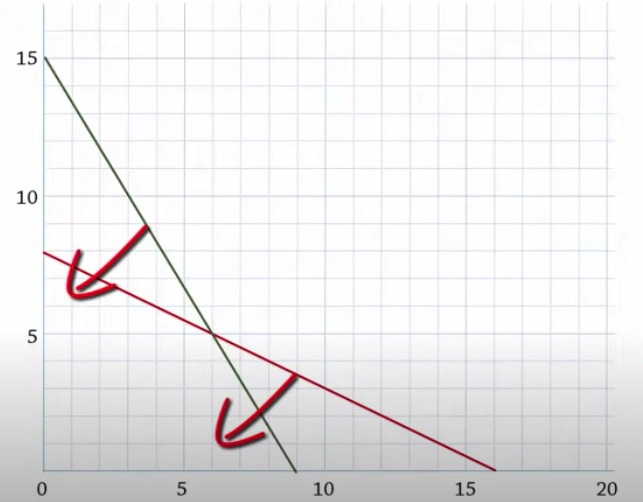
\includegraphics[scale = 0.4]{screenshots/example0-inequalities}
\end{center}

The resulting feasible region can then can be shaded in as the region that satisfies all the inequalties.

\begin{center}
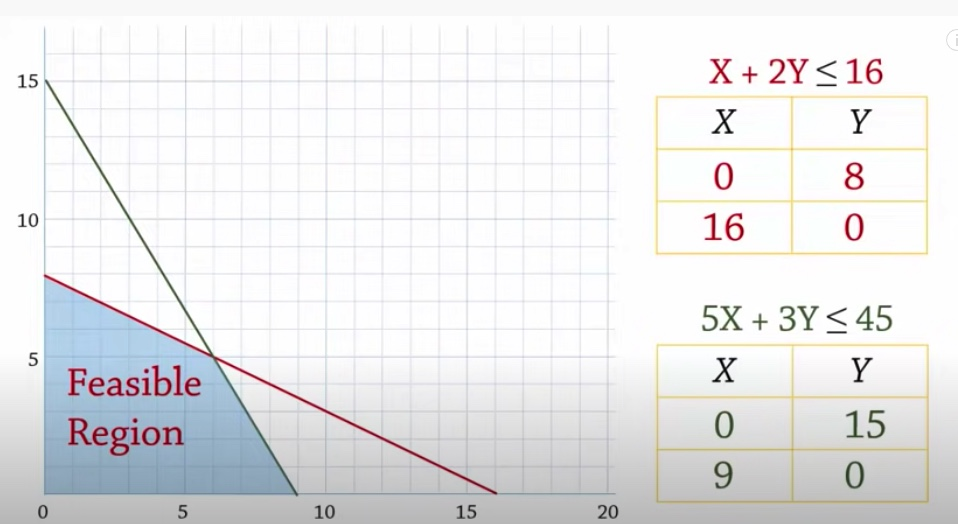
\includegraphics[scale = 0.4]{screenshots/example0-feasible-region}
\end{center}

Notice that the feasible region is nonempty (it has points that satisfy all the inequalities) and also that it is bounded (the feasible points dont continue infinitly in any direction).

We want to identify the \emph{extreme points} (i.e., the corners) of the feasible region. 
Understanding these points will be critical to understanding the optimal solutions of the model.
Notice that all extreme points can be computed by finding the intersection of 2 of the lines.   But!  Not all intersections of any two lines are feasible.  

We will later use the terminology \emph{basic feasible solution} for an extreme point of the feasible region, and \emph{basic solution} as a point that is the intersection of 2 lines, but is actually infeasible (does not satisfy all the constraints).

\begin{center}
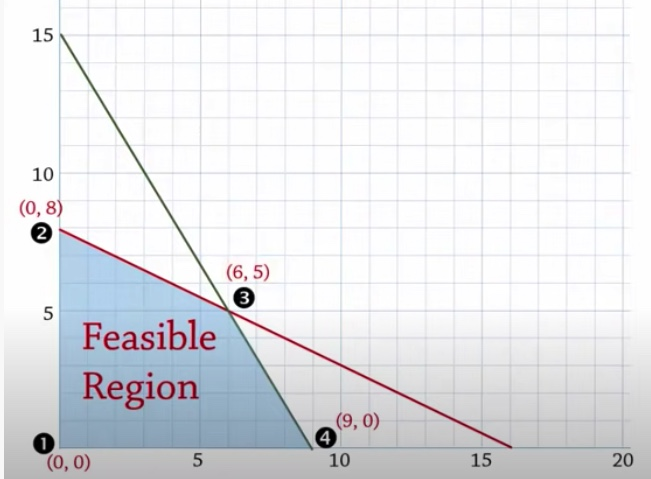
\includegraphics[scale = 0.4]{screenshots/example0-extreme-points}
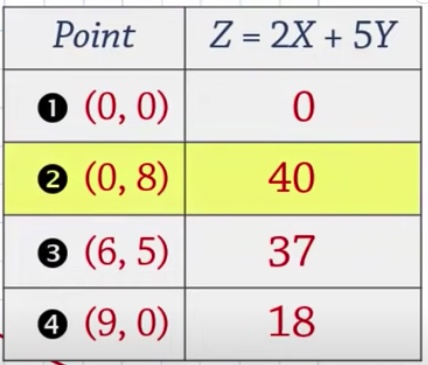
\includegraphics[scale = 0.4]{screenshots/example0-extreme-point-solutions}
\end{center}

\begin{theorem}{Optimal Extreme Point}{optimalextremepoint}
If the feasible region is nonempty and bounded, then there exists an optimal solution at an extreme point of the feasible region.
\end{theorem}

We will explore why this theorem is true, and also what happens when the feasible region does not satisfy the assumtions of either nonempty or bounded.
We illustrate the idea first using the problem from Example \ref{ex:ToyMaker}.

\begin{figure}[H] 
\centering
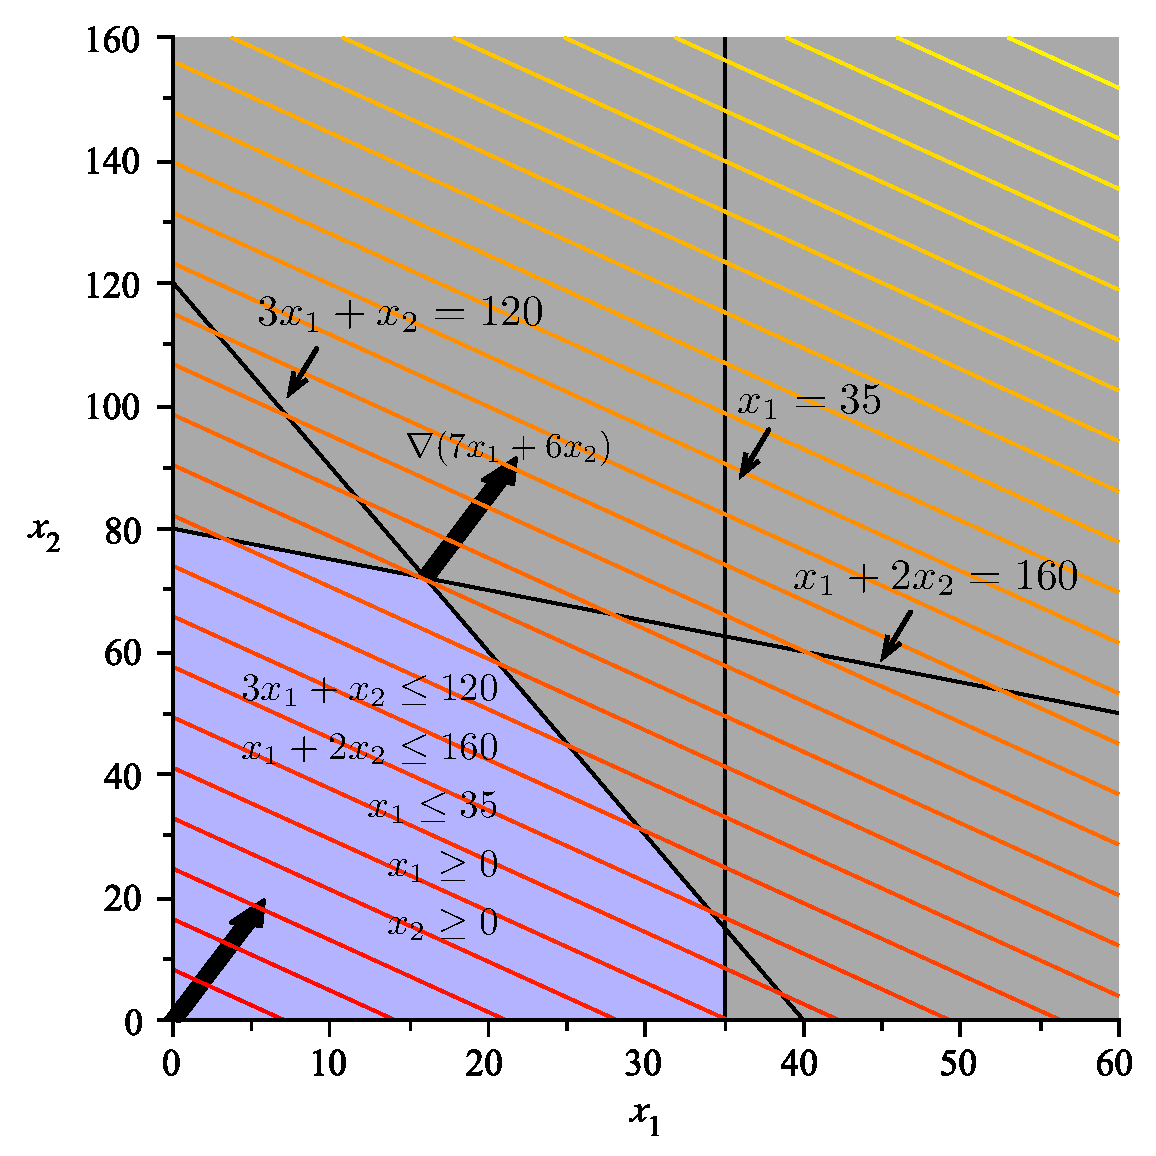
\includegraphics[scale=0.4]{FeasibleRegion.pdf}
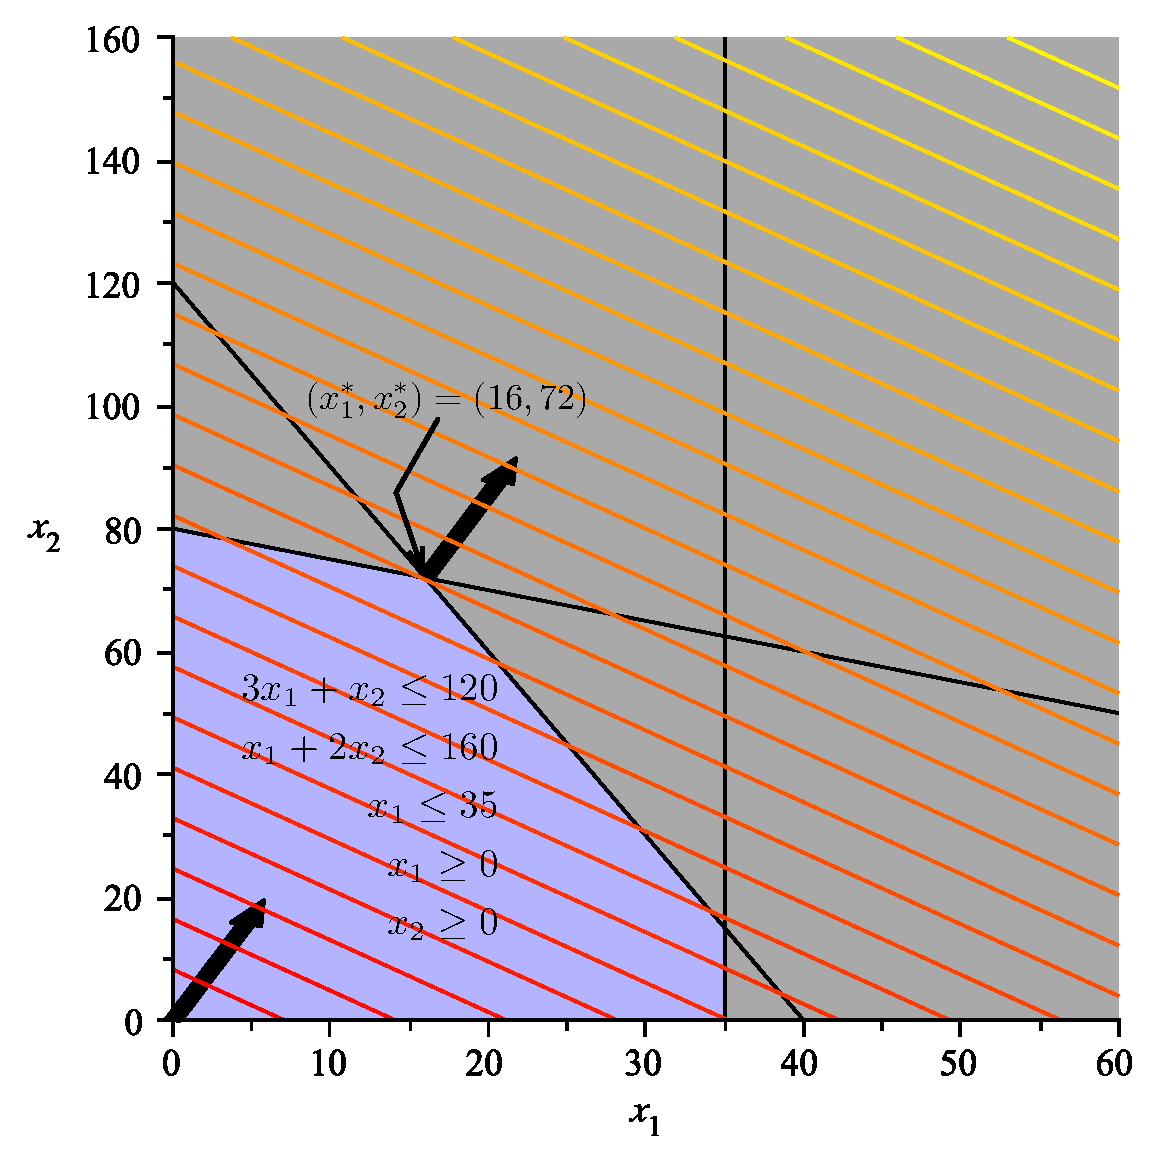
\includegraphics[scale=0.4]{FeasibleRegionWithMax.pdf}
\caption{Feasible Region and Level Curves of the Objective Function: The shaded region in the plot is the feasible region and represents the intersection of the five inequalities constraining the values of $x_1$ and $x_2$. On the right, we see the optimal solution is the ``last'' point in the feasible region that intersects a level set as we move in the direction of increasing profit.}
\label{fig:ToyExampleFeasibleRegion}
\end{figure}

\begin{example}{Continuation of Example \ref{ex:ToyMaker}}{}Let's continue the example of the Toy Maker begin in Example \ref{ex:ToyMaker}.  Solve this problem graphically.
\end{example}
\begin{solution} To solve the linear programming problem graphically, begin by drawing the feasible region. This is shown in the blue shaded region of Figure \ref{fig:ToyExampleFeasibleRegion}. 


After plotting the feasible region, the next step is to plot the level curves of the objective function. In our problem, the level sets will have the form:
\begin{displaymath}
7x_1 + 6x_2 = c \implies x_2 = \frac{-7}{6}x_1 + \frac{c}{6}
\end{displaymath}
This is a set of parallel lines with slope $-7/6$ and intercept $c/6$ where $c$ can be varied as needed. The level curves for various values of $c$ are parallel lines. In Figure \ref{fig:ToyExampleFeasibleRegion} they are shown in colors ranging from red to yellow depending upon the value of $c$. Larger values of $c$ are more yellow. 

To solve the linear programming problem, follow the level sets along the gradient (shown as the black arrow) until the last level set (line) intersects the feasible region. If you are doing this by hand, you can draw a single line of the form $7x_1 + 6x_2 = c$ and then simply draw parallel lines in the direction of the gradient $(7,6)$. At some point, these lines will fail to intersect the feasible region. The last line to intersect the feasible region will do so at a point that maximizes the profit. In this case, the point that maximizes $z(x_1,x_2) = 7x_1 + 6x_2$, subject to the constraints given, is $(x_1^*, x_2^*) = (16,72)$. 
\newpage
Note the point of optimality $(x_1^*, x_2^*) = (16,72)$ is at a corner of the feasible region. This corner is formed by the intersection of the two lines: $3x_1 + x_2 = 120$ and $x_1 + 2x_2 = 160$. In this case, the constraints 
\begin{gather*}
3x_1 + x_2 \leq 120\\
x_1 + 2x_2 \leq 160
\end{gather*}
are both \textit{binding}, while the other constraints are non-binding. In general, we will see that when an optimal solution to a linear programming problem exists, it will always be at the intersection of several binding constraints; that is, it will occur at a corner of a higher-dimensional polyhedron.  
\end{solution}

We can now define an algorithm for identifying the solution to a linear programing problem in two variables with a \textit{bounded} feasible region (see Algorithm \ref{alg:GraphLPBoundedUniqueSoln}): 
\begin{algorithm}
\caption{Algorithm for Solving a Two Variable Linear Programming Problem Graphically--Bounded Feasible Region, Unique Solution Case}
\label{alg:GraphLPBoundedUniqueSoln}
\begin{center}
\begin{minipage}[t]{\textwidth-1em}
\underline{\textbf{Algorithm for Solving a Linear Programming Problem Graphically}}\\
\textit{Bounded Feasible Region, Unique Solution}
\begin{enumerate*}
\item Plot the feasible region defined by the constraints.
\item Plot the level sets of the objective function.
\item For a maximization problem, identify the level set corresponding the greatest (least, for minimization) objective function value that intersects the feasible region. This point will be at a corner. 
\item The point on the corner intersecting the greatest (least) level set is a solution to the linear programming problem.  
\end{enumerate*}
\end{minipage}
\end{center}
\end{algorithm}

The example linear programming problem presented in the previous section has a single optimal solution. In general, the following outcomes can occur in solving a linear programming problem: 
\begin{enumerate*}
\item The linear programming problem has a unique solution. (We've already seen this.)
\item There are infinitely many alternative optimal solutions.
\item There is no solution and the problem's objective function can grow to positive infinity for maximization problems (or negative infinity for minimization problems). 
\item There is no solution to the problem at all. 
\end{enumerate*}

Case 3 above can only occur when the feasible region is unbounded; that is, it cannot be surrounded by a ball with finite radius. We will illustrate each of these possible outcomes in the next four sections. We will prove that this is true in a later chapter.



\section{Infinitely Many Optimal Solutions}
\todoSection{ 20\% complete. Goal 80\% completion date: July 20\\
Notes: Need to work on this section.}
It can happen that there is more than one solution.  In fact, in this case, there are infinitly many optimal solutions.  
We'll study a specific linear programming problem with an infinite number of solutions by modifying the objective function in Example \ref{ex:ToyMaker}. 
\begin{example}{Toy Maker Alternative Solutions}{ex:ToyMakerAltOptSoln}
Suppose the toy maker in Example \ref{ex:ToyMaker} finds that it can sell planes for a profit of $\$18$ each instead of $\$7$ each. The new linear programming problem becomes:
\begin{equation}
\left\{
\begin{aligned}
\max\;\;& z(x_1,x_2) = 18x_1 + 6x_2\\
s.t.\;\;&  3x_1 + x_2 \leq 120\\
& x_1 + 2x_2 \leq 160\\
& x_1 \leq 35\\
& x_1 \geq 0\\
& x_2 \geq 0
\end{aligned}
\right.
\label{eqn:ToyMakerAltOptSoln}
\end{equation}
\end{example}

\begin{solution}
Applying our graphical method for finding optimal solutions to linear programming problems yields the plot shown in Figure \ref{fig:ToyMakerAltOptSoln}. The level curves for the function $z(x_1,x_2) = 18x_1 + 6x_2$ are \textit{parallel} to one face of the polygon boundary of the feasible region. Hence, as we move further up and to the right in the direction of the gradient (corresponding to larger and larger values of $z(x_1, x_2)$) we see that there is not \textit{one} point on the boundary of the feasible region that intersects that level set with greatest value, but instead a side of the polygon boundary described by the line $3x_1 + x_2 = 120$ where $x_1 \in [16, 35]$. Let:
\begin{displaymath}
S = \{(x_1,x_2) | 3x_1 + x_2 \leq 120,\,x_1 + 2x_2 \leq 160,\,x_1 \leq 35,\,x_1,x_2 \geq 0\}
\end{displaymath} 
that is, $S$ is the feasible region of the problem. Then for any value of $x_1^* \in [16,35]$ and any value $x_2^*$ so that  $3x_1^* + x_2^* = 120$, we will have $z(x_1^*, x_2^*) \geq z(x_1, x_2)$ for all $(x_1,x_2) \in S$. Since there are infinitely many values that $x_1$ and $x_2$  may take on, we see this problem has an infinite number of alternative optimal solutions.
\begin{figure}[H]
\centering
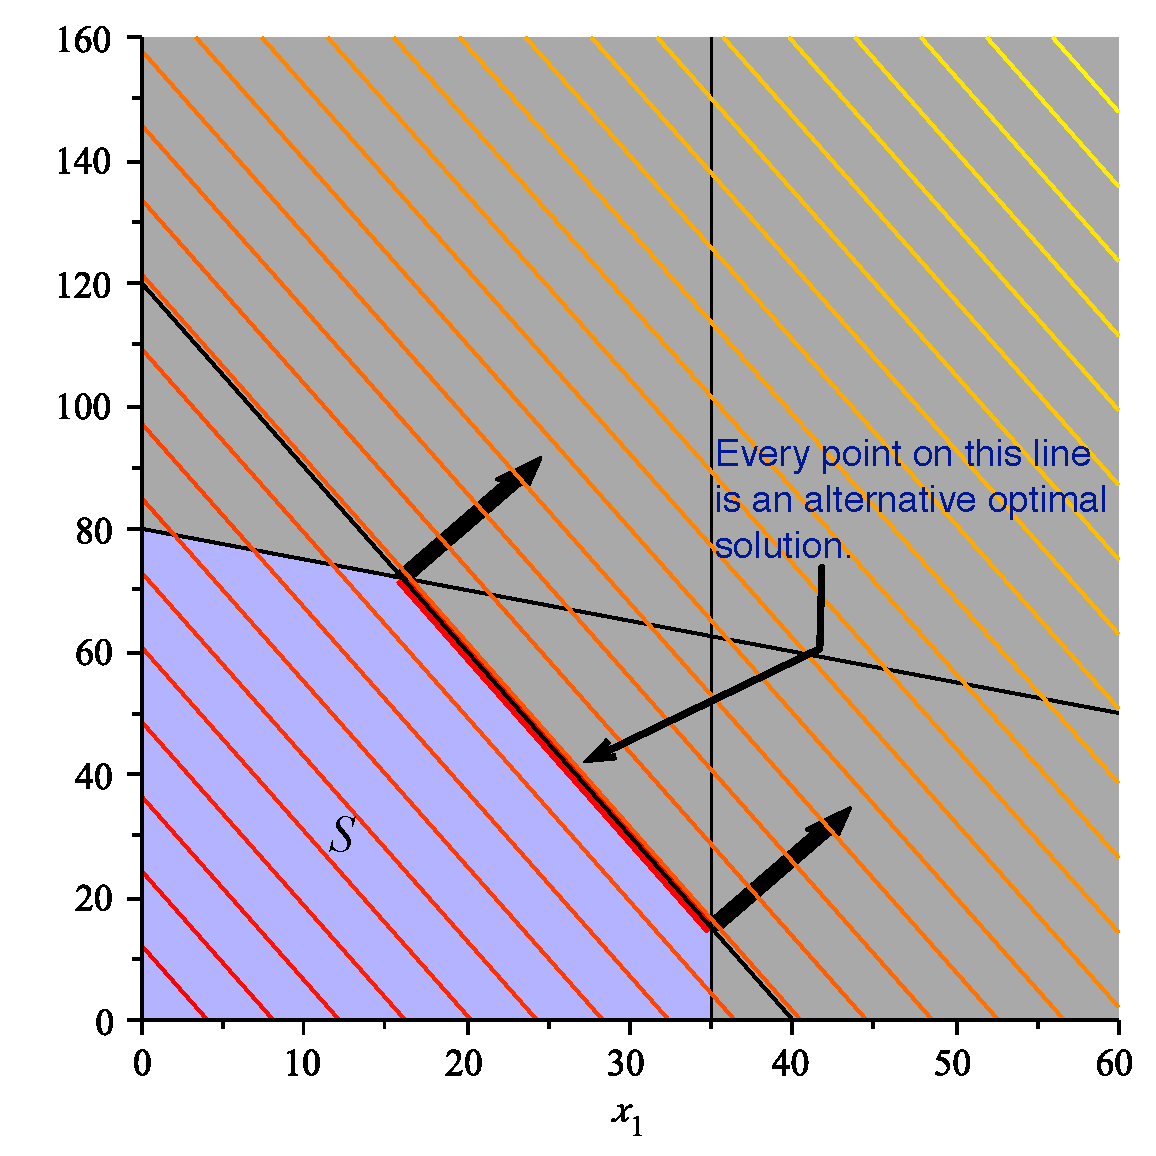
\includegraphics[scale=0.4]{AltOptSolns.pdf}
\caption{An example of infinitely many alternative optimal solutions in a linear programming problem. The level curves for $z(x_1,x_2) = 18x_1 + 6x_2$ are \textit{parallel} to one face of the polygon boundary of the feasible region. Moreover, this side contains the points of greatest value for $z(x_1,x_2)$ inside the feasible region. Any combination of $(x_1,x_2)$ on the line $3x_1 + x_2 = 120$ for $x_1 \in [16, 35]$ will provide the largest possible value $z(x_1,x_2)$ can take in the feasible region $S$.}
\label{fig:ToyMakerAltOptSoln}
\end{figure}
%\label{ex:ToyMakerAltOptSoln}
\end{solution}






\begin{exercise}{}{} Use the graphical method for solving linear programming problems to solve the linear programming problem you defined in Exercise \ref{exer:ChemicalPlant}.
\end{exercise}



Based on the example in this section, we can modify our algorithm for finding the solution to a linear programming problem graphically to deal with situations with an infinite set of alternative optimal solutions (see Algorithm \ref{alg:GraphLPBounded}):
\begin{algorithm}[H]
\caption{Algorithm for Solving a Two Variable Linear Programming Problem Graphically--Bounded Feasible Region Case}
\label{alg:GraphLPBounded}
\begin{center}
\begin{minipage}[t]{\textwidth-1em}
\underline{\textbf{Algorithm for Solving a Linear Programming Problem Graphically}}\\
\textit{Bounded Feasible Region}
\begin{enumerate*}
\item Plot the feasible region defined by the constraints.
\item Plot the level sets of the objective function.
\item For a maximization problem, identify the level set corresponding the greatest (least, for minimization) objective function value that intersects the feasible region. This point will be at a corner. 
\item The point on the corner intersecting the greatest (least) level set is a solution to the linear programming problem. 
\item \textbf{If the level set corresponding to the greatest (least) objective function value is parallel to a side of the polygon boundary next to the corner identified, then there are infinitely many alternative optimal solutions and any point on this side may be chosen as an optimal solution.} 
\end{enumerate*}
\end{minipage}
\end{center}
\end{algorithm}

\begin{exercise}{}{} Modify the linear programming problem from Exercise \ref{exer:ChemicalPlant} to obtain a linear programming problem with an infinite number of alternative optimal solutions. Solve the new problem and obtain a description for the set of alternative optimal solutions. [Hint: Just as in the example, $x_1$ will be bound between two value corresponding to a side of the polygon. Find those values and the constraint that is binding. This will provide you with a description of the form for any $x_1^* \in [a,b]$ and $x_2^*$ is chosen so that $cx_1^* + dx_2^* = v$, the point $(x_1^*, x_2^*)$ is an alternative optimal solution to the problem. Now you fill in values for $a$, $b$, $c$, $d$ and $v$.]
\end{exercise}

\section{Problems with No Solution} 
\todoSection{ 20\% complete. Goal 80\% completion date: July 20\\
Notes: Need to work on this section.}
Recall for \textit{any} mathematical programming problem, the feasible set or region is simply a subset of $\mathbb{R}^n$. If this region is empty, then there is no solution to the mathematical programming problem and the problem is said to be \textit{over constrained}. In this case, we say that the problem is \emph{infeasible}.  We illustrate this case for linear programming problems with the following example.
\begin{example}{Infeasible Problem}
 Consider the following linear programming problem:
\begin{equation}
\left\{
\begin{aligned}
\max\;\;& z(x_1,x_2) = 3x_1 + 2x_2\\
s.t.\;\;&  \frac{1}{40}x_1 + \frac{1}{60}x_2 \leq 1\\
& \frac{1}{50}x_1 + \frac{1}{50}x_2 \leq 1\\
& x_1 \geq 30\\
& x_2 \geq 20
\end{aligned}
\right.
\label{eqn:LPInfeasible}
\end{equation}
\end{example}
\begin{solution}
The level sets of the objective and the constraints are shown in Figure \ref{fig:LPInfeasible}. 
\begin{figure}[H]
\centering
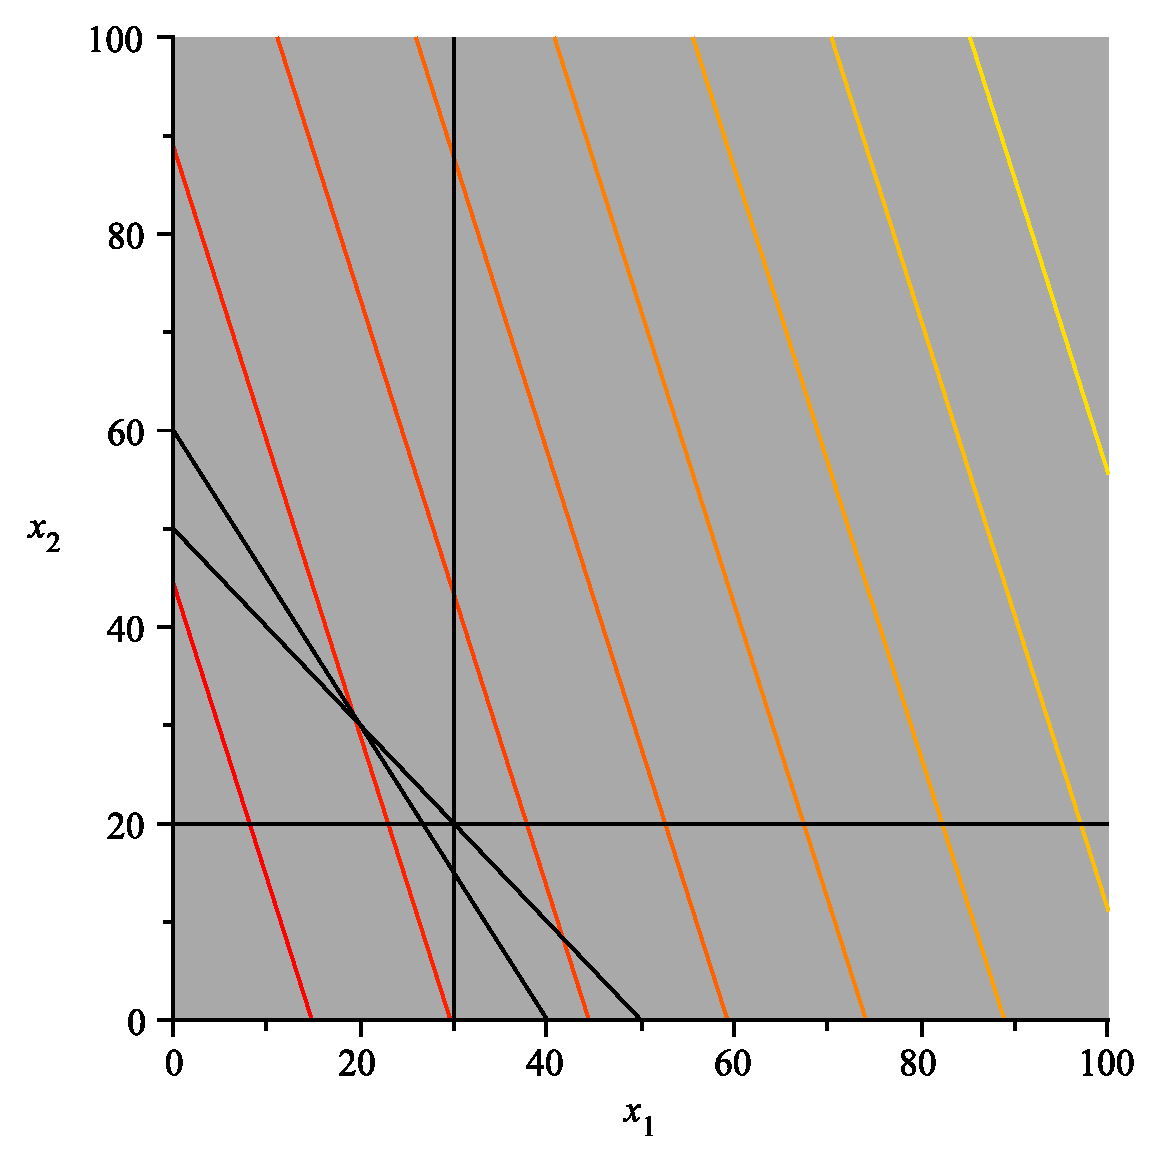
\includegraphics[scale=0.4]{LPNoSoln.pdf}
\caption{A Linear Programming Problem with no solution. The feasible region of the linear programming problem is empty; that is, there are no values for $x_1$ and $x_2$ that can simultaneously satisfy all the constraints. Thus, no solution exists.}
\label{fig:LPInfeasible}
\end{figure}

The fact that the feasible region is empty is shown by the fact that in Figure \ref{fig:LPInfeasible} there is no blue region--i.e., all the regions are gray indicating that the constraints are not satisfiable.
\label{ex:LPNoSoln}
\end{solution} 
Based on this example, we can modify our previous algorithm for finding the solution to linear programming problems graphically (see Algorithm \ref{alg:GraphLPBoundedEmpty}):
\begin{algorithm}[H]
\caption{Algorithm for Solving a Two Variable Linear Programming Problem Graphically--Bounded Feasible Region Case}
\label{alg:GraphLPBoundedEmpty}
\begin{center}
\begin{minipage}[t]{\textwidth-1em}
\underline{\textbf{Algorithm for Solving a Linear Programming Problem Graphically}}\\
\textit{Bounded Feasible Region}
\begin{enumerate*}
\item Plot the feasible region defined by the constraints.
\item \textbf{If the feasible region is empty, then no solution exists.}
\item Plot the level sets of the objective function.
\item For a maximization problem, identify the level set corresponding the greatest (least, for minimization) objective function value that intersects the feasible region. This point will be at a corner. 
\item The point on the corner intersecting the greatest (least) level set is a solution to the linear programming problem. 
\item \textbf{If the level set corresponding to the greatest (least) objective function value is parallel to a side of the polygon boundary next to the corner identified, then there are infinitely many alternative optimal solutions and any point on this side may be chosen as an optimal solution.} 
\end{enumerate*}
\end{minipage}
\end{center}
\end{algorithm}

\section{Problems with Unbounded Feasible Regions}
\todoSection{ 20\% complete. Goal 80\% completion date: July 20\\
Notes: Need to work on this section.}
Consider the problem

\begin{align*}
\min \quad & Z =5 X+7 Y  \\ 
\text { s.t. } \quad & X+3 Y \geq 6 \\ 
&5 X+ 2 Y \geq 10 \\ 
&Y  \leq 4 \\ 
&X, Y  \geq 0 
\end{align*}

\begin{center}
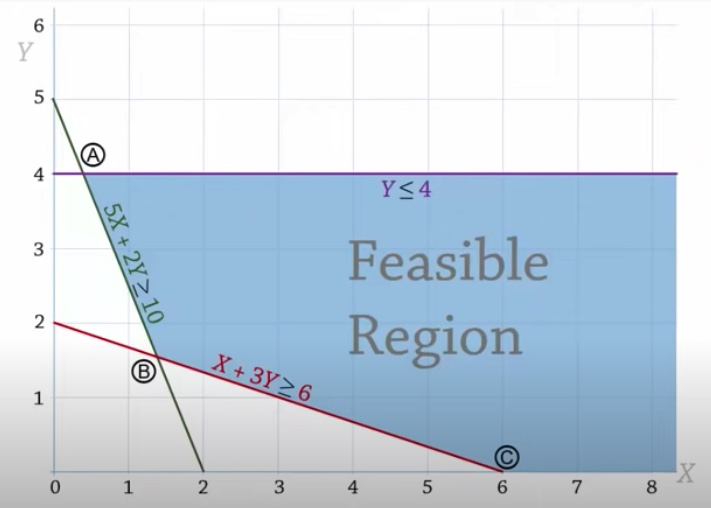
\includegraphics[scale = 0.4]{screenshots/example1-feasible-region}
\end{center}

As you can see, the feasible region is \emph{unbounded}.  In particular, from any point in the feasible region, one can always find another feasible point by increasing the $X$ coordinate (i.e., move to the right in the picture).   However, this does not necessarily mean that the optimization problem is unbounded.

Indeed, the optimal solution is at the B, the extreme point in the lower left hand corner.

\todo[inline]{To do: add contours to plot to show extreme point is the optimal solution.}

\begin{center}
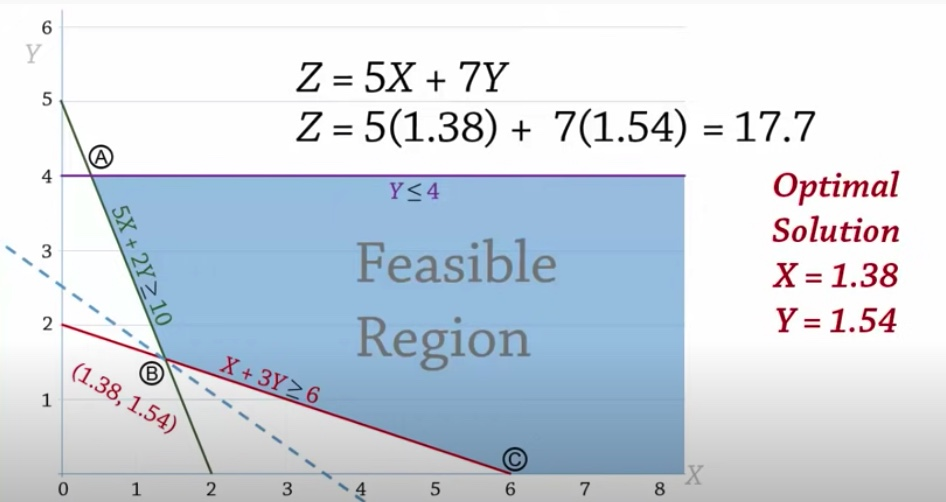
\includegraphics[scale = 0.4]{screenshots/example1-optimal-solution}
\end{center}


Consider however, if we consider a different problem where we try to maximize the objective
\begin{align*}
\max \quad & Z = 5X + 7Y\\ 
\text { s.t. } \quad & X+3 Y \geq 6 \\ 
&5 X+ 2 Y \geq 10 \\ 
&Y  \leq 4 \\ 
&X, Y  \geq 0 
\end{align*}

\begin{solution}
This optimization problem is unbounded!  For example, notice that the point $(X,Y) = (n,0)$ is feasible for all $n=1,2,3,\dots,$.   Then the objective function $Z = 5n + 0$ follows the sequence $5, 10, 15, \dots,$, which diverges to infinity.   
\end{solution}


Again, we'll tackle the issue of linear programming problems with unbounded feasible regions by illustrating the possible outcomes using examples.

\begin{example}{}{} Consider the linear programming problem below:
\begin{equation}
\left\{
\begin{aligned}
\max\;\;& z(x_1,x_2) = 2x_1 - x_2\\
s.t.\;\;& x_1 - x_2 \leq 1\\
& 2x_1 + x_2 \geq 6\\
&x_1,x_2 \geq 0
\end{aligned}
\right.
\label{eqn:LPUnboundFeasibleRegion1}
\end{equation}
\end{example}
\begin{solution}
The feasible region and level curves of the objective function are shown in Figure \ref{fig:LPUnboundFeasibleRegion1}. 
\begin{figure}[H]%[htbp]
\centering
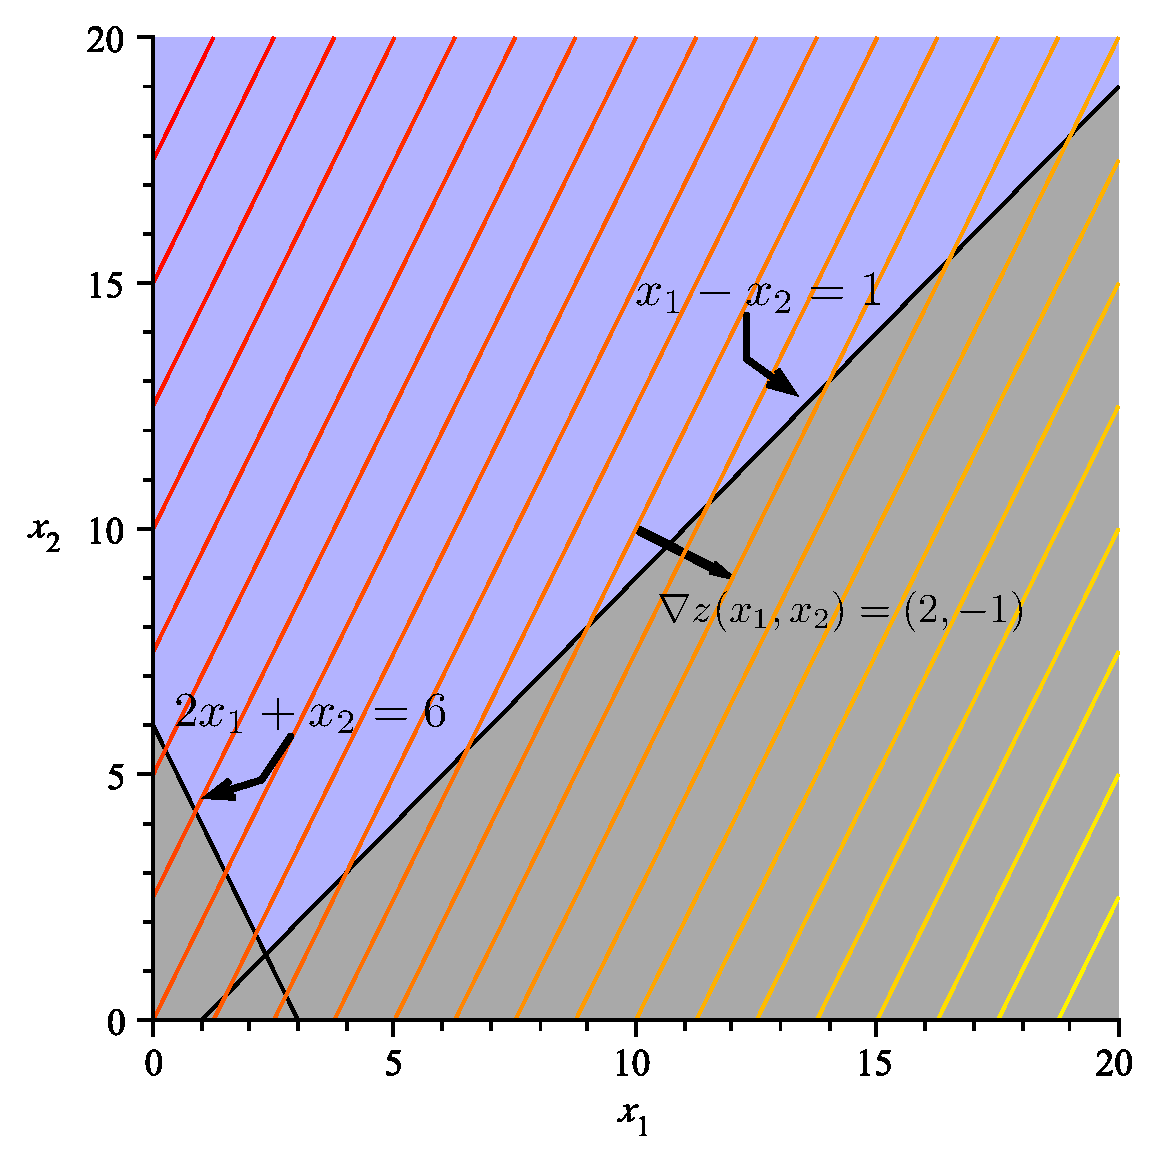
\includegraphics[scale=0.4]{UnboundedFeasibleRegion.pdf}
\caption{A Linear Programming Problem with Unbounded Feasible Region: Note that we can continue to make level curves of $z(x_1,x_2)$ corresponding to larger and larger values as we move down and to the right. These curves will continue to intersect the feasible region for any value of $v = z(x_1,x_2)$ we choose. Thus, we can make $z(x_1,x_2)$ as large as we want and still find a point in the feasible region that will provide this value. Hence, the optimal value of $z(x_1,x_2)$ subject to the constraints $+\infty$. That is, the problem is unbounded.}
\label{fig:LPUnboundFeasibleRegion1}
\end{figure}
The feasible region in Figure \ref{fig:LPUnboundFeasibleRegion1} is clearly unbounded since it stretches upward along the $x_2$ axis infinitely far and also stretches rightward along the $x_1$ axis infinitely far, bounded below by the line $x_1-x_2 = 1$. There is no way to enclose this region by a disk of finite radius, hence the feasible region is not bounded. 

We can draw more level curves of $z(x_1,x_2)$  in the direction of increase (down and to the right) as long as we wish. There will always be an intersection point with the feasible region because it is infinite. That is, these curves will continue to intersect the feasible region for any value of $v = z(x_1,x_2)$ we choose. Thus, we can make $z(x_1,x_2)$ as large as we want and still find a point in the feasible region that will provide this value. Hence, the largest value $z(x_1,x_2)$ can take when $(x_1,x_2)$ are in the feasible region is $+\infty$. That is, the problem is unbounded.
\label{ex:LPUnboundFeasibleRegion1}
\end{solution}

Just because a linear programming problem has an unbounded feasible region does not imply that there is not a finite solution. We illustrate this case by modifying example \ref{ex:LPUnboundFeasibleRegion1}. 

\begin{example}{Continuation of Example \ref{ex:LPUnboundFeasibleRegion1}}{ex:LPUnboundFeasibleRegion2}
Consider the linear programming problem from Example \ref{ex:LPUnboundFeasibleRegion1} with the new objective function: $z(x_1,x_2) = (1/2)x_1 - x_2$. Then we have the new problem:
\begin{equation}
\left\{
\begin{aligned}
\max\;\;& z(x_1,x_2) =\frac{1}{2}x_1 - x_2\\
s.t.\;\;& x_1 - x_2 \leq 1\\
& 2x_1 + x_2 \geq 6\\
&x_1,x_2 \geq 0
\end{aligned}
\right.
\label{eqn:LPUnboundFeasibleRegion2}
\end{equation}
\end{example}
\begin{solution}
The feasible region, level sets of $z(x_1,x_2)$ and gradients are shown in Figure \ref{fig:LPUnboundFeasibleRegion2}. In this case note, that the direction of increase of the objective function is \textit{away} from the direction in which the feasible region is unbounded (i.e., downward). As a result, the point in the feasible region with the largest $z(x_1,x_2)$ value is $(7/3,4/3)$. Again this is a vertex: the binding constraints are $x_1 - x_2 = 1$ and $2x_1 + x_2 = 6$ and the solution occurs at the point these two lines intersect.
\begin{figure}[H]%[htbp]
\centering
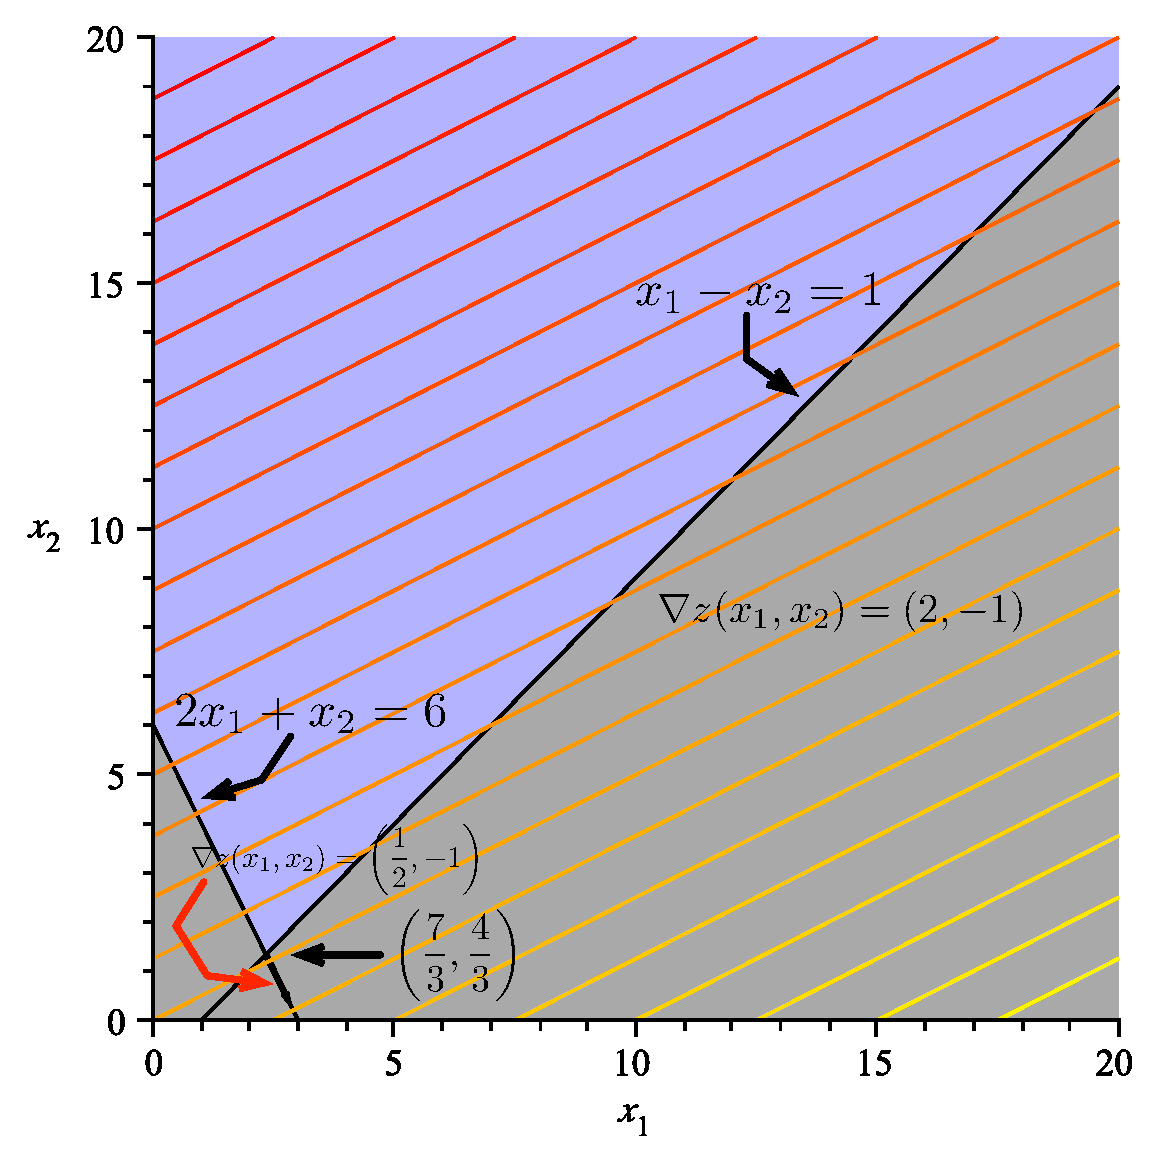
\includegraphics[scale=0.4]{UnboundedFeasibleRegionFiniteSolution.pdf}
\caption{A Linear Programming Problem with Unbounded Feasible Region and Finite Solution: In this problem, the level curves of $z(x_1,x_2)$ increase in a more ``southernly'' direction that in Example \ref{ex:LPUnboundFeasibleRegion2}--that is, \textit{away} from the direction in which the feasible region increases without bound. The point in the feasible region with largest $z(x_1,x_2)$ value is $(7/3,4/3)$. Note again, this is a vertex.}
\label{fig:LPUnboundFeasibleRegion2}
\end{figure}
\label{ex:LPUnboundFeasibleRegion2}
\end{solution}
Based on these two examples, we can modify our algorithm for graphically solving a two variable linear programming problems to deal with the case when the feasible region is unbounded.
\begin{algorithm}
\caption{Algorithm for Solving a Linear Programming Problem Graphically--Bounded and Unbounded Case}
\label{alg:GraphLPAlmostGeneral}
\begin{center}
\begin{minipage}[t]{\textwidth-1em}
\underline{\textbf{Algorithm for Solving a Two Variable Linear Programming Problem Graphically}}
\begin{enumerate*}
\item Plot the feasible region defined by the constraints.
\item If the feasible region is empty, then no solution exists.
\item If the feasible region is unbounded goto Line 8. Otherwise, Goto Line 4.
\item Plot the level sets of the objective function.
\item For a maximization problem, identify the level set corresponding the greatest (least, for minimization) objective function value that intersects the feasible region. This point will be at a corner. 
\item The point on the corner intersecting the greatest (least) level set is a solution to the linear programming problem. 
\item \textbf{If the level set corresponding to the greatest (least) objective function value is parallel to a side of the polygon boundary next to the corner identified, then there are infinitely many alternative optimal solutions and any point on this side may be chosen as an optimal solution.} 
\item (The feasible region is unbounded): Plot the level sets of the objective function.
\item If the level sets intersect the feasible region at larger and larger (smaller and smaller for a minimization problem), then the problem is unbounded and the solution is $+\infty$ ($-\infty$ for minimization problems). 
\item Otherwise, identify the level set corresponding the greatest (least, for minimization) objective function value that intersects the feasible region. This point will be at a corner. 
\item The point on the corner intersecting the greatest (least) level set is a solution to the linear programming problem. 
\textbf{If the level set corresponding to the greatest (least) objective function value is parallel to a side of the polygon boundary next to the corner identified, then there are infinitely many alternative optimal solutions and any point on this side may be chosen as an optimal solution.} 
\end{enumerate*}
\end{minipage}
\end{center}
\end{algorithm}

\begin{exercise}{}{} Does the following problem have a bounded solution? Why?
\begin{equation}
\left\{
\begin{aligned}
\boldsymbol{\min}\;\;& z(x_1,x_2) = 2x_1 - x_2\\
s.t.\;\;& x_1 - x_2 \leq 1\\
& 2x_1 + x_2 \geq 6\\
&x_1,x_2 \geq 0
\end{aligned}
\right.
\end{equation}
[Hint: Use Figure \ref{fig:LPUnboundFeasibleRegion2} and Algorithm \ref{alg:GraphLPAlmostGeneral}.]
\label{exer:BoundedSolutionQuestion}
\end{exercise}

\begin{exercise}{}{} Modify the objective function in Example \ref{ex:LPUnboundFeasibleRegion1} or Example \ref{ex:LPUnboundFeasibleRegion2} to produce a problem with an infinite number of solutions. 
\end{exercise}

\begin{exercise}{}{} Modify the objective function in Exercise \ref{exer:BoundedSolutionQuestion} to produce a \textbf{minimization} problem that has a finite solution. Draw the feasible region and level curves of the objective to ``prove'' your example works. 

\emph{[Hint: Think about what direction of increase is required for the level sets of $z(x_1,x_2)$ (or find a trick using Exercise \ref{exer:MinForMax}).]}
\end{exercise}

\section{Formal Mathematical Statements}
\todoSection{ 20\% complete. Goal 80\% completion date: July 20\\
Notes: Need to work on this section.}
\underline{\bf Vectors and Linear and Convex Combinations} \\

{\bf Vectors:} Vector $\bf n$ has ${n}$-elements and represents a point (or an arrow from the origin to the point, denoting a direction) in $\mathcal{R}^n$ space (Euclidean or real space). Vectors can be expressed as either row or column vectors. \vspace{-2mm}
\begin{description}
\item[Vector Addition:] Two vectors of the same size can be added, componentwise, e.g., for vectors
$\mathbf{a}=(2,3)$ and $\mathbf{b} = (3,2)$,  $\mathbf{a} + \mathbf{b} = (2+3,3+2) = (5,5)$. \vspace{-2mm}
\item[Scalar Multiplication:] A vector can be multiplied by a scalar $k$ (constant) component-wise. If $k > 0$ then this does not change the direction represented by the vector, it just scales the vector. \vspace{-2mm}
\item[Inner or Dot Product:] Two vectors of the same size can be multiplied to produce a real number.  For example, $\mathbf{a}\mathbf{b} = 2*3 + 3*2 = 10$.
\end{description} 

\bigskip{\bf Linear Combination:}  The vector ${\mathbf b}$ is a {\bf linear combination} of ${\mathbf a_1}, {\mathbf a_2}, \cdots, {\mathbf a_k}$ if ${\mathbf b} = \sum_{i=1}^k \lambda_i {\mathbf a_i}$ for $\lambda_1, \lambda_2,\cdots, \lambda_k \in \mathcal{R}$. If $\lambda_1, \lambda_2,\cdots,\lambda_k \in \mathcal{R}_{\ge 0}$ then ${\mathbf b}$ is a {\it non-negative linear combination} of ${\mathbf a_1},{\mathbf a_2},\cdots,{\mathbf a_k}$. \\

{\bf Convex Combination:}  The vector ${\mathbf b}$ is a {\bf convex combination} of ${\mathbf a_1},{\mathbf a_2},\cdots,{\mathbf a_k}$ if ${\mathbf b} = \sum_{i=1}^k \lambda_i {\mathbf a_i}$, for $\lambda_1, \lambda_2,\cdots,\lambda_k \in \mathcal{R}_{\ge 0}$ and $\sum_{i=1}^k \lambda_i = 1$ . For example, any convex combination of two points will lie on the line segment between the points. \\

{\bf Linear Independence:}  Vectors ${\mathbf a_1},{\mathbf a_2},\cdots,{\mathbf a_k}$ are {\it linearly independent} if the following linear combination $\sum_{i=1}^k \lambda_i {\mathbf a_i} = {\mathbf 0}$ implies that $\lambda_i = 0,~ i = 1,2,\cdots,k$. In $\mathcal{R}^2$ two vectors are only linearly dependent if they lie on the same line. Can you have three linearly independent vectors in $\mathcal{R}^2$? \\

%\bigskip {\bf Example~1} determine if the vectors $[1, 2]$ and $[-1, 1]$ are linearly independent.

%\bigskip {\bf Example~2} determine if the vectors $[1, 2, 3]$, $[-1, 1, 1]$, and $[0, 3, 2]$ are linearly independent.

%\bigskip To span $\mathrm{R^m}$ a linear combination of the vectors $\mathbf{a_i},~i=1,\cdots,m$, must be able to represent any vector in $\mathrm{R^m}$, i.e., $\sum_{i=1}^m\lambda_i\mathbf{a_i}$ can represent any vector in $\mathrm{R^m}$ by appropriately setting the $\lambda$'s. A set of vectors is a {\it basis} in $\mathrm{R^m}$ if they span $\mathrm{R^m}$ and removing any vector from the set leaves a set that does not span $\mathrm{R^m}$, in this case, $m$ linearly independent vectors (i.e., if $\sum_{i=1}^k\lambda_i\mathbf{a_i} = \mathbf{0}$ can only occur if $\lambda_i=0$ for all $i=1,\cdots,j$) form a basis and are a minimum spanning set.

{\bf Spanning Set:}  Vectors ${\mathbf a_1},{\mathbf a_2},\cdots,{\mathbf a_k}$ span $\mathcal{R}^m$ is any vector in $\mathcal{R}^m$ can be represented as a linear combination of ${\mathbf a_1},{\mathbf a_2},\cdots,{\mathbf a_k}$, i.e., $\sum_{i=1}^m\lambda_i\mathbf{a_i}$ can represent any vector in $\mathcal{R}^m$. \\

{\bf Basis:} Vectors ${\mathbf a_1},{\mathbf a_2},\cdots,{\mathbf a_k}$ form a basis of $\mathcal{R}^m$ if they span $\mathcal{R}^m$ and any smaller subset of these vectors does not span $\mathcal{R}^m$. Vectors ${\mathbf a_1},{\mathbf a_2},\cdots,{\mathbf a_k}$ can only form a basis of $\mathcal{R}^m$ if $k = m$ and they are linearly independent.

\newpage \underline{\bf Convex and Polyhedral Sets} \\

{\bf Convex Set:} Set $\mathcal{S}$ in $\mathcal{R}^n$ is a {\it convex set} if a line segment joining any pair of points $\mathbf{a_1}$ and $\mathbf{a_2}$ in $\mathcal{S}$ is completely contained in $\mathcal{s}$, that is, $\lambda\mathbf{a_1} + (1-\lambda)\mathbf{a_2} \in \mathcal{S}, \forall \lambda \in [0,1]$. \\

{\bf Hyperplanes and Half-Spaces:} A hyperplane in $\mathcal{R}^n$ divides $\mathcal{R}^n$ into 2 half-spaces (like a line does in $\mathcal{R}^2$). A hyperplane is the set $\{\mathbf{x}: \mathbf{p}\mathbf{x} = k\}$, where $\mathbf{p}$ is the gradient to the hyperplane (i.e., the coefficients of our linear expression). The corresponding half-spaces is the set of points $\{\mathbf{x}: \mathbf{p}\mathbf{x} \ge k\}$ and $\{\mathbf{x}: \mathbf{p}\mathbf{x} \le k\}$. \\

{\bf Polyhedral Set:} A {\it polyhedral set} (or polyhedron) is the set of points in the intersection of a finite set of half-spaces. Set $\mathcal{S} = \{\mathbf{x}: \mathbf{A} \mathbf{x} \le \mathbf{b}, \mathbf{x} \ge \mathbf{0}\}$, where $\mathbf{A}$ is an $m \times n$ matrix, $\mathbf{x}$ is an $n$-vector, and $\mathbf{b}$ is an $m$-vector, is a {\it polyhedral set} defined by $m + n$ hyperplanes (i.e., the intersection of $m + n$ half-spaces).
\begin{itemize}
\item Polyhedral sets are convex. 
\item A polytope is a bounded polyhedral set.
\item A polyhedral cone is a polyhedral set where the hyperplanes (that define the half-spaces) pass through the origin, thus $\mathcal{C} = \{\mathbf{x}: \mathbf{A} \mathbf{x} \le \mathbf{0}\}$ is a polyhedral cone.
\end{itemize}

{\bf Edges and Faces:} An {\it edge} of a polyhedral set $\mathcal{S}$ is defined by $n-1$ hyperplanes, and a {\it face} of $\mathcal{S}$ by one of more defining hyperplanes of $\mathcal{S}$, thus an extreme point and an edge are faces (an extreme point is a zero-dimensional face and an edge a one-dimensional face).  In $\mathcal{R}^2$ faces are only edges and extreme points, but in $\mathcal{R}^3$ there is a third type of face, and so on... \\

{\bf Extreme Points:} $\mathbf{x} \in \mathcal{S}$ is an extreme point of $\mathcal{S}$ if:
\begin{description}
\item[Definition 1:] $\mathbf{x}$ is not a convex combination of two other points in $\mathcal{S}$, that is, all line segments that are completely in $\mathcal{S}$ that contain $\mathbf{x}$ must have $\mathbf{x}$ as an endpoint.
\item[Definition 2:] $\mathbf{x}$ lies on $n$ linearly independent defining hyperplanes of $\mathcal{S}$.
\end{description}


If more than $n$ hyperplanes pass through an extreme points then it is a degenerate extreme point, and the polyhedral set is considered degenerate. This just adds a bit of complexity to the algorithms we will study, but it is quite common. \\
  

\underline {\bf Unbounded Sets:} \\ 

{\bf Rays:} A ray in $\mathcal{R}^n$ is the set of points $\{\mathbf{x}: \mathbf{x_0} + \lambda\mathbf{d},~ \lambda \ge 0\}$, where $\mathbf{x_0}$ is the vertex and $\mathbf{d}$ is the direction of the ray.\\


{\bf Convex Cone:} A {\it Convex Cone} is a convex set that consists of rays emanating from the origin.  A convex cone is completely specified by its extreme directions.  If $\mathcal{C}$ is convex cone, then for any $\mathbf{x} \in \mathcal{C}$ we have $\lambda \mathbf{x} \in \mathcal{C},~ \lambda \ge 0$. \\

{\bf Unbounded Polyhedral Sets:} If $\mathcal{S}$ is unbounded, it will have {\it directions}. $\mathbf{d}$ is a direction of $\mathcal{S}$ only if $\mathbf{A} \mathbf{x} + \lambda\mathbf{d} \le \mathbf{b}, \mathbf{x} + \lambda\mathbf{d} \ge \mathbf{0}$ for all $\lambda \ge 0$ and all $\mathbf{x} \in \mathcal{S}$.  In other words, consider the ray $\{\mathbf{x}: \mathbf{x_0} + \lambda\mathbf{d},~ \lambda \ge 0\}$ in $\mathcal{R}^n$, where $\mathbf{x_0}$ is the vertex and $\mathbf{d}$ is the direction of the ray. $\mathbf{d} \ne \mathbf{0}$ is a {\bf direction} of set $\mathcal{S}$ if for each $\mathbf{x_0}$ in $\mathcal{S}$ the ray $\{\mathbf{x_0} + \lambda\mathbf{d},~ \lambda \ge 0\}$ also belongs to $\mathcal{S}$. \\

{\bf Extreme Directions:} An {\it extreme direction} of $\mathcal{S}$ is a direction that {\it cannot} be represented as positive linear combination of other directions of $\mathcal{S}$. A non-negative linear combination of extreme directions can be used to represent all other directions of $\mathcal{S}$. A polyhedral cone is completely specified by its extreme directions. \\

Let's define a procedure for finding the extreme directions, using the following LP's feasible region.  Graphically, we can see that the extreme directions should follow the the $s_1=0$ (red) line and the $s_3 = 0$ (orange) line. 
 
\begin{minipage}[t][][b]{.4\linewidth}
\begin{align*}
\mbox{max~~} & z = -5x_1 - x_2  \\\
\mbox{s.t.~~} & x_1 - 4x_2 +s_1 = 0  \\
& -x_1 + x_2 + s_2 = 1 \\
& -x_1 + 2x_2 +s_3 = 4 \\
& x_1, x_2, s_1, s_2, s_3 \ge 0.
\end{align*}
\end{minipage}%
\begin{minipage}[t][][b]{.6\linewidth}
\begin{center}  \begin{tikzpicture} [scale=1.5]
    \draw[gray!50, thin, step=.5] (0,0) grid (5,5);
    \draw[opacity=0.9] (0,0) -- (5.4,0) node[below] {$x_1$};
    \draw[opacity=0.9] (0,0) -- (0,5.4) node[left] {$x_2$}; % option \draw[very thick,->]

    \foreach \x in {0,...,5} \draw (\x,0.05) -- (\x,-0.05) node[below] {\x};
    \foreach \y in {0,...,5} \draw (-0.05,\y) -- (0.05,\y) node[left] {\y};

    \fill[yellow,opacity=0.3] (0,0) -- (0,1) -- (2,3) -- (5,4.5) --(5,1.25)-- cycle;

    \draw [red](0,0) -- node[below] {$s_1=0$} (5, 1.25);
    \draw [teal] (0,1)  --  (4,5) node[left, sloped] {$s_2=0$};
    \draw [orange](0,2) --  (5,4.5) node[below, sloped] {$s_3=0$}; %node[above right ,sloped] 
	\filldraw[fill=red] (-0.05,-0.05) rectangle (0.05,0.05);
	\filldraw[fill=red] (-0.05,.95) rectangle (0.05,1.05);
	\filldraw[fill=red] (1.95,2.95) rectangle (2.05,3.05);
\end{tikzpicture} \end{center} 
\end{minipage}

\begin{center}  \begin{tikzpicture} [scale=1.5]
    \draw[gray!50, thin, step=.5] (0,0) grid (5,5);
    \draw[opacity=0.9] (0,0) -- (5.4,0) node[below] {$x_1$};
    \draw[opacity=0.9] (0,0) -- (0,5.4) node[left] {$x_2$}; % option \draw[very thick,->]

    \foreach \x in {0,...,5} \draw (\x,0.05) -- (\x,-0.05) node[below] {\x};
    \foreach \y in {0,...,5} \draw (-0.05,\y) -- (0.05,\y) node[left] {\y};

    \fill[yellow,opacity=0.3] (0,0) -- (0,1) -- (2,3) -- (5,4.5) --(5,1.25)-- cycle;

\draw[domain=0:4,smooth,variable=\x, teal] plot ({\x},{\x+1}) node[left] {$s_2=0$};
\draw[domain=0:5,smooth,variable=\x, red] plot ({\x},{\x*1/4}) node[below] {$s_1=0$};
%    \draw [red](0,0) -- node[below] {$s_1=0$} (5, 1.25);
    %\draw [teal] (0,1)  --  (4,5) node[left, sloped] {$s_2=0$};
    \draw [orange](0,2) --  (5,4.5) node[below, sloped] {$s_3=0$}; %node[above right ,sloped] 
	\filldraw[fill=red] (-0.05,-0.05) rectangle (0.05,0.05);
	\filldraw[fill=red] (-0.05,.95) rectangle (0.05,1.05);
	\filldraw[fill=red] (1.95,2.95) rectangle (2.05,3.05);
\end{tikzpicture} \end{center} 

% \draw[scale=0.5,domain=-3:3,smooth,variable=\x,blue] plot ({\x},{\x*\x});


\medskip E.g., consider the $s_3=0$ (orange) line, to find the extreme direction start at extreme point (2,3) and find another feasible point on the orange line, say (4,4) and subtract (2,3) from (4,4), which yields (2,1). 

\medskip This is related to the slope in two-dimensions, as discussed in class, the rise is 1 and the run is 2. So this direction has a slope of 1/2, but this does not carry over easily to higher dimensions where directions cannot be defined by a single number. 

\medskip To find the extreme directions we can change the right-hand-side to $\mathbf{b} = \mathbf{0}$, which forms a polyhedral cone (in yellow), and then add the constraint $x_1 + x_2 = 1$. The intersection of the cone and  $x_1 + x_2 = 1$ form a line segment.

\begin{minipage}[t][][b]{.4\linewidth} \vspace{0mm}
\begin{align*}
\mbox{max~~} & z = -5x_1 - x_2  \\
\mbox{s.t.~~} & x_1 - 4x_2 +s_1 = 0  \\
& -x_1 + x_2 + s_2 = 0 \\
& -x_1 + 2x_2 +s_3 = 0 \\
& x_1 + x_2 = 1 \\
& x_1, x_2, s_1, s_2, s_3 \ge 0.
\end{align*}
\end{minipage}%
\begin{minipage}[t][][b]{.6\linewidth}
\begin{center} \begin{tikzpicture} [scale=1.5]
\draw[gray!50, thin, step=.5] (0,0) grid (4,4);
\draw[opacity=0.9] (0,0) -- (4.4,0) node[below] {$x_1$};
\draw[opacity=0.9] (0,0) -- (0,4.4) node[left] {$x_2$}; % option \draw[very thick,->]

\foreach \x in {0,...,4} \draw (\x,0.05) -- (\x,-0.05) node[below] {\x};
\foreach \y in {0,...,4} \draw (-0.05,\y) -- (0.05,\y) node[left] {\y};
        
\draw [red](0, 0) -- node[below] {$s_1=0$} (4, 1);
\draw [teal] (0,0)  -- (4,4) node[left, sloped] {$s_2=0$};
\draw [orange](0,0) -- (4,2) node[below, sloped] {$s_3=0$}; 
\fill[yellow,opacity=0.3] (0,0) -- (4,2) -- (4,1) --  cycle; % \draw [orange!50!blue] 

\draw [black] (0,1)  -- node[above right] {$x_1+x_2 = 1$} (1,0); 
\end{tikzpicture} \end{center} 
\end{minipage}



\begin{center} \begin{tikzpicture} [scale=1.5]
\draw[gray!50, thin, step=.5] (0,0) grid (4,4);
\draw[opacity=0.9] (0,0) -- (4.4,0) node[below] {$x_1$};
\draw[opacity=0.9] (0,0) -- (0,4.4) node[left] {$x_2$}; % option \draw[very thick,->]

\foreach \x in {0,...,4} \draw (\x,0.05) -- (\x,-0.05) node[below] {\x};
\foreach \y in {0,...,4} \draw (-0.05,\y) -- (0.05,\y) node[left] {\y};
        
\draw [red](0, 0) -- node[below] {$s_1=0$} (4, 1);
\draw [teal] (0,0)  -- (4,4) node[left, sloped] {$s_2=0$};
\draw [orange](0,0) -- (4,2) node[below, sloped] {$s_3=0$}; 
\fill[yellow,opacity=0.3] (0,0) -- (4,2) -- (4,1) --  cycle; % \draw [orange!50!blue] 

\draw [black] (0,1)  -- node[above right] {$x_1+x_2 = 1$} (1,0); 
\end{tikzpicture} \end{center} 


\medskip Magnifying for clarity, and removing the $s_2=0$ (teal) line, as it is redundant, and marking the extreme points of the new feasible region, (4/5, 1/5) and (2/3, 1/3), with red boxes, we have:

\begin{center}  \begin{tikzpicture} [x=50mm, y=50mm] [scale=1.5]
\draw[gray!50, thin, step=.5] (0,0) grid (2,1);
\draw[opacity=0.9] (0,0) -- (2.2,0) node[below] {$x_1$};
\draw[opacity=0.9] (0,0) -- (0,1.2) node[left] {$x_2$}; % option \draw[very thick,->]

\foreach \x in {0,...,2} \draw (\x,0.005) -- (\x,-0.005) node[below] {\x};
\foreach \y in {0,...,1} \draw (-0.005,\y) -- (0.005,\y) node[left] {\y};

\filldraw[fill=red] (0.8-0.02,0.2-0.02) rectangle (0.8+0.02,0.2+0.02);
\filldraw[fill=red] (0.667-0.02,0.333-0.02) rectangle (0.667+0.02,0.333+0.02);

\draw [red](0, 0) -- node[below] {$s_1=0$} (2, .5);
\draw [orange](0,0) -- (2,1) node[below, sloped] {$s_3=0$}; 
\fill[yellow,opacity=0.3] (0,0) -- (2,.5) -- (2,1) --  cycle; % \draw [orange!50!blue] 
\draw [black] (0,1)  -- node[above right] {$x_1+x_2 = 1$} (1,0); 
\end{tikzpicture} \end{center} 

The extreme directions are thus (4/5, 1/5) and (2/3, 1/3). \\

{\bf Representation Theorem:} Let  $\mathbf{x_1}, \mathbf{x_2},\cdots \mathbf{x_k}$ be the set of extreme points of $\mathcal{S}$, and if $\mathcal{S}$ is unbounded, $\mathbf{d_1}, \mathbf{d_2},\cdots \mathbf{d_l}$ be the set of extreme directions. Then any $\mathbf{x} \in \mathcal{S}$ is equal to a convex combination of the extreme points and a non-negative linear combination of the extreme directions: $\mathbf{x} = \sum_{j=1}^k \lambda_j \mathbf{x_j} + \sum_{j=1}^l \mu_j \mathbf{d_j}$, where $\sum_{j=1}^k \lambda_j = 1$, $\lambda_j \ge 0,~\forall  j=1,2,\cdots,k$, and $\mu_j \ge 0,~\forall j=1,2,\cdots,l$.

 \begin{minipage}[t][][b]{.4\linewidth}
\begin{align*}
\mbox{max~~} & z = -5x_1 - x_2  \\\
\mbox{s.t.~~} & x_1 - 4x_2 +s_1 = 0  \\
& -x_1 + x_2 + s_2 = 1 \\
& -x_1 + 2x_2 +s_3 = 4 \\
& x_1, x_2, s_1, s_2, s_3 \ge 0.
\end{align*}
\end{minipage}%
\begin{minipage}[t][][b]{.6\linewidth}
\begin{center}  \begin{tikzpicture} [scale=1.5]
    \draw[gray!50, thin, step=.5] (0,0) grid (5,5);
    \draw[opacity=0.9] (0,0) -- (5.4,0) node[below] {$x_1$};
    \draw[opacity=0.9] (0,0) -- (0,5.4) node[left] {$x_2$}; % option \draw[very thick,->]

    \foreach \x in {0,...,5} \draw (\x,0.05) -- (\x,-0.05) node[below] {\x};
    \foreach \y in {0,...,5} \draw (-0.05,\y) -- (0.05,\y) node[left] {\y};

    \fill[yellow,opacity=0.3] (0,0) -- (0,1) -- (2,3) -- (5,4.5) --(5,1.25)-- cycle;

    \draw [red](0,0) -- node[below] {$s_1=0$} (5, 1.25);
    \draw [teal] (0,1)  --  (4,5) node[left, sloped] {$s_2=0$};
    \draw [orange](0,2) --  (5,4.5) node[below, sloped] {$s_3=0$}; %node[above right ,sloped] 
	\filldraw[fill=red] (-0.05,-0.05) rectangle (0.05,0.05);
	\filldraw[fill=red] (-0.05,.95) rectangle (0.05,1.05);
	\filldraw[fill=red] (1.95,2.95) rectangle (2.05,3.05);
\end{tikzpicture} \end{center} 
\end{minipage}

Represent point (1/2, 1) as a convex combination of the extreme points of the above LP.  Find $\lambda$s to solve the following system of equations:

$$\lambda_1 \left[
  \begin{array}{c}
  0 \\
  0 \\
  \end{array} \right]+
 \lambda_2 \left[
  \begin{array}{c}
  0 \\
  1 \\
  \end{array} \right] +
 \lambda_3 \left[
  \begin{array}{c}
  2 \\
  3 \\
  \end{array} \right]  =
 \left[
  \begin{array}{c}
  1/2 \\
  1 \\
  \end{array} \right] 
$$




\chapter{Matrices, Linear Algebra and Linear Programming}\label{chap:Matrices}
In this section, we will review matrix concepts critical for the general understanding of general linear programming algorithms. 

Let $\mathbf{x}$ and $\mathbf{y}$ be two vectors in $\mathbb{R}^n$. Recall we denote the dot product of the two vectors as $\mathbf{x} \cdot \mathbf{y}$. 

\section{Matrices}
Recall an $m \times n$ matrix is a rectangular array of numbers, usually drawn from a field such as $\mathbb{R}$. We write an $m \times n$ matrix with values in $\mathbb{R}$ as $\mathbf{A} \in \mathbb{R}^{m \times n}$. The matrix consists of $m$ rows and $n$ columns. The element in the $i^\text{th}$ row and $j^\text{th}$ column of $\mathbf{A}$ is written as $\mathbf{A}_{ij}$. The $j^\text{th}$ column of $\mathbf{A}$ can be written as $\mathbf{A}_{\cdot j}$, where the $\cdot$ is interpreted as ranging over every value of $i$ (from $1$ to $m$). Similarly, the $i^{th}$ row of $\mathbf{A}$ can be written as $\mathbf{A}_{i\cdot}$. When $m = n$, then the matrix $\mathbf{A}$ is called \textit{square}.

\begin{definition}[Matrix Addition]
If $\mathbf{A}$ and $\mathbf{B}$ are both in $\mathbb{R}^{m \times n}$, then $\mathbf{C} = \mathbf{A} + \mathbf{B}$ is the matrix sum of $\mathbf{A}$ and $\mathbf{B}$ and 
\begin{equation}
\mathbf{C}_{ij} = \mathbf{A}_{ij} + \mathbf{B}_{ij}\;\; \text{for $i=1,\dots,m$ and $j=1,\dots,n$}
\end{equation}
\end{definition}

\begin{example} 
\begin{equation}
\left[
\begin{array}{cc}
1 & 2\\
3 & 4
\end{array}
\right] + 
\left[
\begin{array}{cc}
5 & 6\\
7 & 8
\end{array}
\right] = 
\left[
\begin{array}{cc}
1 + 5 & 2 + 6\\
3 + 7 & 4 + 8
\end{array}
\right] = 
\left[
\begin{array}{cc}
6 & 8\\
10 & 12
\end{array}
\right]
\end{equation}
\end{example}

\begin{definition}[Row/Column Vector]
A $1 \times n$ matrix is called a \textit{row vector}, and a $m \times 1$ matrix is called a \textit{column vector}. For the remainder of these notes, every vector will be thought of \textbf{column vector} unless otherwise noted.
\end{definition}

It should be clear that any row of matrix $\mathbf{A}$ could be considered a row vector in $\mathbb{R}^n$ and any column of $\mathbf{A}$ could be considered a column vector in $\mathbb{R}^m$.

\begin{definition}[Matrix Multiplication]
If $\mathbf{A} \in \mathbb{R}^{m \times n}$ and $B \in \mathbb{R}^{n \times p}$, then $\mathbf{C} = \mathbf{A}\mathbf{B}$ is the \textit{matrix product} of $\mathbf{A}$ and $\mathbf{B}$ and
\begin{equation}
\mathbf{C}_{ij} = \mathbf{A}_{i\cdot} \cdot \mathbf{B}_{\cdot j}
\end{equation}
Note, $\mathbf{A}_{i\cdot} \in \mathbb{R}^{1 \times n}$ (an $n$-dimensional vector) and $\mathbf{B}_{\cdot j} \in \mathbb{R}^{n \times 1}$ (another $n$-dimensional vector), thus making the dot product meaningful. 
\end{definition}

\begin{example} 
\begin{equation}
\left[
\begin{array}{cc}
1 & 2\\
3 & 4
\end{array}
\right] 
\left[
\begin{array}{cc}
5 & 6\\
7 & 8
\end{array}
\right] = 
\left[
\begin{array}{cc}
1(5) + 2(7) & 1(6) + 2(8)\\
3(5) + 4(7) & 3(6) + 4(8)
\end{array}
\right] = 
\left[
\begin{array}{cc}
19 & 22\\
43 & 50
\end{array}
\right]
\end{equation}
\end{example}

\begin{definition}[Matrix Transpose] If $\mathbf{A} \in \mathbb{R}^{m \times n}$ is a $m \times n$ matrix, then the \textit{transpose} of $\mathbf{A}$ dented $\mathbf{A}^T$ is an $m \times n$ matrix defined as:
\begin{equation}
\mathbf{A}^T_{ij} = \mathbf{A}_{ji}
\end{equation}
\end{definition}
\begin{example}
\begin{equation}
\left[
\begin{array}{cc}
1 & 2\\
3 & 4
\end{array}
\right]^T = 
\left[
\begin{array}{cc}
1 & 3\\
2 & 4
\end{array}
\right] 
\end{equation}
\end{example}

The matrix transpose is a particularly useful operation and makes it easy to transform column vectors into row vectors, which enables multiplication. For example, suppose $\mathbf{x}$ is an $n \times 1$ column vector (i.e., $\mathbf{x}$ is a vector in $\mathbb{R}^n$) and suppose $\mathbf{y}$ is an $n \times 1$ column vector. Then:
\begin{equation}
\mathbf{x} \cdot \mathbf{y} = \mathbf{x}^T\mathbf{y}
\end{equation}

\begin{exercise} Let $\mathbf{A}, \mathbf{B} \in \mathbb{R}^{m \times n}$. Use the definitions of matrix addition and transpose to prove that:
\begin{equation}
(\mathbf{A} + \mathbf{B})^T = \mathbf{A}^T + \mathbf{B}^T
\end{equation}
[Hint: If $\mathbf{C} = \mathbf{A} + \mathbf{B}$, then $\mathbf{C}_{ij} = \mathbf{A}_{ij} + \mathbf{B}_{ij}$, the element in the $(i,j)$ position of matrix $\mathbf{C}$. This element moves to the $(j,i)$ position in the transpose. The $(j,i)$ position of $\mathbf{A}^T + \mathbf{B}^T$ is $\mathbf{A}_{ji}^T + \mathbf{B}^T_{ji}$, but $\mathbf{A}_{ji}^T = \mathbf{A}_{ij}$. Reason from this point.] 
\label{exer:AdditionTranspose}
\end{exercise}

\begin{exercise} Let $\mathbf{A}, \mathbf{B} \in \mathbb{R}^{m \times n}$. Prove by example that $\mathbf{A}\mathbf{B} \neq \mathbf{B}\mathbf{A}$; that is, matrix multiplication is \textit{not commutative}. [Hint: Almost any pair of matrices you pick (that can be multiplied) will not commute.]
\end{exercise}

\begin{exercise} Let $\mathbf{A} \in \mathbb{R}^{m \times n}$ and let, $\mathbf{B} \in \mathbb{R}^{n \times p}$. Use the definitions of matrix multiplication and transpose to prove that:
\begin{equation}
(\mathbf{A}\mathbf{B})^T = \mathbf{B}^T\mathbf{A}^T
\end{equation}
[Hint: Use similar reasoning to the hint in Exercise \ref{exer:AdditionTranspose}. But this time, note that $\mathbf{C}_{ij} = \mathbf{A}_{i\cdot} \cdot \mathbf{B}_{\cdot j}$, which moves to the $(j,i)$ position. Now figure out what is in the $(j,i)$ position of $\mathbf{B}^T\mathbf{A}^T$.]
\end{exercise}

Let $\mathbf{A}$ and $\mathbf{B}$ be two matrices with the same number of rows (so $\mathbf{A} \in \mathbb{R}^{m \times n}$ and $\mathbf{B} \in \mathbb{R}^{m \times p}$). Then the augmented matrix $\left[\mathbf{A}|\mathbf{B}\right]$ is:
\begin{equation}
\left[
\begin{array}{cccc|cccc}
a_{11} & a_{12} & \dots & a_{1n} & b_{11} & b_{12} & \dots & b_{1p}\\
a_{21} & a_{22} & \dots & a_{2n} & b_{21} & b_{22} & \dots & b_{2p}\\
\vdots & & \ddots & \vdots & \vdots & & \ddots & \vdots\\
a_{m1} & a_{m2} & \dots & a_{mn} & b_{m1} & b_{m2} & \dots & b_{mp}\\
\end{array}
\right]
\end{equation}
Thus, $\left[\mathbf{A}|\mathbf{B}\right]$ is a matrix in $\mathbb{R}^{m \times (n + p)}$. 

\begin{example} Consider the following matrices:
\begin{displaymath}
\mathbf{A} = \left[ 
\begin{array}{cc}
1 & 2\\
3 & 4
\end{array}
\right],\;\;\;\mathbf{b} = \left[
\begin{array}{c}
7\\
8
\end{array}
\right]
\end{displaymath}
Then $\left[\mathbf{A}|\mathbf{B}\right]$ is:
\begin{displaymath}
\left[\mathbf{A}|\mathbf{B}\right] = \left[ 
\begin{array}{cc|c}
1 & 2 & 7\\
3 & 4 & 8
\end{array}
\right]
\end{displaymath}
\end{example}

\begin{exercise} By analogy define the augmented matrix $\left[\frac{\mathbf{A}}{\mathbf{B}}\right]$. Note, this is \textbf{not} a fraction. In your definition, identify the appropriate requirements on the relationship between the number of rows and columns that the matrices must have. [Hint: Unlike $\left[\mathbf{A}|\mathbf{B}\right]$, the number of rows don't have to be the same, since your concatenating on the rows, not columns. There should be a relation between the numbers of columns though.]
\end{exercise}

\section{Special Matrices and Vectors}
\begin{definition}[Identify Matrix] The $n \times n$ \textit{identify matrix} is:
\begin{equation}
\mathbf{I}_n = 
\left[
\begin{array}{cccc}
1 & 0 & \dots & 0\\
0 & 1 & \dots & 0\\
\vdots & & \ddots & \vdots\\
0 & 0 & \dots & 1
\end{array}\right]
\end{equation}
\end{definition}
When it is clear from context, we may simply write $\mathbf{I}$ and omit the subscript $n$. 
\begin{exercise} Let $\mathbf{A} \in \mathbb{R}^{n \times n}$. Show that $\mathbf{A}\mathbf{I}_n = \mathbf{I}_n\mathbf{A} = \mathbf{A}$. Hence, $\mathbf{I}$ is an identify for the matrix multiplication operation on square matrices. [Hint: Do the multiplication out long hand.]
\end{exercise}
\begin{definition}[Standard Basis Vector] The standard basis vector $\mathbf{e}_i \in \mathbb{R}^n$ is:
\begin{displaymath}
\mathbf{e}_i = \left(\underset{i-1}{\underbrace{0,0,\dots}},1,
\underset{n-i-1}{\underbrace{0,\dots,0}}\right)
\end{displaymath}
Note, this definition is only valid for $n \geq i$. Further the standard basis vector $\mathbf{e}_i$ is also the $i^{\text{th}}$ row or column of $\mathbf{I}_n$. 
\end{definition}

\begin{definition}[Unit and Zero Vectors] The vector $\mathbf{e} \in \mathbb{R}^n$ is the \textit{one vector} $\mathbf{e} = (1,1,\dots,1)$. Similarly, the \textit{zero vector} $\mathbf{0} = (0,0,\dots,0) \in \mathbb{R}^n$. We assume that the length of $\mathbf{e}$ and $\mathbf{0}$ will be determined from context. 
\end{definition}

\begin{exercise} Let $\mathbf{x} \in \mathbb{R}^n$, considered as a column vector (our standard assumption). Define:
\begin{displaymath}
\mathbf{y} = \frac{\mathbf{x}}{\mathbf{e}^T\mathbf{x}}
\end{displaymath}
Show that $\mathbf{e}^T\mathbf{y} = \mathbf{y}^T\mathbf{e} = 1$. [Hint: First remember that $\mathbf{e}^T\mathbf{x}$ is a scalar value (it's $\mathbf{e}\cdot\mathbf{x}$. Second, remember that a scalar times a vector is just a new vector with each term multiplied by the scalar. Last, use these two pieces of information to write the product $\mathbf{e}^T\mathbf{y}$ as a sum of fractions.]
\end{exercise}

\section{Matrices and Linear Programming Expression}
You will recall from your matrices class (Math 220) that matrices can be used as a short hand way to represent linear equations. Consider the following system of equations:
\begin{equation}
\left\{
\begin{aligned}
a_{11}x_1 + a_{12}x_2 + \dots + a_{1n}x_n & = b_1\\
a_{21}x_1 + a_{22}x_2 + \dots + a_{2n}x_n & = b_2\\
\vdots\\
a_{m1}x_1 + a_{m2}x_2 + \dots + a_{mn}x_n & = b_m
\end{aligned}\right.
\label{eqn:LinearEqns}
\end{equation}
Then we can write this in matrix notation as:
\begin{equation}
\mathbf{A}\mathbf{x} = \mathbf{b}
\end{equation}
where $\mathbf{A}_{ij} = a_{ij}$ for $i=1,\dots,m$, $j=1,\dots,n$ and $\mathbf{x}$ is a column vector in $\mathbb{R}^n$ with entries $x_j$ ($j=1,\dots,n$) and $\mathbf{b}$ is a column vector in $\mathbb{R}^m$ with entries $b_i$ ($i=1\dots,m$). Obviously, if we replace the equalities in Expression \ref{eqn:LinearEqns} with inequalities, we can also express systems of inequalities in the form:
\begin{equation}
\mathbf{A}\mathbf{x} \leq \mathbf{b}
\end{equation}

Using this representation, we can write our general linear programming problem using matrix and vector notation. Expression \ref{eqn:GeneralLPMax} can be written as:
\begin{equation}
\left\{
\begin{aligned}
\max\;\; z(\mathbf{x}) = &\mathbf{c}^T\mathbf{x}\\
s.t.\;\;&\mathbf{A}\mathbf{x} \leq \mathbf{b}\\
& \mathbf{H}\mathbf{x} = \mathbf{r}
\end{aligned}\right.
\label{eqn:GeneralLPMaxMatrixForm}
\end{equation}

For historical reasons, linear programs are not written in the general form of Expression \ref{eqn:GeneralLPMaxMatrixForm}. 

\begin{definition}[Canonical Form]  A maximization linear programming problem is in \textit{canonical form} if it is written as:
\begin{equation}
\left\{
\begin{aligned}
\max\;\; z(\mathbf{x}) = &\mathbf{c}^T\mathbf{x}\\
s.t.\;\;&\mathbf{A}\mathbf{x} \leq \mathbf{b}\\
& \mathbf{x} \geq \mathbf{0}
\end{aligned}\right.
\label{eqn:CanonicalFormMax}
\end{equation}

A minimization linear programming problem is in \textit{canonical form} if it is written as:
\begin{equation}
\left\{
\begin{aligned}
\min\;\; z(\mathbf{x}) = &\mathbf{c}^T\mathbf{x}\\
s.t.\;\;&\mathbf{A}\mathbf{x} \geq \mathbf{b}\\
& \mathbf{x} \geq \mathbf{0}
\end{aligned}\right.
\label{eqn:MinCanonicalFormMax}
\end{equation}
\end{definition}

\begin{definition}[Standard Form (Max Problem)]  A maximization linear programming problem is in \textit{standard form} if it is written as:
\begin{equation}
\left\{
\begin{aligned}
\max\;\; z(\mathbf{x}) = &\mathbf{c}^T\mathbf{x}\\
s.t.\;\;&\mathbf{A}\mathbf{x} = \mathbf{b}\\
& \mathbf{x} \geq \mathbf{0}
\end{aligned}\right.
\label{eqn:StandardFormMax}
\end{equation}
\end{definition}

\begin{remark} In the previous definition, a problem is in standard form as long as its constraints have form $\mathbf{A}\mathbf{x} = \mathbf{b}$ and $\mathbf{x} \geq \mathbf{0}$. The problem can be either a maximization or minimization problem.
\end{remark}


\begin{theorem}Every linear programming problem in canonical form can be put into standard form.
\end{theorem}
\begin{proof} Consider the constraint corresponding to the first row of the matrix $\mathbf{A}$:
\begin{equation}
a_{11}x_1 + a_{12}x_2 + \dots + a_{1n}x_n \leq b_1
\end{equation}
Then we can add a new \textit{slack} variable $s_1$ so that $s_1 \geq 0$ and we have:
\begin{equation}
a_{11}x_1 + a_{12}x_2 + \dots + a_{1n}x_n + s_1 = b_1
\end{equation}
This act can be repeated for each row of $\mathbf{A}$ (constraint) yielding $m$ new variables $s_1,\dots,s_m$, which we can express as a row $\mathbf{s}$. Then the new linear programming problem can be expressed as:
\begin{displaymath}
\left\{
\begin{aligned}
\max\;\; z(\mathbf{x}) = &\mathbf{c}^T\mathbf{x}\\
s.t.\;\;&\mathbf{A}\mathbf{x} + \mathbf{I}_m\mathbf{s}= \mathbf{b}\\
& \mathbf{x},\mathbf{s} \geq \mathbf{0}
\end{aligned}\right.
\label{eqn:CanonicalFormMax}
\end{displaymath}

Using augmented matrices, we can express this as:
\begin{displaymath}
\left\{
\begin{aligned}
\max\;\; z(\mathbf{x}) = &\left[\frac{\mathbf{c}}{\mathbf{0}}\right]^T\left[\frac{\mathbf{x}}{\mathbf{s}}\right]\\
s.t.\;\;&\left[\mathbf{A}|\mathbf{I}_m\right]\left[\frac{\mathbf{x}}{\mathbf{s}}\right]= \mathbf{b}\\
& \left[\frac{\mathbf{x}}{\mathbf{s}}\right] \geq \mathbf{0}
\end{aligned}\right.
\label{eqn:CanonicalFormMax}
\end{displaymath}
Clearly, this new linear programming problem is in standard form and any solution maximizing the original problem will necessarily maximize this one.
\end{proof}

\begin{example} Consider the Toy Maker problem from Example \ref{ex:ToyMaker}. The problem in canonical form is:
\begin{displaymath}
\left\{
\begin{aligned}
\max\;\;& z(x_1,x_2) = 7x_1 + 6x_2\\
s.t.\;\;&  3x_1 + x_2 \leq 120\\
& x_1 + 2x_2 \leq 160\\
& x_1 \leq 35\\
& x_1 \geq 0\\
& x_2 \geq 0
\end{aligned}
\right.
\end{displaymath}
We can introduce slack variables $s_1$, $s_2$ and $s_3$ into the constraints (one for each constraint) and re-write the problem as:
\begin{displaymath}
\left\{
\begin{aligned}
\max\;\;& z(x_1,x_2) = 7x_1 + 6x_2\\
s.t.\;\;&  3x_1 + x_2 + s_1 = 120\\
& x_1 + 2x_2 + s_2 = 160\\
& x_1 + s_3 = 35\\
& x_1 \geq 0\\
& x_2 \geq 0
\end{aligned}
\right.
\end{displaymath}
\label{ex:ToyMakerStandard}
\end{example}

\begin{remark}
We can deal with constraints of the form:
\begin{equation}
a_{i1}x_1 + a_{i2}x_2 + \dots + a_{in}x_n \geq b_i
\label{eqn:GTConstraint}
\end{equation}
in a similar way. In this case we subtract a surplus variable $s_i$ to obtain:
\begin{displaymath}
a_{i1}x_1 + a_{i2}x_2 + \dots + a_{in}x_n - s_i = b_i
\end{displaymath}
Again, we must have $s_i \geq 0$. 
\end{remark}

\begin{theorem} Every linear programming problem in standard form can be put into canonical form.
\end{theorem}
\begin{proof} Recall that $\mathbf{A}\mathbf{x} = \mathbf{b}$ if and only if $\mathbf{A}\mathbf{x} \leq \mathbf{b}$ and $\mathbf{A}\mathbf{x} \geq \mathbf{b}$. The second inequality can be written as $-\mathbf{A}\mathbf{x} \leq -\mathbf{b}$. This yields the linear programming problem:
\begin{equation}
\left\{
\begin{aligned}
\max\;\; z(\mathbf{x}) = &\mathbf{c}^T\mathbf{x}\\
s.t.\;\;&\mathbf{A}\mathbf{x} \leq \mathbf{b}\\
& -\mathbf{A}\mathbf{x} \leq -\mathbf{b}\\
& \mathbf{x} \geq \mathbf{0}
\end{aligned}\right.
\label{eqn:StandardConversion}
\end{equation}
Defining the appropriate augmented matrices allows us to convert this linear programming problem into canonical form.
\end{proof}
\begin{exercise} Complete the ``pedantic'' proof of the preceding theorem by defining the correct augmented matrices to show that the linear program in Expression \ref{eqn:StandardConversion} is in canonical form.
\end{exercise}

The standard solution method for linear programming models (the Simplex Algorithm) assumes that all variables are non-negative. Though this assumption can be easily relaxed, the first implementation we will study imposes this restriction. The general linear programming problem we posed in Expression \ref{eqn:GeneralLPMaxMatrixForm} does not (necessarily) impose any sign restriction on the variables. We will show that we can transform a problem in which $x_i$ is unrestricted into a new problem in which all variables are positive. Clearly, if $x_i \leq 0$, then we simply replace $x_i$ by $-y_i$ in every expression and then $y_i \geq 0$. On the other hand, if we have the constraint $x_i \geq l_i$, then clearly we can write $y_i = x_i - l_i$ and $y_i \geq 0$. We can then replace $x_i$ by $y_i + l_i$ in every equation or inequality where $x_i$ appears. Finally, if $x_i \leq u_i$, but $x_i$ may be negative, then we may write $y_i = u_i - x_i$. Clearly, $y_i \geq 0$ and we can replace $x_i$ by $u_i - y_i$ in every equation or inequality where $x_i$ appears. 

If $x_i$ is unrestricted in sign and has no upper or lower bounds, then let $x_i = y_i - z_i$ where $y_i, z_i \geq 0$ and replace $x_i$ by $(y_i-z_i)$ in the objective, equations and inequalities of a general linear programming problem. Since $y_i, z_i \geq 0$ and may be given any values as a part of the solution, clearly $x_i$ may take any value in $\mathbb{R}$. 
\begin{exercise} Convince yourself that the general linear programming problem shown in Expression \ref{eqn:GeneralLPMaxMatrixForm} can be converted into canonical (or standard) form using the following steps:
\begin{enumerate*}
\item Every constraint of the form $x_i \leq u_i$ can be dealt with by substituting $y_i = u_i - x_i$, $y_i \geq 0$.
\item Every constraint of the form $l_i \leq x_i$ can be dealt with by substituting $y_i = x_i - l_i$, $y_i \geq 0$.
\item If $x_i$ is unrestricted in any way, then we can variables $y_i$ and $z_i$ so that $x_i = y_i - z_i$ where $y_i, z_i \geq 0$.
\item Any equality constraints $\mathbf{H}\mathbf{x} = \mathbf{r}$ can be transformed into inequality constraints.
\end{enumerate*}
Thus, Expression \ref{eqn:GeneralLPMaxMatrixForm} can be transformed to standard form. [Hint: No hint, the hint is in the problem.]
\end{exercise}

\section{Gauss-Jordan Elimination and Solution to Linear Equations}
In this sub-section, we'll review Gauss-Jordan Elimination as a solution method for linear equations. We'll use Gauss-Jordan Elimination \textit{extensively} in the coming chapters. 

\begin{definition}[Elementary Row Operation] Let $\mathbf{A} \in \mathbb{R}^{m \times n}$ be a matrix. Recall $\mathbf{A}_{i \cdot}$ is the $i^\text{th}$ row of $\mathbf{A}$. There are three \textit{elementary row operations}:
\begin{enumerate}
\item (Scalar Multiplication of a Row) Row $\mathbf{A}_{i \cdot}$ is replaced by $\alpha \mathbf{A}_{i \cdot}$, where $\alpha \in \mathbb{R}$ and $\alpha \neq 0$. 
\item (Row Swap) Row $\mathbf{A}_{i \cdot}$ is swapped with Row $\mathbf{A}_{j \cdot}$ for $i \neq j$.
\item (Scalar Multiplication and Addition) Row $\mathbf{A}_{j \cdot}$ is replaced by $\alpha \mathbf{A}_{i \cdot} + \mathbf{A}_{j \cdot}$ for $\alpha \in \mathbb{R}$ and $i \neq j$.
\end{enumerate}
\end{definition}

\begin{example} Consider the matrix:
\begin{displaymath}
\mathbf{A} = 
\begin{bmatrix}
1 & 2\\
3 & 4
\end{bmatrix}
\end{displaymath}
In an example of scalar multiplication of a row by a constant, we can multiply the second row by $1/3$ to obtain:
\begin{displaymath}
\mathbf{B} = 
\begin{bmatrix}
1 & 2\\
1 & \frac{4}{3}
\end{bmatrix}
\end{displaymath}
As an example of scalar multiplication and addition, we can multiply the second row by $(-1)$ and add the result to the first row to obtain:
\begin{displaymath}
\mathbf{C} = 
\begin{bmatrix}
0 & 2-\frac{4}{3}\\
1 & \frac{4}{3}
\end{bmatrix} = 
\begin{bmatrix}
0 & \frac{2}{3}\\
1 & \frac{4}{3}
\end{bmatrix}
\end{displaymath}
We can then use scalar multiplication and multiply the first row by $(3/2)$ to obtain:
\begin{displaymath}
\mathbf{D} = 
\begin{bmatrix}
0 & 1\\
1 & \frac{4}{3}
\end{bmatrix}
\end{displaymath}

We can then use scalar multiplication and addition to multiply the first row by $(-4/3)$ add it to the second row to obtain:
\begin{displaymath}
\mathbf{E} = 
\begin{bmatrix}
0 & 1\\
1 & 0
\end{bmatrix}
\end{displaymath}
Finally, we can swap row 2 and row 1 to obtain:
\begin{displaymath}
\mathbf{I}_2 = 
\begin{bmatrix}
1 & 0\\
0 & 1
\end{bmatrix}
\end{displaymath}
Thus using elementary row operations, we have transformed the matrix $\mathbf{A}$ into the matrix $\mathbf{I}_2$.
\label{ex:ElemRowOps}
\end{example}

\begin{theorem} Each elementary row operation can be accomplished by a matrix multiplication.
\label{thm:ElemRowOpsAsMatrixMult}
\end{theorem}
\begin{proof} We'll show that scalar multiplication and row addition can be accomplished by a matrix multiplication. In Exercise \ref{exer:ElemRowOpsAsMatrixMult}, you'll be asked to complete the proof for the other two elementary row operations.

Let $\mathbf{A} \in \mathbb{R}^{m \times n}$. Without loss of generality, suppose we wish to multiply row $1$ by $\alpha$ and add it to row $2$, replacing row $2$ with the result. Let:
\begin{equation}
\mathbf{E} = \begin{bmatrix}
1 & 0 & 0 & \dots & 0\\
\alpha & 1 & 0 & \dots & 0\\
\vdots & \vdots & & \ddots & 0\\
0 & 0 & 0 & \dots & 1
\end{bmatrix}
\end{equation}
This is simply the identity $I_m$ with an $\alpha$ in the $(2,1)$ position instead of $0$. Now consider $\mathbf{E}\mathbf{A}$. Let $\mathbf{A}_{\cdot j} = [a_{1j},a_{2j},\dots,a_{mj}]^T$ be the $j^\text{th}$ column of $\mathbf{A}$. Then :
\begin{equation}
\begin{bmatrix}
1 & 0 & 0 & \dots & 0\\
\alpha & 1 & 0 & \dots & 0\\
\vdots & \vdots & & \ddots & 0\\
0 & 0 & 0 & \dots & 1
\end{bmatrix}
\begin{bmatrix}
a_{1j}\\
a_{2j}\\
\vdots\\
a_{mj}
\end{bmatrix} = 
\begin{bmatrix}
a_{1j}\\
\alpha(a_{1j}) + a_{2j}\\
\vdots\\
a_{mj}
\end{bmatrix}
\end{equation}
That is, we have taken the first element of $\mathbf{A}_{\cdot j}$ and multiplied it by $\alpha$ and added it to the second element of $\mathbf{A}_{\cdot j}$ to obtain the new second element of the product. All other elements of $\mathbf{A}_{\cdot j}$ are unchanged. Since we chose an arbitrary column of $\mathbf{A}$, it's clear this will occur in each case. Thus $\mathbf{E} \mathbf{A}$ will be the new matrix with rows the same as $\mathbf{A}$ \textit{except} for the second row, which will be replaced by the first row of $\mathbf{A}$ multiplied by the constant $\alpha$ and added to the second row of $\mathbf{A}$. To multiply the $i^\text{th}$ row of $\mathbf{A}$ and add it to the $j^\text{th}$ row, we would simply make a matrix $E$ by starting with $\mathbf{I}_m$ and replacing the $i^\text{th}$ element of row $j$ with $\alpha$.  
\end{proof}
\begin{exercise} Complete the proof by showing that scalar multiplication and row swapping can be accomplished by a matrix multiplication. [Hint: Scalar multiplication should be easy, given the proof above. For row swap, try multiplying matrix $\mathbf{A}$ from Example \ref{ex:ElemRowOps} by:
\begin{displaymath}
\begin{bmatrix}
0 & 1\\
1 & 0
\end{bmatrix}
\end{displaymath}
and see what comes out. Can you generalize this idea for arbitrary row swaps?]
\label{exer:ElemRowOpsAsMatrixMult}
\end{exercise}

Matrices of the kind we've just discussed are called \textit{elementary matrices}. Theorem \ref{thm:ElemRowOpsAsMatrixMult} will be important when we study efficient methods for solving linear programming problems. It tells us that \textit{any} set of elementary row operations can be performed by finding the right matrix. That is, suppose I list 4 elementary row operations to perform on matrix $A$. These elementary row operations correspond to for matrices $\mathbf{E}_1, \dots, \mathbf{E}_4$. Thus the transformation of $\mathbf{A}$ under these row operations can be written using only matrix multiplication as $\mathbf{B} = \mathbf{E}_4\cdots\mathbf{E}_1\mathbf{A}$. This representation is \textit{much} simpler for a computer to keep track of in algorithms that require the transformation of matrices by elementary row operations.

\begin{definition}[Row Equivalence] Let $\mathbf{A} \in \mathbb{R}^{m \times n}$ and let $\mathbf{B} \in \mathbb{R}^{m \times n}$. If there is a sequence of elementary matrices $\mathbf{E}_1,\dots,\mathbf{E}_k$ so that:
\begin{displaymath}
\mathbf{B} = \mathbf{E}_k\cdots\mathbf{E}_1\mathbf{A}
\end{displaymath}
then $\mathbf{A}$ and $\mathbf{B}$ are said to be \textit{row equivalent}.
\end{definition}


\section{Matrix Inverse}
\begin{definition}[Invertible Matrix] Let $\mathbf{A} \in \mathbb{R}^{n \times n}$ be a square matrix. If there is a matrix $\mathbf{A}^{-1}$ such that
\begin{equation}
\mathbf{A} \mathbf{A}^{-1} = \mathbf{A}^{-1} \mathbf{A} = \mathbf{I}_n
\end{equation}
then matrix $\mathbf{A}$ is said to be \textit{invertible} (or \textit{nonsingular}) and $\mathbf{A}^{-1}$ is called its \textit{inverse}. If \textbf{A} is not invertible, it is called a \textit{singular} matrix.
\end{definition}

\begin{exercise} Find the equivalent elementary row operation matrices for Example \ref{ex:ElemRowOps}. There should be five matrices $\mathbf{E}_1, \dots, \mathbf{E}_5$ corresponding to the five steps shown. Show that the product of these matrices (in the correct order) yields the identity matrix. Now compute the product $\mathbf{B} = \mathbf{E}_5\cdots\mathbf{E}_1$. Show that $\mathbf{B} = \mathbf{A}^{-1}$ [Hint: You've done most of the work.]
\label{exer:MatrixInv1}
\end{exercise}

The proof of the following theorem is beyond the scope of this class. Proofs can be found in \cite{Str87} (Chapter 2) and \cite{Cull72} (Chapter 1) and should be covered in a Linear Algebra course (Math 436). 
\begin{theorem} If $\mathbf{A} \in \mathbb{R}^{n \times n}$ is a square matrix and $\mathbf{X} \in \mathbb{R}^{n \times n}$ so that $\mathbf{X}\mathbf{A} = \mathbf{I}_n$, then:
\begin{enumerate}
\item $\mathbf{A}\mathbf{X} = \mathbf{I}_n$
\item $\mathbf{X} = \mathbf{A}^{-1}$
\item $\mathbf{A}$ and $\mathbf{A}^{-1}$ can be written as a product of elementary matrices.
\end{enumerate}
\end{theorem}

The process we've illustrated in Example \ref{ex:ElemRowOps} is an instance of Gauss-Jordan elimination and can be used to find the inverse of any matrix (or to solve systems of linear equations). This process is summarized in Algorithm \ref{alg:GaussJordanEliminationInv}. 
\begin{definition}[Pivoting]
In Algorithm \ref{alg:GaussJordanEliminationInv} when $\mathbf{A}_{ii} \neq 0$, the process performed in Steps 4 and 5 is called \textit{pivoting} on element $(i,i)$.
\end{definition}
We illustrate this algorithm in the following example.

\begin{algorithm}
\caption{Gauss-Jordan Elimination for Matrix Inversion}
\label{alg:GaussJordanEliminationInv}
\begin{center}
\begin{minipage}[t]{\textwidth-1em}
\underline{\textbf{Gauss-Jordan Elimination}}\\
\textit{Computing an Inverse}
\begin{enumerate*}
\item Let $\mathbf{A} \in \mathbb{R}^{n \times n}$. Let $\mathbf{X} = [\mathbf{A} | \mathbf{I}_n]$.
\item Let $i := 1$
\item If $\mathbf{X}_{ii} = 0$, then use row-swapping on $\mathbf{X}$ to replace row $i$ with a row $j$ ($j > i$) so that $\mathbf{X}_{ii} \neq 0$. If this is not possible, then $\mathbf{A}$ is not invertible.
\item Replace $\mathbf{X}_{i\cdot}$ by $(1/\mathbf{X}_{ii})\mathbf{X}_{i\cdot}$. Element $(i,i)$ of $\mathbf{X}$ should now be $1$.
\item For each $j \neq i$, replace $\mathbf{X}_{j\cdot}$ by $\frac{-\mathbf{X}_{ji}}{\mathbf{X}_{ii}}\mathbf{X}_{i\cdot} + \mathbf{X}_{j\cdot}$.
\item Set $i := i + 1$.
\item If $i > n$, then $\mathbf{A}$ has been replaced by $\mathbf{I}_n$ and $\mathbf{I}_n$ has been replaced by $\mathbf{A}^{-1}$ in $\mathbf{X}$. If $i \leq n$, then goto Line 3.
\end{enumerate*}
\end{minipage}
\end{center}
\end{algorithm}

\begin{example}
Again consider the matrix $\mathbf{A}$ from Example \ref{ex:ElemRowOps}. We can follow the steps in Algorithm \ref{alg:GaussJordanEliminationInv} to compute $\mathbf{A}^{-1}$. 
\begin{description}
\item[Step 1]
\begin{displaymath}
\mathbf{X} := \left[\begin{array}{cc|cc}
1 & 2 & 1 & 0\\
3 & 4 & 0 & 1
\end{array}\right]
\end{displaymath}

\item[Step 2] $i:=1$

\item[Step 3 and 4 ($i=1$)]
$\mathbf{A}_{11} = 1$, so no swapping is required. Furthermore, replacing 
$\mathbf{X}_{1\cdot}$ by $(1/1)\mathbf{X}_{1\cdot}$ will not change $\mathbf{X}$. 

\item[Step 5 ($i=1$)] We multiply row $1$ of $\mathbf{X}$ by $-3$ and add the result to row 2 of $\mathbf{X}$ to obtain:
\begin{displaymath}
\mathbf{X} := \left[\begin{array}{cc|cc}
1 & 2 & 1 & 0\\
0 & -2 & -3 & 1
\end{array}\right]
\end{displaymath}

\item[Step 6] $i:=1+1=2$ and $i = n$ so we return to Step 3.

\item[Steps 3 ($i=2$)] The new element $\mathbf{A}_{22} = -2 \neq 0$. Therefore, no swapping is required.

\item[Step 4 ($i=2$)]
We replace row 2 of $\mathbf{X}$ with row 2 of $\mathbf{X}$ multiplied by $-1/2$.
\begin{displaymath}
\mathbf{X} := \left[\begin{array}{cc|cc}
1 & 2 & 1 & 0\\
0 & 1 & \frac{3}{2} & -\frac{1}{2}
\end{array}\right]
\end{displaymath}

\item[Step 5 ($i=2$)] We multiply row $2$ of $\mathbf{X}$ by $-2$ and add the result to row 1 of $\mathbf{X}$ to obtain:
\begin{displaymath}
\mathbf{X} := \left[\begin{array}{cc|cc}
1 & 0 & -2 & 1\\
0 & 1 & \frac{3}{2} & -\frac{1}{2}
\end{array}\right]
\end{displaymath}

\item[Step 6 ($i=2$)] $i := 2 + 1 = 3$. We now have $i > n$ and the algorithm terminates.
\end{description}

Thus using Algorithm \ref{alg:GaussJordanEliminationInv} we have computed:
\begin{displaymath}
\mathbf{A}^{-1} = \left[\begin{array}{cc}
-2 & 1\\
\frac{3}{2} & -\frac{1}{2}
\end{array}\right]
\end{displaymath}
This value should be the result you obtained in Exercise \ref{exer:MatrixInv1}.
\label{ex:GaussJordanEliminationInv}
\end{example}

\begin{exercise} Does the matrix:
\begin{displaymath}
\mathbf{A} = \begin{bmatrix}
1 & 2 & 3\\
4 & 5 & 6\\
7 & 8 & 9
\end{bmatrix}
\end{displaymath}
have an inverse? [Hint: Use Gauss-Jordan elimination to find the answer.]
\end{exercise}

\begin{exercise}[\textbf{Bonus}] Implement Gauss-Jordan elimination in the programming language of your choice. Illustrate your implementation by using it to solve the previous exercise. [Hint: Implement sub-routines for each matrix operation. You don't have to write them as matrix multiplication, though in Matlab, it might speed up your execution. Then use these subroutines to implement each step of the Gauss-Jordan elimination.]
\end{exercise}

\section{Solution of Linear Equations}
Let $\mathbf{A} \in \mathbb{R}^{n \times n}$, $\mathbf{b} \in \mathbb{R}^n$. Consider the problem:
\begin{equation}
\mathbf{A}\mathbf{x} = \mathbf{b}
\label{eqn:LinEqn}
\end{equation}
There are three possible scenarios:
\begin{enumerate*}
\item There is a unique solution $\mathbf{x} = \mathbf{A}^{-1}\mathbf{b}$.
\item There are no solutions; i.e., there is no vector $\mathbf{x}$ so that $\mathbf{A}\mathbf{x} = \mathbf{b}$.
\item There are infinitely many solutions; i.e., there is an infinite set $\mathcal{X} \subseteq \mathbb{R}^n$ such that for all $\mathbf{x} \in \mathcal{X}$, $\mathbf{A}\mathbf{x} = \mathbf{b}$.
\end{enumerate*}

We can use Gauss-Jordan elimination to find a solution $\mathbf{x}$ to Equation \ref{eqn:LinEqn} when it occurs. Instead of operating on the augmented $\mathbf{X} = [\mathbf{A}|\mathbf{I}_n]$ in Algorithm \ref{alg:GaussJordanEliminationInv}, we use the augmented matrix $\mathbf{X} := [\mathbf{A}|\mathbf{b}]$. If the algorithm terminates with $\mathbf{A}$ replaced by $\mathbf{I}_n$, then the solution vector resides where $\mathbf{b}$ began. That is, $\mathbf{X}$ is transformed to $\mathbf{X} := [\mathbf{I}_n | \mathbf{A}^{-1}\mathbf{b}]$.

If the algorithm \textit{does not} terminate with $\mathbf{X} := [\mathbf{I}_n | \mathbf{A}^{-1}\mathbf{b}]$, then suppose the algorithm terminates with $\mathbf{X} := [\mathbf{A}' | \mathbf{b}']$. There is \textit{at least} one row in $\mathbf{A}'$ with all zeros. That is $\mathbf{A}'$ has the form:
\begin{equation}
\mathbf{A}'=\begin{bmatrix}
1 & 0 & \dots & 0\\
0 & 1 & \dots & 0\\
\vdots & & \ddots & \vdots\\

0 & 0 & \dots & 0\\
\vdots & & \ddots & \vdots\\
0 & 0 & \dots & 0
\end{bmatrix}
\end{equation}
In this case, there are two possibilities:
\begin{enumerate*}
\item For every zero row in $\mathbf{A}'$, the corresponding element in $\mathbf{b'}$ is 0. In this case, there are an infinite number of alternative solutions to the problem expressed by Equation \ref{eqn:LinEqn}. 
\item There is at least one zero row in $\mathbf{A}'$ whose corresponding element in $\mathbf{b}'$ is not zero. In this case, there are no solutions to Equation \ref{eqn:LinEqn}.
\end{enumerate*}

We illustrate these two possibilities in the following example:
\begin{example}
Consider the system of equations:
\begin{displaymath}
\begin{aligned}
x_1 + 2x_2 + 3x_3 & = 7\\
4x_1 + 5x_2 + 6x_3 & = 8\\
7x_1 + 8x_2 + 9x_3 & =9
\end{aligned}
\end{displaymath}
This yields matrix:
\begin{displaymath}
\mathbf{A} = \begin{bmatrix}
1 & 2 & 3\\
4 & 5 & 6\\
7 & 8 & 9
\end{bmatrix}
\end{displaymath} 
and right hand side vector $\mathbf{b} = [7, 8, 9]^T$. Applying Gauss-Jordan elimination in this case yields:
\begin{equation}
\mathbf{X} :=
\left[
\begin{array}{ccc|c}
1 & 0 & -1 & -\frac{19}{3}\\
0 & 1 & 2 & \frac{20}{3}\\
0 & 0 & 0 & 0
\end{array}
\right]
\label{eqn:RowEchelon}
\end{equation}
Since the third row is all zeros, there are an infinite number of solutions. An easy way to solve for this set of equations is to let $x_3 = t$, where $t$ may take on any value in $\mathbb{R}$. Then, row 2 of Expression \ref{eqn:RowEchelon} tells us that:
\begin{equation}
x_2 + 2x_3 = \frac{20}{3} \implies x_2 + 2t = \frac{20}{3} \implies 
x_2 = \frac{20}{3} - 2t
\end{equation}
We then solve for $x_1$ in terms of $t$. From row 1 of Expression \ref{eqn:RowEchelon} we have:
\begin{equation}
x_1 - x_3 = -\frac{19}{3} \implies x_1 - t = -\frac{19}{3} \implies 
x_1 = t-\frac{19}{3}
\end{equation}

Thus every vector in the set:
\begin{equation}
\mathcal{X} = \left\{\left(t-\frac{19}{3}, \frac{20}{3} - 2t, t\right) : t \in \mathbb{R}\right\}
\end{equation}
is a solution to $\mathbf{A}\mathbf{x} = \mathbf{b}$. 

Conversely, suppose we have the problem:
\begin{displaymath}
\begin{aligned}
x_1 + 2x_2 + 3x_3 & = 7\\
4x_1 + 5x_2 + 6x_3 & = 8\\
7x_1 + 8x_2 + 9x_3 & =10
\end{aligned}
\end{displaymath}
The new right hand side vector is $\mathbf{b} = [7, 8, 20]^T$. Applying Gauss-Jordan elimination in this case yields:
\begin{equation}
\mathbf{X} :=
\left[
\begin{array}{ccc|c}
1 & 0 & -1 & 0\\
0 & 1 & 2 & 0\\
0 & 0 & 0 & 1
\end{array}
\right]
\label{eqn:RowEchelon2}
\end{equation}
Since row 3 of $\mathbf{X}$ has a non-zero element in the $\mathbf{b}'$ column, we know this problem has no solution, since there is no way that we can find values for $x_1$, $x_2$ and $x_3$ satisfying:
\begin{equation}
0x_1 + 0x_2 + 0x_3 = 1
\end{equation}
\end{example}

\begin{exercise}
Solve the problem
\begin{displaymath}
\begin{aligned}
x_1 + 2x_2 & = 7\\
3x_1 + 4x_2 & = 8
\end{aligned}
\end{displaymath}
using Gauss-Jordan elimination.
\end{exercise}

\section{Linear Combinations, Span, Linear Independence}
\begin{definition} Let $\mathbf{x}_1,\dots,\mathbf{x}_m$ be vectors in $\in \mathbb{R}^n$ and let $\alpha_1,\dots,\alpha_m \in \mathbb{R}$ be scalars. Then 
\begin{equation}
\alpha_1\mathbf{x}_1 + \dots + \alpha_m\mathbf{x}_m
\end{equation}
is a \textit{linear combination} of the vectors $\mathbf{x}_1,\dots,\mathbf{x}_m$.
\end{definition}

Clearly, any linear combination of vectors in $\mathbb{R}^n$ is also a vector in $\mathbb{R}^n$.

\begin{definition}[Span] Let $\mathcal{X} = \{\mathbf{x}_1,\dots,\mathbf{x}_m\}$ be a set of vectors in $\in \mathbb{R}^n$, then the span of $\mathcal{X}$ is the set:
\begin{equation}
\mathrm{span}(\mathcal{X}) = \left\{\mathbf{y} \in \mathbb{R}^n | \text{$\mathbf{y}$ is a linear combination of vectors in $\mathcal{X}$}\right\}
\end{equation}
\end{definition}

\begin{definition}[Linear Independence] Let $\mathbf{x}_1,\dots,\mathbf{x}_m$ be vectors in $\in \mathbb{R}^n$. The vectors $\mathbf{x}_1,\dots,\mathbf{x}_m$ are \textit{linearly dependent} if there exists $\alpha_1,\dots,\alpha_m \in \mathbb{R}$, not all zero, such that 
\begin{equation}
\alpha_1\mathbf{x}_1 + \dots + \alpha_m\mathbf{x}_m = \mathbf{0} 
\label{eqn:LinIndep}
\end{equation}
If the set of vectors $\mathbf{x}_1,\dots,\mathbf{x}_m$ is not linearly dependent, then they are \textit{linearly independent} and Equation \ref{eqn:LinIndep} holds just in case $\alpha_i = 0$ for all $i=1,\dots,n$. 
\end{definition}

\begin{exercise} Consider the vectors $\mathbf{x}_1 = [0,0]^T$ and $\mathbf{x}_2 = [1,0]^T$. Are these vectors linearly independent? Explain why or why not.
\end{exercise}

\begin{example} In $\mathbb{R}^3$, consider the vectors:
\begin{displaymath}
\mathbf{x}_1 = \begin{bmatrix}
1\\1\\0
\end{bmatrix},\;
\mathbf{x}_2 = \begin{bmatrix}
1\\0\\1
\end{bmatrix},\;
\mathbf{x}_3 = \begin{bmatrix}
0\\1\\1
\end{bmatrix}
\end{displaymath}
We can show these vectors are linearly independent: Suppose there are values $\alpha_1, \alpha_2, \alpha_3\in \mathbb{R}$ such that 
\begin{displaymath}
\alpha_1\mathbf{x}_1 + \alpha_2\mathbf{x}_2 + \alpha_3\mathbf{x}_3 = 0
\end{displaymath}
Then:
\begin{displaymath}
\begin{bmatrix}
\alpha_1\\\alpha_1\\0 
\end{bmatrix} + 
\begin{bmatrix}
\alpha_2\\0\\ \alpha_2
\end{bmatrix}
\begin{bmatrix}
0\\\alpha_3\\ \alpha_3
\end{bmatrix} = 
\begin{bmatrix}
\alpha_1+\alpha_2\\
\alpha_1 + \alpha_3 \\
\alpha_2 + \alpha_3
\end{bmatrix}=
\begin{bmatrix}
0\\0\\0
\end{bmatrix}
\end{displaymath}
Thus we have the system of linear equations:
\begin{displaymath}
\begin{aligned}
&\alpha_1  &+\alpha_2 &&= 0\\
&\alpha_1   &&+\alpha_3 &= 0 \\
&&\alpha_2  &+\alpha_3  &= 0
\end{aligned}
\end{displaymath}
which can be written as the matrix expression:
\begin{displaymath}
\begin{bmatrix}
1 & 1 & 0\\
1 & 0 & 1\\
0 & 1 & 1
\end{bmatrix}
\begin{bmatrix}
\alpha_1\\
\alpha_2\\
\alpha_3
\end{bmatrix}=
\begin{bmatrix}
0\\
0\\
0
\end{bmatrix}
\end{displaymath}
This is just a simple matrix equation, but note that the three vectors we are focused on: $\mathbf{x}_1$, $\mathbf{x}_2$, and $\mathbf{x}_3$, have become the \textit{columns} of the matrix on the left-hand-side. We can use Gauss-Jordan elimination to solve this matrix equation yielding: $\alpha_1 = \alpha_2 = \alpha_3 = 0$. Thus these vectors are linearly independent.
\label{ex:LinIndep1}
\end{example}

\begin{remark} It is worthwhile to note that the zero vector $\mathbf{0}$ makes any set of vectors a linearly dependent set.
\end{remark}

\begin{exercise} Prove the remark above.
\end{exercise}

\begin{exercise} Show that the vectors 
\begin{displaymath}
\mathbf{x}_1 = \begin{bmatrix}
1\\2\\3
\end{bmatrix},\;
\mathbf{x}_2 = \begin{bmatrix}
4\\5\\6
\end{bmatrix},\;
\mathbf{x}_3 = \begin{bmatrix}
7\\8\\9
\end{bmatrix}
\end{displaymath}
are \textit{not} linearly independent. [Hint: Following the example, create a matrix whose columns are the vectors in question and solve a matrix equation with right-hand-side equal to zero. Using Gauss-Jordan elimination, show that a zero row results and thus find the infinite set of values solving the system.]
\label{exer:NotLinIndep}
\end{exercise}

\begin{remark} So far we have only given examples and exercises in which the number of vectors was equal to the dimension of the space they occupied. Clearly, we could have, for example, 3 linearly independent vectors in 4 dimensional space. We illustrate this case in the following example.
\end{remark}

\begin{example} Consider the vectors:
\begin{displaymath}
\mathbf{x}_1 = \begin{bmatrix}
1\\2\\3
\end{bmatrix},\;
\mathbf{x}_2 = \begin{bmatrix}
4\\5\\6
\end{bmatrix}
\end{displaymath}
Determining linear independence requires us to solve the matrix equation:
\begin{displaymath}
\begin{bmatrix}
1 & 4\\
2 & 5\\
3 & 6
\end{bmatrix}
\begin{bmatrix}
\alpha_1\\
\alpha_2
\end{bmatrix} = 
\begin{bmatrix}
0\\
0\\
0
\end{bmatrix}
\end{displaymath}
The augmented matrix:
\begin{displaymath}
\left[
\begin{array}{cc|c}
1 & 4 & 0\\
2 & 5 & 0\\
4 & 6 & 0
\end{array}\right]
\end{displaymath}
represents the matrix equation. Using Gauss-Jordan elimination yields:
\begin{displaymath}
\left[
\begin{array}{cc|c}
1 & 4 & 0\\
0 & 1 & 0\\
0 & 0 & 0
\end{array}\right]
\end{displaymath}
This implies that the following system of equations:
\begin{displaymath}
\begin{aligned}
\alpha_1 + 4&\alpha_2 & = 0\\
&\alpha_2 & =0\\
0\alpha_1 +0&\alpha_2 & =0
\end{aligned}
\end{displaymath}
The last equation is tautological (true regardless of the values of $\alpha_1$ and $\alpha_2$). The second equation implies $\alpha_2 = 0$. Using this value in first equation implies that $\alpha_1 = 0$. This is the unique solution to the problem and thus the vectors are linearly independent.
\end{example}

The following theorem is related to the example above. It's proof is outside the scope of the course. It should be taught in a Linear Algebra course (Math 436). Proofs can be found in most Linear Algebra textbooks. Again, see \cite{Str87} (Theorem 3.1) for a proof using vector spaces.
\begin{theorem} Let $\mathbf{x}_1,\dots,\mathbf{x}_m \in \mathbb{R}^n$. If $m > n$, then the vectors are linearly dependent. 
\end{theorem}

\section{Basis}

\begin{definition}[Basis] Let $\mathcal{X} = \{\mathbf{x}_1,\dots,\mathbf{x}_m\}$ be a set of vectors in $\mathbb{R}^n$. The set $\mathcal{X}$ is called a \textit{basis} of $\mathbb{R}^n$ if $\mathcal{X}$ is a linearly independent set of vectors and every vector in $\mathbb{R}^n$ is in the span of $\mathcal{X}$. That is, for any vector $\mathbf{w} \in \mathbb{R}^n$ we can find scalar values $\alpha_1,\dots,\alpha_m$ such that 
\begin{equation}
\mathbf{w} = \sum_{i=1}^{m}\alpha_i\mathbf{x}_i
\end{equation}
\end{definition}

\begin{example} We can show that the vectors:
\begin{displaymath}
\mathbf{x}_1 = \begin{bmatrix}
1\\1\\0
\end{bmatrix},\;
\mathbf{x}_2 = \begin{bmatrix}
1\\0\\1
\end{bmatrix},\;
\mathbf{x}_3 = \begin{bmatrix}
0\\1\\1
\end{bmatrix}
\end{displaymath}
form a basis of $\mathbb{R}^3$. We already know that the vectors are linearly independent. To show that $\mathbb{R}^3$ is in their span, chose an arbitrary vector in $\mathbb{R}^m$: $[a, b, c]^T$. Then we hope to find coefficients $\alpha_1$, $\alpha_2$ and $\alpha_3$ so that:
\begin{displaymath}
\alpha_1\mathbf{x}_1 + \alpha_2\mathbf{x}_2 + \alpha_3\mathbf{x}_3 = 
\begin{bmatrix}
a\\b\\c
\end{bmatrix}
\end{displaymath}
Expanding this, we must find $\alpha_1$, $\alpha_2$ and $\alpha_3$ so that:
\begin{displaymath}
\begin{bmatrix}
\alpha_1\\\alpha_1\\0
\end{bmatrix}+
\begin{bmatrix}
\alpha_2\\0\\\alpha_2
\end{bmatrix}+
\begin{bmatrix}
0\\\alpha_3\\\alpha_3
\end{bmatrix} = 
\begin{bmatrix}
a\\b\\c
\end{bmatrix}
\end{displaymath}
Just as in Example \ref{ex:LinIndep1}, this can be written as an augmented matrix representing a set of linear equations:
\begin{equation} 
\left[\begin{array}{ccc|c}
1 & 1 & 0 & a\\
1 & 0 & 1 & b\\
0 & 1 & 1 & c
\end{array}
\right]
\end{equation}
Applying Gauss-Jordan elimination to the augmented matrix yields:
\begin{equation}
\left[ \begin {array}{ccc|c} 1&0&0&1/2\,a+1/2\,b-1/2\,c
\\ \noalign{\medskip}0&1&0&-1/2\,b+1/2\,a+1/2\,c\\ \noalign{\medskip}0
&0&1&1/2\,c+1/2\,b-1/2\,a\end {array} \right] 
\end{equation}
which clearly has a solution for all $a$, $b$, and $c$. Another way of seeing this is to note that the matrix:
\begin{equation}
\mathbf{A} = \left[\begin{array}{ccc}
1 & 1 & 0\\
1 & 0 & 1\\
0 & 1 & 1
\end{array}
\right]
\end{equation}
is invertible. 
\end{example}

The following theorem on the size of a basis in $\mathbb{R}^n$ is outside the scope of this course. A proof can be found in \cite{Str87}. 
\begin{theorem} If $\mathcal{X}$ is a basis of $\mathbb{R}^n$, then $\mathcal{X}$ contains precisely $n$ vectors.
\label{thm:BasisSize}
\end{theorem}

\begin{exercise}Show that the vectors 
\begin{displaymath}
\mathbf{x}_1 = \begin{bmatrix}
1\\2\\3
\end{bmatrix},\;
\mathbf{x}_2 = \begin{bmatrix}
4\\5\\6
\end{bmatrix},\;
\mathbf{x}_3 = \begin{bmatrix}
7\\8\\9
\end{bmatrix}
\end{displaymath}
are not a basis for $\mathbb{R}^3$. [Hint: See exercise \ref{exer:NotLinIndep}.]
\end{exercise}

We will use the following lemma, which is related to the notion of the basis of $\mathbb{R}^n$ when we come to our formal method for solving linear programming problems.

\begin{lemma} Let $\{\mathbf{x}_1,\dots,\mathbf{x}_{m+1}\}$ be a linearly dependent set of vectors in $\mathbb{R}^n$ and let $\mathcal{X} = \{\mathbf{x}_1,\dots,\mathbf{x}_{m}\}$ be a linearly independent set. Further assume that $\mathbf{x}_{m+1} \neq \mathbf{0}$. Assume $\alpha_1,\dots,\alpha_{m+1}$ are a set of scalars, not all zero, so that 
\begin{equation}
\sum_{i=1}^{m+1}\alpha_i\mathbf{x}_i = \mathbf{0}
\end{equation}
For any $j \in \{1,\dots,m\}$ such that $\alpha_j \neq 0$, if we replace $\mathbf{x}_j$ in the set $\mathcal{X}$ with $\mathbf{x}_{m+1}$, then this new set of vectors is linearly independent.
\label{lem:ExchangeLemma} 
\end{lemma}
\begin{proof} Clearly $\alpha_{m+1}$ cannot be zero, since we assumed that $\mathcal{X}$ is linearly independent. Since $\mathbf{x}_{m+1} \neq \mathbf{0}$, we know there is at least one other $\alpha_i$ ($i=1,\dots,m$) not zero. Without loss of generality, assume that $\alpha_m \neq 0$ (if not, rearrange the vectors to make this true).

We can solve for $\mathbf{x}_{m+1}$ using this equation to obtain:
\begin{equation}
\mathbf{x}_{m+1} = \sum_{i=1}^{m}-\frac{\alpha_i}{\alpha_{m+1}}\mathbf{x}_i
\label{eqn:Defmplus1}
\end{equation}
Suppose, without loss of generality, we replace $\mathbf{x}_{m}$ by $\mathbf{x}_{m+1}$ in $\mathcal{X}$. We now proceed by contradiction. Assume this new set is linearly dependent. There there exists constants $\beta_1,\dots,\beta_{m-1},\beta_{m+1}$, not all zero, such that:
\begin{equation}
\beta_1\mathbf{x}_1 + \dots + \beta_{m-1}\mathbf{x}_{m-1} + \beta_{m+1}\mathbf{x}_{m+1} = \mathbf{0}.
\label{eqn:Important}
\end{equation}
Again, we know that $\beta_{m+1} \neq 0$ since the set $\{\mathbf{x}_1,\dots,\mathbf{x}_{m-1}\}$ is linearly independent because $\mathcal{X}$ is linearly independent.
Then using Equation \ref{eqn:Defmplus1} we see that:
\begin{equation}
\beta_1\mathbf{x}_1 + \dots + \beta_{m-1}\mathbf{x}_{m-1} + \beta_{m+1}\left(\sum_{i=1}^{m}-\frac{\alpha_i}{\alpha_{m+1}}\mathbf{x}_i\right) = \mathbf{0}.
\end{equation}
We can rearrange the terms in this sum as:
\begin{equation}
\left(\beta_1 - \frac{\beta_{m+1}\alpha_1}{\alpha_{m+1}}\right)\mathbf{x}_{1} + \dots + 
\left(\beta_{m-1} - \frac{\beta_{m+1}\alpha_{m-1}}{\alpha_{m+1}}\right)\mathbf{x}_{m-1} - \frac{\alpha_m}{\alpha_{m+1}}\mathbf{x}_{m}
= \mathbf{0}
\end{equation}
The fact that $\alpha_m \neq 0$ and $\beta_{m+1} \neq 0$ and $\alpha_{m+1} \neq 0$ means we have found $\gamma_1,\dots,\gamma_m$, not all zero, such that $\gamma_1\mathbf{x}_1 + \dots + \gamma_m \mathbf{x}_m = 0$, contradicting our assumption that $\mathcal{X}$ was linearly independent. This contradiction completes the proof.
\end{proof}

\begin{remark} This lemma proves an interesting result. If $\mathcal{X}$ is a basis of $\mathbb{R}^m$ and $\mathbf{x}_{m+1}$ is another, non-zero, vector in $\mathbb{R}^m$, we can swap $\mathbf{x}_{m+1}$ for any vector $\mathbf{x}_j$ in $\mathcal{X}$ as long as when we express $\mathbf{x}_{m+1}$ as a linear combination of vectors in $\mathcal{X}$ the coefficient of $\mathbf{x}_j$ is not zero. That is, since $\mathcal{X}$ is a basis of $\mathbb{R}^m$ we can express:
\begin{displaymath}
\mathbf{x}_{m+1} = \sum_{i=1}^{m}\alpha_i\mathbf{x}_i
\end{displaymath}
As long as $\alpha_j \neq 0$, then we can replace $\mathbf{x}_j$ with $\mathbf{x}_{m+1}$ and still have a basis of $\mathbb{R}^m$.
\end{remark}

\begin{exercise} Prove the following theorem: \textit{In $\mathbb{R}^n$ every set of $n$ linearly independent vectors is a basis.} [Hint: Let $\mathcal{X} = \{\mathbf{x}_1,\dots,\mathbf{x}_n\}$ be the set. Use the fact that $\alpha_1 \mathbf{x}_1 + \dots + \alpha_n\mathbf{x}_n = \mathbf{0}$ has exactly one solution.]
\end{exercise}


\section{Rank}
\begin{definition}[Row Rank] Let $\mathbf{A} \in \mathbb{R}^{m \times n}$. The \textit{row rank} of $\mathbf{A}$ is the size of the largest set of row (vectors) from $\mathbf{A}$ that are linearly independent.
\end{definition}

\begin{exercise}By analogy define the \textit{column rank} of a matrix. [Hint: You don't need a hint.]
\end{exercise}

\begin{theorem}If $\mathbf{A} \in \mathbb{R}^{m \times n}$ is a matrix, then elementary row operations on $A$ do not change the row rank.
\end{theorem}
\begin{proof} Denote the rows of $\mathbf{A}$ by $R = \{\mathbf{a}_1, \dots, \mathbf{a}_m\}$; i.e., $\mathbf{a}_i = \mathbf{A}_{i\cdot}$. Suppose we apply elementary row operations on these rows to obtain a new matrix $\mathbf{A}'$. First, let us consider row swapping. Obviously if the size of the largest subset of $R$ that is linearly independent has value $k \leq \min\{m,n\}$ then swapping two rows will not change this. Let us now consider the effect of multiplying $\mathbf{a}_i$ by $\alpha$ and adding it to $\mathbf{a}_j$ (where neither row is the zero row). Then we replace $\mathbf{a}_j$ with $\alpha\mathbf{a}_i + \mathbf{a}_j$. There are two possibilities: 

\textbf{Case 1:} 
There are no $\alpha_1,\dots,\alpha_m$ (not all zero) so that:
\begin{displaymath}
\alpha_1\mathbf{a}_1 + \dots + \alpha_m\mathbf{a}_m = \mathbf{0}
\end{displaymath}
Suppose there is some $\beta_1,\dots,\beta_m$ not all zero so that:
\begin{displaymath}
\beta_1\mathbf{a}_1 + \dots + \beta_{j-1}\mathbf{a}_{j-1} + \beta_{j}\left( \alpha\mathbf{a}_i + \mathbf{a}_j\right) + \dots + \beta_{m}\mathbf{a}_m = \mathbf{0}
\end{displaymath}
In this case, we see immediately that:
\begin{displaymath}
\beta_1\mathbf{a}_1 + \dots + \beta_{j-1}\mathbf{a}_{j-1} + \beta_j\alpha\mathbf{a}_i + \beta_j\mathbf{a}_j + \dots + \beta_{m}\mathbf{a}_m = \mathbf{0}
\end{displaymath}
and thus if we have $\alpha_k = \beta_k$ for $k \neq i$ and $\alpha_i = \beta_i + \beta_j\alpha$ then we have an $\alpha_1,\dots,\alpha_m$ (not all zero) so that:
\begin{displaymath}
\alpha_1\mathbf{a}_1 + \dots + \alpha_m\mathbf{a}_m = \mathbf{0}
\end{displaymath}
which is a contradiction.

\textbf{Case 2:} Suppose that the size of the largest set of linearly independent rows is $k$. Denote such a set by $S = \{\mathbf{a}_{s_1},\dots,\mathbf{a}_{s_k}\}$. There are several possibilities: (i) Both $\mathbf{a}_i$ and $\mathbf{a}_j$ are in this set. In this case, we simply replace our argument above with constants $\alpha_1$ through $\alpha_k$ and the result is the same.

(ii) $\mathbf{a}_i$ and $\mathbf{a}_j$ are not in this set, in which case we know that there are $\alpha_{s_1}, \dots, \alpha_{s_k}$ and $\beta_{s_1}, \dots, \beta_{s_k}$ so that:
\begin{gather*}
\alpha_{s_1}\mathbf{a}_1 + \dots + \alpha_{s_k}\mathbf{a}_k = \mathbf{a}_i\\
\beta_{s_1}\mathbf{a}_1 + \dots + \beta_{s_k}\mathbf{a}_k = \mathbf{a}_j\\
\end{gather*}
But this implies that $\alpha\mathbf{a}_i + \mathbf{a}_j$ can also be written as a linear combination of the elements of $S$ and thus the rank of $\mathbf{A}'$ is no larger than the rank of $\mathbf{A}$. 

(iii) Now suppose that $\mathbf{a}_i$ in the set $S$. Then there are constants $\alpha_{s_1}, \dots, \alpha_{s_k}$ so that:
\begin{displaymath}
\alpha_{s_1}\mathbf{a}_1 + \dots + \alpha_{s_k}\mathbf{a}_k = \mathbf{a}_j
\end{displaymath}
Without loss of generality, suppose that $\mathbf{a}_i = \mathbf{a}_{s_1}$ then:
\begin{displaymath}
\alpha\mathbf{a}_i + \alpha_{s_1}\mathbf{a}_i + \alpha_{s_2}\mathbf{a}_{s_2} + \dots + \alpha_{s_k}\mathbf{a}_k = \alpha\mathbf{a}_i + \mathbf{a}_j
\end{displaymath}
Again, this implies that $\alpha\mathbf{a}_i + \mathbf{a}_j$ is still a linear combination of the elements of $S$ and so we cannot have increased the size of the largest linearly independent set of vectors, nor could we have decreased it. 

(iv) Finally, suppose that $\mathbf{a}_j \in S$. Again let $\mathbf{a}_j = \mathbf{a}_{s_1}$. Then there are constants $\alpha_{s_1}, \dots, \alpha_{s_k}$
\begin{displaymath}
\alpha_{s_1}\mathbf{a}_J + \alpha_{s_2} \mathbf{a}_{s_2} + \dots + \alpha_{s_k}\mathbf{a}_{s_k} = \mathbf{a}_i
\end{displaymath}
Apply Lemma \ref{lem:ExchangeLemma} to replace $\mathbf{a}_j$ in $S$ with some other row vector $\mathbf{a}_l$. If $l = i$, then we reduce to sub-case (iii). If $l \neq i$, then we reduce to sub-case (ii).

Finally, suppose we multiply a row by $\alpha$. This is reduces to the case of multiplying row $i$ by $\alpha - 1$ and adding it to row $i$, which is covered in the above analysis. This completes the proof.
\end{proof}


We have the following theorem, whose proof is again outside the scope of this course. There are very nice proofs available in \cite{Str87}. 

\begin{theorem} If $\mathbf{A} \in \mathbb{R}^{m \times n}$ is a matrix, then the row rank of $\mathbf{A}$ is equal to the column rank of $\mathbf{A}$. Further, $\mathrm{rank}(\mathbf{A}) \leq \min\{m,n\}$. 
\end{theorem}

Lastly, we will not prove the following theorem, but it should be clear from all the work we have done up to this point.
\begin{theorem} If $\mathbf{A} \in \mathbb{R}^{m \times m}$ (i.e., $\mathbf{A}$ is a square matrix) and $\mathrm{rank}(\mathbf{A}) = m$, then $\mathbf{A}$ is invertible.
\end{theorem}

\begin{definition} Suppose that $\mathbf{A} \in \mathbb{R}^{m \times n}$ and let $m \leq n$. Then $\mathbf{A}$ has \textit{full row rank} if $\mathrm{rank}(\mathbf{A}) = m$. 
\end{definition}

\begin{example} Again consider the matrix
\begin{displaymath}
\mathbf{A} = \begin{bmatrix}
1 & 2 & 3\\
4 & 5 & 6\\
7 & 8 & 9
\end{bmatrix}
\end{displaymath}
By now you should suspect that it does not have full row rank. Recall that the application of Gauss-Jordan elimination transforms $\mathbf{A}$ into the matrix
\begin{displaymath}
\mathbf{A}' = \left[
\begin{array}{ccc}
1 & 0 & -1\\
0 & 1 &  2\\
0 & 0 & 0
\end{array}
\right]
\end{displaymath}
No further transformation is possible. It's easy to see that the first two rows of $\mathbf{A}'$ are linearly independent. (Note that the first row vector has a non-zero element in its first position and zero in it's second position, while the second row vector has a non-zero element in the second position and a zero element in the first position. Because of this, it's impossible to find any non-zero linear combination of those vectors that leads to zero.) Thus we conclude the matrix $\mathbf{A}$ has the same rank as matrix $\mathbf{A}'$ which is $2$. 
\end{example}

\begin{exercise} Change one number in matrix $\mathbf{A}$ in the preceding example to create a new matrix $\mathbf{B}$ that as full row rank. Show that your matrix has rank 3 using Gauss-Jordan elimination.
\end{exercise}

\section{Solving Systems with More Variables than Equations}
Suppose now that $\mathbf{A} \in \mathbb{R}^{m \times n}$ where $m \leq n$. Let $\mathbf{b} \in \mathbb{R}^m$. Then the equation:
\begin{equation}
\mathbf{A}\mathbf{x} = \mathbf{b}
\end{equation} 
has more variables than equations and is underdetermined and if $\mathbf{A}$ has full row rank then the system will have an infinite number of solutions. We can formulate an expression to describe this infinite set of solutions. 

Sine $\mathbf{A}$ has full row rank, we may choose any $m$ linearly independent columns of $\mathbf{A}$ corresponding to a subset of the variables, say $x_{i_1},\dots,x_{i_m}$. We can use these to form the matrix
\begin{equation}
\mathbf{B} = \left[\mathbf{A}_{\cdot i_1}\cdots \mathbf{A}_{\cdot i_m}\right]
\end{equation}
from the columns $\mathbf{A}_{\cdot i_1},\dots, \mathbf{A}_{\cdot i_m}$ of $\mathbf{A}$, so that $B$ is invertible. It should be clear at this point that $B$ will be invertible precisely because we've chosen $m$ linearly independent column vectors. We can then use elementary column operations to write the matrix $\mathbf{A}$ as:
\begin{equation}
\mathbf{A} = \left[\mathbf{B} | \mathbf{N}\right]
\end{equation}
The matrix $\mathbf{N}$ is composed of the $n-m$ other columns of $\mathbf{A}$ not in $\mathbf{B}$. We can similarly sub-divide the column vector $\mathbf{x}$ and write:
\begin{equation}
 \left[\mathbf{B} | \mathbf{N}\right] \begin{bmatrix}\mathbf{x}_\mathbf{B}\\\mathbf{x}_\mathbf{N}\end{bmatrix} = \mathbf{b}
\end{equation}
where the vector $\mathbf{x}_\mathbf{B}$ are the variables corresponding to the columns in $\mathbf{B}$ and the vector $\mathbf{x}_\mathbf{N}$ are the variables corresponding to the columns of the matrix $\mathbf{N}$. 
\begin{definition}[Basic Variables] For historical reasons, the variables in the vector $\mathbf{x}_\mathbf{B}$ are called the \textit{basic variables} and the variables in the vector $\mathbf{x}_\mathbf{N}$ are called the \textit{non-basic} variables.
\end{definition}

We can use matrix multiplication to expand the left hand side of this expression as:
\begin{equation}
\mathbf{B}\mathbf{x}_\mathbf{B} + \mathbf{N}\mathbf{x}_\mathbf{N} = \mathbf{b}
\end{equation}
The fact that $\mathbf{B}$ is composed of all linearly independent columns implies that applying Gauss-Jordan elimination to it will yield an $m \times m$ identity and thus that $\mathbf{B}$ is invertible. We can solve for basic variables $\mathbf{x}_\mathbf{B}$ in terms of the non-basic variables:
\begin{equation}
\mathbf{x}_\mathbf{B} = \mathbf{B}^{-1}\mathbf{b} - \mathbf{B}^{-1}\mathbf{N}\mathbf{x}_\mathbf{N}
\label{eqn:BasicVars}
\end{equation}
We can find an arbitrary solution to the system of linear equations by choosing values for the variables the non-basic variables and solving for the basic variable values using Equation \ref{eqn:BasicVars}.
\begin{definition}(Basic Solution)
When we assign $\mathbf{x}_\mathbf{N} = 0$, the resulting solution for $\mathbf{x}$ is called a \textit{basic solution} and 
\begin{equation}
\mathbf{x}_\mathbf{B} = \mathbf{B}^{-1}\mathbf{b}
\end{equation}
\label{def:BasicSoln}
\end{definition}

\begin{example}
Consider the problem:
\begin{equation}
\begin{bmatrix}
1 & 2 & 3\\
4 & 5 & 6
\end{bmatrix}
\begin{bmatrix}
x_1\\
x_2\\
x_3
\end{bmatrix} = 
\begin{bmatrix}
7\\
8
\end{bmatrix}
\end{equation}
Then we can let $x_3 = 0$ and:
\begin{equation}
\mathbf{B} = 
\begin{bmatrix}
1 & 2\\
4 & 5
\end{bmatrix}
\end{equation}
We then solve\footnote{Thanks to Doug Mercer, who found a typo below that was fixed.}:
\begin{equation}
\begin{bmatrix}
x_1\\
x_2
\end{bmatrix} = 
\mathbf{B}^{-1}
\begin{bmatrix}
7\\
8
\end{bmatrix} = 
\begin{bmatrix}
\frac{-19}{3}\\
\frac{20}{3}
\end{bmatrix}
\end{equation}

Other basic solutions could be formed by creating $\mathbf{B}$ out of columns 1 and 3 or columns 2 and 3.
\label{ex:NotEnoughEquations}
\end{example}
\begin{exercise} Find the two other basic solutions in Example \ref{ex:NotEnoughEquations} corresponding to 
\begin{displaymath}
\mathbf{B} = 
\begin{bmatrix}
2 & 3\\
5 & 6
\end{bmatrix}
\end{displaymath}
and
\begin{displaymath}
\mathbf{B} = 
\begin{bmatrix}
1 & 3\\
4 & 6
\end{bmatrix}
\end{displaymath}
In each case, determine what the matrix $\mathbf{N}$ is. [Hint: Find the solutions any way you like. Make sure you record exactly which $x_i$ ($i\in \{1,2,3\}$) is equal to zero in each case.]
\end{exercise}

\section{Solving Linear Programs with Matlab}\label{sec:Matlab}
In this section, we'll show how to solve Linear Programs using Matlab. Matlab assumes that all linear programs are input in the following form:
\begin{equation}
\left\{
\begin{aligned}
\min\;\; z(\mathbf{x}) = &\mathbf{c}^T\mathbf{x}\\
s.t.\;\;&\mathbf{A}\mathbf{x} \leq \mathbf{b}\\
& \mathbf{H}\mathbf{x} = \mathbf{r}\\
& \mathbf{x} \geq \mathbf{l}\\
& \mathbf{x} \leq \mathbf{u}
\end{aligned}\right.
\label{eqn:MatlabForm}
\end{equation}
Here $\mathbf{c} \in \mathbb{R}^{n \times 1}$, so there are $n$ variables in the vector $\mathbf{x}$, $\mathbf{A} \in \mathbb{R}^{m \times n}$, $\mathbf{b} \in \mathbb{R}^{m \times 1}$, $\mathbf{H} \in \mathbb{R}^{l \times n}$ and $\mathbf{r} \in \mathbb{R}^{l \times 1}$. The vectors $\mathbf{l}$ and $\mathbf{u}$ are lower and upper bounds respectively on the decision variables in the vector $\mathbf{x}$.

The Matlab command for solving linear programs is \texttt{linprog} and it takes the parameters:
\begin{enumerate*}
\item $\mathbf{c}$,
\item $\mathbf{A}$,
\item $\mathbf{b}$,
\item $\mathbf{H}$,
\item $\mathbf{r}$,
\item $\mathbf{l}$,
\item $\mathbf{u}$
\end{enumerate*}
If there are no inequality constraints, then we set $\mathbf{A} = []$ and $\mathbf{b} = []$ in Matlab; i.e., $\mathbf{A}$ and $\mathbf{b}$ are set as the \textit{empty matrices}. A similar requirement holds on $\mathbf{H}$ and $\mathbf{r}$ if there are no equality constraints. If some decision variables have lower bounds and others don't, the term \texttt{-inf} can be used to set a lower bound at $-\infty$ (in $\mathbf{l}$). Similarly, the term \texttt{inf} can be used if the upper bound on a variable (in $\mathbf{u}$) is infinity. The easiest way to understand how to use Matlab is to use it on an example.

\begin{example} Suppose I wish to design a diet consisting of Raman noodles and ice cream. I'm interested in spending as little money as possible but I want to ensure that I eat at least 1200 calories per day and that I get at least 20 grams of protein per day. Assume that each serving of Raman costs \$1 and contains 100 calories and 2 grams of protein. Assume that each serving of ice cream costs \$1.50 and contains 200 calories and 3 grams of protein. 

We can construct a linear programming problem out of this scenario. Let $x_1$ be the amount of Raman we consume and let $x_2$ be the amount of ice cream we consume. Our objective function is our cost:
\begin{equation}
x_1 + 1.5x_2
\end{equation}
Our constraints describe our protein requirements:
\begin{equation}
2x_1 + 3x_2 \geq 20
\end{equation}
and our calorie requirements (expressed in terms of 100's of calories):
\begin{equation}
x_1 + 2x_2 \geq 12
\end{equation}
This leads to the following linear programming problem:
\begin{equation}
\left\{
\begin{aligned}
\min\;\;& x_1 + 1.5x_2\\
s.t. \;\;& 2x_1 + 3x_2 \geq 20\\
& x_1 + 2x_2 \geq 12\\
&x_1, x_2 \geq 0
\end{aligned}\right.
\end{equation}

Before turning to Matlab, let's investigate this problem in standard form. To transform the problem to standard form, we introduce \textit{surplus} variables $s_1$ and $s_2$ and our problem becomes:
\begin{equation}\left\{
\begin{aligned}
\min\;\;& x_1 + 1.5x_2\\
s.t. \;\;& 2x_1 + 3x_2 - s_1 = 20\\
& x_1 + 2x_2 - s_2 = 12\\
&x_1, x_2,s_1,s_2 \geq 0
\end{aligned}\right.
\end{equation}

This leads to a set of two linear equations with four variables:
\begin{gather*}
2x_1 + 3x_2 - s_1 = 20
x_1 + 2x_2 - s_2 = 12
\end{gather*} 
We can look at the various results from using Expression \ref{eqn:BasicVars} and Definition \ref{def:BasicSoln}. Let:
\begin{equation}
\mathbf{A} = \begin{bmatrix}
2 & 3 & -1 & 0\\
1 & 2 & 0 & -1
\end{bmatrix}\quad
\mathbf{b} = \begin{bmatrix}20\\12\end{bmatrix}
\end{equation}
Then our vector of decision variables is:
\begin{equation}
\mathbf{x} = \begin{bmatrix}x_1\\x_2\\s_1\\s_2\end{bmatrix}
\end{equation}

We can use Gauss-Jordan elimination on the augmented matrix:
\begin{displaymath}\left[
\begin{array}{cccc|c}
2 & 3 & -1 & 0 & 20\\
1 & 2 & 0 & -1 & 12
\end{array}\right]
\end{displaymath}
Suppose we wish to have $\mathbf{x}_\mathbf{B} = [s_1\;\;s_2]^T$. Then we would transform the matrix as:
\begin{displaymath}\left[
\begin{array}{cccc|c}
-2 & -3 & 1 & 0 & -20\\
-1 & -2 & 0 & 1 & -12
\end{array}\right]
\end{displaymath}
This would result in $x_1 = 0$, $x_2 = 0$ (because $\mathbf{x}_\mathbf{N} = [x_1 \;\; x_2]^T$ and $s_1 = -20$ and $s_2 = -12$. Unfortunately, this is not a \textit{feasible} solution to our linear programming problem because we require $s_1, s_2 \geq 0$. Alternatively we could look at the case when $\mathbf{x}_\mathbf{B} = [x_1\;\;x_2]^T$ and $\mathbf{x}_\mathbf{N} = [s_1 \;\; s_2]^T$. Then we would perform Gauss-Jordan elimination on the augmented matrix to obtain:\begin{displaymath}\left[
\begin{array}{cccc|c}
1 & 0 & -2 & 3 & 4\\
0 & 1 & 1 & -2 & 4
\end{array}\right]
\end{displaymath}
That is, $x_1 = 4, x_2 = 4$ and of course $s_1 = s_2 = 0$. Notice something interesting:
\begin{displaymath}
\begin{bmatrix}
-2 & 3\\
1 & -2 
\end{bmatrix} = - 
\begin{bmatrix}
2 & 3\\
1 & 2
\end{bmatrix}^{-1}
\end{displaymath}
This is not an accident, it's because we started with a negative identity matrix inside the augmented matrix. The point $x_1 = 4, x_2 = 4$ is a point of intersection, shown in Figure \ref{fig:DietProblem}. It also happens to be one of the alternative optimal solutions of this problem. Notice in Figure \ref{fig:DietProblem} that the level curves of the objective function are parallel to one of the sides of the boundary of the feasible region.
\begin{figure}
\centering
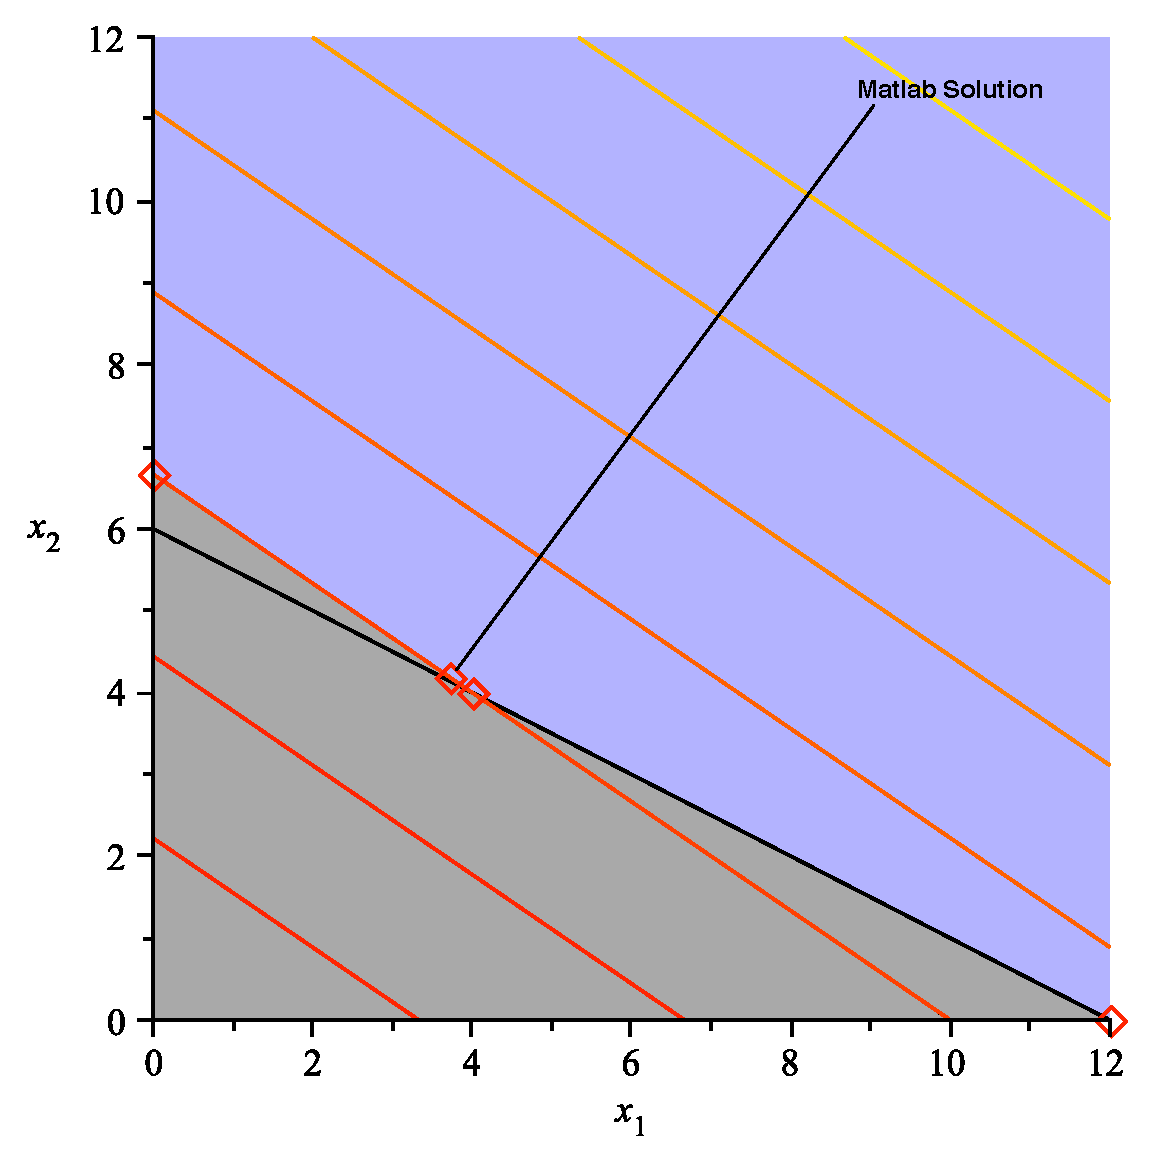
\includegraphics[scale=0.35]{DietProblemFigure.pdf}
\caption{The feasible region for the diet problem is unbounded and there are alternative optimal solutions, since we are seeking a minimum, we travel in the opposite direction of the gradient, so toward the origin to reduce the objective function value. Notice that the level curves hit one side of the boundary of the feasible region.}
\label{fig:DietProblem}
\end{figure}
If we continued in this way, we could actually construct all the points of intersection that make up the boundary of the feasible region. We'll can do one more, suppose $\mathbf{x}_\mathbf{B} = [x_1\;\;s_1]^T$. Then we would use Gauss-Jordan elimination to obtain:
\begin{displaymath}\left[
\begin{array}{cccc|c}
1 & 2 & 0 & -1 & 12\\
0 & 1 & 1 & -2 & 4
\end{array}\right]
\end{displaymath}
Notice there are now columns of the identity matrix in the columns corresponding to $s_1$ and $x_1$. That's how we know we're solving for $s_1$ and $x_2$. We have $x_1 = 12$ and $s_1 = 4$. By definition $x_1 = s_2 = 0$. This corresponds to the point $x_1 = 12, x_2 = 0$ shown in Figure \ref{fig:DietProblem}.

Let's use Matlab to solve this problem. Our original problem is:
\begin{displaymath}
\left\{
\begin{aligned}
\min\;\;& x_1 + 1.5x_2\\
s.t. \;\;& 2x_1 + 3x_2 \geq 20\\
& x_1 + 2x_2 \geq 12\\
&x_1, x_2 \geq 0
\end{aligned}\right.
\end{displaymath}

This is not in a form Matlab likes, so we change it by multiplying the constraints by $-1$ on both sides to obtain:
\begin{displaymath}
\left\{
\begin{aligned}
\min\;\;& x_1 + 1.5x_2\\
s.t. \;\;& -2x_1 - 3x_2 \leq -20\\
& -x_1 - 2x_2 \leq -12\\
&x_1, x_2 \geq 0
\end{aligned}\right.
\end{displaymath}

Then we have:
\begin{gather*}
\mathbf{c} = \begin{bmatrix}1\\1.5\end{bmatrix}\\
\mathbf{A} = \begin{bmatrix}-2 & -3\\-1 & -2\end{bmatrix}\\
\mathbf{b} = \begin{bmatrix}-20\\-12\end{bmatrix}\\
\mathbf{H} = \mathbf{r} = []\\
\mathbf{l} = \begin{bmatrix}0\\0\end{bmatrix}
\mathbf{u} = []
\end{gather*}
The Matlab code to solve this problem is shown in Figure \ref{fig:MatlabDiet}
\begin{figure}[htbp]
\centering
\scriptsize
\verbatiminput{SolveDietProblem.m}
\normalsize
\caption{Matlab input for solving the diet problem. Note that we are solving a \textit{minimization} problem. Matlab assumes all problems are \textit{mnimization} problems, so we don't need to multiply the objective by $-1$ like we would if we started with a maximization problem.}
\label{fig:MatlabDiet}
\end{figure}
The solution Matlab returns in the \texttt{x} variable is $x_1 = 3.7184$ and $x_2 = 4.1877$, note this is on the line of alternative optimal solutions, but it is not at either end of the line. I prefer to have a little less ice cream, so I'd rather have the alternative optimal solution $x_1 = x_2 = 4$.
\label{ex:Diet}
\end{example}

\begin{exercise} In previous example, you could also have just used the problem in standard form with the surplus variables and had $\mathbf{A} = \mathbf{b} = []$ and defined $\mathbf{H}$ and $\mathbf{r}$ instead. Use Matlab to solve the diet problem in \textit{standard form}. Compare your results to Example \ref{ex:Diet}
\end{exercise}
\chapter{Convex Sets, Functions and Cones and Polyhedral Theory}
In this chapter, we will cover all of the geometric prerequisites for understanding the theory of linear programming. We will use the results in this section to prove theorems about the Simplex Method in other sections.

\section{Convex Sets}
\begin{definition}[Convex Set] Let $X \subseteq \mathbb{R}^n$. Then the set $X$ is convex if and only if for all pairs $\mathbf{x}_1,\mathbf{x}_2 \in X$ we have $\lambda\mathbf{x}_1 + (1-\lambda)\mathbf{x}_2 \in X$ for all $\lambda \in [0,1]$.
\end{definition}

The definition of convexity seems complex, but it is easy to understand. First recall that if $\lambda \in [0,1]$, then the point $\lambda\mathbf{x}_1 + (1-\lambda)\mathbf{x}_2$ is on the line segment connecting $\mathbf{x}_1$ and $\mathbf{x}_2$ in $\mathbb{R}^n$. For example, when $\lambda = 1/2$, then the point $\lambda\mathbf{x}_1 + (1-\lambda)\mathbf{x}_2$ is the midpoint between $\mathbf{x}_1$ and $\mathbf{x}_2$. In fact, for every point $\mathbf{x}$ on the line connecting $\mathbf{x}_1$ and $\mathbf{x}_2$ we can find a value $\lambda \in [0,1]$ so that $\mathbf{x} = \lambda\mathbf{x}_1 + (1-\lambda)\mathbf{x}_2$. Then we can see that, convexity asserts that if $\mathbf{x}_1,\mathbf{x}_2 \in X$, then every point on the line connecting $\mathbf{x}_1$ and $\mathbf{x}_2$ is also in the set $X$. 

\begin{definition}[Positive Combination] Let $\mathbf{x}_1,\dots,\mathbf{x}_m \in \mathbb{R}^n$. If $\lambda_1,\dots,\lambda_m > 0$ and 
then 
\begin{equation}
\mathbf{x} = \sum_{i=1}^m\lambda_i\mathbf{x}_i
\end{equation}
is called a \textit{positive combination} of $\mathbf{x}_1,\dots,\mathbf{x}_m$.
\end{definition}

\begin{definition}[Convex Combination] Let $\mathbf{x}_1,\dots,\mathbf{x}_m \in \mathbb{R}^n$. If $\lambda_1,\dots,\lambda_m \in [0,1]$ and 
\begin{displaymath}
\sum_{i=1}^m\lambda_i = 1
\end{displaymath} 
then 
\begin{equation}
\mathbf{x} = \sum_{i=1}^m\lambda_i\mathbf{x}_i
\label{eqn:ConvexCombination}
\end{equation}
is called a \textit{convex combination} of $\mathbf{x}_1,\dots,\mathbf{x}_m$. If $\lambda_i < 1$ for all $i=1,\dots,m$, then Equation \ref{eqn:ConvexCombination} is called a \textit{strict convex combination}.
\end{definition}

\begin{remark} If you recall the definition of linear combination, we can see that we move from the very general to the very specific as we go from linear combinations to positive combinations to convex combinations. A linear combination of points or vectors allowed us to choose any real values for the coefficients. A positive combination restricts us to positive values, while a convex combination asserts that those values must be non-negative and sum to 1.
\end{remark}

\begin{example}
Figure \ref{fig:ConvexSets} illustrates a convex and non-convex set.
\begin{figure}[htbp]
\centering
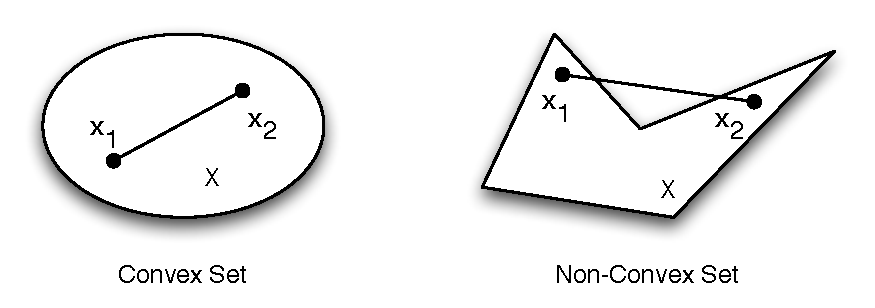
\includegraphics[scale=0.5]{ConvexSets.pdf}
\caption{Examples of Convex Sets: The set on the left (an ellipse and its interior) is a convex set; every pair of points inside the ellipse can be connected by a line contained entirely in the ellipse. The set on the right is clearly not convex as we've illustrated two points whose connecting line is not contained inside the set.}
\label{fig:ConvexSets}
\end{figure}
Non-convex sets have some resemblance to crescent shapes or have components that look like crescents.
\end{example}

\begin{theorem} The intersection of a finite number of convex sets in $\mathbb{R}^n$ is convex.
\end{theorem}
\begin{proof} Let $C_1,\dots,C_n \subseteq \mathbb{R}^n$  be a finite collection of convex sets. Let 
\begin{equation}
C = \bigcap_{i=1}^{n} C_i
\end{equation}
be the set formed from the intersection of these sets. Choose $\mathbf{x}_1,\mathbf{x}_2 \in C$ and $\lambda \in [0,1]$. Consider $\mathbf{x} = \lambda\mathbf{x}_1 + (1-\lambda)\mathbf{x}_2$. We know that $\mathbf{x}_1,\mathbf{x}_2 \in C_1,\dots,C_n$ by definition of $C$. By convexity, we know that $\mathbf{x} \in C_1,\dots,C_n$ by convexity of each set. Therefore, $\mathbf{x} \in C$. Thus $C$ is a convex set.
\end{proof}

\section{Convex and Concave Functions}
\begin{definition}[Convex Function] A function $f:\mathbb{R}^n \rightarrow \mathbb{R}$ is a convex function if it satisfies:
\begin{equation}
f(\lambda\mathbf{x}_1 + (1-\lambda)\mathbf{x}_2) \leq \lambda f(\mathbf{x}_1) + (1-\lambda)f(\mathbf{x}_2)
\end{equation}
for all $\mathbf{x}_1,\mathbf{x}_2 \in \mathbb{R}^n$ and for all $\lambda \in [0,1]$. 
\end{definition}
This definition is illustrated in Figure \ref{fig:QuadraticConvex}.
\begin{figure}[htbp]
\centering
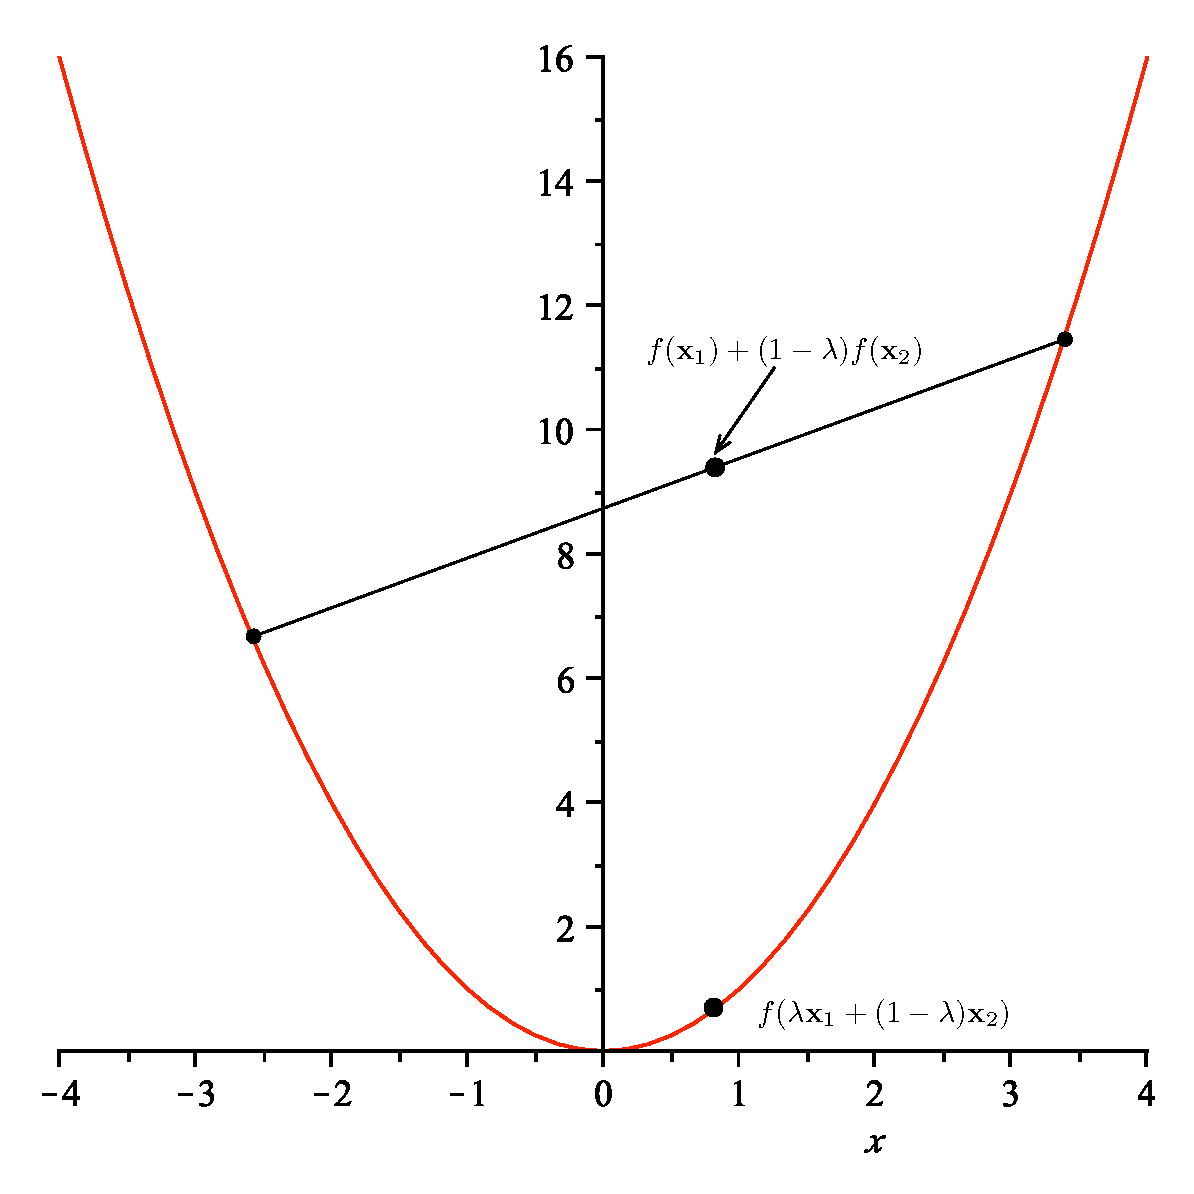
\includegraphics[scale=0.25]{QuadraticConvex.pdf}
\caption{A convex function: A convex function satisfies the expression $f(\lambda\mathbf{x}_1 + (1-\lambda)\mathbf{x}_2) \leq \lambda f(\mathbf{x}_1) + (1-\lambda)f(\mathbf{x}_2)$ for all $\mathbf{x}_1$ and $\mathbf{x}_2$ and $\lambda \in [0,1]$.}
\label{fig:QuadraticConvex}
\end{figure}
When $f$ is a univariate function, this definition can be shown to be equivalent to the definition you learned in Calculus I (Math 140) using first and second derivatives.
\begin{definition}[Concave Function] A function $f:\mathbb{R}^n \rightarrow \mathbb{R}$ is a concave function if it satisfies:
\begin{equation}
f(\lambda\mathbf{x}_1 + (1-\lambda)\mathbf{x}_2) \geq \lambda f(\mathbf{x}_1) + (1-\lambda)f(\mathbf{x}_2)
\end{equation}
for all $\mathbf{x}_1,\mathbf{x}_2 \in \mathbb{R}^n$ and for all $\lambda \in [0,1]$ \footnote{Thanks to Greg Ference and Veselka Kafedzhieva for catching a typo in this definition.}. 
\end{definition}
To visualize this definition, simply flip Figure \ref{fig:QuadraticConvex} upside down. The following theorem is a powerful tool that can be used to show sets are convex. It's proof is outside the scope of the class, but relatively easy. 
\begin{theorem} Let $f:\mathbb{R}^n \rightarrow \mathbb{R}$ be a convex function. Then the set $C = \{\mathbf{x} \in \mathbb{R}^n : f(x) \leq c\}$, where $c \in \mathbb{R}$, is a convex set. 
\label{thm:ConvexFunctionSet}
\end{theorem}

\begin{exercise} Prove the Theorem \ref{thm:ConvexFunctionSet}. [Hint: Skip ahead and read the proof of Lemma \ref{lem:HalfSpaceConvex}. Follow the steps in that proof, but apply them to $f$.]
\end{exercise}

\section{Polyhedral Sets}
Important examples of convex sets are polyhedral sets, the multi-dimensional analogs of polygons in the plane. In order to understand these structures, we must first understand hyperplanes and half-spaces. 

\begin{definition}[Hyperplane] Let $\mathbf{a} \in \mathbb{R}^n$ be a constant vector in $n$-dimensional space and let $b \in \mathbb{R}$ be a constant scalar. The set of points 
\begin{equation}
H = \left\{\mathbf{x} \in \mathbb{R}^n | 
\mathbf{a}^T\mathbf{x} = b\right\}
\end{equation}
is a \textit{hyperplane} in $n$-dimensional space. \textit{Note the use of column vectors for $\mathbf{a}$ and $\mathbf{x}$ in this definition.}
\end{definition}

\begin{example} Consider the hyper-plane $2x_1 + 3x_2 + x_3 = 5$. This is shown in Figure \ref{fig:HyperPlane}.
\begin{figure}[htbp]
\centering
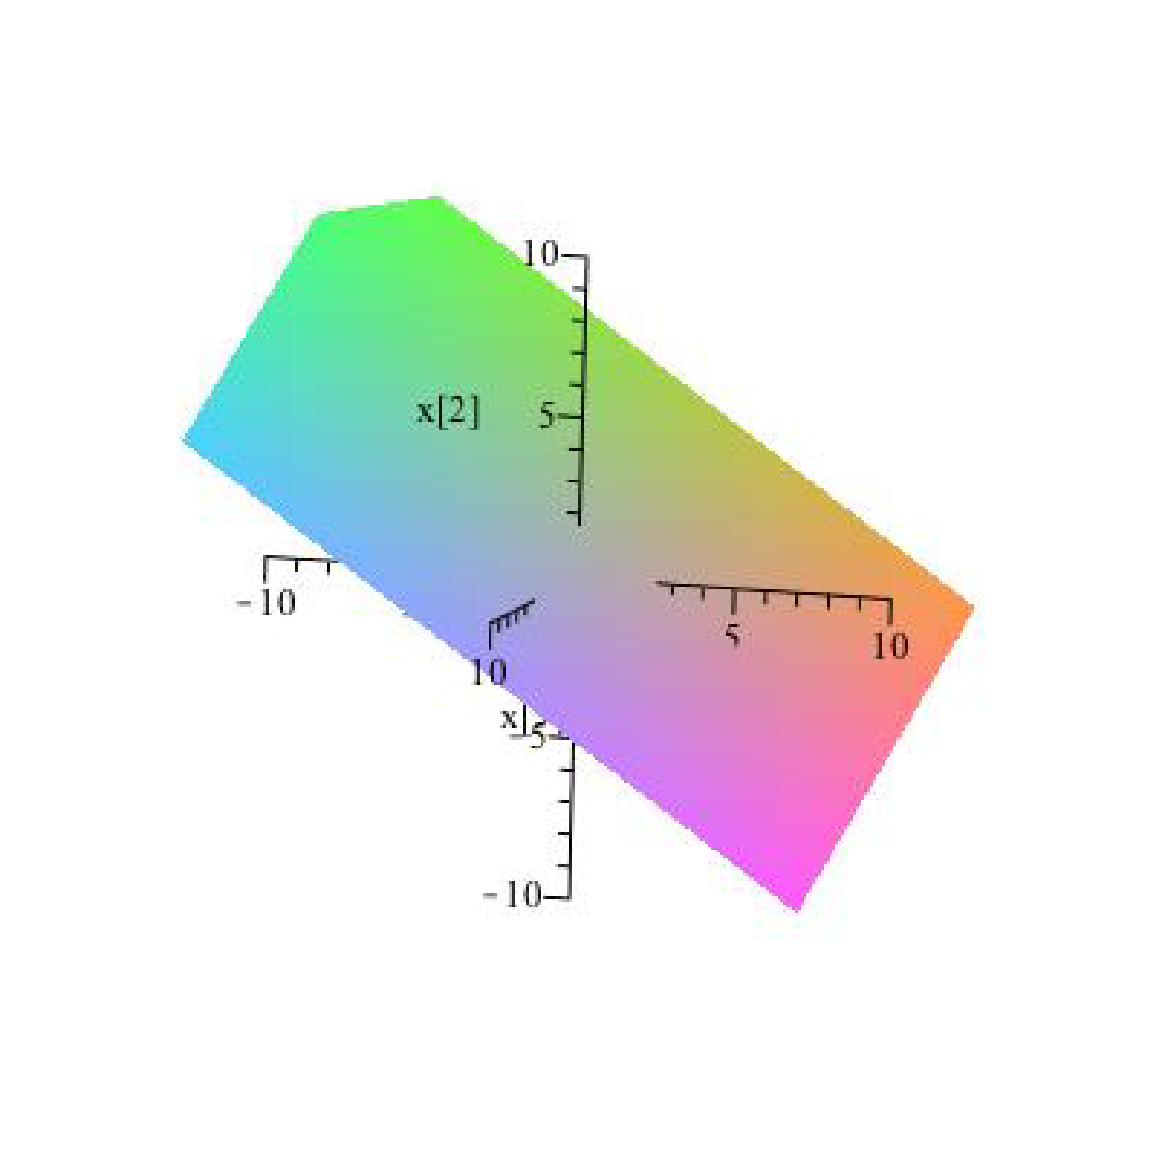
\includegraphics[scale=0.5]{HyperPlane.pdf}
\caption{A hyperplane in 3 dimensional space: A hyperplane is the set of points satisfying an equation $\mathbf{a}^T\mathbf{x} = b$, where $k$ is a constant in $\mathbb{R}$ and $\mathbf{a}$ is a constant vector in $\mathbb{R}^n$ and $\mathbf{x}$ is a variable vector in $\mathbb{R}^n$. The equation is written as a matrix multiplication using our assumption that all vectors are column vectors.}
\label{fig:HyperPlane}
\end{figure}
This hyperplane is composed of the set of points $(x_1,x_2,x_3) \in \mathbb{R}^3$ satisfying $2x_1 + 3x_2 + x_3 = 5$. This can be plotted implicitly or explicitly by solving for one of the variables, say $x_3$. We can write $x_3$ as a function of the other two variables as: 
\begin{equation}
x_3 = 5 - 2x_1 - 3x_2
\end{equation}
\end{example}

\begin{definition}[Half-Space] Let $\mathbf{a} \in \mathbb{R}^n$ be a constant vector in $n$-dimensional space and let $b \in \mathbb{R}$ be a constant scalar. The sets of points 
\begin{gather}
H_l = \left\{\mathbf{x} \in \mathbb{R}^n | \mathbf{a}^T\mathbf{x} \leq b\right\}\\
H_u = \left\{\mathbf{x} \in \mathbb{R}^n | \mathbf{a}^T\mathbf{x} \geq b\right\}
\end{gather} 
are the half-spaces defined by the hyperplane $\mathbf{a}^T\mathbf{x} = b$. 
\end{definition}
\begin{example} Consider the two dimensional hyperplane (line) $x_1 + x_2 = 1$. Then the two half-spaces associated with this hyper-plane are shown in Figure \ref{fig:HalfSpace}.
\begin{figure}[htbp]
\subfigure[$H_l$]{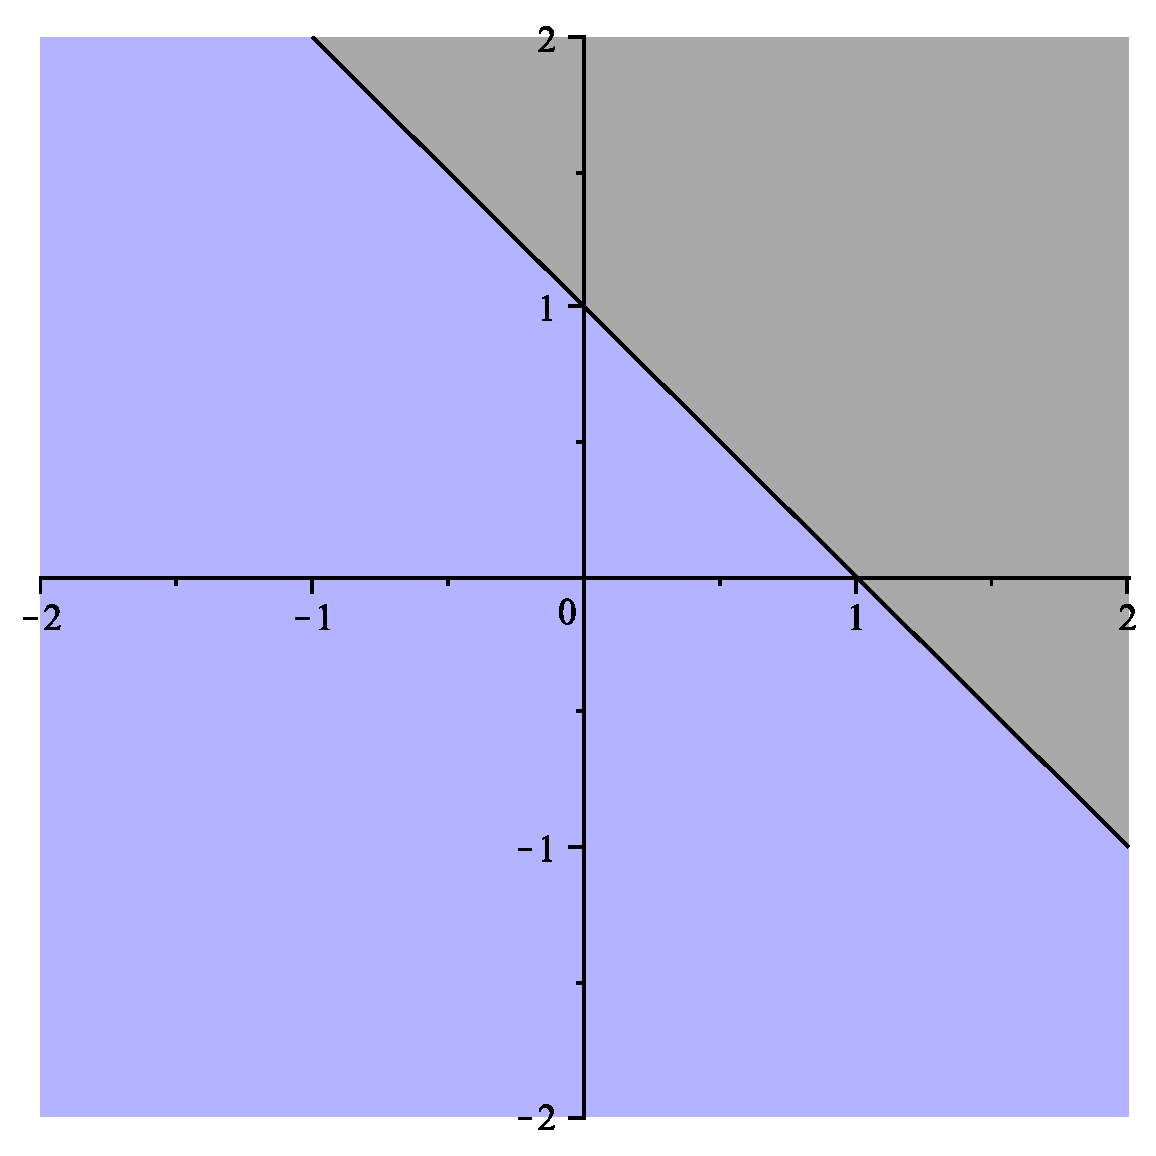
\includegraphics[scale=0.25]{Hl.pdf}}
\subfigure[$H_u$]{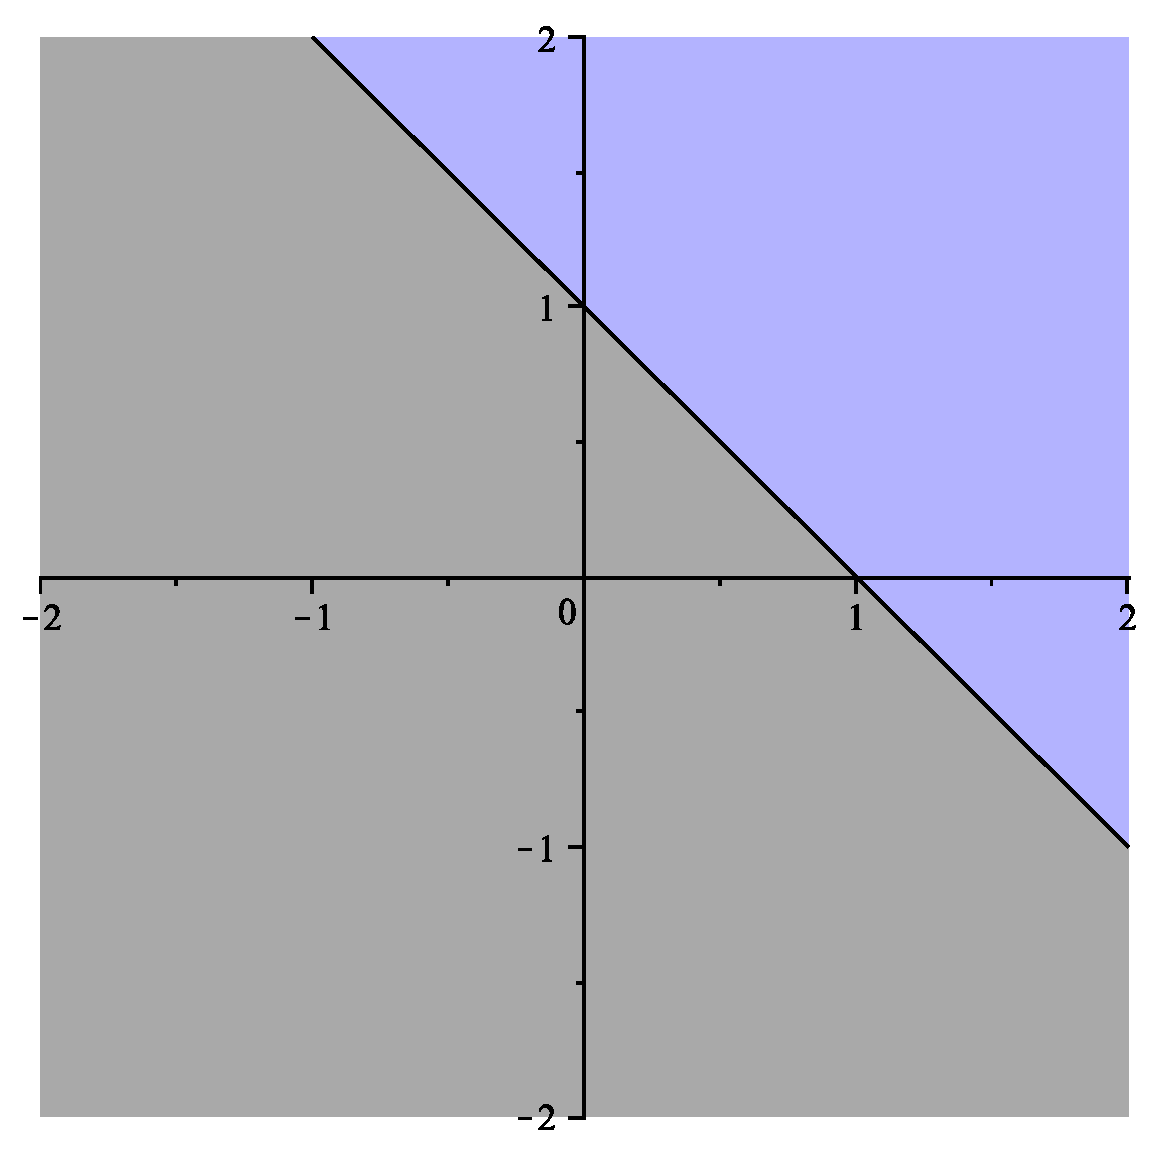
\includegraphics[scale=0.25]{Hu.pdf}}
\caption{Two half-spaces defined by a hyper-plane: A half-space is so named because any hyper-plane divides $\mathbb{R}^n$ (the space in which it resides) into two halves, the side ``on top'' and the side ``on the bottom.''}
\label{fig:HalfSpace}
\end{figure}
A half-space is so named because the hyperplane $\mathbf{a}^T\mathbf{x} = b$ literally separates $\mathbb{R}^n$ into two halves: the half above the hyperplane and the half below the hyperplane.
\end{example}

\begin{lemma} Every hyper-plane is convex.
\end{lemma}
\begin{proof} Let $\mathbf{a} \in \mathbb{R}^n$ and $b \in \mathbb{R}$ and let $H$ be the hyperplane defined by $\mathbf{a}$ and $b$. Choose $\mathbf{x}_1,\mathbf{x}_2 \in{H}$ and $\lambda \in [0,1]$. Let $\mathbf{x} = \lambda\mathbf{x}_1 + (1-\lambda)\mathbf{x}_2$.
By definition we know that:
\begin{gather*}
\mathbf{a}^T\mathbf{x}_1 = b\\
\mathbf{a}^T\mathbf{x}_2 = b
\end{gather*}
Then we have:
\begin{equation}
\mathbf{a}^T\mathbf{x} = \mathbf{a}^T\left[\lambda\mathbf{x}_1 + (1-\lambda)\mathbf{x}_2\right] = 
\lambda\mathbf{a}^T\mathbf{x}_1 + (1-\lambda)\mathbf{a}^T\mathbf{x}_2 = 
\lambda b + (1-\lambda)b = b
\end{equation}
Thus, $\mathbf{x} \in H$ and we see that $H$ is convex. This completes the proof.
\end{proof}
\begin{lemma} Every half-space is convex.
\label{lem:HalfSpaceConvex}
\end{lemma}
\begin{proof}
Let $\mathbf{a} \in \mathbb{R}^n$ and $b \in \mathbb{R}$. Without loss of generality, consider the half-space $H_l$ defined by $\mathbf{a}$ and $b$. For arbitrary $\mathbf{x}_1$ and $\mathbf{x}_2$ in $H_l$ we have:
\begin{gather*}
\mathbf{a}^T\mathbf{x}_1 \leq b\\
\mathbf{a}^T\mathbf{x}_2 \leq b
\end{gather*}
Suppose that $\mathbf{a}^T\mathbf{x}_1 = b_1 \leq b$ and $\mathbf{a}^T\mathbf{x}_2 = b_2 \leq b$. Again let $\mathbf{x} = \lambda\mathbf{x}_1 + (1-\lambda)\mathbf{x}_2$. Then:
\begin{equation}
\mathbf{a}^T\mathbf{x} = \mathbf{a}^T\left[\lambda\mathbf{x}_1 + (1-\lambda)\mathbf{x}_2\right] = 
\lambda\mathbf{a}^T\mathbf{x}_1 + (1-\lambda)\mathbf{a}^T\mathbf{x}_2 = 
\lambda b_1 + (1-\lambda)b_2
\end{equation}
Since $\lambda \leq 1$ and $1-\lambda \leq 1$ and $\lambda \geq 0$ we know that $\lambda b_1 \leq \lambda b$, since $b_1 \leq b$. Similarly we know that $(1-\lambda) b_2 \leq (1-\lambda)b$, since $b_2 \leq b$. Thus:
\begin{equation}
\lambda b_1 + (1-\lambda)b_2 \leq \lambda b + (1-\lambda)b=b
\end{equation}
Thus we have shown that $\mathbf{a}^T\mathbf{x} \leq b$. The case for $H_u$ is identical with the signs of the inequalities reversed. This completes the proof.
\end{proof}

Using these definitions, we are now in a position to define polyhedral sets, which will be the subject of our study for most of the remainder of this chapter. 

\begin{definition}[Polyhedral Set] If $P \subseteq \mathbb{R}^n$ is the intersection of a finite number of half-spaces, then $P$ is a \textit{polyhedral set}. Formally, let $\mathbf{a}_1,\dots,\mathbf{a}_m \in \mathbb{R}^n$ be a finite set of constant vectors and let $b_1,\dots,b_m \in \mathbb{R}$ be constants. Consider the set of half-spaces:
\begin{displaymath}
H_i = \{\mathbf{x} | \mathbf{a}_i^T\mathbf{x} \leq b_i\}
\end{displaymath}
Then the set:
\begin{equation}
P = \bigcap_{i=1}^m H_i
\end{equation}
is a \textit{polyhedral set}.
\label{defn:PolyhedralSet}
\end{definition}

It should be clear that we can represent any polyhedral set using a matrix inequality. The set $P$ is defined by the set of vectors $\mathbf{x}$ satisfying:
\begin{equation}
\mathbf{A}\mathbf{x} \leq \mathbf{b},
\end{equation}
where the \textit{rows} of $\mathbf{A} \in \mathbb{R}^{m \times n}$ are made up of the vectors $\mathbf{a}_1,\dots,\mathbf{a}_m$ and $\mathbf{b} \in \mathbb{R}^m$ is a column vector composed of elements $b_1,\dots,b_m$. 

\begin{theorem} Every polyhedral set is convex.
\label{thm:PolyhedralConvex}
\end{theorem}
\begin{exercise} Prove Theorem \ref{thm:PolyhedralConvex}. [Hint: You can prove this by brute force, verifying convexity. You can also be clever and use two results that we've proved in the notes.]
\end{exercise}

\section{Rays and Directions}
Recall the definition of a \textit{line} (Definition \ref{def:Line} from Chapter 1. A ray is a one sided line. 

\begin{definition}[Ray] Let $\mathbf{x}_0 \in \mathbb{R}^n$ be a point and and let $\mathbf{d} \in \mathbb{R}^n$ be a vector called the \textit{direction}. Then the \textit{ray} with vertex $\mathbf{x}_0$ and direction $\mathbf{d}$ is the collection of points $\{\mathbf{x} | \mathbf{x} = \mathbf{x}_0 + \lambda \mathbf{d},\;\lambda \geq 0\}$.
\end{definition}

\begin{example} We will use the same point and direction as we did for a line in Chapter 1. Let $\mathbf{x_0} = [2,1]^T$ and let $\mathbf{d} = [2,2]^T$. Then the ray defined by $\mathbf{x}_0$ and $\mathbf{d}$ is shown in Figure \ref{fig:LineExample}. The set of points is $R = \{(x,y) \in \mathbb{R}^2 : x = 2 + 2\lambda, y = 1 + 2\lambda, \lambda \geq 0\}$. 
\begin{figure}[ht]
\centering
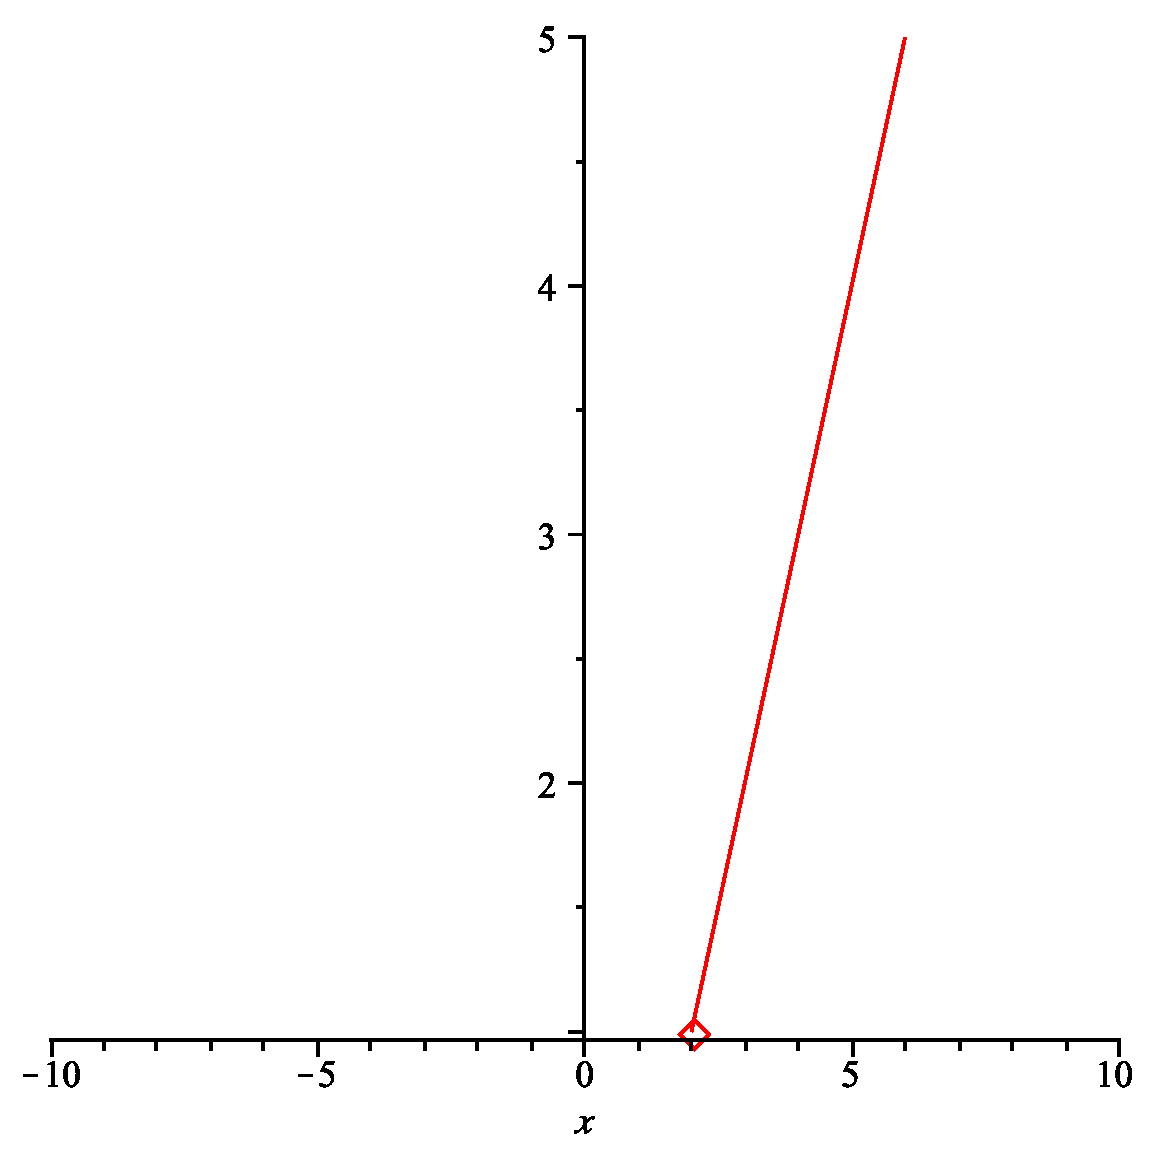
\includegraphics[scale=0.25]{Ray.pdf}
\caption{A Ray: The points in the graph shown in this figure are in the set produced using the expression $\mathbf{x}_0 + \mathbf{d}\lambda$ where $\mathbf{x_0} = [2,1]^T$ and $\mathbf{d} = [2,2]^T$ and $\lambda \geq 0$.}
\label{fig:RayExample}
\end{figure}
\label{ex:BasicRay}
\end{example}

Rays are critical for understanding unbounded convex sets. Specifically, a set is unbounded, in a sense, only if you can show that it contains a ray. An interesting class of unbounded convex sets are convex cones:

\begin{definition}[Convex Cone] Let $C \subseteq \mathbb{R}^n$ be a convex set. Then $C$ is a \textit{convex cone} if for all $\mathbf{x} \in C$ and for all $\lambda \in \mathbb{R}$ with $\lambda \geq 0$ we have $\lambda \mathbf{x} \in C$.
\end{definition}

\begin{lemma} Every convex cone contains the origin.
\label{lem:ConvexConeOrigin}
\end{lemma}

\begin{exercise} Prove the previous lemma. 
\end{exercise}

The fact that every convex cone contains the origin by Lemma \ref{lem:ConvexConeOrigin} along with the fact that for every point $\mathbf{x} \in C$ we have $\lambda\mathbf{x} \in C$ ($\lambda \geq 0$) implies that the ray $\mathbf{0} + \lambda\mathbf{x} \subseteq C$. Thus, since every point $\mathbf{x} \in C$ must be on a ray, it follows that a convex cone is just made up of rays beginning at the origin. 

Another key element to understanding unbounded convex sets is the notion of direction. A direction can be thought of as  a ``direction of travel'' from a starting point inside an unbounded convex set so that you (the traveler) can continue moving forever and never leave the set.

\begin{definition}[Direction of a Convex Set] Let $C$ be a convex set. Then $\mathbf{d}\neq \mathbf{0}$ is a \textit{(recession) direction of the convex set} if for all $\mathbf{x}_0 \in {C}$ the ray with vertex $\mathbf{x}_0$ and direction $\mathbf{d}$ is contained entirely in $C$. Formally, for all $\mathbf{x}_0 \in C$ we have:
\begin{equation}
\left\{\mathbf{x} : \mathbf{x} = \mathbf{x}_0 + \lambda\mathbf{d},\;\lambda \geq 0\right\} \subseteq C
\end{equation}
\end{definition}
\begin{example} Consider the unbounded convex set shown in Figure \ref{fig:ConvexDirectionExample}. This set has direction $[1,0]^T$. 
\begin{figure}[ht]
\centering
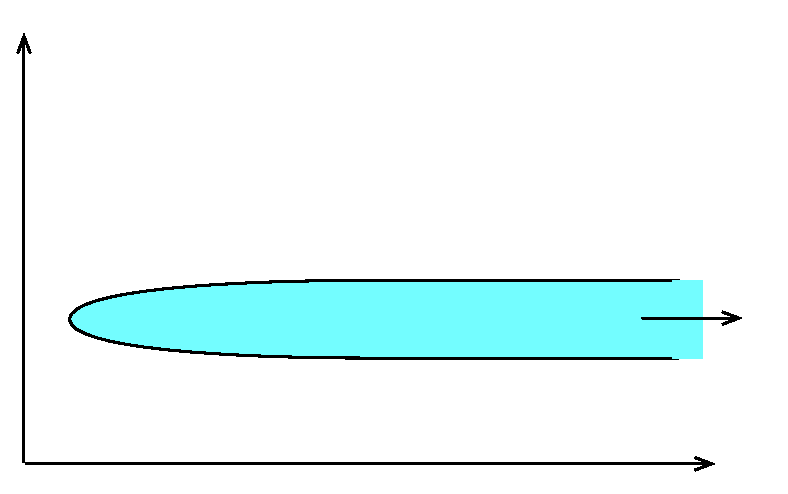
\includegraphics[scale=0.5]{ConvexDirection.pdf}
\caption{Convex Direction: Clearly every point in the convex set (shown in blue) can be the vertex for a ray with direction $[1,0]^T$ contained entirely in the convex set. Thus $[1,0]^T$ is a direction of this convex set.}
\label{fig:ConvexDirectionExample}
\end{figure}
To see this note that for any positive scaling parameter $\lambda$ and for any vertex point $\mathbf{x}_0$, we can draw an arrow pointing to the right (in the direction of $[1,0]^T$) with vertex at $\mathbf{x}_0$ scaled by $\lambda$ that is entirely contained in the convex set.
\end{example}

\begin{exercise} Prove the following: Let $C \subseteq \mathbb{R}^n$ be a convex cone and let $\mathbf{x}_1,\mathbf{x}_2 \in C$. If $\alpha, \beta \in \mathbb{R}$ and $\alpha,\beta \geq 0$, then $\alpha\mathbf{x}_1 + \beta\mathbf{x}_2 \in C$. [Hint: Use the definition of convex cone and the definition of convexity with $\lambda = 1/2$, then multiply by 2.] 
\label{exer:ConvexCone1}
\end{exercise}

\begin{exercise} Use Exercise \ref{exer:ConvexCone1} to prove that if $C \subseteq \mathbb{R}^n$ is a convex cone, then every element $\mathbf{x} \in C$ (except the origin) is also a direction of $C$.
\end{exercise}

\section{Directions of Polyhedral Sets}
There is a unique relationship between the defining matrix $\mathbf{A}$ of a polyhedral set $P$ and a direction of this set that is particularly useful when we assume that $P$ is located in the positive orthant of $\mathbb{R}^n$ (i.e., $\mathbf{x} \geq 0$ are defining constraints of $P$). 
\begin{theorem} Suppose that $P \subseteq \mathbb{R}^n$ is a polyhedral set defined by:
\begin{equation}
P = \left\{\mathbf{x} \in \mathbb{R}^n : \mathbf{A} \mathbf{x} \leq \mathbf{b},\;\mathbf{x} \geq \mathbf{0}\right\}
\end{equation}
If $\mathbf{d}$ is a direction of $P$, then the following hold:
\begin{equation}
\mathbf{A}\mathbf{d} \leq \mathbf{0},\:\mathbf{d} \geq \mathbf{0},\;\mathbf{d} \neq \mathbf{0}. 
\end{equation}
\label{thm:DirectionChar}
\end{theorem}
\begin{proof} The fact that $\mathbf{d} \neq \mathbf{0}$ is clear from the definition of direction of a convex set. Furthermore, $\mathbf{d}$ is a direction if and only if 
\begin{gather}
\mathbf{A}\left(\mathbf{x} + \lambda\mathbf{d}\right) \leq \mathbf{b}\\
\mathbf{x} + \lambda\mathbf{d} \geq \mathbf{0}
\end{gather}
for all $\lambda > 0$ and for all $\mathbf{x} \in P$ (which is to say $\mathbf{x}\in \mathbb{R}^n$ such that $\mathbf{A}\mathbf{x} \leq \mathbf{b}$ and $\mathbf{x} \geq \mathbf{0}$). But then 
\begin{displaymath}
\mathbf{A}\mathbf{x} + \lambda\mathbf{A}\mathbf{d} \leq \mathbf{b}
\end{displaymath}
for all $\lambda > 0$. This can only be true if $\mathbf{A}\mathbf{d} \leq \mathbf{0}$. Likewise:$\mathbf{x} + \lambda\mathbf{d} \geq \mathbf{0}$ holds for all $\lambda > 0$ if and only if $\mathbf{d} \geq \mathbf{0}$. This completes the proof.
\end{proof}
\begin{corollary} If 
\begin{equation}
P = \left\{\mathbf{x} \in \mathbb{R}^n : \mathbf{A} \mathbf{x} = \mathbf{b},\;\mathbf{x} \geq \mathbf{0}\right\}
\end{equation}
and $\mathbf{d}$ is a direction of $P$, then $\mathbf{d}$ must satisfy:
\begin{equation}
\mathbf{A}\mathbf{d} = \mathbf{0},\:\mathbf{d} \geq \mathbf{0},\;\mathbf{d} \neq \mathbf{0}. 
\end{equation}
\end{corollary}
\begin{exercise} Prove the corollary above.
\end{exercise}

\begin{example} Consider the polyhedral set defined by the equations:
\begin{gather*}
x_1 - x_2 \leq 1\\
2x_1 + x_2 \geq 6\\
x_1 \geq 0\\
x_2 \geq 0
\end{gather*}
This set is clearly unbounded as we showed in class and it has at least one direction. The direction $\mathbf{d} = [0,1]^T$ pointing directly up is a direction of this set. This is illustrated in Figure \ref{fig:UnboundedPolyhedron}.
\begin{figure}[htbp]
\centering
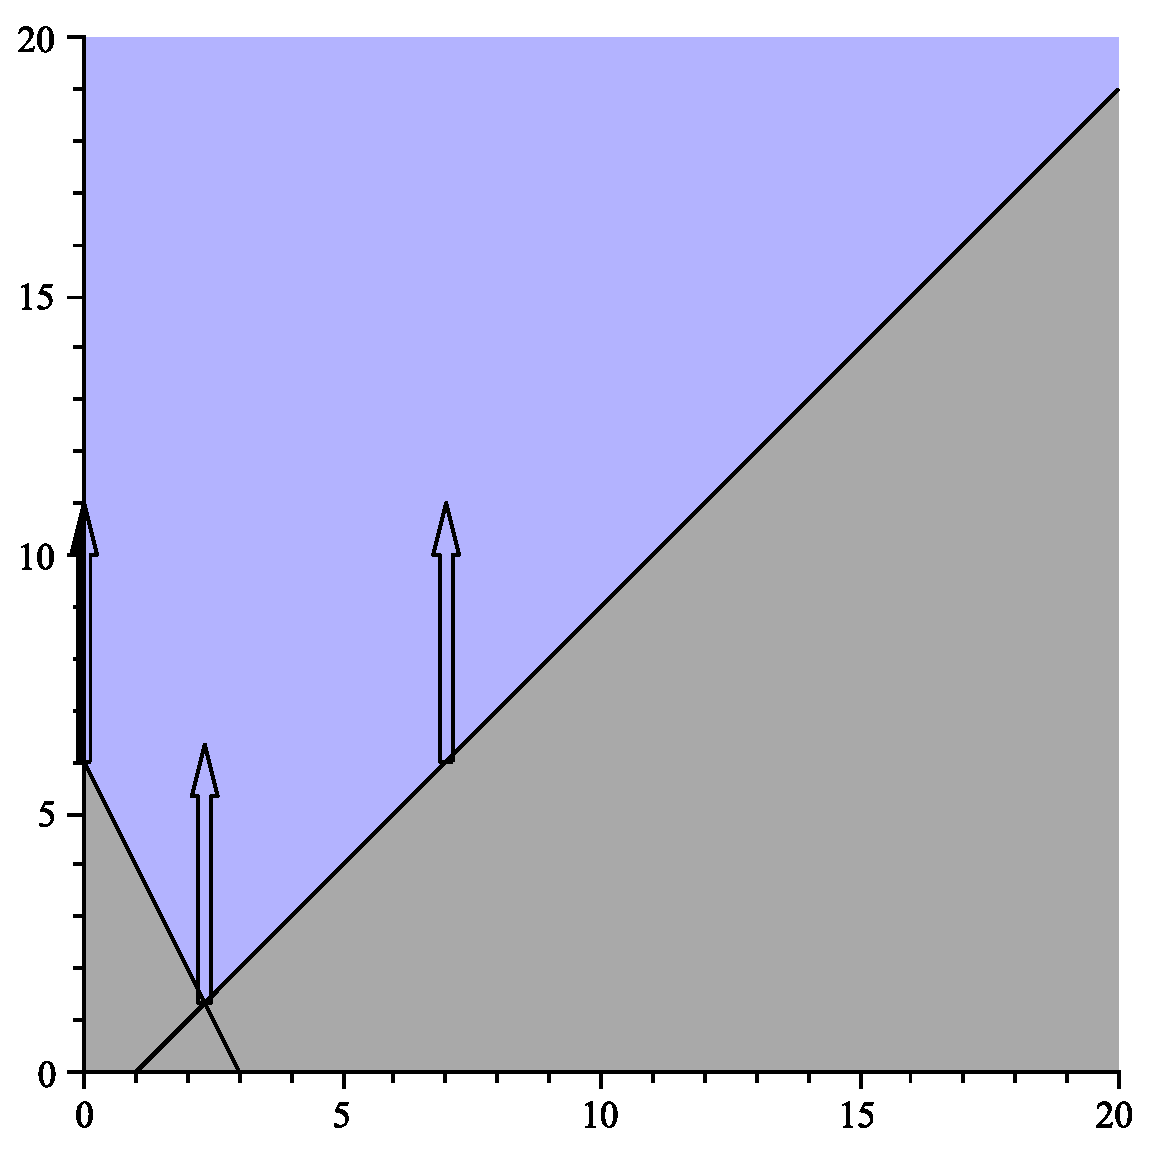
\includegraphics[scale=0.35]{UnboundedPolyhedron.pdf}
\caption{An Unbounded Polyhedral Set: This unbounded polyhedral set has many directions. One direction is $[0,1]^T$.}
\label{fig:UnboundedPolyhedron}
\end{figure}
In this example, we have:
\begin{equation}
\mathbf{A} = \begin{bmatrix}
1 & -1\\
-2 & -1
\end{bmatrix}
\end{equation}
Note, the second inequality constraint was a greater-than constraint. We reversed it to a less-than inequality constraint $-2x_1 - x_2 \leq -6$ by multiplying by $-1$. For our chosen direction $\mathbf{d} = [0,1]^T$, we can see that:
\begin{equation}
\mathbf{A}\mathbf{d} = 
\begin{bmatrix}
1 & -1\\
-2 & -1
\end{bmatrix}
\begin{bmatrix}
0\\
1
\end{bmatrix} = 
\begin{bmatrix}
-1\\
-1
\end{bmatrix} \leq \mathbf{0}
\end{equation}
Clearly $\mathbf{d} \geq \mathbf{0}$ and $\mathbf{d} \neq \mathbf{0}$.
\label{ex:UnboundedPolyhedron}
\end{example}

\section{Extreme Points}
\begin{definition}[Extreme Point of a Convex Set] Let $C$ be a convex set. A point $\mathbf{x}_0 \in C$ is a \textit{extreme point} of $C$ if there are \textit{no points} $\mathbf{x}_1$ and $\mathbf{x}_2$ ($\mathbf{x}_1 \neq \mathbf{x}_0$ or $\mathbf{x}_2 \neq \mathbf{x}_0$) so that
$\mathbf{x} = \lambda\mathbf{x}_1 + (1-\lambda)\mathbf{x}_2$ for some $\lambda \in (0,1)$.\footnote{Thanks to Bob Pakzad-Hurson who fixed a typo in this definition in Version $\leq$ 1.4.}
\label{defn:ExtremePoint}
\end{definition}

An extreme point is simply a point in a convex set $C$ that cannot be expressed as a strict convex combination of any other pair of points in $C$. We will see that extreme points must be located in specific locations in convex sets. 

\begin{definition}[Boundary of a set] Let $C \subseteq \mathbb{R}^n$ be (convex) set. A point $\mathbf{x}_0 \in C$ is on the \textit{boundary} of $C$ if for all $\epsilon > 0$, 
\begin{gather*}
B_\epsilon(\mathbf{x}_0) \cap C \neq \emptyset \;\text{and}\\
B_\epsilon(\mathbf{x}_0) \cap \mathbb{R}^n \setminus C \neq \emptyset
\end{gather*}
\end{definition}
\begin{example} A convex set, its boundary and a boundary point are illustrated in Figure \ref{fig:BoundaryPoint}.
\begin{figure}[htbp]
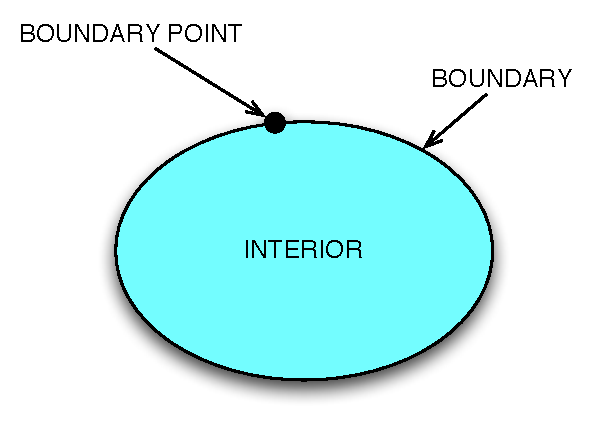
\includegraphics[scale=0.5]{Boundary.pdf}
\caption{Boundary Point: A boundary point of a (convex) set $C$ is a point in the set so that for \textit{every} ball of any radius centered at the point contains some points inside $C$ and some points outside $C$.}
\label{fig:BoundaryPoint}
\end{figure}
\end{example}

\begin{lemma} Suppose $C$ is a convex set. If $\mathbf{x}$ is an extreme point of $C$, then $\mathbf{x}$ is on the boundary of $C$. 
\label{lem:BoundaryExtremePoint}
\end{lemma}
\begin{proof} Suppose not, then $\mathbf{x}$ is not on the boundary and thus there is some $\epsilon > 0$ so that $B_\epsilon(\mathbf{x}_0) \subset C$. Since $B_\epsilon(\mathbf{x}_0)$ is a hypersphere, we can choose two points $\mathbf{x}_1$ and $\mathbf{x}_2$ on the boundary of $B_\epsilon(\mathbf{x}_0)$ so that the line segment between these points passes through the center of $B_\epsilon(\mathbf{x}_0)$. But this center point is $\mathbf{x}_0$. Therefore $\mathbf{x}_0$ is the mid-point of $\mathbf{x}_1$ and $\mathbf{x}_2$ and since $\mathbf{x}_1,\mathbf{x}_2 \in C$ and $\lambda\mathbf{x}_1 + (1-\lambda)\mathbf{x}_2 = \mathbf{x}_0$ with $\lambda = 1/2$ it follows that $\mathbf{x}_0$ cannot be an extreme point, since it is a strict convex combination of $\mathbf{x}_1$ and $\mathbf{x}_2$. This completes the proof.
\end{proof}

Most important in our discussion of linear programming will be the extreme points of polyhedral sets that appear in linear programming problems. The following theorem establishes the relationship between extreme points in a polyhedral set and the intersection of hyperplanes in such a set.

\begin{theorem} Let $P \subseteq \mathbb{R}^n$ be a polyhedral set and suppose $P$ is defined as:
\begin{equation}
P = \{\mathbf{x} \in \mathbb{R}^n : \mathbf{A}\mathbf{x} \leq \mathbf{b}\}
\end{equation}
where $\mathbf{A} \in \mathbb{R}^{m \times n}$ and $\mathbf{b} \in \mathbb{R}^m$. A point $\mathbf{x}_0 \in P$ is an extreme point of $P$ if and only if $\mathbf{x}_0$ is the intersection of $n$ linearly independent hyperplanes from the set defining $P$. 
\label{thm:DefExtremePoint}
\end{theorem}

\begin{remark}The easiest way to see this as relevant to linear programming is to assume that 
\begin{equation}
P = \{\mathbf{x} \in \mathbb{R}^n : \mathbf{A}\mathbf{x} \leq \mathbf{b},\;\mathbf{x} \geq \mathbf{0}\}
\end{equation}
In this case, we could have $m < n$. In that case, $P$ is composed of the intersection of $n + m$ half-spaces. The first $m$ are for the rows of $\mathbf{A}$ and the second $n$ are for the non-negativity constraints. An extreme point comes from the intersection of $n$ of the hyperplanes defining these half-spaces. We  might have $m$ come from the constraints $\mathbf{A}\mathbf{x} \leq \mathbf{b}$ and the other $n-m$ from $\mathbf{x} \geq \mathbf{0}$.
\end{remark}

\begin{proof}
($\Leftarrow$) Suppose that $\mathbf{x}_0$ is the intersection of $n$ hyperplanes. Then $\mathbf{x}_0$ lies on $n$ hyperplanes. By way of contradiction of suppose that $\mathbf{x}_0$ is not an extreme point. Then there are two points $\overline{\mathbf{x}}, \hat{\mathbf{x}} \in P$ and a scalar $\lambda \in (0,1)$ so that
\begin{displaymath}
\mathbf{x}_0 = \lambda\overline{\mathbf{x}} + (1-\lambda)\hat{\mathbf{x}}
\end{displaymath}
If this is true, then for some $\mathbf{G} \in \mathbb{R}^{n\times n}$ whose rows are drawn from $\mathbf{A}$ and a vector $\mathbf{g}$ whose entries are drawn from the vector $\mathbf{b}$, so that $\mathbf{G}\mathbf{x}_0 = \mathbf{g}$. But then we have:
\begin{equation}
\mathbf{g} = \mathbf{G}\mathbf{x}_0 = \lambda\mathbf{G}\overline{\mathbf{x}} + (1-\lambda)\mathbf{G}\hat{\mathbf{x}}
\label{eqn:gequal}
\end{equation}  
and $\mathbf{G}\overline{\mathbf{x}} \leq \mathbf{g}$ and $\mathbf{G}\hat{\mathbf{x}}\leq \mathbf{g}$ (since $\overline{\mathbf{x}}, \hat{\mathbf{x}} \in P$). But the only way for Equation \ref{eqn:gequal} to hold is if 
\begin{enumerate*}
\item $\mathbf{G}\overline{\mathbf{x}} = \mathbf{g}$ and
\item $\mathbf{G}\hat{\mathbf{x}} = \mathbf{g}$
\end{enumerate*}
The fact that the hyper-planes defining $\mathbf{x}_0$ are linearly independent implies that the solution to $\mathbf{G}\mathbf{x}_0 = \mathbf{g}$ is unique. (That is, we have chosen $n$ equations in $n$ unknowns and $\mathbf{x}_0$ is the solution to these $n$ equations.) Therefore, it follows that $\mathbf{x}_0 = \overline{\mathbf{x}}=\hat{\mathbf{x}}$ and thus $\mathbf{x}_0$ is an extreme point since it cannot be expressed as a convex combination of other points in $P$.

($\Rightarrow$) By Lemma \ref{lem:BoundaryExtremePoint}, we know that any extreme point $\mathbf{x}_0$ lies on the boundary of $P$ and therefore there is at least one row $\mathbf{A}_{i\cdot}$ such that $\mathbf{A}_{i\cdot}\mathbf{x}_0 = \mathbf{b}_i$ (otherwise, clearly $\mathbf{x}_0$ does not lie on the boundary of $P$). By way of contradiction, suppose that $\mathbf{x}_0$ is the intersection of $r < n$ linearly independent hyperplanes (that is, only these $r$ constraints are binding). Then there is a matrix $\mathbf{G} \in \mathbb{R}^{r \times n}$ whose rows are drawn from $\mathbf{A}$ and a vector $\mathbf{g}$ whose entries are drawn from the vector $\mathbf{b}$, so that $\mathbf{G}\mathbf{x}_0 = \mathbf{g}$. Linear independence of the hyperplanes implies that the rows of $\mathbf{G}$ are linearly independent and therefore there is a non-zero solution to the equation $\mathbf{G}\mathbf{d} = \mathbf{0}$. To see this, apply Expression \ref{eqn:BasicVars} and choose solution in which $\mathbf{d}$ is non-zero. Then we can find an $\epsilon > 0$ such that:
\begin{enumerate*}
\item If $\overline{\mathbf{x}} = \mathbf{x}_0 + \epsilon\mathbf{d}$, then $\mathbf{G}\overline{\mathbf{x}} = \mathbf{g}$ \textit{and} all non-binding constraints at $\mathbf{x}_0$ remain non-binding at $\overline{\mathbf{x}}$.

\item If $\hat{\mathbf{x}} = \mathbf{x}_0 - \epsilon\mathbf{d}$, then $\mathbf{G}\hat{\mathbf{x}} = \mathbf{g}$ \textit{and} all non-binding constraints at $\mathbf{x}_0$ remain non-binding at $\hat{\mathbf{x}}$.
\end{enumerate*}
These two facts hold since $\mathbf{G}\mathbf{d} = \mathbf{0}$ and if $\mathbf{A}_{i\cdot}$ is a row of $\mathbf{A}$ with $\mathbf{A}_{i\cdot}\mathbf{x}_0 < \mathbf{b}_i$ (or $\mathbf{x} > 0$), then there is at least one non-zero $\epsilon$ so that $\mathbf{A}_{i\cdot}(\mathbf{x}_0 \pm \epsilon \mathbf{d}) < \mathbf{b}_i$ (or $\mathbf{x}_0 \pm \epsilon \mathbf{d} > \mathbf{0}$) still holds and therefore $(\mathbf{x}_0 \pm \epsilon \mathbf{d}) \in P$. Since we have a finite number of constraints that are non-binding, we may choose $\epsilon$ to be the smallest value so that the previous statements hold for all of them. Finally we can choose $\lambda = 1/2$ and see that $\mathbf{x}_0 = \lambda\overline{\mathbf{x}} + (1-\lambda)\hat{\mathbf{x}}$ and $\overline{\mathbf{x}}, \hat{\mathbf{x}} \in P$. Thus $\mathbf{x}_0$ cannot have been an extreme point, contradicting our assumption. This completes the proof.
\end{proof}

\begin{definition} Let $P$ be the polyhedral set from Theorem \ref{thm:DefExtremePoint}. If $\mathbf{x}_0$ is an extreme point of $P$ and \textit{more} than $n$ hyperplanes are binding at $\mathbf{x}_0$, then $\mathbf{x}_0$ is called a \textit{degenerate} extreme point.
\end{definition}

\begin{definition}[Face] Let $P$ be a polyhedral set defined by
\begin{displaymath}
P = \{\mathbf{x} \in \mathbb{R}^n : \mathbf{A}\mathbf{x} \leq \mathbf{b}\}
\end{displaymath}
where $\mathbf{A} \in \mathbb{R}^{m\times n}$ and $\mathbf{b} \in \mathbb{R}^m$. If $X \subseteq P$ is defined by a non-empty set of binding linearly independent hyperplanes, then $X$ is a \textit{face} of $P$. 

That is, there is some set of linearly independent rows $A_{i_1\cdot},\dots A_{i_l\cdot}$ with $i_l < m$ so that when $\mathbf{G}$ is the matrix made of these rows and $\mathbf{g}$ is the vector of $b_{i_1},\dots,b_{i_l}$ then: 
\begin{equation}
X = \{\mathbf{x} \in \mathbb{R}^n : \mathbf{G}\mathbf{x} = \mathbf{g} \text{ and } \mathbf{A}\mathbf{x} \leq \mathbf{b}\}
\end{equation}
In this case we say that $X$ has \textit{dimension} $n - l$. 
\end{definition}

\begin{remark} Based on this definition, we can easily see that an extreme point, which is the intersection $n$ linearly independent hyperplanes is a face of dimension zero. 
\end{remark}

\begin{definition}[Edge and Adjacent Extreme Point] An edge of a polyhedral set $P$ is any face of dimension 1. Two extreme points are called \textit{adjacent} if they share $n-1$ binding constraints. That is, they are connected by an edge of $P$.
\end{definition} 

\begin{example} Consider the polyhedral set defined by the system of inequalities:
\begin{gather*}
3x_1 + x_2 \leq 120\\
x_1 + 2x_2 \leq 160\\
\frac{28}{16}x_1+x_2 \leq 100\\
x_1 \leq 35\\
x_1 \geq 0\\
x_2 \geq 0
\end{gather*}
The polyhedral set is shown in Figure \ref{fig:PolyhedralSet}.
\begin{figure}[htbp]
\centering
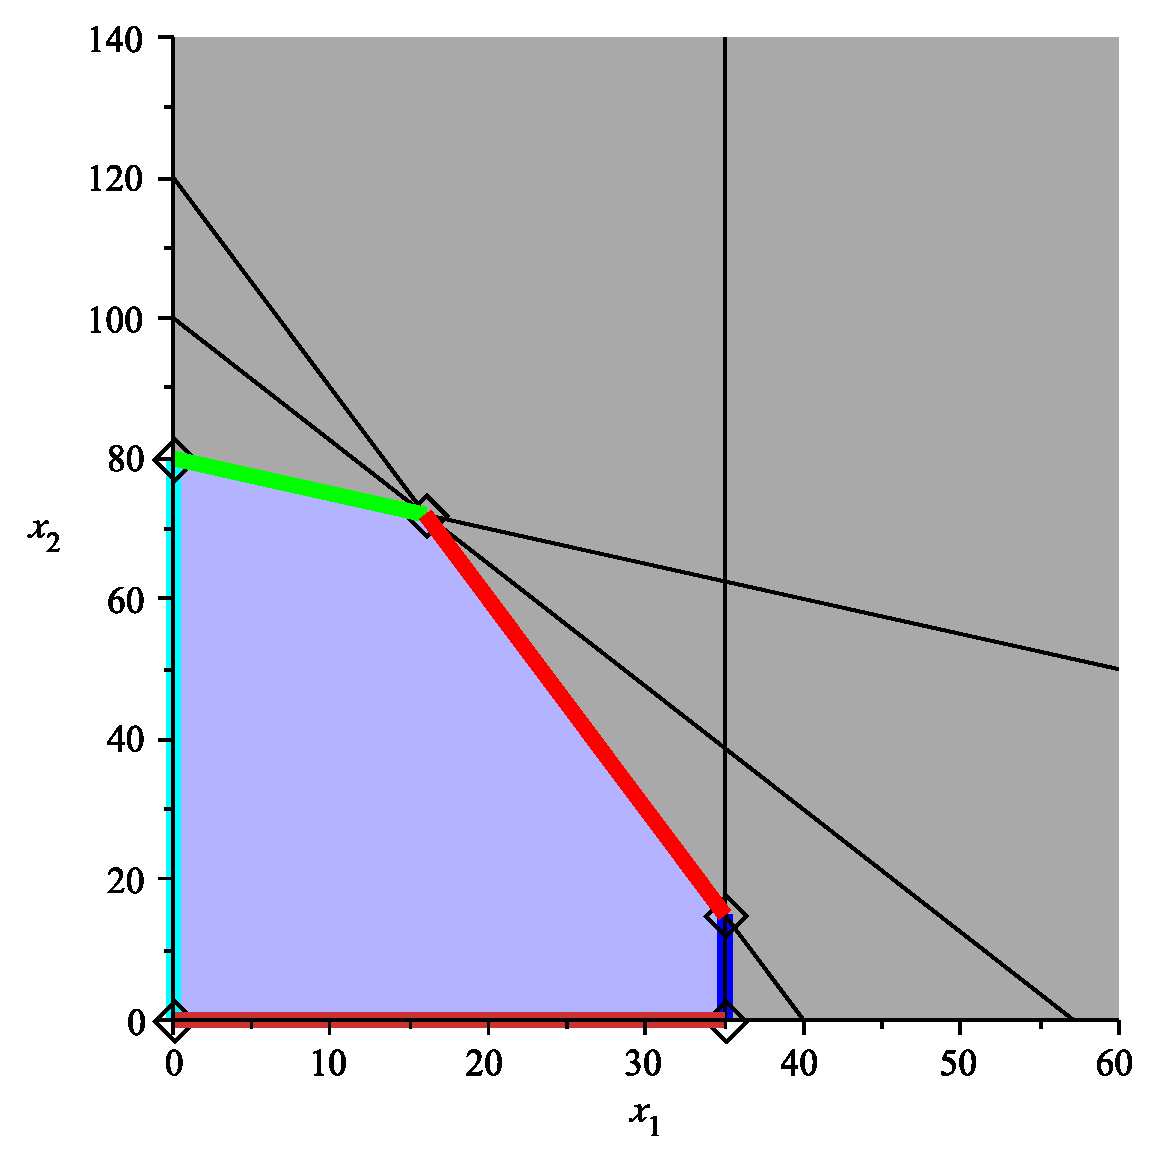
\includegraphics[scale=0.35]{PolyhedronExample.pdf}
\caption{A Polyhedral Set: This polyhedral set is defined by five half-spaces and has a single degenerate extreme point located at the intersection of the binding constraints $3x_1 + x_2 \leq 120$, $x_1 + 2x_2 \leq 160$ and $\frac{28}{16}x_1+x_2 <= 100$. All faces are shown in bold.}
\label{fig:PolyhedralSet}
\end{figure}
The extreme points of the polyhedral set are shown as large diamonds and correspond to intersections of binding constraints. Note the extreme point $(16,72)$ is \textit{degenerate} since it occurs at the intersection of three binding constraints $3x_1 + x_2 \leq 120$, $x_1 + 2x_2 \leq 160$ and $\frac{28}{16}x_1+x_2 <= 100$. All the faces of the polyhedral set are shown in bold. They are locations where one constraint (or half-space) is binding. An example of a pair of adjacent extreme points is $(16,72)$ and $(35,15)$, as they are connected by the edge defined by the binding constraint $3x_1 + x_2 \leq 120$.
\label{ex:ToyMakerDegen}
\end{example}

\begin{exercise} Consider the polyhedral set defined by the system of inequalities:
\begin{gather*}
4x_1 + x_2 \leq 120\\
x_1 + 8x_2 \leq 160\\
x_1 + x_2 \leq 30\\
x_1 \geq 0\\
x_2 \geq 0
\end{gather*}
Identify all extreme points and edges in this polyhedral set and their binding constraints. Are any extreme points degenerate? List all pairs of adjacent extreme points.
\end{exercise}

\section{Extreme Directions}
\begin{definition}[Extreme Direction] Let $C \subseteq\mathbb{R}^n$ be a convex set. Then a direction $\mathbf{d}$ of $C$ is an \textit{extreme direction} if there are no two other directions $\mathbf{d}_1$ and $\mathbf{d}_2$ of $C$ ($\mathbf{d}_1 \neq \mathbf{d}$ and $\mathbf{d}_2 \neq \mathbf{d}$) and scalars $\lambda_1,\lambda_2 > 0$ so that $\mathbf{d} = \lambda_1\mathbf{d}_1 + \lambda_2\mathbf{d}_2$. 
\end{definition}

We have already seen by Theorem \ref{thm:DirectionChar} that is $P$ is a polyhedral set in the positive orthant of $\mathbb{R}^n$ with form:
\begin{displaymath}
P = \left\{\mathbf{x} \in \mathbb{R}^n : \mathbf{A} \mathbf{x} \leq \mathbf{b},\;\mathbf{x} \geq \mathbf{0}\right\}
\end{displaymath}
then a direction $\mathbf{d}$ of $P$ is characterized by the set of inequalities and equations
\begin{displaymath}
\mathbf{A}\mathbf{d} \leq \mathbf{0},\:\mathbf{d} \geq \mathbf{0},\;\mathbf{d} \neq \mathbf{0}.
\end{displaymath}
Clearly two directions $\mathbf{d}_1$ and $\mathbf{d}_2$ with $\mathbf{d_1} = \lambda\mathbf{d}_2$ for some $\lambda \geq 0$ may both satisfy this system. To isolate a unique set of directions, we can normalize and construct the set:
\begin{equation}
D = \{\mathbf{d} \in \mathbb{R}^n : \mathbf{A}\mathbf{d} \leq \mathbf{0},\;\mathbf{d} \geq \mathbf{0},\mathbf{e}^T\mathbf{d} = 1\}
\end{equation}
here we are interested only in directions satisfying $\mathbf{e}^T\mathbf{d} = 1$. This is a normalizing constraint that will chose only vectors whose components sum to 1.

\begin{theorem} A direction $\mathbf{d} \in D$ is an extreme direction of $P$ if and only if $\mathbf{d}$ is an extreme point of $D$ when $D$ is taken as a polyhedral set.
\label{thm:ExtremeDirections}
\end{theorem}
\begin{proof} 
($\Rightarrow$)Suppose that $\mathbf{d}$ is an extreme point of $D$ (as a polyhedral set) and not an extreme direction of $P$. Then there exist two directions $\mathbf{d}_1$ and $\mathbf{d}_2$ of $P$ and two constants $\lambda_1$ and $\lambda_2$ with $\lambda_1,\lambda_2 \geq 0$ so that $\mathbf{d} = \lambda_1\mathbf{d}_1 + \lambda_2\mathbf{d}_2$. Without loss of generality, we may assume that $\mathbf{d}_1$ and $\mathbf{d}_2$ are vectors satisying $\mathbf{e}^T\mathbf{d}_i = 1$ ($i=1,2$). If not, then we can scale them so their components sum to 1 and adjust $\lambda_1$ and $\lambda_2$ accordingly. But this implies that:
\begin{displaymath}
1 = \mathbf{e}^T\mathbf{d} = \lambda_1 \mathbf{e}^T\mathbf{d}_1 + \lambda_2\mathbf{e}^T\mathbf{d}_2 = \lambda_1 + \lambda_2
\end{displaymath}
Further, the fact that $\mathbf{d}_1$ and $\mathbf{d}_2$ are directions of $P$ implies they must be in $D$. Thus we have found a convex combination of element of $D$ that equals $\mathbf{d}$, contradicting our assumption that $\mathbf{d}$ was an extreme point.

($\Leftarrow$)Conversely, suppose that $\mathbf{d}$ is an extreme direction  of $P$ whose components sum to 1 and not an extreme point of $D$. (Again, we could scale $\mathbf{d}$ if needed.) Then $\mathbf{d}$ cannot be recovered from a positive combination of directions $\mathbf{d}_1$ and $\mathbf{d}_2$. But if $\mathbf{d}$ is not an extreme point of $D$, then we know $\lambda_1\mathbf{d}_1 + \lambda_2\mathbf{d}_2 = \mathbf{d}$ for $\mathbf{d}_1,\mathbf{d}_2 \in D$ and $\lambda_1 + \lambda_2 = 1$ and $\lambda_1,\lambda_2 \in (0,1)$. This is clearly contradictory. Every strict convex combination is a positive combination and therefore our assumption that $\mathbf{d}$ was an extreme direction was false.
\end{proof}

\begin{example} Let's consider Example \ref{ex:UnboundedPolyhedron} again. The polyhedral set in this example was defined by the $\mathbf{A}$ matrix:
\begin{displaymath}
\mathbf{A} = \begin{bmatrix}
1 & -1\\
-2 & -1
\end{bmatrix}
\end{displaymath} 
and the $\mathbf{b}$ vector:
\begin{displaymath}
\mathbf{b} = \begin{bmatrix}
1 \\
-6
\end{bmatrix}
\end{displaymath}
If we assume that $P = \left\{\mathbf{x} \in \mathbb{R}^n : \mathbf{A} \mathbf{x} \leq \mathbf{b},\;\mathbf{x} \geq 0\right\}$, then the set of extreme directions of $P$ is the same as the set of extreme points of the set 
\begin{displaymath}
D = \{\mathbf{d} \in \mathbb{R}^n : \mathbf{A}\mathbf{d} \leq \mathbf{0},\;\mathbf{d} \geq \mathbf{0},\mathbf{e}^T\mathbf{d} = 1\}
\end{displaymath}
Then we have the set of directions $\mathbf{d} = [d_1,d_2]^T$ so that:
\begin{gather*}
d_1 - d_2 \leq 0\\
-2d_1 - d_2 \leq 0\\
d_1 + d_2 = 1\\
d_1 \geq 0\\
d_2 \geq 0
\end{gather*}
The feasible region (which is really only the line $d_1 + d_2 = 1$) is shown in red in Figure \ref{fig:DExtreme}.
\begin{figure}[htbp]
\centering
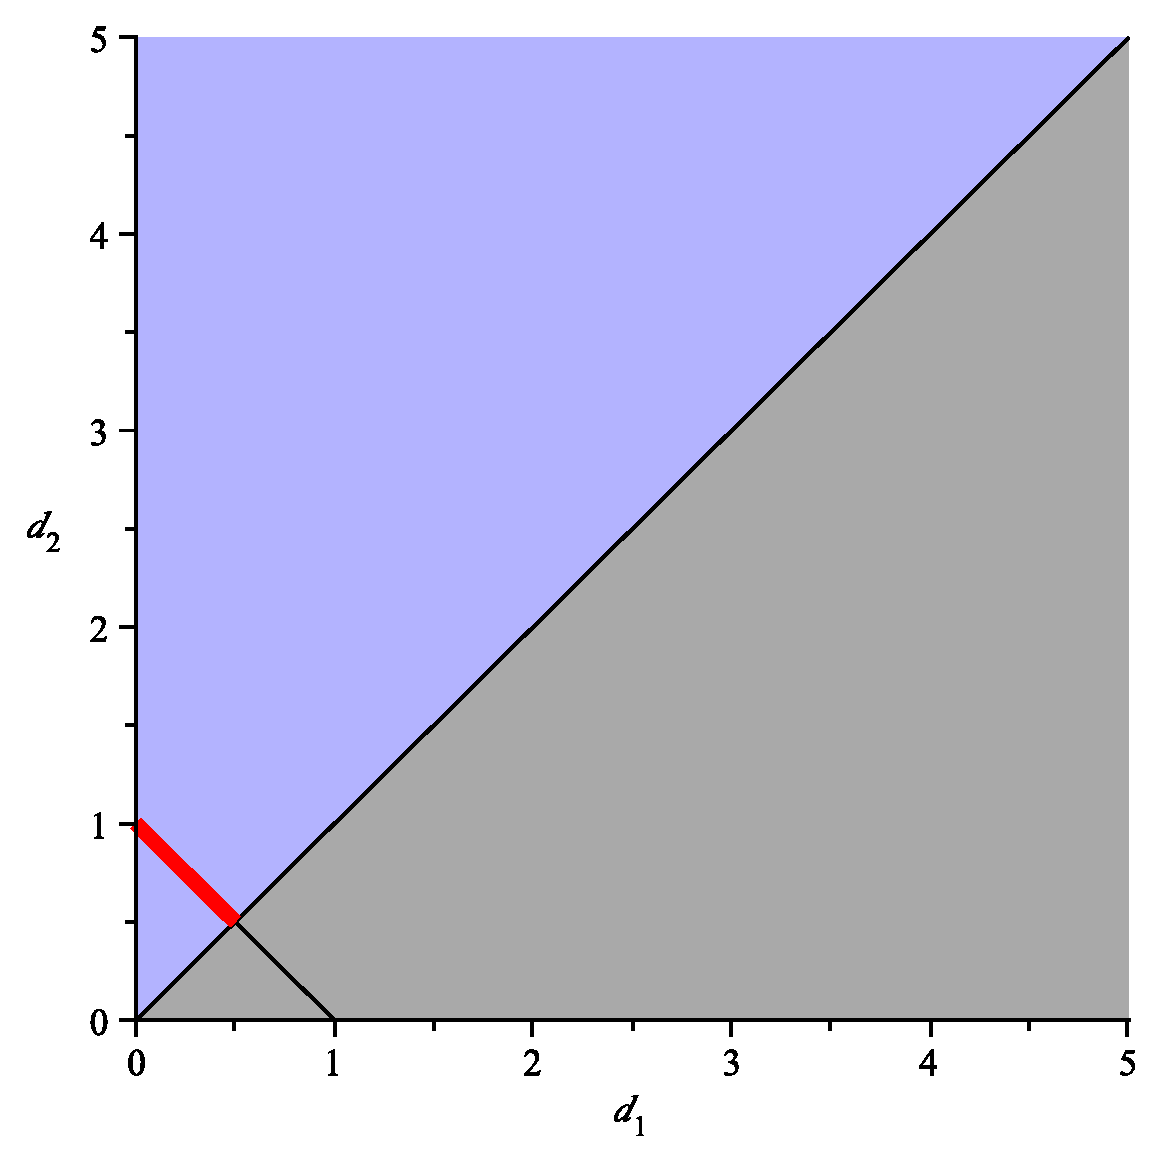
\includegraphics[scale=0.35]{DExtreme.pdf}
\caption{Visualization of the set $D$: This set really consists of the set of points on the red line. This is the line where $d_1 + d_2 = 1$ and all other constraints hold. This line has two extreme points $(0,1)$ and $(1/2,1/2)$.}
\label{fig:DExtreme}
\end{figure}
The critical part of this figure is the red line. It is the true set $D$. As a line, it has two extreme points: $(0,1)$ and $(1/2,1/2)$. Note that $(0,1)$ as an extreme point is one of the direction $[0,1]^T$ we illustrated in Example \ref{ex:UnboundedPolyhedron}.
\end{example}

\begin{exercise} Show that $\mathbf{d} = [1/2,1/2]^T$ is a direction of the polyhedral set $P$ from Example \ref{ex:UnboundedPolyhedron}. Now find a non-extreme direction (whose components sum to $1$) using the feasible region illustrated in the previous example. Show that the direction you found is a direction of the polyhedral set. Create a figure like Figure \ref{fig:UnboundedPolyhedron} to illustrate \textit{both} these directions.
\end{exercise}

\section{Caratheodory Characterization Theorem}
\begin{lemma} The polyhedral set defined by:
\begin{displaymath}
P = \left\{\mathbf{x} \in \mathbb{R}^n : \mathbf{A} \mathbf{x} \leq \mathbf{b},\;\mathbf{x} \geq \mathbf{0}\right\}
\end{displaymath}
has a finite, non-zero number of extreme points (assuming that $\mathbf{A}$ is not an empty matrix)\footnote{Thanks to Bob Pakzah-Hurson for the suggestion to improve the statement of this lemma.}.
\label{lem:FiniteExtremePoints}
\end{lemma}
\begin{proof} 
Let $\mathbf{x} \in P$. If $\mathbf{x}$ is an extreme point, then the theorem is proved. Suppose that $\mathbf{x}$ is not an extreme point. Then by Theorem \ref{thm:DefExtremePoint}, $\mathbf{x}$ lies at the intersection of $r < n$ binding constraints (where $r$ could be zero). The fact that $\mathbf{x}$ is not an extreme point of $P$ implies the existence of $\mathbf{y}_1, \mathbf{y}_2 \in P$ and a $\lambda > 0$ so that $\mathbf{x} = \lambda\mathbf{y}_1 + (1 - \lambda)\mathbf{y}_2$. For this to hold, we know that the $r$ constraints that bind at $\mathbf{x}$ must also be binding at $\mathbf{y}_1$ and $\mathbf{y}_2$.

Let $\mathbf{d} = \mathbf{y}_2 - \mathbf{y}_1$ be the direction from $\mathbf{y}_1$ to $\mathbf{y}_2$. We can see that:
\begin{equation}
\begin{aligned}
\mathbf{y}_1 = &\mathbf{x} - (1-\lambda)\mathbf{d}\\
\mathbf{y}_2 = &\mathbf{x} + \lambda\mathbf{d}
\end{aligned}
\label{eqn:Directions}
\end{equation}
The values $\mathbf{x} + \gamma\mathbf{d}$ and $\mathbf{x} - \gamma\mathbf{d}$ for $\gamma > 0$ correspond to motion from $\mathbf{x}$ along the direction of $\mathbf{d}$. From Expression \ref{eqn:Directions}, we can move in either the positive or negative direction of $\mathbf{d}$ and remain in $P$. Let $\gamma$ be the \textit{largest} value so that both $\mathbf{x} + \gamma\mathbf{d}$ or $\mathbf{x} - \gamma\mathbf{d}$ is in $P$. Clearly we cannot move in both directions infinitely far since $\mathbf{x} \geq \mathbf{0}$ and hence $\gamma < \infty$. Without loss of generality, suppose that $\gamma$ is determined by $\mathbf{x} - \gamma\mathbf{d}$. (That is, $\mathbf{x} - (\gamma + \epsilon)\mathbf{d} \not\in P$ for $\epsilon > 0$). Let $\mathbf{x}_1 = \mathbf{x} - \gamma\mathbf{d}$. Since $r$ hyperplanes are binding at $\mathbf{x}$ (and $\mathbf{y}_1$ and $\mathbf{y}_2)$ it is clear that these same hyperplanes are binding at $\mathbf{x}_1$ and at least one more (because of how we selected $\gamma$). Thus there are at least $r+1$ binding hyperplanes at $\mathbf{x}_1$. If $r+1 = n$, then we have identified an extreme point. Otherwise, we may repeat the process until we find an extreme point. 

To show that the number of extreme points is finite, we note that every extreme point is the intersection of $n$ linearly independent hyperplanes defining $P$. There are $n+m$ hyperplanes defining $P$ and therefore the number of possible extreme points is limited by $\binom{n+m}{n}$. This completes the proof.
\end{proof}

\begin{lemma} Let $P$ be a non-empty polyhedral set. Then the set of directions of $P$ is empty if and only if $P$ is bounded. 
\end{lemma}
\begin{proof} Clearly if $P$ is bounded then it cannot have a direction. If $P$ were contained in a ball $B_r(\mathbf{x}_0)$ then we know that for every $\mathbf{x} \in P$ we have $|\mathbf{x}-\mathbf{x}_0| < r$. If $\mathbf{d}$ is a direction of $P$, then we have $\mathbf{x} + \lambda\mathbf{d}$ for all $\lambda > 0$. We simply need to choose $\lambda$ large enough so that $|\mathbf{x} + \lambda\mathbf{d}-\mathbf{x}_0| > r$. 

If $P$ has no directions, then there is some absolute upper bound on the value of $|\mathbf{x}|$ for all $\mathbf{x} \in P$. Let $r$ be this value. Then trivially, $B_{r+1}(\mathbf{0})$ contains $P$ and so $P$ is bounded. 
\end{proof}

\begin{lemma} Let $P$ be a non-empty unbounded polyhedral set. Then the number extreme directions of $P$ is finite and non-zero.
\end{lemma}
\begin{proof} The result follows immediately from Theorem \ref{thm:ExtremeDirections} and Lemma \ref{lem:FiniteExtremePoints}. 
\end{proof}

\begin{theorem} Let $P$ be a non-empty, unbounded polyhedral set defined by:
\begin{displaymath}
P = \left\{\mathbf{x} \in \mathbb{R}^n : \mathbf{A} \mathbf{x} \leq \mathbf{b},\;\mathbf{x} \geq \mathbf{0}\right\}
\end{displaymath}
(where we assume $\mathbf{A}$ is not an empty matrix). Suppose that $P$ has extreme points $\mathbf{x}_1,\dots,\mathbf{x}_k$ and extreme directions $\mathbf{d_1},\dots,\mathbf{d}_l$. If $\mathbf{x} \in P$, then there exists constants $\lambda_1,\dots,\lambda_k$ and $\mu_1,\dots,\mu_l$
such that:
\begin{equation}
\begin{aligned}
\mathbf{x} = &\sum_{i=1}^{k}\lambda_i\mathbf{x}_i + \sum_{j=1}^{l}\mu_j\mathbf{d}_j\\
&\sum_{i=1}^k \lambda_i = 1\\
&\lambda_i \geq 0\;\;i=1,\dots,k\\
&\mu_j \geq 0\;\;1,\dots,l
\end{aligned}
\label{eqn:Representation}
\end{equation}
\end{theorem}
\begin{proof}
Let $\mathbf{x} \in P$. We will show that we can identify $\lambda_1,\dots,\lambda_k$ and $\mu_1,\dots,\mu_l$ making Expression \ref{eqn:Representation} true. Define the set:
\begin{equation}
\overline{P} = P \cap \{\mathbf{x} \in \mathbb{R}^n : \mathbf{e}^T\mathbf{x} \leq M\}
\end{equation}
where $M$ is a large constant so that $\mathbf{e}^T\mathbf{x}_i < M$ for $i=1,\dots,k$ and $\mathbf{e}^T\mathbf{x} < M$. That is, $M$ is large enough so that the sum of the components of any extreme point is less than $M$ and the sum of the components of $\mathbf{x}$ is less than $M$.

It is clear that $\overline{P}$ is bounded. In fact, if $P$ is bounded, then $\overline{P} = P$. Furthermore $\overline{P}$ is a polyhedral set contained in $P$ and therefore the extreme points of $P$ are also the extreme points of $\overline{P}$. Define 
\begin{displaymath}
\overline{E}_p = \{\mathbf{x}_1,\dots,\mathbf{x}_k,\dots,\mathbf{x}_{k+u}\}
\end{displaymath}
as the extreme points of $\overline{P}$. By Theorem \ref{lem:FiniteExtremePoints} we know that $0 \leq u < \infty$. If $\mathbf{x} \in \overline{E}_p$, then $\mathbf{x}$ can be written as a convex combination of the elements of $\overline{E}_p$. Therefore, assume that $\mathbf{x} \not\in \overline{E}_p$. Now, suppose that the system of equations $\mathbf{G}\mathbf{y} = \mathbf{g}$ represents the binding hyperplanes (constraints) of $\overline{P}$ that are active at $\mathbf{x}$. Clearly $\mathrm{rank}(\mathbf{G}) < n$ (otherwise, $\mathbf{x}$ would be an extreme point of $\overline{E}_p$).

Let $\mathbf{d} \neq 0$ be a solution to the problem $\mathbf{G}\mathbf{d} = 0$ and compute $\gamma_1 = \max\{\gamma : \mathbf{x} + \gamma\mathbf{d} \in \overline{X}\}$. Since $\overline{X}$ is bounded and $\mathbf{x}$ is not in $\overline{E}_p$, then $0 < \gamma_1 < \infty$. Let $\mathbf{y} = \mathbf{x} + \gamma_1\mathbf{d}$. Just as in the proof of Lemma \ref{lem:FiniteExtremePoints}, at $\mathbf{y}$, we now have (at least one) additional linearly independent binding hyperplane of $\overline{P}$. If there are now $n$ binding hyperplanes, then $\mathbf{y}$ is an extreme point of $\overline{P}$. Otherwise, we may repeat this process until we identify such an extreme point. Let $\mathbf{y}_1$ be this extreme point. Clearly $\mathbf{G}\mathbf{y}_1 = \mathbf{g}$. Now define:
\begin{displaymath}
\gamma_2 = \max\{\gamma : \mathbf{x} + \gamma(\mathbf{x} - \mathbf{y}_1) \in \overline{P}\}
\end{displaymath}
The value value $\mathbf{x} - \mathbf{y}_1$ is the direction from $\mathbf{y}_1$ to $\mathbf{x}$ and $\gamma_2$ may be thought of as the size of a step that one can from $\mathbf{x}$ away from $\mathbf{y}_1$ along the line from $\mathbf{y}_1$ to $\mathbf{x}$. Let
\begin{equation}
\mathbf{y}_2 = \mathbf{x} + \gamma_2(\mathbf{x} - \mathbf{y}_1)
\label{eqn:Defy2}
\end{equation}
Again $\gamma_2 < \infty$ since $\overline{P}$ is bounded and further $\gamma_2 > 0$ since:
\begin{equation}
\mathbf{G}\left(\mathbf{x} + \gamma_2(\mathbf{x} - \mathbf{y}_1\right) = \mathbf{g}
\end{equation}
for all $\gamma \geq 0$ (as $\mathbf{G}\mathbf{x} = \mathbf{G}\mathbf{y}_1$). As we would expect, $\mathbf{G}\mathbf{y}_2 = \mathbf{g}$ and there is at least one additional hyperplane binding at $\mathbf{y}_2$ (as we saw in the proof of Lemma \ref{lem:FiniteExtremePoints}). Trivially, $\mathbf{x}$ is a convex combination of $\mathbf{y}_1$ and $\mathbf{y}_2$. Specifically, let 
\begin{displaymath}
\mathbf{x} = \delta\mathbf{y}_1 + (1-\delta)\mathbf{y}_2
\end{displaymath}
with $\delta \in (0,1)$ and $\delta = \gamma_2/(1 + \gamma_2)$. This follows from Equation \ref{eqn:Defy2}, by solving for $\mathbf{x}$. Now if $\mathbf{y}_2 \in \overline{E}_p$, then we have written $\mathbf{x}$ as a convex combination of extreme points of $\overline{P}$. Otherwise, we can repeat the process we used to find $\mathbf{y}_2$ in terms of $\mathbf{y}_3$ and $\mathbf{y}_4$, at which an additional hyperplane (constraint) is binding. We may repeat this process until we identify elements of $\overline{E}_P$. Reversing this process, we can ultimately write $\mathbf{x}$ as a convex combination of these extreme points. Thus we have shown that we can express $\mathbf{x}$ as a convex combination of the extreme points of $\overline{E}_P$. 

Based on our deduction, we may write:
\begin{equation}
\begin{aligned}
\mathbf{x} = & \sum_{i=1}^{k + u}\delta_i\mathbf{x}_i\\
1 = & \sum_{i=1}^{k+u}\delta_i\\
& \delta_i \geq 0\;\;i=1,\dots,k+u
\end{aligned}
\label{eqn:PenUlt}
\end{equation}
If $\delta_i = 0$ if $i > k$, then we have succeeded in expressing $\mathbf{x}$ as a convex combination of the extreme points of $P$. Suppose not. Consider $\mathbf{x}_v$ with $v > k$ (so $\mathbf{x}_v$ is an extreme point of $\overline{P}$ but not $P$). Then it follows that $\mathbf{e}^T\mathbf{x}_v = M$ must hold (otherwise, $\mathbf{x}_v$ is an extreme point of $P$). Since there are $n$ binding hyperplanes at $\mathbf{x}_v$, there must be $n-1$ hyperplanes defining $P$ binding at $\mathbf{x}_v$. Thus, there is an edge connecting $\mathbf{x}_v$ and some extreme point of $P$ (i.e., there is an extreme point of $P$ that shares $n-1$ binding hyperplanes with $\mathbf{x}_v$). Denote this extreme point as $\mathbf{x}_{i(v)}$; it is adjacent to $\mathbf{x}_v$.  Consider the direction $\mathbf{x}_v - \mathbf{x}_{v(i)}$. This must be a recession direction of $P$ since there is no other hyperplane that binds in this direction before $\mathbf{e}^T\mathbf{x} = M$. Define:
\begin{displaymath}
\theta_v = \mathbf{e}^T(\mathbf{x}_v - \mathbf{x}_{v(i)})
\end{displaymath}
and let
\begin{displaymath}
\mathbf{d} = \frac{\mathbf{x}_v - \mathbf{x}_{v(i)}}{\theta_v}
\end{displaymath}
then $\mathbf{e}^T\mathbf{d} = 1$ as we have normalized the direction elements and therefore $\mathbf{d} \in D$. Again, let $\mathbf{G}\mathbf{y} = \mathbf{g}$ be the system of $n-1$ binding linear hyperplanes shared by $\mathbf{x}_v$ and $\mathbf{x}_{v(i)}$. Then trivially:
\begin{displaymath}
\mathbf{G}(\mathbf{x}_v - \mathbf{x}_{v(i)}) = \mathbf{G}\mathbf{d} = 0
\end{displaymath}
and therefore, there are $n-1$ linearly independent binding hyperplanes in the system $\mathbf{A}\mathbf{d} \leq 0$, $\mathbf{d} \geq 0$. At last we see that with $\mathbf{e}^T\mathbf{d} = 1$ that $\mathbf{d}$ must be an extreme point of $D$ and therefore an extreme direction of $P$. Let $\mathbf{d}_{j(v)} = \mathbf{d}$ be this extreme direction. Thus we have:
\begin{displaymath}
\mathbf{x}_v = \mathbf{x}_{i(v)} + \theta_v\mathbf{d}_{j(v)}
\end{displaymath}
At last we can see that by substituting this into Expression \ref{eqn:PenUlt} for each such $v$ and arbitrarily letting $i(v) = j(v) = 1$ if $\delta_v = 0$ (in which case it doesn't matter), we obtain:
\begin{equation}
\mathbf{x} = \sum_{i=1}^k\delta_j\mathbf{x}_j + \sum_{v=k+1}^{k+u}\delta_v\mathbf{x}_{i(v)} + \sum_{v=k+1}^{k+u}\delta_v\theta_v\mathbf{d}_{j(v)}
\end{equation}
We have now expressed $\mathbf{x}$ as desired. This completes the proof.
\end{proof}

\begin{example} The Cartheodory Characterization Theorem is illustrated for a bounded and unbounded polyhedral set in Figure \ref{fig:Carth}.
\begin{figure}[htbp]
\centering
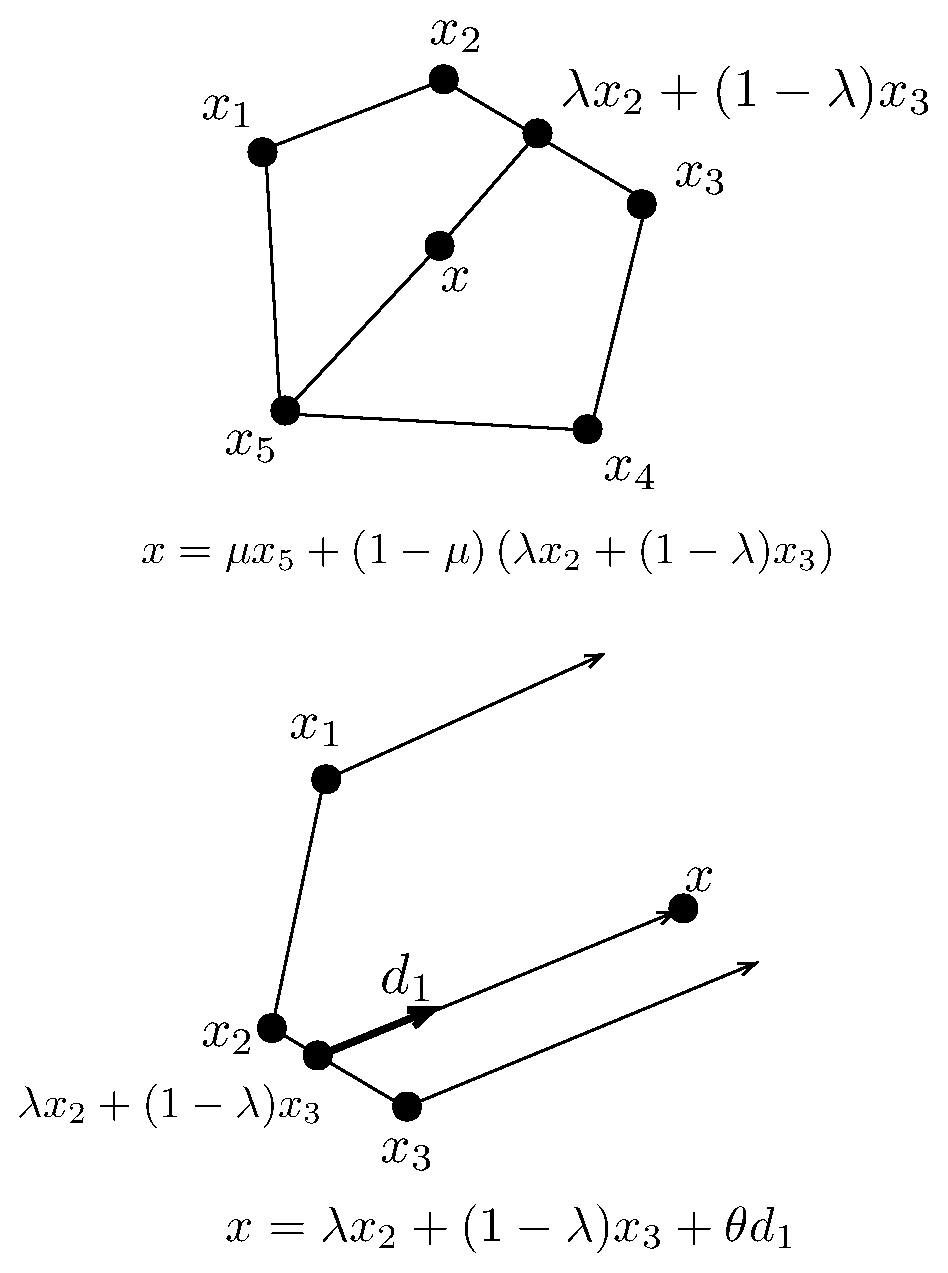
\includegraphics[scale=0.35]{Cartheodoary.pdf}
\caption{The Cartheodory Characterization Theorem: Extreme points and extreme directions are used to express points in a bounded and unbounded set.}
\label{fig:Carth}
\end{figure}
This example illustrates simply how one could construct an expression for an arbitrary point $\mathbf{x}$ inside a polyhedral set in terms of extreme points and extreme directions.
\end{example}

\chapter{The Simplex Method}
\section{Linear Programming and Extreme Points}
In this section we formalize the intuition we've obtained in all our work in two dimensional linear programming problems. Namely, we noted that if an optimal solution existed, then it occurred at an extreme point. For the remainder of this chapter, assume that $A \in \mathbb{R}^{m \times n}$ with full row rank and $b \in \mathbb{R}^m$ let
\begin{equation}
X = \{\mathbf{x} \in \mathbb{R}^n : \mathbf{A}\mathbf{x} \leq \mathbf{b},\;\;\mathbf{x} \geq \mathbf{0}\}
\end{equation}
be a polyhedral set over which we will maximize the objective function $z(x_1,\dots,x_n) = \mathbf{c}^T\mathbf{x}$, where $\mathbf{c},\mathbf{x} \in \mathbb{R}^n$. That is, we will focus on the linear programming problem:
\begin{equation}P\left\{
\begin{aligned}
\max\;\;&\mathbf{c}^T\mathbf{x}\\
s.t.\;\;&\mathbf{A}\mathbf{x} \leq \mathbf{b}\\
& \mathbf{x} \geq \mathbf{0}
\end{aligned}\right.
\end{equation}

\begin{theorem} If Problem $P$ has an optimal solution, then Problem $P$ has an optimal extreme point solution.
\label{thm:EPSoln}
\end{theorem}
\begin{proof} Applying the Cartheodory Characterization theorem, we know that any point $\mathbf{x} \in X$ can be written as:
\begin{equation}
\mathbf{x} = \sum_{i=1}^k\lambda_i\mathbf{x}_i + \sum_{i=1}^l\mu_i\mathbf{d}_i
\end{equation}
where $\mathbf{x}_1,\dots\mathbf{x}_k$ are the extreme  points of $X$ and $\mathbf{d}_1,\dots,\mathbf{d}_l$ are the extreme directions of $X$ and we know that 
\begin{equation}
\begin{aligned}
\sum_{i=1}^{k}\lambda_i & = 1\\
\lambda_i, \mu_i & \geq 0\;\;\forall i
\end{aligned}
\end{equation}
We can rewrite problem $P$ using this characterization as:
\begin{equation}
\begin{aligned}
\max\;\;& \sum_{i=1}^k\lambda_i\mathbf{c}^T\mathbf{x}_i + \sum_{i=1}^l\mu_i\mathbf{c}^T\mathbf{d}_i\\
s.t.\;\; & \sum_{i=1}^{k}\lambda_i = 1\\
&\lambda_i, \mu_i \geq 0\;\;\forall i
\end{aligned}
\end{equation}
If there is some $i$ such that $\mathbf{c}^T\mathbf{d}_i > 0$, then we can simply choose $\mu_i$ as large as we like, making the objective as large as we like, the problem will have no finite solution. 

Therefore, assume that $\mathbf{c}^T\mathbf{d}_i \leq 0$ for all $i=1,\dots,l$ (in which case, we may simply choose $\mu_i = 0$, for all $i$). Since the set of extreme points $\mathbf{x}_1,\dots\mathbf{x}_k$ is finite, we can simply set $\lambda_p = 1$ if $\mathbf{c}^T\mathbf{x}_p$ has the largest value among all possible values of $\mathbf{c}^T\mathbf{x}_i$, $i=1,\dots,k$. This is clearly the solution to the linear programming problem. Since $\mathbf{x}_p$ is an extreme point, we have shown that if $P$ has a solution, it must have an extreme point solution. 
\end{proof}
\begin{corollary} Problem $P$ has a finite solution if and only if $\mathbf{c}^T\mathbf{d}_i \leq 0$ for all $i=1,\dots l$ when $\mathbf{d}_1,\dots,\mathbf{d}_l$ are the extreme directions of $X$.
\label{cor:OptimalityDirections}
\end{corollary}
\begin{proof} This is implicit in the proof of the theorem.
\end{proof}
\begin{corollary} Problem $P$ has alternative optimal solutions if there are at least two extreme points $\mathbf{x}_p$ and $\mathbf{x}_q$ so that $\mathbf{c}^T\mathbf{x}_p = \mathbf{c}^T\mathbf{x}_q$ and so that $\mathbf{x}_p$ is the extreme point solution to the linear programming problem.
\end{corollary}
\begin{proof} Suppose that $\mathbf{x}_p$ is the extreme point solution to $P$ identified in the proof of the theorem. Suppose $\mathbf{x}_q$ is another extreme point solution with $\mathbf{c}^T\mathbf{x}_p = \mathbf{c}^T\mathbf{x}_q$. Then every convex combination of $\mathbf{x}_p$ and $\mathbf{x}_q$ is contained in $X$ (since $X$ is convex). Thus every $\mathbf{x}$ with form $\lambda\mathbf{x}_p + (1-\lambda)\mathbf{x}_q$ and $\lambda \in [0,1]$ has objective function value:
\begin{displaymath}
\lambda\mathbf{c}^T\mathbf{x}_p + (1-\lambda)\mathbf{c}^T\mathbf{x}_q = 
\lambda\mathbf{c}^T\mathbf{x}_p + (1-\lambda)\mathbf{c}^T\mathbf{x}_p = 
\mathbf{c}^T\mathbf{x}_p
\end{displaymath}
which is the optimal objective function value, by assumption.
\end{proof}

\begin{exercise} Let $X = \{\mathbf{x} \in \mathbb{R}^n : \mathbf{A}\mathbf{x} \leq \mathbf{b},\;\;\mathbf{x} \geq \mathbf{0}\}$ and suppose that $\mathbf{d}_1,\dots\mathbf{d}_l$ are the extreme directions of $X$ (assuming it has any). Show that the problem:
\begin{equation}
\begin{aligned}
\min\;\;&\mathbf{c}^T\mathbf{x}\\
s.t.\;\;&\mathbf{A}\mathbf{x} \leq \mathbf{b}\\
& \mathbf{x} \geq \mathbf{0}
\end{aligned}
\end{equation}
has a finite optimal solution if (and only if) $\mathbf{c}^T\mathbf{d}_j \geq 0$ for $k=1,\dots,l$. [Hint: Modify the proof above using the Cartheodory characterization theorem.] 
\label{exer:MinDirections}
\end{exercise}

\section{Algorithmic Characterization of Extreme Points}
In the previous sections we showed that if a linear programming problem has a solution, then it must have an extreme point solution. The challenge now is to identify some simple way of identifying extreme points. To accomplish this, let us now assume that we write $X$ as:
\begin{equation}
X = \{\mathbf{x} \in \mathbb{R}^n : \mathbf{A}\mathbf{x} = \mathbf{b},\;\;\mathbf{x} \geq \mathbf{0}\}
\end{equation}
Our work in the previous sections shows that this is possible. Recall we can separate $\mathbf{A}$ into an $m\times m$ matrix $B$ and an $m \times (n-m)$ matrix $N$ and we have the result:
\begin{equation}
\mathbf{x}_\mathbf{B} = \mathbf{B}^{-1}\mathbf{b} - \mathbf{B}^{-1}\mathbf{N}\mathbf{x}_\mathbf{N}
\label{eqn:BasicVars2}
\end{equation}
We know that $\mathbf{B}$ is invertible since we assumed that $\mathbf{A}$ had full row rank. If we assume that $\mathbf{x}_\mathbf{N} = \mathbf{0}$, then the solution
\begin{equation}
\mathbf{x}_\mathbf{B} = \mathbf{B}^{-1}\mathbf{b}
\end{equation}
was called a \textit{basic solution} (See Definition \ref{def:BasicSoln}.) Clearly any basic solution satisfies the constraints $\mathbf{A}\mathbf{x} = \mathbf{b}$ but it may not satisfy the constraints $\mathbf{x} \geq \mathbf{0}$. 

\begin{definition}[Basic Feasible Solution] If $\mathbf{x}_\mathbf{B} = \mathbf{B}^{-1}\mathbf{b}$ and $\mathbf{x}_\mathbf{N} = \mathbf{0}$ is a basic solution to $\mathbf{A}\mathbf{x} = \mathbf{b}$ and $\mathbf{x}_\mathbf{B} \geq 0$, then the solution $(\mathbf{x}_\mathbf{B},\mathbf{x}_\mathbf{N})$ is called \textit{basic feasible solution}.
\end{definition}

\begin{theorem} Every basic feasible solution is an extreme point of $X$. Likewise, every extreme point is characterized by a basic feasible solution of $\mathbf{A}\mathbf{x} = \mathbf{b}, \mathbf{x} \geq \mathbf{0}$.
\label{thm:BFSEP}
\end{theorem}
\begin{proof} Since $\mathbf{A}\mathbf{x} = \mathbf{B}\mathbf{x}_\mathbf{B} + \mathbf{N}\mathbf{x}_\mathbf{N} = \mathbf{b}$ this represents the intersection of $m$ linearly independent hyperplanes (since the rank of $\mathbf{A}$ is $m$). The fact that $\mathbf{x}_\mathbf{N} = \mathbf{0}$ and $\mathbf{x_N}$ contains $n-m$ variables, then we have $n-m$ binding, linearly independent hyperplanes in $\mathbf{x}_\mathbf{N} \geq 0$. Thus the point $(\mathbf{x}_\mathbf{B}, \mathbf{x}_\mathbf{N})$ is the intersection of $m + (n-m) = n$ linearly independent hyperplanes. By Theorem \ref{thm:DefExtremePoint} we know that $(\mathbf{x}_\mathbf{B}, \mathbf{x}_\mathbf{N})$ must be an extreme point of $X$. 

Conversely, let $\mathbf{x}$ be an extreme point of $X$. Clearly $\mathbf{x}$ is feasible and by Theorem \ref{thm:DefExtremePoint} it must represent the intersection of $n$ hyperplanes. The fact that $\mathbf{x}$ is feasible implies that $\mathbf{A}\mathbf{x} = \mathbf{b}$. This accounts for $m$ of the intersecting linearly independent hyperplanes. The remaining $n-m$ hyperplanes must come from $\mathbf{x} \geq \mathbf{0}$. That is, $n-m$ variables are zero. Let $\mathbf{x}_\mathbf{N} = \mathbf{0}$ be the variables for which $\mathbf{x} \geq \mathbf{0}$ are binding. Denote the remaining variables $\mathbf{x}_\mathbf{B}$. We can see that $\mathbf{A} = [\mathbf{B} | \mathbf{N}]$ and that $\mathbf{A}\mathbf{x} = \mathbf{B}\mathbf{x}_\mathbf{B} + \mathbf{N}\mathbf{x}_\mathbf{N} = \mathbf{b}$. Clearly, $\mathbf{x}_\mathbf{B}$ is the unique solution to $\mathbf{B}\mathbf{x}_\mathbf{B} = \mathbf{b}$ and thus $(\mathbf{x}_\mathbf{B},\mathbf{x}_\mathbf{N})$ is a basic feasible solution. 
\end{proof}

\section{The Simplex Algorithm--Algebraic Form}
In this section, we will develop the simplex algorithm algebraically. The idea behind the simplex algorithm is as follows:
\begin{enumerate*}
\item Convert the linear program to standard form.
\item Obtain an initial basic feasible solution (if possible).
\item Determine whether the basic feasible solution is optimal. If yes, stop.
\item If the current basic feasible solution is not optimal, then determine which non-basic variable (zero valued variable) should become basic (become non-zero) and which basic variable (non-zero valued variable) should become non-basic (go to zero) to make the objective function value better. 
\item Determine whether the problem is unbounded. If yes, stop.
\item If the problem doesn't seem to be unbounded at this stage, find a new basic feasible solution from the old basic feasible solution. Go back to Step 3. 
\end{enumerate*}

Suppose we have a basic feasible solution $\mathbf{x} = (\mathbf{x_B},\mathbf{x_N})$. We can divide the cost vector $\mathbf{c}$ into its basic and non-basic parts, so we have $\mathbf{c} = [\mathbf{c_B}|\mathbf{c_N}]^T$. Then the objective function becomes:
\begin{equation}
\mathbf{c}^T\mathbf{x} = \mathbf{c}_\mathbf{B}^T\mathbf{x_B} + \mathbf{c}_\mathbf{N}^T\mathbf{x_N}
\label{eqn:Obj1}
\end{equation}
We can substitute Equation \ref{eqn:BasicVars2} into Equation \ref{eqn:Obj1} to obtain:
\begin{equation}
\mathbf{c}^T\mathbf{x} = \mathbf{c}_\mathbf{B}^T\left(\mathbf{B}^{-1}\mathbf{b} - \mathbf{B}^{-1}\mathbf{N}\mathbf{x_N}\right) + 
\mathbf{c_N}\mathbf{x_N} = 
\mathbf{c}_\mathbf{B}^T\mathbf{B}^{-1}\mathbf{b} + 
\left(\mathbf{c}_\mathbf{N}^T - \mathbf{c}_\mathbf{B}^T\mathbf{B}^{-1}\mathbf{N}\right)\mathbf{x}_N
\label{eqn:Obj2}
\end{equation}

Let $\mathcal{J}$ be the set of indices of non-basic variables. Then we can write Equation \ref{eqn:Obj2} as:
\begin{equation}
z(x_1,\dots,x_n) = \mathbf{c}_\mathbf{B}^T\mathbf{B}^{-1}\mathbf{b} + 
\sum_{j \in \mathcal{J}}\left(\mathbf{c}_j - \mathbf{c}_\mathbf{B}^T\mathbf{B}^{-1}\mathbf{A}_{\cdot j}\right)x_j
\end{equation}
Consider now the fact $x_j = 0$ for all $j \in \mathcal{J}$. Further, we can see that:
\begin{equation}
\frac{\partial z}{\partial x_j} = \mathbf{c}_j - \mathbf{c}_\mathbf{B}^T\mathbf{B}^{-1}\mathbf{A}_{\cdot j}
\end{equation}
This means that if $\mathbf{c}_j - \mathbf{c}_\mathbf{B}^T\mathbf{B}^{-1}\mathbf{A}_{\cdot j} > 0$ and we \textit{increase} $x_j$ from zero to some new value, then we will \textit{increase} the value of the objective function. For historic reasons, we actually consider the value 
$\mathbf{c}_\mathbf{B}^T\mathbf{B}^{-1}\mathbf{A}_{\cdot j} - \mathbf{c}_j$, called the \textit{reduced cost} and denote it as:
\begin{equation}
-\frac{\partial z}{\partial x_j} = z_j - c_j = \mathbf{c}_\mathbf{B}^T\mathbf{B}^{-1}\mathbf{A}_{\cdot j} - \mathbf{c}_j
\end{equation}
In a maximization problem, we chose non-basic variables $x_j$ with negative reduced cost to become basic because, in this case, $\partial z/\partial x_j$ is \textit{positive}. 

Assume we chose $x_j$, a non-basic variable to become non-zero (because $z_j - c_j < 0$). We wish to know which of the basic variables will become zero as we \textit{increase} $x_j$ away from zero. We must also be very careful that \textit{none} of the variables become negative as we do this. 

By Equation \ref{eqn:BasicVars2} we know that the only current basic variables will be affected by increasing $x_j$. Let us focus explicitly on Equation \ref{eqn:BasicVars2} where we include only variable $x_j$ (since all other non-basic variables are kept zero). Then we have:
\begin{equation}
\mathbf{x_B} = \mathbf{B}^{-1}\mathbf{b} - \mathbf{B}^{-1}\mathbf{A}_{\cdot j}x_j
\label{eqn:BasicSolnXj}
\end{equation}
Let $\overline{\mathbf{b}} = \mathbf{B}^{-1}\mathbf{b}$ be an $m \times 1$ column vector and let that $\overline{\mathbf{a}_j} = \mathbf{B}^{-1}\mathbf{A}_{\cdot j}$ be another $m \times 1$ column. Then we can write:
\begin{equation}
\mathbf{x_B} = \overline{\mathbf{b}} - \overline{\mathbf{a}}_j x_j
\end{equation}
Let $\overline{\mathbf{b}} = [\overline{b}_1,\dots\overline{b}_m]^T$ and 
$\overline{\mathbf{a}}_j = [\overline{a}_{j_1},\dots,\overline{a}_{j_m}]$, then we have:
\begin{equation}
\begin{bmatrix}
x_{B_1}\\
x_{B_2}\\
\vdots\\
x_{B_m}
\end{bmatrix} = 
\begin{bmatrix}
\overline{b}_1\\
\overline{b}_2\\
\vdots\\
\overline{b}_m
\end{bmatrix} - 
\begin{bmatrix}
\overline{a}_{j_1}\\
\overline{b}_{j_2}\\
\vdots\\
\overline{b}_{j_m}
\end{bmatrix}x_j = 
\begin{bmatrix}
\overline{b}_1 - \overline{a}_{j_1}x_j\\
\overline{b}_2 - \overline{a}_{j_2}x_j\\
\vdots\\
\overline{b}_m - \overline{a}_{j_m}x_j
\end{bmatrix} 
\end{equation}
We know (a priori) that $\overline{b}_i \geq 0$ for $i=1,\dots,m$. If $\overline{a}_{j_i} \leq 0$, then as we increase $x_j$, $\overline{b}_i - \overline{a}_{j_i} \geq 0$ no matter how large we make $x_j$. On the other hand, if $\overline{a}_{j_i} > 0$, then as we increase $x_j$ we know that $\overline{b}_i - \overline{a}_{j_i}x_j$ will get smaller and eventually hit zero. In order to ensure that \textit{all} variables remain non-negative, we cannot increase $x_j$ beyond a certain point. 

For each $i$ ($i=1,\dots,m$) such that $\overline{a}_{j_i} > 0$, the value of $x_j$ that will make $x_{B_i}$ goto $0$ can be found by observing that:
\begin{equation}
x_{B_i} = \overline{b}_i - \overline{a}_{j_i}x_j
\end{equation}
and if $x_{B_i} = 0$, then we can solve:
\begin{equation}
0 = \overline{b}_i - \overline{a}_{j_i}x_j \implies
x_j = \frac{\overline{b}_i}{\overline{a}_{j_i}}
\end{equation}
Thus, the \textit{largest possible value} we can assign $x_j$ and ensure that all variables remain positive is:
\begin{equation}
\min\left\{ \frac{\overline{b}_i}{\overline{a}_{j_i}} : i=1,\dots,m \text{ and } a_{j_i} > 0 \right\}
\label{eqn:MinRatioTest}
\end{equation}
Expression \ref{eqn:MinRatioTest} is called the \textit{minimum ratio test}. We are interested in which index $i$ is the minimum ratio.

Suppose that in executing the minimum ratio test, we find that $x_j = \overline{b}_k / \overline{a}_{j_k}$. The variable $x_j$ (which was non-basic) becomes basic and the variable $x_{\mathbf{B}_k}$ becomes non-basic. All other basic variables remain basic (and positive). In executing this procedure (of exchanging one basic variable and one non-basic variable) we have moved from one extreme point of $X$ to another. 

\begin{theorem} If $z_j - c_j \geq 0$ for all $j \in \mathcal{J}$, then the current basic feasible solution is optimal.
\label{thm:SimplixOptimality}
\end{theorem}
\begin{proof} We have already shown in Theorem \ref{thm:EPSoln} that if a linear programming problem has an optimal solution, then it occurs at an extreme point and we've shown in Theorem \ref{thm:BFSEP} that there is a one-to-one correspondence between extreme points and basic feasible solutions. If $z_j - c_j \geq 0$ for all $j \in \mathcal{J}$, then $\partial z/\partial x_j \leq 0$ for all non-basic variables $x_j$. That is, we cannot increase the value of the objective function by increasing the value of any non-basic variable. Thus, since moving to another basic feasible solution (extreme point) will not improve the objective function, it follows we must be at the optimal solution.
\end{proof}

\begin{theorem} In a maximization problem, if $\overline{a}_{j_i} \leq 0$ for all $i = 1,\dots,m$, and $z_j - c_j < 0$, then the linear programming problem is unbounded.
\label{thm:Unboundedness}
\end{theorem}
\begin{proof} The fact that $z_j - c_j < 0$ implies that increasing $x_j$ will improve the value of the objective function. Since $\overline{a}_{j_i} < 0$ for all $i = 1,\dots,m$, we can increase $x_j$ indefinitely without violating feasibility (no basic variable will ever go to zero). Thus the objective function can be made as large as we like. 
\end{proof}

\begin{remark} We should note that in executing the exchange of one basic variable and one non-basic variable, we must be \textit{very} careful to ensure that the resulting basis consist of $m$ linearly independent columns of the original matrix $\mathbf{A}$. The conditions for this are provided in Lemma \ref{lem:ExchangeLemma}. Specifically, we must be able to write the column corresponding to $x_j$, the entering variable, as a linear combination of the columns of $\mathbf{B}$ so that:
\begin{equation}
\alpha_1\mathbf{b}_1 + \dots \alpha_m\mathbf{b}_m = \mathbf{A}_{\cdot j}
\end{equation}
and further if we are exchanging $x_j$ for $\mathbf{x}_{\mathbf{B}_i}$ ($i=1,\dots,m$), then $\alpha_i \neq 0$.

We can see this from the fact that $\overline{\mathbf{a}}_j = \mathbf{B}^{-1}\mathbf{A}_{\cdot j}$ and therefore:
\begin{displaymath}
\mathbf{B}\overline{\mathbf{a}}_j = \mathbf{A}_{\cdot j}
\end{displaymath}
and therefore we have:
\begin{displaymath}
\mathbf{A}_{\cdot j} = \mathbf{B}_{\cdot 1}\overline{\mathbf{a}}_{j_1} + \dots + 
\mathbf{B}_{\cdot m}\overline{\mathbf{a}}_{j_m}
\end{displaymath}
which shows how to write the column $\mathbf{A}_{\cdot j}$ as a linear combination of the columns of $\mathbf{B}$. 
\end{remark}

\begin{exercise} Consider the linear programming problem given in Exercise \ref{exer:MinDirections}. Under what conditions should a non-basic variable enter the basis? State and prove an analogous theorem to Theorem \ref{thm:SimplixOptimality} using your observation. [Hint: Use the definition of reduced cost. Remember that it is $-\partial z/\partial x_j$.]
\label{exer:MinEnteringVariable}
\end{exercise}

\begin{example} Consider the Toy Maker Problem (from Example \ref{ex:ToyMaker}). The linear programming problem given in Equation \ref{eqn:ToyMakerEx} is:
\begin{displaymath}
\left\{
\begin{aligned}
\max\;\;& z(x_1,x_2) = 7x_1 + 6x_2\\
s.t.\;\;&  3x_1 + x_2 \leq 120\\
& x_1 + 2x_2 \leq 160\\
& x_1 \leq 35\\
& x_1 \geq 0\\
& x_2 \geq 0
\end{aligned}
\right.
\end{displaymath}

We can convert this problem to standard form by introducing the slack variables $s_1$, $s_2$ and $s_3$:
\begin{displaymath}
\left\{
\begin{aligned}
\max\;\; z(x_1,x_2) = 7x_1 + 6x_2\\
s.t.\;\; 3x_1 + x_2 + s_1 = 120\\
 x_1 + 2x_2 + s_2 = 160\\
 x_1 + s_3 = 35\\
 x_1,x_2,s_1,s_2,s_3\geq 0
\end{aligned}
\right.
\end{displaymath}
which yields the matrices
\begin{displaymath}
\begin{aligned}
\mathbf{c} = \begin{bmatrix}7\\6\\0\\0\\0\end{bmatrix}\;\; & 
\mathbf{x} = \begin{bmatrix}x_1\\x_2\\s_1\\s_2\\s_3\end{bmatrix}\;\;&
\mathbf{A} = 
\begin{bmatrix} 
3 & 1 & 1 & 0 & 0\\
1 & 2 & 0 & 1 & 0\\
1 & 0 & 0 & 0 & 1
\end{bmatrix}\;\;&
\mathbf{b} = \begin{bmatrix}120\\160\\35\end{bmatrix}
\end{aligned}
\end{displaymath}
We can begin with the matrices:
\begin{displaymath}
\mathbf{B} = \begin{bmatrix}
1 & 0 & 0\\
0 & 1 & 0\\
0 & 0 & 1
\end{bmatrix}\;\;
\mathbf{N} = \begin{bmatrix}
3 & 1\\
1 & 2\\
1 & 0
\end{bmatrix}
\end{displaymath}
In this case we have:
\begin{displaymath}
\mathbf{x_B} = \begin{bmatrix}s_1\\s_2\\s_3\end{bmatrix}\;\;
\mathbf{x_N} = \begin{bmatrix}x_1\\x_2\end{bmatrix}\;\;
\mathbf{c_B} = \begin{bmatrix}0\\0\\0\end{bmatrix}\;\;
\mathbf{c_N} = \begin{bmatrix}7\\6\end{bmatrix}
\end{displaymath}
and 
\begin{displaymath}
\mathbf{B}^{-1}\mathbf{b} = \begin{bmatrix}120\\160\\35\end{bmatrix}\;\;
\mathbf{B}^{-1}\mathbf{N} = \begin{bmatrix}
3 & 1\\
1 & 2\\
1 & 0
\end{bmatrix}
\end{displaymath}
Therefore:
\begin{displaymath}
\mathbf{c}_\mathbf{B}^T\mathbf{B}^{-1}\mathbf{b} = 0 \;\;\;
\mathbf{c}_\mathbf{B}^T\mathbf{B}^{-1}\mathbf{N} = \begin{bmatrix}0 & 0\end{bmatrix}\;\;\;
\mathbf{c}_\mathbf{B}^T\mathbf{B}^{-1}\mathbf{N} - \mathbf{c_N} = 
\begin{bmatrix}-7 & -6\end{bmatrix}
\end{displaymath}
Using this information, we can compute: 
\begin{gather*}
\mathbf{c}_\mathbf{B}^T\mathbf{B}^{-1}\mathbf{A}_{\cdot 1}-\mathbf{c}_1 = -7\\
\mathbf{c}_\mathbf{B}^T\mathbf{B}^{-1}\mathbf{A}_{\cdot 2}-\mathbf{c}_2 = -6
\end{gather*}
and therefore:
\begin{displaymath}
\frac{\partial z}{\partial x_1} = 7\text{ and } \frac{\partial z}{\partial x_2} = 6
\end{displaymath}

Based on this information, we could chose either $x_1$ or $x_2$ to enter the basis and the value of the objective function would increase. If we chose $x_1$ to enter the basis, then we must determine which variable will leave the basis. To do this, we must investigate the elements of 
$\mathbf{B}^{-1}\mathbf{A}_{\cdot 1}$ and the current basic feasible solution $\mathbf{B}^{-1}\mathbf{b}$. Since each element of $\mathbf{B}^{-1}\mathbf{A}_{\cdot 1}$ is positive, we must perform the minimum ratio test on each element of $\mathbf{B}^{-1}\mathbf{A}_{\cdot 1}$. We know that $\mathbf{B}^{-1}\mathbf{A}_{\cdot 1}$ is just the first column of $\mathbf{B}^{-1}\mathbf{N}$ which is:
\begin{displaymath}
\mathbf{B}^{-1}\mathbf{A}_{\cdot 1} = \begin{bmatrix}
3\\
1\\
1
\end{bmatrix}
\end{displaymath}
Performing the minimum ratio test, we see have:
\begin{displaymath}
\min\left\{\frac{120}{3},\frac{160}{1},\frac{35}{1}\right\}
\end{displaymath}
In this case, we see that index 3 ($35/1$) is the minimum ratio. Therefore, variable $x_1$ will enter the basis and variable $s_3$ will leave the basis. The new basic and non-basic variables will be:
\begin{displaymath}
\mathbf{x_B} = \begin{bmatrix}s_1\\s_2\\x_1\end{bmatrix}\;\;
\mathbf{x_N} = \begin{bmatrix}s_3\\x_2\end{bmatrix}\;\;
\mathbf{c_B} = \begin{bmatrix}0\\0\\7\end{bmatrix}\;\;
\mathbf{c_N} = \begin{bmatrix}0\\6\end{bmatrix}
\end{displaymath}
and the matrices become:
\begin{displaymath}
\mathbf{B} = \begin{bmatrix}
1 & 0 & 3\\
0 & 1 & 1\\
0 & 0 & 1
\end{bmatrix}\;\;
\mathbf{N} = \begin{bmatrix}
0 & 1\\
0 & 2\\
1 & 0
\end{bmatrix}
\end{displaymath}
Note we have simply swapped the column corresponding to $x_1$ with the column corresponding to $s_3$ in the basis matrix $\mathbf{B}$ and the non-basic matrix $\mathbf{N}$. We will do this repeatedly in the example and we recommend the reader keep track of which variables are being exchanged and why certain columns in $\mathbf{B}$ are being swapped with those in $\mathbf{N}$. 

Using the new $\mathbf{B}$ and $\mathbf{N}$ matrices, the derived matrices are then:
\begin{displaymath}
\mathbf{B}^{-1}\mathbf{b} = \begin{bmatrix}15\\125\\35\end{bmatrix}\;\;
\mathbf{B}^{-1}\mathbf{N} = \begin{bmatrix}
-3 & 1\\
-1 & 2\\
1 & 0
\end{bmatrix}
\end{displaymath}
The cost information becomes:
\begin{displaymath}
\mathbf{c}_\mathbf{B}^T\mathbf{B}^{-1}\mathbf{b} = 245 \;\;\;
\mathbf{c}_\mathbf{B}^T\mathbf{B}^{-1}\mathbf{N} = \begin{bmatrix}7 & 0\end{bmatrix}\;\;\;
\mathbf{c}_\mathbf{B}^T\mathbf{B}^{-1}\mathbf{N} - \mathbf{c_N} = 
\begin{bmatrix}7 & -6\end{bmatrix}
\end{displaymath}
using this information, we can compute: 
\begin{gather*}
\mathbf{c}_\mathbf{B}^T\mathbf{B}^{-1}\mathbf{A}_{\cdot 5}-\mathbf{c}_5 = 7\\
\mathbf{c}_\mathbf{B}^T\mathbf{B}^{-1}\mathbf{A}_{\cdot 2}-\mathbf{c}_2 = -6
\end{gather*}

Based on this information, we can only choose $x_2$ to enter the basis to ensure that the value of the objective function increases. We can perform the minimum ration test to figure out which basic variable will leave the basis. We know that $\mathbf{B}^{-1}\mathbf{A}_{\cdot 2}$ is just the second column of $\mathbf{B}^{-1}\mathbf{N}$ which is:
\begin{displaymath}
\mathbf{B}^{-1}\mathbf{A}_{\cdot 2} = \begin{bmatrix}
1\\
2\\
0
\end{bmatrix}
\end{displaymath}
Performing the minimum ratio test, we see have:
\begin{displaymath}
\min\left\{\frac{15}{1},\frac{125}{2}\right\}
\end{displaymath}
In this case, we see that index 1 ($15/1$) is the minimum ratio. Therefore, variable $x_2$ will enter the basis and variable $s_1$ will leave the basis. The new basic and non-basic variables will be:
The new basic and non-basic variables will be:
\begin{displaymath}
\mathbf{x_B} = \begin{bmatrix}x_2\\s_2\\x_1\end{bmatrix}\;\;
\mathbf{x_N} = \begin{bmatrix}s_3\\s_1\end{bmatrix}\;\;
\mathbf{c_B} = \begin{bmatrix}6\\0\\7\end{bmatrix}\;\;
\mathbf{c_N} = \begin{bmatrix}0\\0\end{bmatrix}
\end{displaymath}
and the matrices become:
\begin{displaymath}
\mathbf{B} = \begin{bmatrix}
1 & 0 & 3\\
2 & 1 & 1\\
0 & 0 & 1
\end{bmatrix}\;\;
\mathbf{N} = \begin{bmatrix}
0 & 1\\
0 & 0\\
1 & 0
\end{bmatrix}
\end{displaymath}
The derived matrices are then:
\begin{displaymath}
\mathbf{B}^{-1}\mathbf{b} = \begin{bmatrix}15\\95\\35\end{bmatrix}\;\;
\mathbf{B}^{-1}\mathbf{N} = \begin{bmatrix}
-3 & 1\\
5 & -2\\
1 & 0
\end{bmatrix}
\end{displaymath}
The cost information becomes:
\begin{displaymath}
\mathbf{c}_\mathbf{B}^T\mathbf{B}^{-1}\mathbf{b} = 335 \;\;\;
\mathbf{c}_\mathbf{B}^T\mathbf{B}^{-1}\mathbf{N} = \begin{bmatrix}-11 & 6\end{bmatrix}\;\;\;
\mathbf{c}_\mathbf{B}^T\mathbf{B}^{-1}\mathbf{N} - \mathbf{c_N} = 
\begin{bmatrix}-11 & 6\end{bmatrix}
\end{displaymath}

Based on this information, we can only choose $s_3$ to (re-enter) the basis to ensure that the value of the objective function increases. We can perform the minimum ration test to figure out which basic variable will leave the basis. We know that $\mathbf{B}^{-1}\mathbf{A}_{\cdot 5}$ is just the fifth column of $\mathbf{B}^{-1}\mathbf{N}$ which is:
\begin{displaymath}
\mathbf{B}^{-1}\mathbf{A}_{\cdot 5} = \begin{bmatrix}
-3\\
5\\
1
\end{bmatrix}
\end{displaymath}
Performing the minimum ratio test, we see have:
\begin{displaymath}
\min\left\{\frac{95}{5},\frac{35}{1}\right\}
\end{displaymath}
In this case, we see that index 2 ($95/5$) is the minimum ratio. Therefore, variable $s_3$ will enter the basis and variable $s_2$ will leave the basis. The new basic and non-basic variables will be:
\begin{displaymath}
\mathbf{x_B} = \begin{bmatrix}x_2\\s_3\\x_1\end{bmatrix}\;\;
\mathbf{x_N} = \begin{bmatrix}s_2\\s_1\end{bmatrix}\;\;
\mathbf{c_B} = \begin{bmatrix}6\\0\\7\end{bmatrix}\;\;
\mathbf{c_N} = \begin{bmatrix}0\\0\end{bmatrix}
\end{displaymath}
and the matrices become:
\begin{displaymath}
\mathbf{B} = \begin{bmatrix}
1 & 0 & 3\\
2 & 0 & 1\\
0 & 1 & 1
\end{bmatrix}\;\;
\mathbf{N} = \begin{bmatrix}
0 & 1\\
1 & 0\\
0 & 0
\end{bmatrix}
\end{displaymath}
The derived matrices are then:
\begin{displaymath}
\mathbf{B}^{-1}\mathbf{b} = \begin{bmatrix}72\\19\\16\end{bmatrix}\;\;
\mathbf{B}^{-1}\mathbf{N} = \begin{bmatrix}
6/10 & -1/5\\
1/5 & -2/5\\
-1/5 & 2/5
\end{bmatrix}
\end{displaymath}
The cost information becomes:
\begin{displaymath}
\mathbf{c}_\mathbf{B}^T\mathbf{B}^{-1}\mathbf{b} = 544 \;\;\;
\mathbf{c}_\mathbf{B}^T\mathbf{B}^{-1}\mathbf{N} = \begin{bmatrix}11/5 & 8/5\end{bmatrix}\;\;\;
\mathbf{c}_\mathbf{B}^T\mathbf{B}^{-1}\mathbf{N} - \mathbf{c_N} = 
\begin{bmatrix}11/5 & 8/5\end{bmatrix}
\end{displaymath}
Since the reduced costs are now positive, we can conclude that we've obtained an optimal solution because no improvement is possible. The final solution then is:
\begin{displaymath}
\mathbf{x_B}^* = \begin{bmatrix}
x_2\\
s_3\\
x_1
\end{bmatrix} = \mathbf{B}^{-1}\mathbf{b} = 
\begin{bmatrix}
72\\
19\\
16
\end{bmatrix}
\end{displaymath}
Simply, we have $x_1 = 16$ and $x_2 = 72$ as we obtained in Example \ref{ex:ToyMaker}. The path of extreme points we actually took in traversing the boundary of the polyhedral feasible region is shown in Figure \ref{fig:SimplexPath}.
\begin{figure}[htbp]
\centering
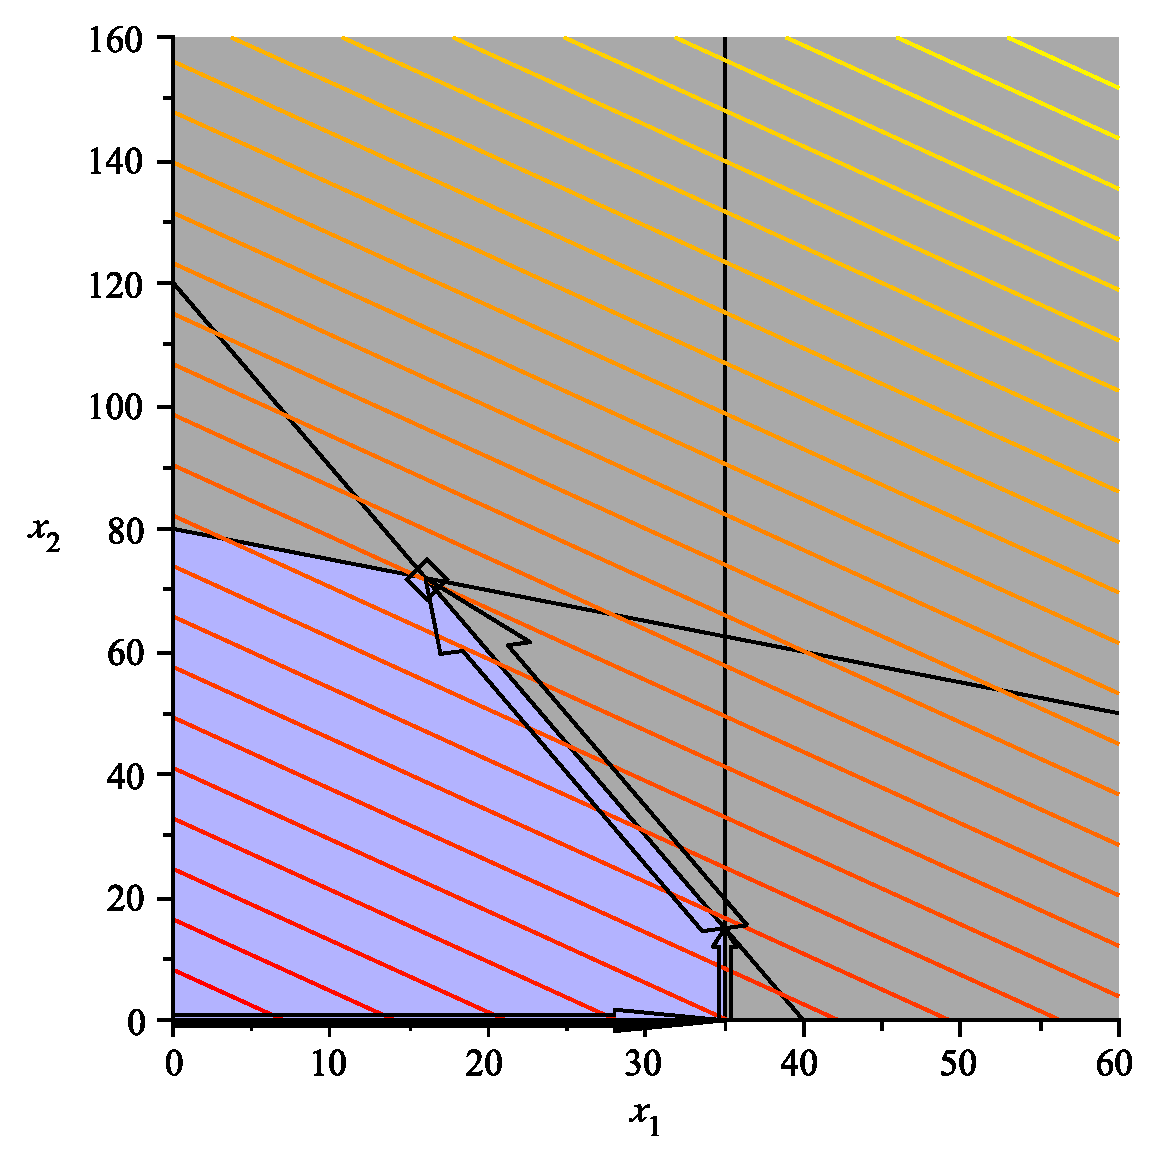
\includegraphics[scale=0.35]{SimplexPath.pdf}
\caption{The Simplex Algorithm: The path around the feasible region is shown in the figure. Each exchange of a basic and non-basic variable moves us along an edge of the polygon in a direction that increases the value of the objective function.}
\label{fig:SimplexPath}
\end{figure}
\label{ex:ToyMakerSimplex}
\end{example}

\begin{exercise} Assume that a leather company manufactures two types of belts: regular and deluxe. Each belt requires 1 square yard of leather. A regular belt requires 1 hour of skilled labor to produce, while a deluxe belt requires 2 hours of labor. The leather company receives 40 square yards of leather each week and a total of 60 hours of skilled labor is available. Each regular belt nets \$3 in profit, while each deluxe belt nets \$5 in profit. The company wishes to maximize profit. 
\begin{enumerate*}
\item Ignoring the divisibility issues, construct a linear programming problem whose solution will determine the number of each type of belt the company should produce. 

\item Use the simplex algorithm to solve the problem you stated above remembering to convert the problem to \textit{standard form} before you begin. 

\item Draw the feasible region and the level curves of the objective function. Verify that the optimal solution you obtained through the simplex method is the point at which the level curves no longer intersect the feasible region in the direction following the gradient of the objective function.
\end{enumerate*}
\label{exer:Leather}
\end{exercise}

\section{Simplex Method--Tableau Form}
No one executes the simplex algorithm in algebraic form. Instead, several representations (tableau representations) have been developed to lesson the amount of writing that needs to be done and to collect all pertinent information into a single table. 

To see how a \textit{Simplex Tableau} is derived, consider Problem $P$ in standard form:
\begin{displaymath}P\left\{
\begin{aligned}
\max\;\;&\mathbf{c}^T\mathbf{x}\\
s.t.\;\;&\mathbf{A}\mathbf{x} = \mathbf{b}\\
& \mathbf{x} \geq \mathbf{0}
\end{aligned}\right.
\end{displaymath}
We can re-write $P$ in an unusual way by introducing a new variable $z$ and separating $\mathbf{A}$ into its basic and non-basic parts to obtain:
\begin{equation}
\begin{aligned}
\max\;\;&z\\
s.t.\;\; &z - \mathbf{c}_\mathbf{B}^T\mathbf{x_B} - \mathbf{c}_\mathbf{N}^T\mathbf{x_N} = 0\\ 
&\mathbf{B}\mathbf{x_B} + \mathbf{N}\mathbf{x_N} = \mathbf{b}\\
& \mathbf{x_B},\mathbf{x_N} \geq 0
\end{aligned}
\end{equation}
From the second equation, it's clear 
\begin{equation}
\mathbf{x_B} + \mathbf{B}^{-1}\mathbf{N}\mathbf{x_N} = \mathbf{B}^{-1}\mathbf{b}
\label{eqn:Row2}
\end{equation}

We can multiply this equation by $\mathbf{c_B^T}$ to obtain:
\begin{equation}
\mathbf{c}_\mathbf{B}^T\mathbf{x_B} + \mathbf{c}_\mathbf{B}^T\mathbf{B}^{-1}\mathbf{N}\mathbf{x_N} = \mathbf{c}_\mathbf{B}^T\mathbf{B}^{-1}\mathbf{b}
\end{equation}
If we add this equation to the equation $z - \mathbf{c}_\mathbf{B}^T\mathbf{x_B} - \mathbf{c}_\mathbf{N}^T\mathbf{x_N} = 0$ we obtain:
\begin{equation}
z + \mathbf{0}^T\mathbf{x_B} + \mathbf{c}_\mathbf{B}^T\mathbf{B}^{-1}\mathbf{N}\mathbf{x_N} - \mathbf{c}_\mathbf{N}^T\mathbf{x_N} = \mathbf{c}_\mathbf{B}^T\mathbf{B}^{-1}\mathbf{b}
\end{equation}
Here $\mathbf{0}$ is the vector of zeros of appropriate size. This equation can be written as:
\begin{equation}
z + \mathbf{0}^T\mathbf{x_B} + \left(\mathbf{c}_\mathbf{B}^T\mathbf{B}^{-1}\mathbf{N} - \mathbf{c}_\mathbf{N}^T\right)\mathbf{x_N} = \mathbf{c}_\mathbf{B}^T\mathbf{B}^{-1}\mathbf{b}
\label{eqn:Row1}
\end{equation}
We can now represent this set of equations as a large matrix (or tableau):
\begin{center}
\begin{tabular}{|c|c|c|c|c|l|}
\hline
& $z$ & $\mathbf{x_B}$ & $\mathbf{x_N}$ & RHS & \\
\hline
$z$ & $1$ & $\mathbf{0}$ & $\mathbf{c}_\mathbf{B}^T\mathbf{B}^{-1}\mathbf{N} - \mathbf{c}_\mathbf{N}^T$ & $\mathbf{c}_\mathbf{B}^T\mathbf{B}^{-1}\mathbf{b}$ & Row 0\\
\hline
$\mathbf{x_B}$ & $\mathbf{0}$ & $\mathbf{1}$ & $\mathbf{B}^{-1}\mathbf{N}$ & $\mathbf{B}^{-1}\mathbf{b}$ & Rows $1$ through $m$\\
\hline
\end{tabular}
\end{center}
The augmented matrix shown within the table:
\begin{equation}
\left[
\begin{array}{ccc|c}
1 & \mathbf{0} & \mathbf{c}_\mathbf{B}^T\mathbf{B}^{-1}\mathbf{N} - \mathbf{c}_\mathbf{N}^T  & \mathbf{c}_\mathbf{B}^T\mathbf{B}^{-1}\mathbf{b}\\
\mathbf{0} & \mathbf{1} & \mathbf{B}^{-1}\mathbf{N} & \mathbf{B}^{-1}\mathbf{b}
\end{array}\right]
\end{equation}
is simply the matrix representation of the simultaneous equations described by Equations \ref{eqn:Row2} and \ref{eqn:Row1}. We can see that the first row consists of a row of the first row of the $(m+1) \times (m+1)$ identity matrix, the reduced costs of the non-basic variables and the current objective function values. The remainder of the rows consist of the rest of the $(m +1) \times (m+1)$ identity matrix, the matrix $\mathbf{B}^{-1}\mathbf{N}$ and $\mathbf{B}^{-1}\mathbf{b}$ the current non-zero part of the basic feasible solution. 

This matrix representation (or tableau representation) contains all of the information we need to execute the simplex algorithm. An entering variable is chosen from among the columns containing the reduced costs and matrix $\mathbf{B}^{-1}\mathbf{N}$. Naturally, a column with a negative reduced cost is chosen. We then chose a leaving variable by performing the minimum ratio test on the chosen column and the right-hand-side (RHS) column. We pivot on the element at the entering column and leaving row and this transforms the tableau into a new tableau that represents the new basic feasible solution.

\begin{example} Again, consider the toy maker problem. We will execute the simplex algorithm using the tableau method. Our problem in standard form is given as:
\begin{displaymath}
\left\{
\begin{aligned}
\max\;\; z(x_1,x_2) = 7x_1 + 6x_2\\
s.t.\;\; 3x_1 + x_2 + s_1 = 120\\
 x_1 + 2x_2 + s_2 = 160\\
 x_1 + s_3 = 35\\
 x_1,x_2,s_1,s_2,s_3\geq 0
\end{aligned}
\right.
\end{displaymath}
We can assume our initial basic feasible solution has $s_1$, $s_2$ and $s_3$ as basic variables and $x_1$ and $x_2$ as non-basic variables. Thus our initial tableau is simply:
\begin{equation}
\begin{array}{c}
\\
z\\
s_1\\
s_2\\
s_3
\end{array}
\left[
\begin{array}{c|ccccc|c}
z& x_1 & x_2 & s_1 & s_2 & s_3 & \text{RHS}\\
\hline
1 & -7 & -6 & 0 & 0 & 0 & 0\\
\hline
0 &  3 &  1 & 1 & 0 & 0 & 120\\
0 &  1 &  2 & 0 & 1 & 0 & 160\\
0 &  1 &  0 & 0 & 0 & 1 & 35\\
\end{array}\right]
\end{equation}
Note that the columns have been swapped so that the identity matrix is divided and $\mathbf{B}^{-1}\mathbf{N}$ is located in columns 2 and 3. This is because of our choice of basic variables. The reduced cost vector is in Row 0.

Using this information, we can see that either $x_1$ or $x_2$ can enter. We can compute the minimum ratio test (MRT) next to the RHS column. If we chose $x_2$ as the entering variable, then the MRT tells us $s_2$ will leave. We put a box around the element on which we will pivot:
\begin{equation}
\begin{array}{c}
\\
z\\
s_1\\
s_2\\
s_3
\end{array}
\left[
\begin{array}{c|ccccc|c}
z& x_1 & x_2 & s_1 & s_2 & s_3 & \text{RHS}\\
\hline
1 & -7 & -6 & 0 & 0 & 0 & 0\\
\hline
0 &  3 &  1 & 1 & 0 & 0 & 120\\
0 &  1 &  \fbox{2} & 0 & 1 & 0 & 160\\
0 &  1 &  0 & 0 & 0 & 1 & 35\\
\end{array}\right]
\begin{array}{c}
\text{MRT ($x_2$)}\\
\hline
\\
120\\
80\\
-
\end{array}
\end{equation}
If we pivot on this element, then we transform the column corresponding to $x_2$ into the identity column:
\begin{equation}
\begin{bmatrix}0 \\ 0 \\ 1 \\ 0
\end{bmatrix}
\end{equation}
This process will correctly compute the new reduced costs and $\mathbf{B}^{-1}$ matrix as well as the new cost information. The new tableau becomes:
\begin{equation}
\begin{array}{c}
\\
z\\
s_1\\
x_2\\
s_3
\end{array}
\left[
\begin{array}{c|ccccc|c}
z& x_1 & x_2 & s_1 & s_2 & s_3 & \text{RHS}\\
\hline
1 & -4 & 0 & 0 & 3 & 0 & 480\\
\hline
0 &  2.5 &  0 & 1 & -0.5 & 0 & 40\\
0 &  0.5 &  1 & 0 & 0.5 & 0 & 80\\
0 &  1 &  0 & 0 & 0 & 1 & 35\\
\end{array}\right]
\end{equation}
We can see that $x_1$ is a valid entering variable, as it has a negative reduced cost ($-4$). We can again place the minimum ratio test values on the right-hand-side of the matrix to obtain:
\begin{equation}
\begin{array}{c}
\\
z\\
s_1\\
x_2\\
s_3
\end{array}
\left[
\begin{array}{c|ccccc|c}
z& x_1 & x_2 & s_1 & s_2 & s_3 & \text{RHS}\\
\hline
1 & -4 & 0 & 0 & 3 & 0 & 480\\
\hline
0 &  \fbox{2.5} &  0 & 1 & -0.5 & 0 & 40\\
0 &  0.5 &  1 & 0 & 0.5 & 0 & 80\\
0 &  1 &  0 & 0 & 0 & 1 & 35\\
\end{array}\right]
\begin{array}{c}
\text{MRT ($x_1$)}\\
\hline
\\
16\\
160\\
35
\end{array}
\end{equation}
We now pivot on the element we have boxed to obtain the new tableau\footnote{Thanks to Ethan Wright for catching a typo here.}:
\begin{equation}
\begin{array}{c}
\\
z\\
x_1\\
x_2\\
s_3
\end{array}
\left[
\begin{array}{c|ccccc|c}
z& x_1 & x_2 & s_1 & s_2 & s_3 & \text{RHS}\\
\hline
1 & 0 & 0 & 1.6 & 2.2 & 0 & 544\\
\hline
0 &  1 &  0 & 0.4 & -0.2 & 0 & 16\\
0 &  0 &  1 & -0.2 & 0.6 & 0 & 72\\
0 &  0 &  0 & -0.4 & 0.2 & 1 & 19\\
\end{array}\right]
\end{equation}
All the reduced costs of the non-basic variables ($s_1$ and $s_2$) are positive and so this is the optimal solution to the linear programming problem. We can also see that this solution agrees with our previous computations on the Toy Maker Problem.
\end{example}

\section{Identifying Unboundedness}
We have already identified a theorem for detecting unboundedness. Recall Theorem \ref{thm:Unboundedness}:
\textit{In a maximization problem, if $\overline{a}_{j_i} < 0$ for all $i = 1,\dots,m$, and $z_j - c_j < 0$, then the linear programming problem is unbounded.}

This condition occurs when a variable $x_j$ should enter the basis because $\partial{z}/\partial{x_j} > 0$ and there is no blocking basis variable. That is, we can arbitrarily increase the value of $x_j$ without causing any variable to become negative. We give an example:
\begin{example} Consider the Linear programming problem from Example \ref{ex:LPUnboundFeasibleRegion1}:
\begin{displaymath}
\left\{
\begin{aligned}
\max\;\;& z(x_1,x_2) = 2x_1 - x_2\\
s.t.\;\;& x_1 - x_2 \leq 1\\
& 2x_1 + x_2 \geq 6\\
&x_1,x_2 \geq 0
\end{aligned}
\right.
\end{displaymath}
We can convert this problem into standard form by adding a slack variable $s_1$ and a surplus variable $s_2$:
\begin{displaymath}
\left\{
\begin{aligned}
\max\;\;& z(x_1,x_2) = 2x_1 - x_2\\
s.t.\;\;& x_1 - x_2 + s_1 = 1\\
& 2x_1 + x_2 - s_2 = 6\\
&x_1,x_2,s_1,s_2 \geq 0
\end{aligned}
\right.
\end{displaymath}

This yields the matrices:
\begin{displaymath}
\mathbf{c} = \begin{bmatrix}2 \\ -1 \\ 0 \\ 0\end{bmatrix}\;\;
\mathbf{x} = \begin{bmatrix}x_1 \\ x_2 \\ s_1 \\ s_2\end{bmatrix}\;\;
\mathbf{A} = \begin{bmatrix} 
1 & -1 & 1 & 0\\
2 & 1 & 0 & -1
\end{bmatrix}\;\;
\mathbf{b} = \begin{bmatrix}1 \\ 6\end{bmatrix}
\end{displaymath}
We have both slack and surplus variables, so the case when $x_1 = x_2 = 0$ is not a valid initial solution. We can chose a valid solution based on our knowledge of the problem. Assume that $s_1 = s_2 = 0$ and so we have:
\begin{displaymath}
\mathbf{B} = \begin{bmatrix}
1 & -1\\
2 & 1
\end{bmatrix}\;\;
\mathbf{N} = \begin{bmatrix}
1 & 0\\
0 & -1
\end{bmatrix}
\end{displaymath}
In this case we have:
\begin{displaymath}
\mathbf{x_B} = \begin{bmatrix}x_1 \\ x_2\end{bmatrix}\;\;
\mathbf{x_N} = \begin{bmatrix}s_1 \\ s_2\end{bmatrix}\;\;
\mathbf{c_B} = \begin{bmatrix}2 \\ -1\end{bmatrix}\;\;
\mathbf{c_N} = \begin{bmatrix}0 \\ 0\end{bmatrix}\;\;
\end{displaymath}
This yields:
\begin{displaymath}
\mathbf{B}^{-1}\mathbf{b} = \begin{bmatrix}7/3 \\ 4/3\end{bmatrix}\;\;
\mathbf{B}^{-1}\mathbf{N} = \begin{bmatrix}1/3 & -1/3 \\ -2/3 & -1/3\end{bmatrix}\;\;
\end{displaymath}
We also have the cost information:
\begin{displaymath}
\mathbf{c_B}\mathbf{B}^{-1}\mathbf{b} = \frac{10}{3}\;\;
\mathbf{c_B}\mathbf{B}^{-1}\mathbf{N} = \begin{bmatrix}\frac{4}{3} & -\frac{1}{3}
\end{bmatrix}\;\;
\mathbf{c_B}\mathbf{B}^{-1}\mathbf{N}-\mathbf{c_N} = \begin{bmatrix}\frac{4}{3} & -\frac{1}{3}
\end{bmatrix}\;\;
\end{displaymath}
Based on this information, we can construct the tableau for this problem as:
\begin{equation}
\begin{array}{c}
\\
z\\
x_1\\
x_2
\end{array}
\left[
\begin{array}{c|cccc|c}
z& x_1 & x_2 & s_1 & s_2 & \text{RHS}\\
\hline
1 &  0 &  0 & \frac{4}{3} & \frac{-1}{3} & \frac{10}{3}\\
\hline
0 &  1 &  0 & \frac{1}{3} & \frac{-1}{3} & \frac{7}{3}\\
0 &  0 &  1 & \frac{-2}{3} & \frac{-1}{3} & \frac{4}{3}
\end{array}\right]
\end{equation}

We see that $s_2$ should enter the basis because $\mathbf{c_B}\mathbf{B}^{-1}\mathbf{A}_{\cdot 4}-\mathbf{c}_4 < 0$. But the column corresponding to $s_2$ in the tabluau is all negative. Therefore there is no minimum ratio test. We can let $s_2$ become as large as we like and we will keep increasing the objective function without violating feasibility. 

What we have shown is that the ray with vertex
\begin{displaymath}
\mathbf{x}_0 = \begin{bmatrix}
7/3\\
4/3\\
0\\
0
\end{bmatrix}
\end{displaymath}
and direction:
\begin{displaymath}
\mathbf{d} = \begin{bmatrix}
1/3\\
1/3\\
0\\
1
\end{bmatrix}
\end{displaymath}
is entirely contained inside the polyhedral set defined by $\mathbf{A}\mathbf{x} = \mathbf{b}$. This can be see from the fact that:
\begin{displaymath}
\mathbf{x_B} = \mathbf{B}^{-1}\mathbf{b} - \mathbf{B}^{-1}\mathbf{N}\mathbf{x_N}
\end{displaymath}
When applied in this case, we have:
\begin{displaymath}
\mathbf{x_B} = \mathbf{B}^{-1}\mathbf{b} - \mathbf{B}^{-1}\mathbf{A}_{\cdot 4}s_2
\end{displaymath}
We know that
\begin{displaymath}
-\mathbf{B}^{-1}\mathbf{A}_{\cdot 4} = 
\begin{bmatrix}
1/3\\
1/3
\end{bmatrix}
\end{displaymath}
We will be increasing $s_2$ (which acts like $\lambda$ in the definition of ray) and leaving $s_1$ equal to $0$. It's now easy to see that the ray we described is contained entirely in the feasible region. This is illustrated in the original constraints in Figure \ref{fig:UnboundedFeasibleRegionSimplex}.
\begin{figure}[htbp]
\centering
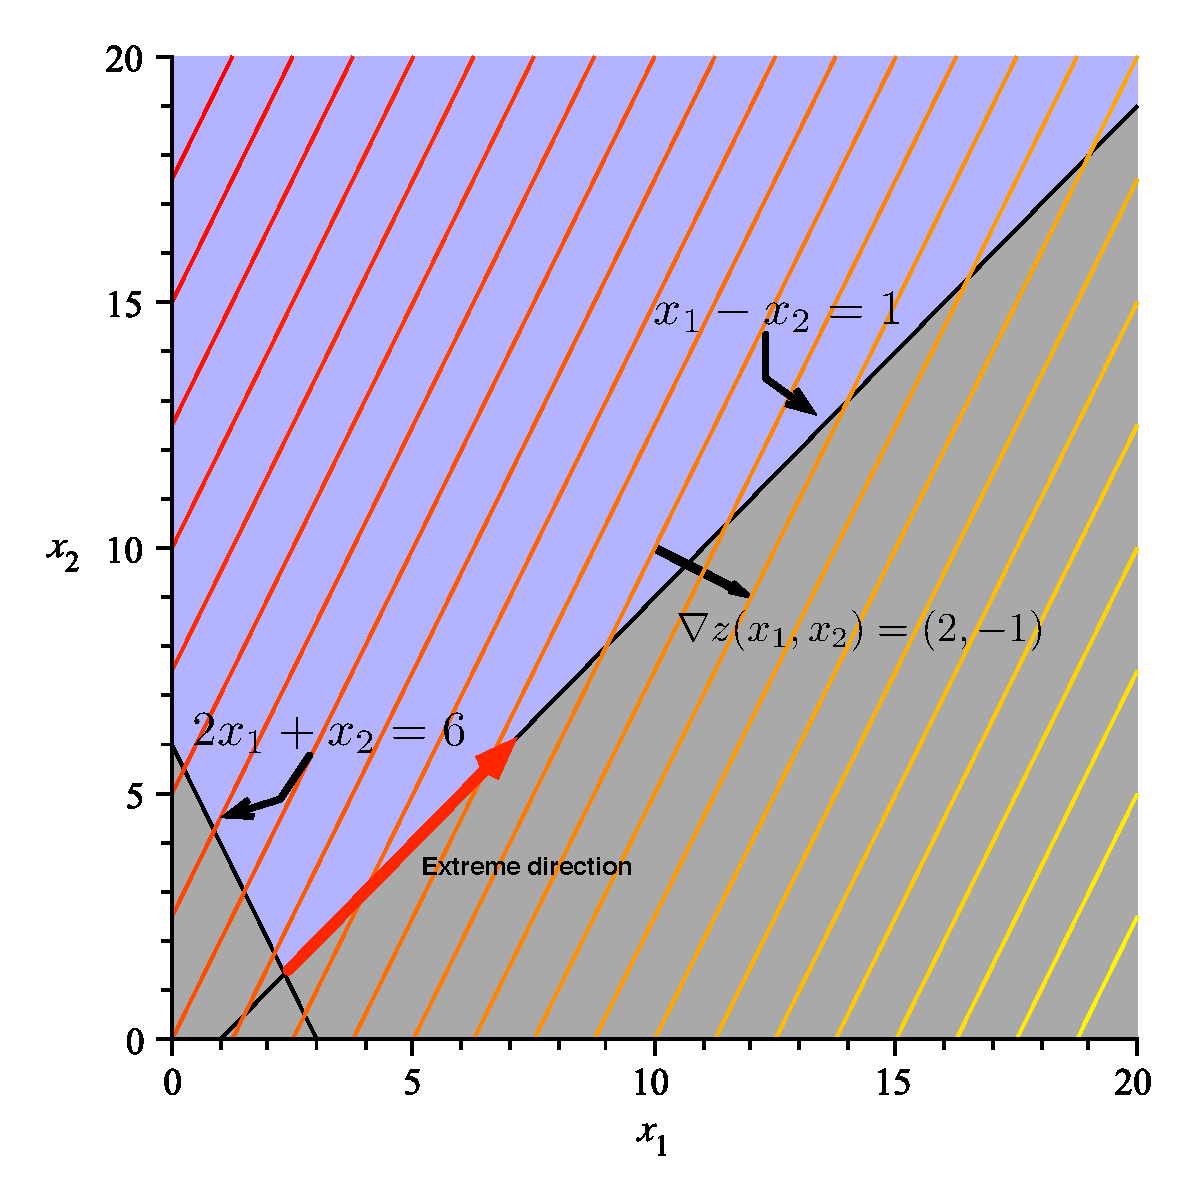
\includegraphics[scale=0.35]{UnboundedFeasibleRegionSimplex.pdf}
\caption{Unbounded Linear Program: The existence of a negative column $\overline{\mathbf{a}}_j$ in the simplex tableau for entering variable $x_j$ indicates an unbounded problem and feasible region. The recession direction is shown in the figure.}
\label{fig:UnboundedFeasibleRegionSimplex}
\end{figure}
\label{ex:UnboundedSolnSimplex}
\end{example}

Based on our previous example, we have the following theorem that extends Theorem \ref{thm:Unboundedness}:
\begin{theorem} In a maximization problem, if $\overline{a}_{j_i} \leq 0$ for all $i = 1,\dots,m$, and $z_j - c_j < 0$, then the linear programming problem is unbounded furthermore, let $\overline{\mathbf{a}}_j$ be the $j^{\text{th}}$ column of $\mathbf{B}^{-1}\mathbf{A}_{\cdot j}$ and let $\mathbf{e}_k$ be a standard basis column vector in $\mathbb{R}^{m \times (n-m)}$ where $k$ corresponds to the position of $j$ in the matrix $\mathbf{N}$. Then the direction:
\begin{equation}
\mathbf{d} = \begin{bmatrix}
-\overline{\mathbf{a}}_j\\
\mathbf{e}_k
\end{bmatrix}
\end{equation}
is an extreme direction of the feasible region $X = \{\mathbf{x} \in \mathbb{R}^n : \mathbf{A}\mathbf{x} = \mathbf{b},\;\mathbf{x} \geq \mathbf{0}\}$.
\label{thm:ExtremeDirectionSimplex} 
\end{theorem}
\begin{proof} The fact that $\mathbf{d}$ is a direction is easily verified by the fact there is an extreme point $\mathbf{x} = [\mathbf{x_B} \; \mathbf{x_N}]^T$ and for all $\lambda \geq 0$ we have:
\begin{equation}
\mathbf{x} + \lambda \mathbf{d} \in X
\end{equation}
Thus it follows from the proof of Theorem \ref{thm:DirectionChar} that $\mathbf{A}\mathbf{d} \leq \mathbf{0}$. The fact that $\mathbf{d} \geq 0$ and $\mathbf{d} \neq 0$ follows from our assumptions. Now, we know that we can write $\mathbf{A} = [\mathbf{B} | \mathbf{N}]$. Further, we know that  $\overline{\mathbf{a}}_j = \mathbf{B}^{-1}\mathbf{A}_{\cdot j}$. Let us consider $\mathbf{A}\mathbf{d}$:
\begin{equation}
\mathbf{A}\mathbf{d} = [\mathbf{B} | \mathbf{N}]\begin{bmatrix}
-\overline{\mathbf{a}}_j\\
\mathbf{e}_k
\end{bmatrix} = 
-\mathbf{B}\mathbf{B}^{-1}\mathbf{A}_{\cdot j} + \mathbf{N}\mathbf{e}_k
\end{equation}
Remember, $\mathbf{e}_k$ is the standard basis vector that has have $1$ precisely in the position corresponding to column $\mathbf{A}_{\cdot j}$ in matrix $\mathbf{N}$, so $\mathbf{A}_{\cdot j} = \mathbf{N} \mathbf{e}_j$. Thus we have:
\begin{equation}
-\mathbf{B}\mathbf{B}^{-1}\mathbf{A}_{\cdot j} + \mathbf{N}\mathbf{e}_k = 
-\mathbf{A}_{\cdot j} + \mathbf{A}_{\cdot j} = \mathbf{0}
\end{equation}
Thus, $\mathbf{A}\mathbf{d} = \mathbf{0}$. We can scale $\mathbf{d}$ so that $\mathbf{e}^T\mathbf{d} = 1$. We know that $n-m-1$ elements of $\mathbf{d}$ are zero (because of $\mathbf{e}_k$) and we know that $\mathbf{A}\mathbf{d} = \mathbf{0}$. Thus $\mathbf{d}$ can be made to represent the intersection of $n$-hyperplanes in $\mathbb{R}^n$. Thus, $\mathbf{d}$ is an extreme point of the polyhedron $D = \{\mathbf{d} \in \mathbb{R}^n : \mathbf{A}\mathbf{d} \leq \mathbf{0}, \mathbf{d}\geq \mathbf{0},\mathbf{e}^T\mathbf{d} = 1\}$. It follows from Theorem \ref{thm:ExtremeDirections}, we know that $\mathbf{d}$ is an extreme direction of $X$. 
\end{proof}

\begin{exercise} Consider the problem 
\begin{displaymath}
\left\{
\begin{aligned}
\min\;\;& z(x_1,x_2) = 2x_1 - x_2\\
s.t.\;\;& x_1 - x_2 + s_1 = 1\\
& 2x_1 + x_2 - s_2 = 6\\
&x_1,x_2,s_1,s_2 \geq 0
\end{aligned}
\right.
\end{displaymath}
Using the rule you developed in Exercise \ref{exer:MinEnteringVariable}, show that the minimization problem has an unbounded feasible solution. Find an extreme direction for this set.
[Hint: The minimum ratio test is the same for a minimization problem. Execute the simplex algorithm as we did in Example \ref{ex:UnboundedSolnSimplex} and use Theorem \ref{thm:ExtremeDirectionSimplex} to find the extreme direction of the feasible region.]
\label{exer:UnboundedMin}
\end{exercise}

\section{Identifying Alternative Optimal Solutions}
We saw in Theorem \ref{thm:SimplixOptimality} that is $z_j - c_j > 0$ for all $j \in \mathcal{J}$ (the indices of the non-basic variables), then the basic feasible solution generated by the current basis was optimal. Suppose that $z_j - c_j \geq 0$. Then we have a slightly different result:
\begin{theorem} In Problem $P$ for a given set of non-basic variables $\mathcal{J}$, if $z_j - c_j \geq 0$ for all $j \in \mathcal{J}$, then the current basic feasible solution is optimal. Further, if $z_j - c_j = 0$ for at least one $j \in \mathcal{J}$, then there are alternative optimal solutions. Furthermore, let $\overline{\mathbf{a}}_j$ be the $j^{\text{th}}$ column of $\mathbf{B}^{-1}\mathbf{A}_{\cdot j}$. Then the solutions to $P$ are:
\begin{equation} 
\left\{
\begin{aligned}
&\mathbf{x_B} = \mathbf{B}^{-1}\mathbf{b}  
-\overline{\mathbf{a}}_jx_j\\
&x_j \in \left[0,
\min\left\{
\frac{\overline{b}_i}{\overline{a}_{j_i}} : i=1,\dots,m,\;\;
\overline{a}_{j_i}>0
\right\}
\right]\\
&x_r = 0, \forall r\in\mathcal{J},\,r\neq j
\end{aligned}\right.
\label{eqn:AltOptSolnForm}
\end{equation}
\end{theorem}
\begin{proof} It follows from the proof of Theorem \ref{thm:SimplixOptimality} that the solution must be optimal as $\partial z/\partial x_j \leq 0$ for all $j \in \mathcal{J}$ and therefore increasing and $x_j$ will \textit{not} improve the value of the objective function. If there is some $j \in \mathcal{J}$ so that $z_j - c_j = 0$, then $\partial z/\partial x_j = 0$ and we may increase the value of $x_j$ up to some point specified by the minimum ratio test, while keeping other non-basic variables at zero. In this case, we will neither increase nor decrease the objective function value. Since that objective function value is optimal, it follows that the set of all such values (described in Equation \ref{eqn:AltOptSolnForm}) are alternative optimal solutions.
\end{proof}
\begin{example}
Let us consider the toy maker problem again from Example \ref{ex:ToyMaker} and \ref{ex:ToyMakerSimplex} with our adjusted objective 
\begin{equation}
z(x_1,x_2) = 18x_1 + 6x_2
\end{equation}
Now consider the penultimate basis from Example \ref{ex:ToyMakerSimplex} in which we had as basis variables $x_1$, $s_2$ and $x_2$. 
\begin{displaymath}
\mathbf{x_B} = \begin{bmatrix}x_1\\x_2\\s_2\end{bmatrix}\;\;
\mathbf{x_N} = \begin{bmatrix}s_1\\s_3\end{bmatrix}\;\;
\mathbf{c_B} = \begin{bmatrix}18\\6\\0\end{bmatrix}\;\;
\mathbf{c_N} = \begin{bmatrix}0\\0\end{bmatrix}
\end{displaymath}
The matrices become:
\begin{displaymath}
\mathbf{B} = \begin{bmatrix}
3 & 1 & 0\\
1 & 2 & 1\\
1 & 0 & 0
\end{bmatrix}\;\;
\mathbf{N} = \begin{bmatrix}
1 & 0\\
0 & 0\\
0 & 1
\end{bmatrix}
\end{displaymath}
The derived matrices are then:
\begin{displaymath}
\mathbf{B}^{-1}\mathbf{b} = \begin{bmatrix}35\\15\\95\end{bmatrix}\;\;
\mathbf{B}^{-1}\mathbf{N} = \begin{bmatrix}
0  & 1\\
1  & -3\\
-2 & 5
\end{bmatrix}
\end{displaymath}
The cost information becomes:
\begin{displaymath}
\mathbf{c}_\mathbf{B}^T\mathbf{B}^{-1}\mathbf{b} = 720 \;\;\;
\mathbf{c}_\mathbf{B}^T\mathbf{B}^{-1}\mathbf{N} = \begin{bmatrix}6 & 0\end{bmatrix}\;\;\;
\mathbf{c}_\mathbf{B}^T\mathbf{B}^{-1}\mathbf{N} - \mathbf{c_N} = 
\begin{bmatrix}6 & 0\end{bmatrix}
\end{displaymath}
This yields the tableau:
\begin{equation}
\begin{array}{c}
\\
z\\
s_1\\
s_2\\
s_3
\end{array}
\left[
\begin{array}{c|ccccc|c}
z& x_1 & x_2 & s_1 & s_2 & s_3 & \text{RHS}\\
\hline
1 &  0 & 0 & 6 & 0 & \textbf{0} & 720\\
\hline
0 &  1 & 0 & 0 & 0 & 1  		 & 35\\
0 &  0 & 1 & 1 & 0 & -3 		 & 15\\
0 &  0 & 0 & -2& 1 & 5 		 	 & 95\\
\end{array}\right]
\end{equation}

Unlike example \ref{ex:ToyMakerSimplex}, the reduced cost for $s_3$ is $0$. This means that if we allow $s_3$ to enter the basis, the objective function value will not change. Performing the minimum ratio test however, we see that $s_2$ will still leave the basis:
\begin{equation}
\begin{array}{c}
\\
z\\
x_1\\
x_2\\
s_2
\end{array}
\left[
\begin{array}{c|ccccc|c}
z& x_1 & x_2 & s_1 & s_2 & s_3 & \text{RHS}\\
\hline
1 &  0 & 0 & 6 & 0 & \textbf{0} & 720\\
\hline
0 &  1 & 0 & 0 & 0 & 1  		 & 35\\
0 &  0 & 1 & 1 & 0 & -3 		 & 15\\
0 &  0 & 0 & -2& 1 & \fbox{5} 		 	 & 95\\
\end{array}\right]
\begin{array}{c}
\text{MRT ($s_3$)}\\
\hline
\\
35\\
-\\
19
\end{array}
\end{equation}


Therefore any solution of the form:
\begin{equation}
\begin{aligned}
&s_3 \in [0,19]\\
&\begin{bmatrix}
x_1\\
x_2\\
s_2
\end{bmatrix} = 
\begin{bmatrix}35\\15\\95\end{bmatrix} - 
\begin{bmatrix}1\\-3\\5\end{bmatrix}s_3
\end{aligned}
\label{eqn:InfAltOptSimplex}
\end{equation}
is an optimal solution to the linear programming problem. This precisely describes the edge shown in Figure \ref{fig:InfiniteOptSoln2}.
\begin{figure}[htbp]
\centering
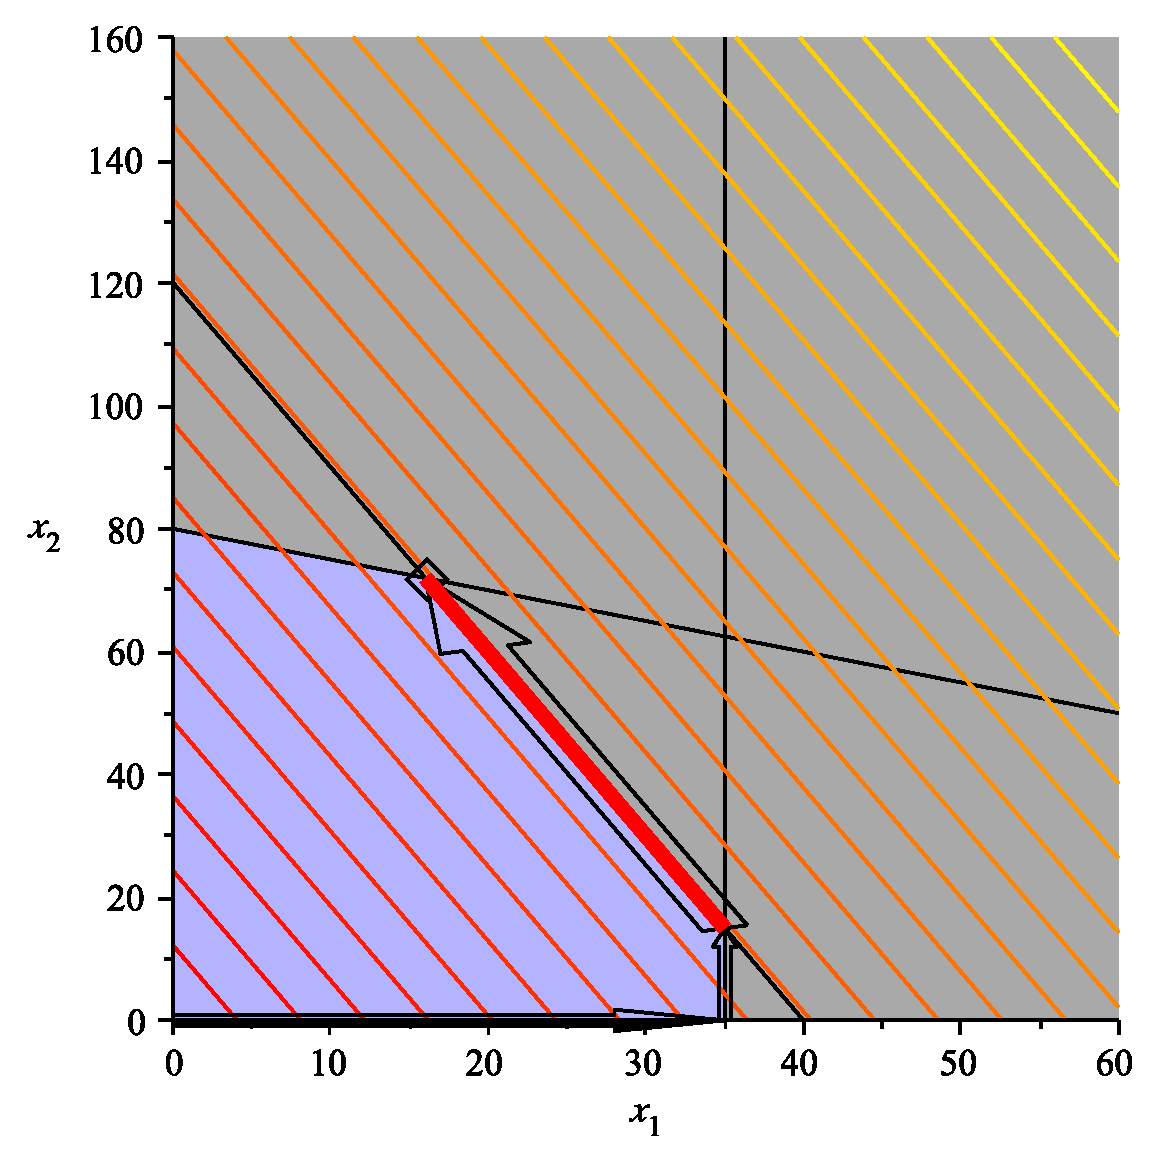
\includegraphics[scale=0.35]{InfOptSimplex.pdf}
\caption{Infinite alternative optimal solutions: In the simplex algorithm, when $z_j - c_j \geq 0$ in a maximization problem with at least one $j$ for which $z_j - c_j = 0$, indicates an infinite set of alternative optimal solutions.}
\label{fig:InfiniteOptSoln2}
\end{figure}
\end{example}

\begin{exercise} Consider the diet problem we covered in Example \ref{ex:Diet}. I wish to design a diet consisting of Raman noodles and ice cream. I'm interested in spending as little money as possible but I want to ensure that I eat at least 1200 calories per day and that I get at least 20 grams of protein per day. Assume that each serving of Raman costs \$1 and contains 100 calories and 2 grams of protein. Assume that each serving of ice cream costs \$1.50 and contains 200 calories and 3 grams of protein. 
\begin{enumerate}
\item Develop a linear programming problem that will help me minimize the cost of my food intake. 
\item Remembering to transform the linear programming problem you found above into standard form, use the simplex algorithm to show that this problem has an infinite set of alternative optimal solutions. 
\item At an optimal extreme point, find an expression for the set of infinite alternative optimal exteme points like the one shown in Equation \ref{eqn:InfAltOptSimplex}. 
\item Plot the feasible region and the level curves of the objective function. Highlight the face of the polyhedral set on which the alternative optimal solutions can be found.
\end{enumerate}

\end{exercise}

\section{Degeneracy and Convergence}
In this section we give an example of degeneracy and its impact on the simplex algorithm. 

\begin{example}
Consider the modified form of the toy maker problem originally stated in Example \ref{ex:ToyMakerDegen}:
\begin{equation}
\left\{
\begin{aligned}
\max\;\;&7x_1 + 6x_2\\
s.t.\;\;&3x_1 + x_2 \leq 120\\
&x_1 + 2x_2 \leq 160\\
&x_1 \leq 35\\
&\frac{7}{4}x_1+x_2 \leq 100\\
&x_1,x_2 \geq 0
\end{aligned}
\right.
\end{equation}
The polyhedral set and level curves of the objective function are shown Figure \ref{fig:DegenOptim}.
\begin{figure}[htbp]
\centering
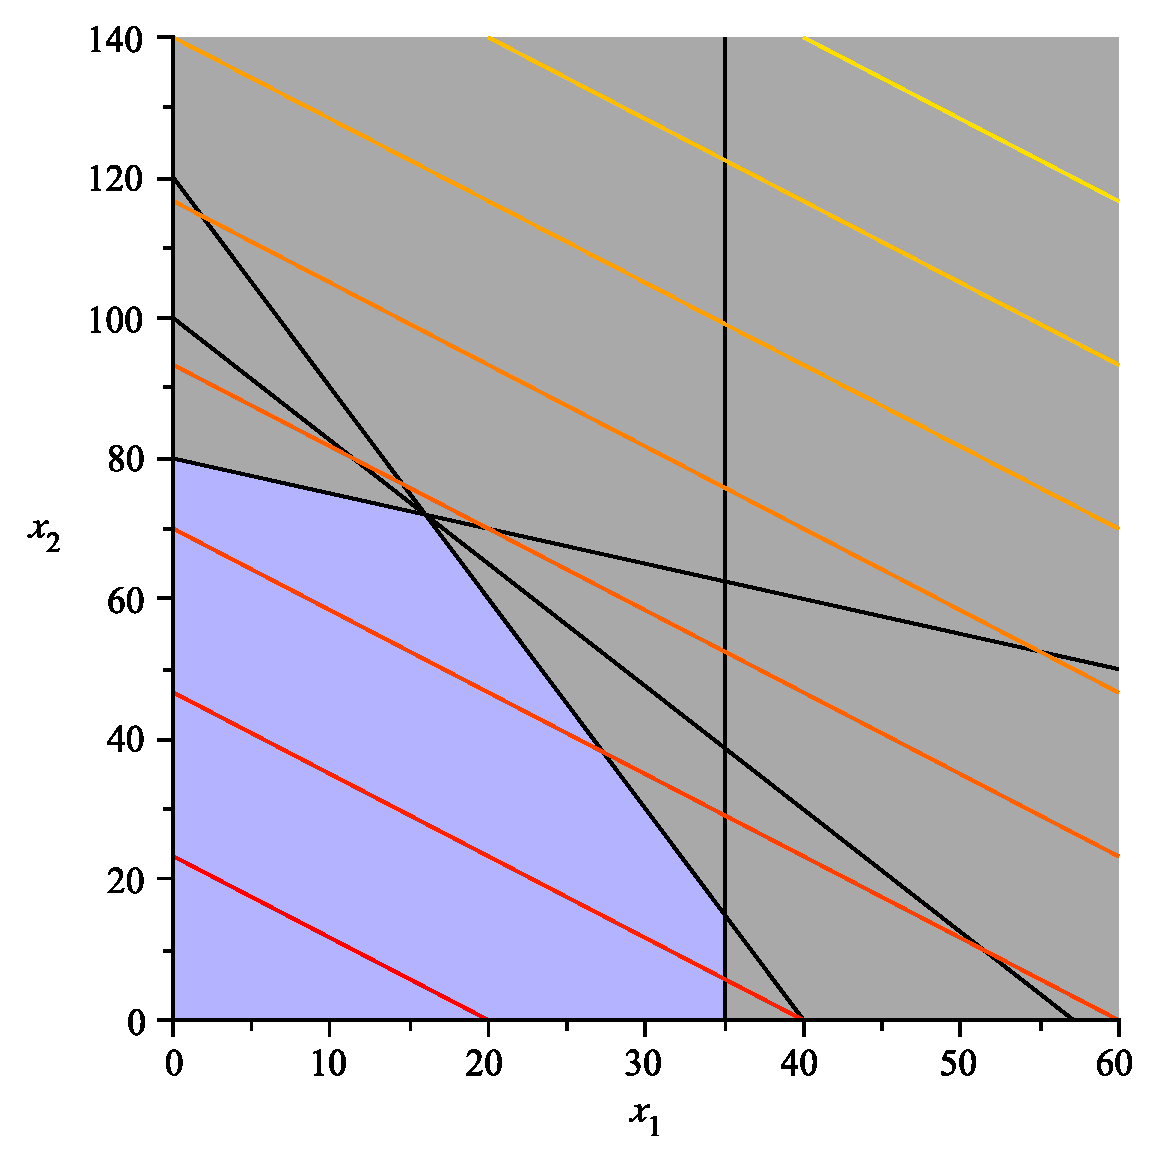
\includegraphics[scale=0.35]{DegenOptim.pdf}
\caption{An optimization problem with a degenerate extreme point: The optimal solution to this problem is still $(16,72)$, but this extreme point is degenerate, which will impact the behavior of the simplex algorithm.}
\label{fig:DegenOptim}
\end{figure}
We can convert the problem to standard form by introducing slack variables:
\begin{equation}
\left\{
\begin{aligned}
\max\;\;&7x_1 + 6x_2\\
s.t.\;\;&3x_1 + x_2 +s_1 = 120\\
&x_1 + 2x_2 + s_2 = 160\\
&x_1 + s_3 = 35\\
&\frac{7}{4}x_1+x_2 + s_4 = 100\\
&x_1,x_2,s_1,s_2,s_3,s_4 \geq 0
\end{aligned}
\right.
\end{equation}

Suppose we start at the extreme point where $x_1 = 35$ and $x_2 = 15$ and $s_2 = 95$ and $s_4 = 23.75$. In this case, the matrices are:
\begin{displaymath}
\mathbf{B} = \begin{bmatrix}
3 & 	1 & 0 & 0\\
1 & 	2 & 1 & 0\\
1 & 	0 & 0 & 0\\
7/4 & 1 & 0 & 1
\end{bmatrix}\;\;
\mathbf{N} = \begin{bmatrix}
1 & 0\\
0 & 0\\
0 & 1\\
0 & 0
\end{bmatrix}
\end{displaymath}
\begin{displaymath}
\mathbf{B}^{-1}\mathbf{b} = \begin{bmatrix}
35\\
15\\
95\\
\frac{95}{4}
\end{bmatrix}\;\;
\mathbf{B}^{-1}\mathbf{N} = \begin{bmatrix}
0 & 1\\
1 & -3\\
-2 & 5\\
-1 & \frac{5}{4}
\end{bmatrix}
\end{displaymath}
\begin{displaymath}
\mathbf{c_B}\mathbf{B}^{-1}\mathbf{b} = 335\;\;
\mathbf{c_B}\mathbf{B}^{-1}\mathbf{N} - \mathbf{c_N} = \begin{bmatrix} 6 & -11\end{bmatrix}
\end{displaymath}
The tableau representation is:
\begin{equation}
\begin{array}{c}
\\
z\\
x_1\\
x_2\\
s_2\\
s_4
\end{array}
\left[
\begin{array}{c|cccccc|c}
z& x_1 & x_2 & s_1 & s_2 & s_3 & s_4 &\text{RHS}\\
\hline
1 & 0 & 0 & 6 & 0 & -11 & 0 & 335\\
\hline
0 & 1 & 0 & 0 & 0 & 1 & 0 & 35\\
0 & 0 & 1 & 1 & 0 & -3 & 0 & 15\\
0 & 0 & 0 & -2 & 1 & 5 & 0 & 95\\
0 & 0 & 0 & -1 & 0 & \fbox{5/4} & 1 & \frac{95}{4}
\end{array}\right]
\begin{array}{c}
\text{MRT ($s_3$)}\\
\hline
\\
35\\
-\\
19\\
19
\end{array}
\end{equation}

From this, we see that the variable $s_3$ should enter (because its reduce cost is negative). In this case, there is a tie for the leaving variables: we see that $95/5 = 19 = (95/4)/(5/4)$, therefore, either $s_2$ or $s_4$ could be chosen as the leaving variable. This is because we will move to a degenerate extreme point when $s_3$ enters the basis. 

Suppose we choose $s_4$ as the leaving variable. Then our tableau will become:
\begin{equation}
\begin{array}{c}
\\
z\\
x_1\\
x_2\\
s_2\\
s_3
\end{array}
\left[
\begin{array}{c|cccccc|c}
z& x_1 & x_2 & s_1 & s_2 & s_3 & s_4 &\text{RHS}\\
\hline
1 & 0 & 0 & -14/5 & 0 & 0 & 44/5 & 544\\
\hline
0 & 1 & 0 & 4/5 			& 0 & 0  & -4/5 & 16\\
0 & 0 & 1 & -7/5 			& 0 & 0  & 12/5 & 72\\
0 & 0 & 0 & \fbox{2} 		& 1 & 0  & -4 	& 0\\
0 & 0 & 0 & -4/5 			& 0 & 1  & 4/5 	& 19
\end{array}\right]
\begin{array}{c}
\text{MRT ($s_1$)}\\
\hline
\\
20\\
-\\
0\\
-
\end{array}
\end{equation}

We now observe two things: 
\begin{enumerate*}
\item One of the basic variables ($s_2$) is zero, even though it is basic. This is \textit{the indicator} of degeneracy at an extreme point. 

\item The reduced cost of $s_1$ is negative, indicating that $s_1$ should enter the basis. 
\end{enumerate*}
If we choose $s_1$ as an entering variable, then using the minimum ratio test, we will choose $s_2$ as the leaving variable (by the minimum ratio test)\footnote{The minimum ratio test still applies when $\overline{\mathbf{b}}_{j} = 0$. In this case, we will remain at the same extreme point.}.   
Then the tableau becomes:
\begin{equation}
\begin{array}{c}
\\
z\\
x_1\\
x_2\\
s_1\\
s_3
\end{array}
\left[
\begin{array}{c|cccccc|c}
z& x_1 & x_2 & s_1 & s_2 & s_3 & s_4 &\text{RHS}\\
\hline
1 & 0 & 0 & 0 & 7/5 	& 0 & 16/5 & 544\\
\hline
0 & 1 & 0 & 0 & -2/5 		& 0  & 4/5 		& 16\\
0 & 0 & 1 & 0 & 7/10 		& 0  & -2/5 	& 72\\
0 & 0 & 0 & 1 & 1/2 		& 0  & -2 		& 0\\
0 & 0 & 0 & 0 & 2/5 		& 1  & -4/5 	& 19
\end{array}\right]
\end{equation}

Notice the objective function value $\mathbf{c_B}\mathbf{B}^{-1}\mathbf{b}$ has \textit{not} changed, because we really have not moved to a new extreme point. We have simply changed from one representation of the degenerate extreme point to another. This was to be expected, the fact that the minimum ratio was zero showed that we could not increase $s_1$ and maintain feasibility. As such $s_1 = 0$ in the new basic feasible solution. The reduced cost vector $\mathbf{c_B}\mathbf{B}^{-1}\mathbf{N} - \mathbf{c_N}$ has changed and we could now terminate the simplex method. 
\label{ex:ToyMakerDegenSimplex}
\end{example}

\begin{theorem} Consider Problem $P$ (our linear programming problem). Let $\mathbf{B} \in \mathbb{R}^{m\times m}$ be a basis matrix corresponding to some set of basic variables $\mathbf{x_B}$. Let $\overline{\mathbf{b}} = \mathbf{B}^{-1}\mathbf{b}$. If $\overline{\mathbf{b}}_j = 0$ for some $j=1,\dots,m$, then $\mathbf{x}_B = \overline{\mathbf{b}}$ and $\mathbf{x_N} = \mathbf{0}$ is a degenerate extreme point of the feasible region of Problem $P$.
\label{thm:DegeneracyDef}
\end{theorem}
\begin{proof} At any basic feasible solutions we have chosen $m$ variables as basic. This basic feasible solution satisfies $\mathbf{B}\mathbf{x_B} = \mathbf{b}$ and thus provides $m$ binding constraints. The remaining variables are chosen as non-basic and set to zero, thus $\mathbf{x_N} = \mathbf{0}$, which provides $n-m$ binding constraints on the non-negativity constraints (i.e., $\mathbf{x} \geq \mathbf{0}$). If there is a basic variable that is zero, then an extra non-negativity constraint is binding at that extreme point. Thus $n+1$ constraints are binding and, by definition, the extreme point must be degenerate. 
\end{proof}

\subsection{The Simplex Algorithm and Convergence}
Using the work we've done in this chapter, we can now state the following implementation of the Simplex algorithm in matrix form. 

\begin{algorithm}
\caption{The Matrix form of the Simplex Algorithm}
\label{alg:SimplexMatrixForm}
\begin{center}
\begin{minipage}[t]{\textwidth-1em}
\underline{\textbf{Simplex Algorithm in Algebraic Form}}
\begin{enumerate*}
\item Given Problem $P$ in \textbf{standard form} with cost vector $\mathbf{c}$, coefficient matrix $\mathbf{A}$ and right hand side $\mathbf{b}$, identify an initial basic feasible solution $\mathbf{x_B}$ and $\mathbf{x_N}$ by any means. Let $\mathcal{J}$ be the set of indices of non-basic variables. If no basic feasible solution can be found, \textbf{STOP}, the problem has no solution.

\item Compute the row vector $\mathbf{c}_\mathbf{B}^T\mathbf{B}^{-1}\mathbf{N} - \mathbf{c}_\mathbf{N}^T$. This vector contains $z_j - c_j$ for $j \in \mathcal{J}$. 

\item If $z_j - c_j \geq 0$ for all $j \in \mathcal{J}$, \textbf{STOP}, the current basic feasible solution is optimal. Otherwise, Goto 4.

\item Choose a non-basic variable $x_j$ with $z_j-c_j < 0$. Select $\overline{\mathbf{a}}_j$ from $\mathbf{B}^{-1}\mathbf{N}$. If $\overline{\mathbf{a}}_j \leq 0$, then the problem is unbounded, \textbf{STOP}. Otherwise Goto 5.

\item Let $\overline{\mathbf{b}} = \mathbf{B}^{-1}\mathbf{b}$. Find the index $i$ solving: 
\begin{displaymath}
\min\left\{
\overline{\mathbf{b}}_i/\overline{\mathbf{a}}_{j_i} : i = 1,\dots,m \text{ and } \overline{\mathbf{a}}_{j_i}\geq 0
\right\}
\end{displaymath}
 
\item Set $\mathbf{x_B}_i = 0$ and $x_j = \overline{\mathbf{b}}_i/\overline{\mathbf{a}}_{j_i}$. 

\item Update $\mathcal{J}$ and GOTO Step 2
\end{enumerate*}
\end{minipage}
\end{center}
\end{algorithm}

\begin{exercise} State the simplex algorithm in Tableau Form. [Hint: Most of the simplex algorithm is the same, simply add in the row-operations executed to compute the new reduced costs and $\mathbf{B}^{-1}\mathbf{N}$.]
\end{exercise}

\begin{theorem} If the feasible region of Problem $P$ has no degenerate extreme points, then the simplex algorithm will terminate in a finite number of steps with an optimal solution to the linear programming problem. 
\label{thm:SimpleConvergence}
\end{theorem}
\begin{proof}[Sketch of Proof] In the absence of degeneracy, the value of the objective function improves (increases in the case of a maximization problem) each time we exchange a basic variable and non-basic variable. This is ensured by the fact that the entering variable always has a negative reduced cost. There are a finite number of extreme points for each polyhedral set, as shown in Lemma \ref{lem:FiniteExtremePoints}. Thus, the process of moving from extreme point to extreme point of $X$, the polyhedral set in Problem $P$ must terminate with the largest possible objective function value. 
\end{proof}

\begin{remark} The correct proof that the simplex algorithm converges to a point of optimality is actually proved by showing that the algorithm terminates with something called a Karush-Kuhn-Tucker (KKT) point. Unfortunately, we will not study the Karush-Kuhn-Tucker conditions until later. There are a few proofs that do not rely on showing that the point of optimality is a KKT point (see \cite{Dan60} for example), but most rely on some intimate knowledge or assumptions on polyhedral sets and are not satisfying. Thus, for students who are not as concerned with the intricate details of the proof, the previous proof sketch is more than sufficient to convince you that the simplex algorithm is correct. For those students who prefer the rigorous detail, please see Chapter \ref{chap:KKT}.
\end{remark}


\chapter{Simplex Initialization}
In the previous chapter, we introduced the Simplex Algorithm and showed how to manipulate the $\mathbf{A}$, $\mathbf{B}$ and $\mathbf{N}$ matrices as we execute it. In this chapter, we will discuss the issue of finding an initial basic feasible solution to start execution of the Simplex Algorithm. 

\section{Artificial Variables}
So far we have investigated linear programming problems that had form:
\begin{displaymath}
\begin{aligned}
\max\;\; & \mathbf{c}^T\mathbf{x}\\
s.t.\;\; & \mathbf{A}\mathbf{x} \leq \mathbf{b}\\
& \mathbf{x} \geq \mathbf{0}
\end{aligned}
\end{displaymath}
In this case, we use slack variables to convert the problem to:
\begin{displaymath}
\begin{aligned}
\max\;\; & \mathbf{c}^T\mathbf{x}\\
s.t.\;\; & \mathbf{A}\mathbf{x} + \mathbf{I}_m \mathbf{x_s}  = \mathbf{b}\\
& \mathbf{x},\mathbf{x_s} \geq \mathbf{0}
\end{aligned}
\end{displaymath}
where $\mathbf{x_s}$ are slack variables, one for each constraint. If $\mathbf{b} \geq \mathbf{0}$, then our initial basic feasible solution can be $\mathbf{x} = \mathbf{0}$ and $\mathbf{x_s} = \mathbf{b}$ (that is, our initial basis matrix is $\mathbf{B} = \mathbf{I}_m$). We have also explored small problems where a graphical technique could be used to identify an initial extreme point of a polyhedral set and thus an initial basic feasible solution for the problem.

Suppose now we wish to investigate problems in which we do not have a problem structure that lends itself to easily identifying an initial basic feasible solution. The simplex algorithm requires an initial BFS to begin execution and so we must develop a method for finding such a BFS. 

For the remainder of this chapter we will assume, unless told otherwise, that we are interested in solving a linear programming problem provided in Standard Form. That is:
\begin{equation}
P\left\{
\begin{aligned}
\max\;\; & \mathbf{c}^T\mathbf{x}\\
s.t.\;\; & \mathbf{A}\mathbf{x} = \mathbf{b}\\
& \mathbf{x} \geq \mathbf{0}
\end{aligned}\right.
\end{equation}
and that $\mathbf{b} \geq \mathbf{0}$. Clearly our work in Chapter 3 shows that any linear programming problem can be put in this form. 

Suppose to each constraint $\mathbf{A}_{i\cdot}\mathbf{x} = \mathbf{b}_i$ we associate an \textit{artificial variable} ${x_{a_i}}$. We can replace constraint $i$ with:
\begin{equation}
\mathbf{A}_{i\cdot}\mathbf{x} + {x_{a_i}} = \mathbf{b}_i
\label{eqn:ModifiedConstraint}
\end{equation}
Since $\mathbf{b}_i \geq 0$, we will require $x_{a_i} \geq 0$. If ${x_{a_i}} = 0$, then this is simply the original constraint. Thus if we can find values for the ordinary decision variables $\mathbf{x}$ so that $x_{a_i}=0$, then constraint $i$ is satisfied. If we can identify values for $\mathbf{x}$ so that all the artificial variables are zero and $m$ variables of $\mathbf{x}$ are non-zero, then the modified constraints described by Equation \ref{eqn:ModifiedConstraint} are satisfied and we have identified an initial basic feasible solution. 

Obviously, we would like to penalize non-zero artificial variables. This can be done by writing a new linear programming problem:
\begin{equation}
P_1\left\{
\begin{aligned}
\min\;\; & \mathbf{e}^T\mathbf{x_a}\\
s.t.\;\; & \mathbf{A}\mathbf{x} + \mathbf{I}_m\mathbf{x_a} = \mathbf{b}\\
& \mathbf{x},\mathbf{x_a} \geq \mathbf{0}
\end{aligned}\right.
\end{equation}

\begin{remark} We can see that the artificial variables are similar to slack variables, but they should have zero value because they have no true meaning in the original problem $P$. They are introduced \textit{artificially} to help identify an initial basic feasible solution to Problem $P$. 
\end{remark}

\begin{lemma} The optimal objective function value in Problem $P_1$ is bounded below by $0$. Furthermore, if the optimal solution to problem $P_1$ has $\mathbf{x_a} = \mathbf{0}$, then the values of $\mathbf{x}$ form a feasible solution to Problem $P$. 
\label{lem:PhaseILem}
\end{lemma}

\begin{proof} Clearly, setting $\mathbf{x_a}= \mathbf{0}$ will produce an objective function value of zero. Since $\mathbf{e} > \mathbf{0}$, we cannot obtain a smaller objective function value. If at optimality we have $\mathbf{x_a} = \mathbf{0}$, then we know that $m$ of the variables in $\mathbf{x}$ are in the basis and the remaining variables (in both $\mathbf{x}$ and $\mathbf{x_a}$) are not in the basis and hence at zero. Thus we have found a basic feasible solution to Problem $P$. 
\end{proof}

\begin{example} Consider the following problem:
\begin{equation}
\begin{aligned}
\min\;\; & 	x_1 + 2x_2\\
s.t.\;\; &	x_1 + 2x_2 \geq 12\\
		 &	2x_1 + 3x_2 \geq 20\\
		 &	x_1, x_2 \geq 0
\end{aligned}
\end{equation}
We can convert the problem to standard form by adding two surplus variables:
\begin{equation}
\begin{aligned}
\min\;\; & 	x_1 + 2x_2\\
s.t.\;\; &	x_1 + 2x_2 - s_1  = 12\\
		 &	2x_1 + 3x_2 - s_2 = 20\\
		 &	x_1, x_2, s_1, s_2 \geq 0
\end{aligned}
\end{equation}
It's not clear what a good basic feasible solution would be for this. Clearly, we cannot set $x_1 = x_2 = 0$ because we would have $s_1 = -12$ and $s_2 = -20$, which is not feasible. We can introduce two artificial variables ($x_{a_1}$ and $x_{a_2}$) and create a new problem $P_1$. 
\begin{equation}
\begin{aligned}
\min\;\; & 	x_{a_1} + x_{a_2}\\
s.t.\;\; &	x_1 + 2x_2 - s_1  + x_{a_1} = 12\\
		 &	2x_1 + 3x_2 - s_2 + x_{a_2} = 20\\
		 &	x_1, x_2, s_1, s_2,x_{a_1},x_{a_2} \geq 0
\end{aligned}
\end{equation}
A basic feasible solution for our \textit{artificial problem} would let $x_{a_1} = 12$ and $x_{a_2} = 20$. The pertinent matrices in this case are:
\begin{displaymath}
\mathbf{A} = \begin{bmatrix}
1 & 2 & -1 & 0 & 1 & 0\\
2 & 3 & 0 & -1 & 0 & 1
\end{bmatrix}\;\;\;\;
\mathbf{b} = \begin{bmatrix}
12\\20
\end{bmatrix}
\end{displaymath}
\begin{displaymath}
\mathbf{B} = \begin{bmatrix}
1 & 0\\
0 & 1
\end{bmatrix}\;\;\;\;
\mathbf{N} = \begin{bmatrix}
1 & 2 & -1 & 0\\
2 & 3 & 0 & -1
\end{bmatrix}\;\;\;\;
\mathbf{B}^{-1}\mathbf{b} = 
\begin{bmatrix}
12\\20
\end{bmatrix}
\end{displaymath}
\begin{displaymath}
\mathbf{c_B} = \begin{bmatrix}
1\\
1
\end{bmatrix}\;\;\;\;
\mathbf{c_N} = \begin{bmatrix}
0\\0\\0\\0
\end{bmatrix}
\end{displaymath}
\begin{displaymath}
\mathbf{c}_\mathbf{B}^TB^{-1}\mathbf{b} = 32\;\;\;\;
\mathbf{c}_\mathbf{B}^T\mathbf{B}^{-1}\mathbf{N} - \mathbf{c}_{\mathbf{N}}^T = \begin{bmatrix}
3 & 5 & -1 & -1
\end{bmatrix}
\end{displaymath}
We can construct an initial tableau for this problem as:
\begin{equation}
\begin{array}{c}
\\
z\\
x_{a_1}\\
x_{a_2}
\end{array}
\left[
\begin{array}{c|cccccc|c}
z & x_1 & x_2 & s_1 & s_2 & x_{a_1} & x_{a_2} & \text{RHS}\\
\hline
1 & 3 & 5 & -1 & -1 & 0 & 0 & 32\\
\hline
0 & 1 & 2 & -1 & 0  & 1 & 0 & 12\\
0 & 2 & 3 & 0  & -1 & 0 & 1 & 20
\end{array}
\right]
\end{equation}
This is a minimization problem, so if $z_j - c_j > 0$, then entering $x_j$ will improve (decrease) the objective value because $\partial z/\partial x_j < 0$. In this case, we could enter either $x_1$ or $x_2$ to improve the objective value. Let's assume we enter variable $x_1$. Performing the minimum ratio test we see:
\begin{equation}
\begin{array}{c}
\\
z\\
x_{a_1}\\
x_{a_2}
\end{array}
\left[
\begin{array}{c|cccccc|c}
z & x_1 & x_2 & s_1 & s_2 & x_{a_1} & x_{a_2} & \text{RHS}\\
\hline
1 & 3 & 5 & -1 & -1 & 0 & 0 & 32\\
\hline
0 & 1 & 2 & -1 & 0  & 1 & 0 & 12\\
0 & \fbox{2} & 3 & 0  & -1 & 0 & 1 & 20
\end{array}
\right]
\begin{array}{c}
\text{MRT}(x_1)\\
\hline
\\
12\\
20/2 = 10
\end{array}
\end{equation}
Thus $x_{a_2}$ leaves the basis and $x_1$ enters. The new tableau becomes:
\begin{equation}
\begin{array}{c}
\\
z\\
x_{a_1}\\
x_{1}
\end{array}
\left[
\begin{array}{c|cccccc|c}
z & x_1 & x_2 & s_1 & s_2 & x_{a_1} & x_{a_2} & \text{RHS}\\
\hline
1 & 0 & 1/2 & -1 & 1/2 & 0 & -3/2 & 2\\
\hline
0 & 0 & 1/2 & -1 & 1/2  & 1 & -1/2 & 2\\
0 & 1 & 3/2 & 0  & -1/2 & 0 & 1/2 & 10
\end{array}
\right]
\end{equation}
In this case, we see that $x_2$ should enter the basis. Performing the minimum ratio test, we obtain:
\begin{equation}
\begin{array}{c}
\\
z\\
x_{a_1}\\
x_{1}
\end{array}
\left[
\begin{array}{c|cccccc|c}
z & x_1 & x_2 & s_1 & s_2 & x_{a_1} & x_{a_2} & \text{RHS}\\
\hline
1 & 0 & 1/2 & -1 & 1/2 & 0 & -3/2 & 2\\
\hline
0 & 0 & \fbox{1/2} & -1 & 1/2  & 1 & -1/2 & 2\\
0 & 1 & 3/2 & 0  & -1/2 & 0 & 1/2 & 10
\end{array}
\right]
\begin{array}{c}
\text{MRT}(x_2)\\
\hline
\\
4\\
20/3
\end{array}
\end{equation}
Thus we see that $x_{a_2}$ leaves the basis and we obtain:
\begin{equation}
\begin{array}{c}
\\
z\\
x_{2}\\
x_{1}
\end{array}
\left[
\begin{array}{c|cccccc|c}
z & x_1 & x_2 & s_1 & s_2 & x_{a_1} & x_{a_2} & \text{RHS}\\
\hline
1 & 0 & 0 & 0 & 0 & -1 & -1 & 0\\
\hline
0 & 0 & 1 & -2 & 1  & 2 & -1 & 4\\
0 & 1 & 0 & 3  & -2 & -3 & 2 & 4
\end{array}
\right]
\label{eqn:LastPhase1Tableau}
\end{equation}
At this point, we have eliminated both artificial variables from the basis and we have identified and initial basic feasible solution to the original problem: $x_1 = 4$, $x_2 = 4$, $s_1 = 0$ and $s_2 = 0$. The process of moving to a feasible solution in the original problem is shown in Figure \ref{fig:PhaseISimplex}.
\begin{figure}[htbp]
\centering
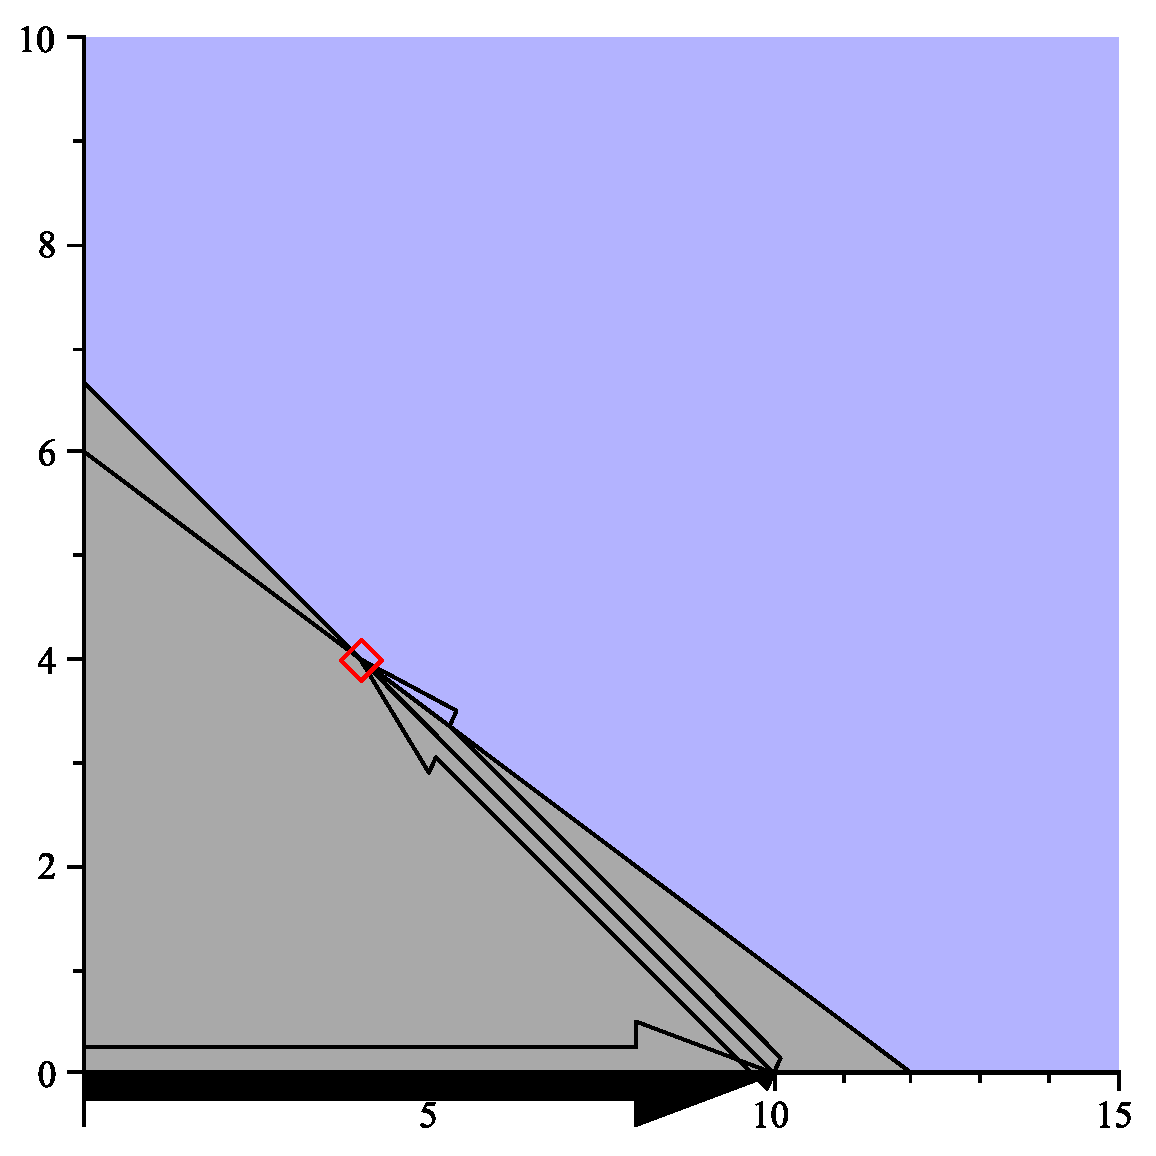
\includegraphics[scale=0.35]{PhaseISimplex.pdf}
\caption{Finding an initial feasible point: Artificial variables are introduced into the problem. These variables allow us to move through non-feasible space. Once we reach a feasible extreme point, the process of optimizing Problem $P_1$ stops.}
\label{fig:PhaseISimplex}
\end{figure}
\label{ex:ArtificialVariables}

We could now continue on to solve the initial problem we were given. At this point, our basic feasible solution makes $x_2$ and $x_1$ basic variables and $s_1$ and $s_2$ non-basic variables. Our problem data are:
\begin{displaymath}
\mathbf{x}_\mathbf{B} = \begin{bmatrix}x_2 \\ x_1\end{bmatrix}\quad
\mathbf{x}_\mathbf{N} = \begin{bmatrix}s_1 \\ s_2\end{bmatrix}
\end{displaymath}
Note that we keep the basic variables in the order in which we find them at the end of the solution to our first problem.  
\begin{displaymath}
\mathbf{A} = \begin{bmatrix}
1 & 2 & -1 & 0 \\
2 & 3 & 0 & -1
\end{bmatrix}\;\;\;\;
\mathbf{b} = \begin{bmatrix}
12\\20
\end{bmatrix}
\end{displaymath}
\begin{displaymath}
\mathbf{B} = \begin{bmatrix}
2 & 1\\
3 & 2
\end{bmatrix}\;\;\;\;
\mathbf{N} = \begin{bmatrix}
-1 & 0\\
 0 & -1
\end{bmatrix}\;\;\;\;
\mathbf{B}^{-1}\mathbf{b} = 
\begin{bmatrix}
4\\4
\end{bmatrix}
\end{displaymath}
\begin{displaymath}
\mathbf{c_B} = \begin{bmatrix}
2\\
1
\end{bmatrix}\;\;\;\;
\mathbf{c_N} = \begin{bmatrix}
0\\0
\end{bmatrix}
\end{displaymath}
\begin{displaymath}
\mathbf{c}_\mathbf{B}^TB^{-1}\mathbf{b} = 12\;\;\;\;
\mathbf{c}_\mathbf{B}^T\mathbf{B}^{-1}\mathbf{N} - \mathbf{c}_{\mathbf{N}}^T = \begin{bmatrix}
-1 & 0
\end{bmatrix}
\end{displaymath}

\textit{Notice that we don't have to do a lot of work to get this information out of the last tableau in Expression \ref{eqn:LastPhase1Tableau}.} The matrix $\mathbf{B}^{-1}$ is actually positioned in the columns below the artificial variables. This is because we started with an identity matrix in this position. As always, the remainder of the matrix holds $\mathbf{B}^{-1}\mathbf{N}$. Thus, we can read this final tableau as:

\begin{equation}
\begin{array}{c}
\\
z\\
x_{2}\\
x_{1}
\end{array}
\left[
\begin{array}{c|ccc|c}
z & \mathbf{x}_\mathbf{B} & \mathbf{s} & \mathbf{x}_a & \text{RHS}\\
\hline
1 & \mathbf{0} & \mathbf{0} & -\mathbf{e} & 0\\
\hline
\mathbf{0} & \mathbf{I}_2 & \mathbf{B}^{-1}\mathbf{N}  & \mathbf{B}^{-1} & \mathbf{B}^{-1}\mathbf{b}
\end{array}
\right]
\label{eqn:LastPhase1TableauX}
\end{equation}
In our case from Expression \ref{eqn:LastPhase1Tableau} we have:
\begin{equation}
\begin{array}{c}
\\
z\\
x_{2}\\
x_{1}
\end{array}
\left[
\begin{array}{c|cc|cc|cc|c}
z & x_1 & x_2 & s_1 & s_2 & x_{a_1} & x_{a_2} & \text{RHS}\\
\hline
1 & 0 & 0 & 0 & 0 & -1 & -1 & 0\\
\hline
0 & 0 & 1 & -2 & 1  & 2 & -1 & 4\\
0 & 1 & 0 & 3  & -2 & -3 & 2 & 4\\
\hline
- & \multicolumn{2}{c}{\mathbf{I}_2} & \multicolumn{2}{c}{\mathbf{B}^{-1}\mathbf{N}} & \multicolumn{2}{c}{\mathbf{B}^{-1}} & \mathbf{B}^{-1}\mathbf{b}
\end{array}
\right]
%\label{eqn:LastPhase1Tableau}
\end{equation}

We can use this information (and the reduced costs and objective function we computed) to start our tableau to solve the problem with which we began. Our next initial tableau will be:
\begin{equation}
\begin{array}{c}
\\
z\\
x_{2}\\
x_{1}
\end{array}
\left[
\begin{array}{c|cccc|c}
z & x_1 & x_2 & s_1 & s_2  & \text{RHS}\\
\hline
1 & 0 & 0 & -1 & 0 & 12\\
\hline
0 & 0 & 1 & -2 & 1  & 4\\
0 & 1 & 0 & 3  & -2 & 4
\end{array}
\right]
%\label{eqn:LastPhase1Tableau}
\end{equation}

Notice all we've done is removed the artificial variables from the problem and substituted the newly computed reduced costs for $s_1$ and $s_2$ ($-1$ and $0$) into Row 0 of the tableau. We've also put the correct objective function value ($12$) into Row 0 of the right hand side. We're now ready to solve the original problem. However, since this is a \textit{minimization problem} we can see we're already at a point of optimality. Notice that all reduced costs are either negative or zero, suggesting that entering any non-basic variable will at best keep the objective function value the same and at worst make the objective function worse. Thus we conclude that an optimal solution for our original problem is $x^*_1 = x^*_2 = 4$ and $s^*_1 = s^*_2 = 0$.
\end{example}

\begin{theorem} Let $\mathbf{x}^*,\mathbf{x_a}^*$ be an optimal feasible solution to problem $P_1$. Problem $P$ is feasible if and only if $\mathbf{x_a}^*=\mathbf{0}$.
\end{theorem}
\begin{proof} We have already proved in Lemma \ref{lem:PhaseILem} that if $\mathbf{x_a}^*=\mathbf{0}$, then $\mathbf{x}^*$ is a feasible solution to $P$ and thus $P$ is feasible. 

Conversely, suppose that $P$ is feasible. Then $P$ has at least one basic feasible solution because the feasible region of $P$ is a polyhedral set and we are assured by Lemma \ref{lem:FiniteExtremePoints} that this set has at least one extreme point. Now we can simply let $\mathbf{x_a}^* = \mathbf{0}$ and $\mathbf{x}$ be this basic feasible solution to problem $P$. Then this is clearly an optimal solution to problem $P_1$ because it forces the objective value to its lower bound (zero).
\end{proof}

\section{The Two-Phase Simplex Algorithm}
The two phase simplex algorithm applies the results from the previous section to develop an end-to-end algorithm for solving an arbitrary linear programming problem. 
\begin{algorithm}
\caption{Two-Phase Simplex Algorithm}
\label{alg:TwoPhaseSimplex}
\begin{center}
\begin{minipage}[t]{\textwidth-1em}
\underline{\textbf{Two-Phase Simplex Algorithm}}
\begin{enumerate*}
\item Given a problem of the form of the general maximization (or minimization) problem from Equation \ref{eqn:GeneralLPMax}, convert it to standard form:
\begin{displaymath}
P\left\{
\begin{aligned}
\max\;\; & \mathbf{c}^T\mathbf{x}\\
s.t.\;\; & \mathbf{A}\mathbf{x} = \mathbf{b}\\
& \mathbf{x} \geq \mathbf{0}
\end{aligned}\right.
\end{displaymath}
with $\mathbf{b} \geq \mathbf{0}$. 

\item Introduce auxiliary variables $\mathbf{x_a}$ and solve the \textbf{Phase I} problem:
\begin{displaymath}
P_1\left\{
\begin{aligned}
\min\;\; & \mathbf{e}^T\mathbf{x_a}\\
s.t.\;\; & \mathbf{A}\mathbf{x} + \mathbf{I}_m\mathbf{x_a} = \mathbf{b}\\
& \mathbf{x},\mathbf{x_a} \geq \mathbf{0}
\end{aligned}\right.
\end{displaymath}

\item If $\mathbf{x}_\mathbf{a}^* = \mathbf{0}$, then an initial feasible solution has been identified. This solution can be converted into a basic feasible solution as we discuss below. Otherwise, there is no solution to Problem $P$.

\item Use the Basic Feasible solution identified in Step 3 to start the Simplex Algorithm (compute the reduced costs given the $\mathbf{c}$ vector). 

\item Solve the \textbf{Phase II} problem:
\begin{displaymath}
P\left\{
\begin{aligned}
\max\;\; & \mathbf{c}^T\mathbf{x}\\
s.t.\;\; & \mathbf{A}\mathbf{x} = \mathbf{b}\\
& \mathbf{x} \geq \mathbf{0}
\end{aligned}\right.
\end{displaymath}
\end{enumerate*}
\end{minipage}
\end{center}
\end{algorithm}

When we solve the Phase I problem, if $\mathbf{x}_\mathbf{a}^* \neq \mathbf{0}$ at optimality, then there is no solution. If $\mathbf{x}_\mathbf{a}^* = \mathbf{0}$, then there are two possibilities: 
\begin{enumerate}
\item The basis consists only of variables in the vector $\mathbf{x}$; i.e., no auxiliary variable is in the basis.
\item There is some auxiliary variable $x_{a_i}=0$ and this variable is in the basis; i.e., the solution is degenerate and the degeneracy is expressed in an auxiliary variable.
\end{enumerate}

\subsection{Case I: $\mathbf{x}_\mathbf{a} = \mathbf{0}$ and is out of the basis}

If $\mathbf{x}_\mathbf{a} = \mathbf{0}$ and there are not elements of the vector $\mathbf{x}_\mathbf{a}$ in the basis, then we have identified a basic feasible solution $\mathbf{x} = [\mathbf{x}_\mathbf{B}\;\;\mathbf{x}_\mathbf{N}]^T$. Simply allow the non-zero basic elements (in $\mathbf{x}$) to be $\mathbf{x}_\mathbf{B}$ and the remainder of the elements (not in $\mathbf{x_a}$) are in $\mathbf{x}_\mathbf{N}$. We can then begin Phase II using this basic feasible solution.

\subsection{Case II: $\mathbf{x}_\mathbf{a} = \mathbf{0}$ and is not out of the basis}

If $\mathbf{x}_\mathbf{a} = \mathbf{0}$ and there is at least one artificial variable still in the basis, then we have identified a degenerate solution to the Phase I problem. Theoretically we could proceed directly to Phase II, assigning $0$ coefficients to the artificial variables as long as we ensure that \textit{no artificial variable ever becomes positive again}. \cite{BJS04} notes that this can be accomplished by selective pivoting, however it is often more efficient and simpler to remove the artificial variables completely from the basis before proceeding to Phase II. 

To remove the artificial variables from the basis, let us assume that we can arrange Rows $1 - m$ of the Phase I simplex tableau as follows:
\begin{equation}
\begin{array}{l|ccccc}
& \mathbf{x}_\mathbf{B} & \mathbf{x_{B_a}} & \mathbf{x_N} & \mathbf{x_{N_a}} & \text{RHS}\\
\hline
\mathbf{x_B} & \mathbf{I}_k & \mathbf{0} & \mathbf{R}_1 & \mathbf{R}_3 & \overline{\mathbf{b}}\\
\mathbf{x_{B_a}} & \mathbf{0} & \mathbf{I}_{m-k} & \mathbf{R}_2 & \mathbf{R}_4 & \mathbf{0}
\end{array}
\label{eqn:PhaseITableau}
\end{equation}
Column swapping ensures we can do this, if we so desire. Our objective is to replace elements in $\mathbf{x_{B_a}}$ (the basic artificial variables) with elements from $\mathbf{x_N}$ non-basic, non-artificial variables. Thus, we will attempt to pivot on elements in the matrix $\mathbf{R}_2$. Clearly since the Phase I coefficients of the variables in $\mathbf{x_N}$ are zero, pivoting in these elements will not negatively impact the Phase I objective value. Thus, if the element in position $(1,1)$ is non-zero, then we can enter the variable $x_{N_1}$ into the basis and remove the variable $x_{B_{a_1}}$. This will produce a new tableau with structure similar to the one given in Equation \ref{eqn:PhaseITableau} except there will be $k+1$ non-artificial basic variables and $m-k-1$ artificial basic variables. Clearly if the element in position $(1,1)$ in matrix $\mathbf{R}_2$ is zero, then we must move to a different element for pivoting. 

In executing the procedure discussed above, one of two things will occur: 
\begin{enumerate}
\item The matrix $\mathbf{R}_2$ will be transformed into $\mathbf{I}_{m-k}$ or
\item A point will be reached where there are no longer any variables in $\mathbf{x_N}$ that can be entered into the basis because all the elements of $\mathbf{R}_2$ are zero.
\end{enumerate}

In the first case, we have removed all the artificial variables from the basis in Phase I and we can proceed to Phase II with the current basic feasible solution. In the second case, we will have shown that:
\begin{equation}
\mathbf{A} \sim 
\left[
\begin{array}{cc}
\mathbf{I}_k & \mathbf{R_1}\\
\mathbf{0} & \mathbf{0}
\end{array}\right]
\end{equation}
This shows that the $m-k$ rows of $\mathbf{A}$ are \textit{not} linearly independent of the first $k$ rows and thus the matrix $\mathbf{A}$ did not have full row rank. When this occurs, we can discard the last $m-k$ rows of $\mathbf{A}$ and simply proceed with the solution given in $\mathbf{x}_\mathbf{B} = \overline{\mathbf{b}}$, $\mathbf{x}_\mathbf{N} = \mathbf{0}$. This is a basic feasible solution to the new matrix $\mathbf{A}$ in which we have removed the redundant rows.

\begin{example} Once execution of the Phase I simplex algorithm is complete, the reduced costs of the current basic feasible solution must be computed. These can be computed during Phase I by adding an additional ``$z$'' row to the tableau. In this case, the initial tableau has the form:
\begin{equation}
\begin{array}{c}
\\
z_{II}\\
z\\
x_{a_1}\\
x_{a_2}
\end{array}
\left[
\begin{array}{c|cccccc|c}
z & x_1 & x_2 & s_1 & s_2 & x_{a_1} & x_{a_2} & \text{RHS}\\
\hline
1 & -1 & -2 & 0 & 0 & 0 & 0 & 0\\
\hline
1 & 3 & 5 & -1 & -1 & 0 & 0 & 32\\
\hline
0 & 1 & 2 & -1 & 0  & 1 & 0 & 12\\
0 & 2 & 3 & 0  & -1 & 0 & 1 & 20
\end{array}
\right]
\end{equation}
The first row ($z_{II}$) is computed for the objective function:
\begin{equation}
x_1 + 2x_2 + 0s_1 + 0s_2 + 0x_{a_1} + 0x_{a_2},
\end{equation}
which is precisely the Phase II problem, except we never allow the artificial variables $x_{a_1}$ and $x_{a_2}$ to carry into the Phase II problem. If we carry out the same steps we did in Example \ref{ex:ArtificialVariables} then we obtain the sequence of tableaux:\\
\noindent\textbf{TABLEAU I}
\begin{displaymath}
\begin{array}{c}
\\
z_{II}\\
z\\
x_{a_1}\\
x_{a_2}
\end{array}
\left[
\begin{array}{c|cccccc|c}
z & x_1 & x_2 & s_1 & s_2 & x_{a_1} & x_{a_2} & \text{RHS}\\
\hline
1 & -1 & -2 & 0 & 0 & 0 & 0 & 0\\
\hline
1 & 3 & 5 & -1 & -1 & 0 & 0 & 32\\
\hline
0 & 1 & 2 & -1 & 0  & 1 & 0 & 12\\
0 & \fbox{2} & 3 & 0  & -1 & 0 & 1 & 20
\end{array}
\right]
\begin{array}{c}
\text{MRT}(x_1)\\
\hline
\\
\\
12\\
20/2 = 10
\end{array}
\end{displaymath}
\noindent\textbf{TABLEAU II}
\begin{displaymath}
\begin{array}{c}
\\
z_{II}\\
z\\
x_{a_1}\\
x_{1}
\end{array}
\left[
\begin{array}{c|cccccc|c}
z & x_1 & x_2 & s_1 & s_2 & x_{a_1} & x_{a_2} & \text{RHS}\\
\hline
1 & 0 & -1/2 & 0 & -1/2 & 0 & 1/2 & 10\\
\hline
1 & 0 & 1/2 & -1 & 1/2 & 0 & -3/2 & 2\\
\hline
0 & 0 & \fbox{1/2} & -1 & 1/2  & 1 & -1/2 & 2\\
0 & 1 & 3/2 & 0  & -1/2 & 0 & 1/2 & 10
\end{array}
\right]
\begin{array}{c}
\text{MRT}(x_1)\\
\hline
\\
\\
4\\
20/3
\end{array}
\end{displaymath}
\noindent\textbf{TABLEAU III}
\begin{displaymath}
\begin{array}{c}
\\
z_{II}\\
z\\
x_{2}\\
x_{1}
\end{array}
\left[
\begin{array}{c|cccccc|c}
z & x_1 & x_2 & s_1 & s_2 & x_{a_1} & x_{a_2} & \text{RHS}\\
\hline
1 & 0 & 0 & -1 & 0 & 1 & 0 & 12\\
\hline
1 & 0 & 0 & 0 & 0 & -1 & -1 & 0\\
\hline
0 & 0 & 1 & -2 & 1  & 2 & -1 & 4\\
0 & 1 & 0 & 3  & -2 & -3 & 2 & 4
\end{array}
\right]
\end{displaymath}
We again arrive at the end of Phase I, but we are now prepared to immediately execute Phase II with the tableau:
\begin{displaymath}
\begin{array}{c}
\\
z_{II}\\
x_{2}\\
x_{1}
\end{array}
\left[
\begin{array}{c|cccc|c}
z & x_1 & x_2 & s_1 & s_2 & \text{RHS}\\
\hline
1 & 0 & 0 & -1 & 0 &  12\\
\hline
0 & 0 & 1 & -2 & 1  &  4\\
0 & 1 & 0 & 3  & -2 &  4
\end{array}
\right]
\end{displaymath}
In this case, we see that we are already at an optimal solution for a minimization problem because the reduced costs are all less than or equal to zero. We also note that since the reduced cost of the non-basic variable $s_2$ is zero, there are alternative optimal solutions. 
\label{ex:TwoPhase}
\end{example}

\section{The Big-M Method} 
The Big-M method is similar to the two-phase simplex algorithm, except that it essentially attempts to execute Phase I and Phase II in a single execution of the simplex algorithm. 

In the Big-M method we modify problem $P$ with artificial variables as we did in the two-phase simplex method but we also modify the objective function:
\begin{equation}
P_M\left\{
\begin{aligned}
\max\;\; & \mathbf{c}^T\mathbf{x} - M\mathbf{e}^T\mathbf{x_a}\\
s.t.\;\; & \mathbf{A}\mathbf{x} + \mathbf{I}_m\mathbf{x_a} = \mathbf{b}\\
& \mathbf{x}, \mathbf{x_a} \geq \mathbf{0}
\end{aligned}\right.
\label{eqn:BigM}
\end{equation}
Here, $M$ is a large positive constant, much larger than the largest coefficient in the vector $\mathbf{c}$. The value of $M$ is usually chosen to be at least 100 times larger than the largest coefficient in the original objective function.

\begin{remark} In the case of a minimization problem, the objective function in the Big-M method becomes:
\begin{equation}
\min\;\;\mathbf{c}^T\mathbf{x} + M\mathbf{e}^T\mathbf{x_a}
\label{eqn:MinObjBigM}
\end{equation}
\end{remark}

\begin{exercise}
In Exercise \ref{exer:MinForMax} we showed that every maximization problem can be written as a minimization problem (and vice-versa). Show that Equation \ref{eqn:MinObjBigM} follows by changing Problem $P_M$ into a minimization problem.
\end{exercise}

\begin{lemma} Suppose that problem $P_M$ is unbounded. If problem $P$ is feasible, then it is unbounded.
\label{lem:UnboundedBigM}
\end{lemma}
\begin{proof} If $P_M$ is unbounded, then there is some direction direction:
\begin{displaymath}
\mathbf{d}_M = \begin{bmatrix}\mathbf{d}\\\mathbf{d_a}\end{bmatrix}
\end{displaymath} 
to the feasible region of Problem $P_M$. Furthermore, $\mathbf{d}\geq \mathbf{0}$ and $\mathbf{d_a} \geq \mathbf{0}$ and as a whole $\mathbf{d}_M \neq \mathbf{0}$. For this problem to be unbounded, it suffices that:
\begin{equation}
\mathbf{c}^T\mathbf{d} - M\mathbf{e}^T\mathbf{d}_a > 0
\label{eqn:BigMDir}
\end{equation}
by Corollary \ref{cor:OptimalityDirections}. 

Since we are free to choose $M$ as large as we like, it follows that for a large value of $M$, the left-hand-side of Inequality \ref{eqn:BigMDir} must be negative \textit{unless} 
$\mathbf{d_a} = \mathbf{0}$. 

The fact that $\mathbf{d}_M$ is a direction implies that $\mathbf{A}\mathbf{d} + \mathbf{I}_m\mathbf{d_a} = \mathbf{0}$ and therefore $\mathbf{A}\mathbf{d} = \mathbf{0}$. 
We know further that $\mathbf{d} \geq \mathbf{0}$ and $\mathbf{d} \neq \mathbf{0}$. Thus it follows that we have identified a direction $\mathbf{d}$ of the feasible region for Problem $P$. Furthermore, we know that following this direction must result in an unbounded objective function for $P$ since the coefficients of the artificial variables are all negative.
\end{proof}

\begin{remark} Lemma \ref{lem:UnboundedBigM} tells us that if the Problem $P_M$ is unbounded, then we know that there is no \textit{useful} solution to Problem $P$. If Problem $P$ has non-empty feasible region, then it [Problem $P$] is unbounded and thus there is no useful solution. On the other hand, if Problem $P$ has no feasible solution, there is still no useful solution to Problem $P$. \textit{In either case}, we may need to re-model the problem to obtain a useful result.
\end{remark}

\begin{theorem} If Problem $P$ is feasible and has a finite solution. Then there is an $M > 0$ so that the optimal solution to $P_M$ has all artificial variables non-basic and thus the solution to Problem $P$ can be extracted from the solution to Problem $P_M$.
\end{theorem}
\begin{proof} By contrapositive applied to Lemma \ref{lem:UnboundedBigM} we know that Problem $P_M$ is bounded. By the Cartheodory Characterization theorem, we may enumerate the extreme points of the feasible region of Problem $P_M$: call these $\mathbf{y}_1,\dots,\mathbf{y}_k$ where:
\begin{displaymath}
\mathbf{y} = \begin{bmatrix}
\mathbf{x}\\\mathbf{x_a}
\end{bmatrix}
\end{displaymath}
Let $z_{M_1},\dots z_{M_k}$ be the objective function value of Problem $P_M$ at each of these extreme points. Since $P$ is feasible, at least one of these extreme points has $\mathbf{x_a} = \mathbf{0}$. Let us sub-divide the extreme points in $\mathcal{Y}_a = \{\mathbf{y}_1,\dots,\mathbf{y}_l\}$ and $\mathcal{Y}=\{\mathbf{y}_{l+1}, \dots, \mathbf{y}_k\}$ where the points in $\mathcal{Y}_a$ are the extreme points such that there is at least one non-zero artificial variable and the points in $\mathcal{Y}$ are the extreme points where all artificial variables are zero. At any extreme point in $\mathcal{Y}$ we know that \textit{at most} $m$ elements of the vector $\mathbf{x}$ are non-zero and therefore, every extreme point in $\mathcal{Y}$ corresponds to an extreme point of the original problem $P$. Since Problem $P$ has a finite solution, it follows that the optimal solution to problem $P$ occurs at some point in $\mathcal{Y}$, by Theorem \ref{thm:EPSoln}. Furthermore the value of the objective function for Problem $P$ is precisely the same as the value of the objective function of Problem $P_M$ for each point in $\mathcal{Y}$ because $\mathbf{x_a} = \mathbf{0}$. Define:
\begin{equation}
z^\text{min}_P = \min_{\mathbf{y} \in \mathcal{Y}} \{\mathbf{c}^T\mathbf{x} : \mathbf{y} = [\mathbf{x} \;\; \mathbf{x_a}]^T\}
\end{equation}

At each extreme point in $\mathcal{Y}_a$, the value of the objective function of Problem $P_M$ is a function of the value of $M$, which we are free to choose. Therefore, choose $M$ so that:
\begin{equation}
\max_{\mathbf{y} \in \mathcal{Y}_a} \{\mathbf{c}^T\mathbf{x} - M\mathbf{e}^T\mathbf{x_a}: \mathbf{y} = [\mathbf{x} \;\; \mathbf{x_a}]^T\} < z^\text{min}_P
\end{equation}
Such a value exists for $M$ since there are only a finite number of extreme points in $\mathcal{Y}$. Our choice of $M$ ensures that the optimal solution to $P_M$ occurs at an extreme point where $\mathbf{x_a} = \mathbf{0}$ and the $\mathbf{x}$ component of $\mathbf{y}$ is the solution to Problem $P$. 
\end{proof}

\begin{remark}
Another way to look at the proof of this theorem is to think of defining $M$ in such a way so that at any extreme point where $\mathbf{x_a} \neq \mathbf{0}$, the objective function can always be made larger by moving to any extreme point that is feasible to Problem $P$. Thus the simplex algorithm will move among the extreme points seeking to leave those that are not feasible to Problem $P$ because they are less desirable.
\end{remark}

\begin{theorem} Suppose Problem $P$ is infeasible. Then there is no value of $M$ that will drive the all the artificial variables from the basis of Problem $P_M$. 
\end{theorem}
\begin{proof} If such an $M$ existed, then $\mathbf{x_a} = \mathbf{0}$ and the resulting values of $\mathbf{x}$ represents a feasible solution to Problem $P$, which contradicts our assumption that Problem $P$ was infeasible.
\end{proof}

\begin{remark} The Big-M method is not particularly effective for solving real-world problems. The introduction of a set of variables with large coefficients ($M$) can lead to round-off errors in the execution of the simplex algorithm. (Remember, computers can only manipulate numbers in binary, which means that all floating point numbers are restricted in their precision to the machine precision of the underlying system OS. This is generally given in terms of the largest amount of memory that can be addressed in bits. This has led, in recent times, to operating system manufacturers selling their OS's as ``32 bit'' or ``64 bit.'' When solving real-world problems, these issue can become a real factor with which to contend.

Another issue is we have no way of telling how large $M$ should be without knowing that Problem $P$ is feasible, which is precisely what we want the Big-M method to tell us! The general rule of thumb provided earlier will suffice. 
\end{remark}

\begin{example} 
Suppose we solve the problem from Example \ref{ex:ArtificialVariables} using the Big-M method. Our problem is:
\begin{equation}
\begin{aligned}
\min\;\; & 	x_1 + 2x_2\\
s.t.\;\; &	x_1 + 2x_2 \geq 12\\
		 &	2x_1 + 3x_2 \geq 20\\
		 &	x_1, x_2 \geq 0
\end{aligned}
\end{equation}
Again, this problem has standard form:
\begin{equation}
\begin{aligned}
\min\;\; & 	x_1 + 2x_2\\
s.t.\;\; &	x_1 + 2x_2 - s_1  = 12\\
		 &	2x_1 + 3x_2 - s_2 = 20\\
		 &	x_1, x_2, s_1, s_2 \geq 0
\end{aligned}
\end{equation}

To execute the Big-M method, we'll choose $M = 300$ which is larger than 100 times the largest coefficient of the objective function of the original problem. Our new problem becomes:
\begin{equation}
\begin{aligned}
\min\;\; & 	x_1 + 2x_2 + 300x_{a_1} + 300x_{a_2}\\
s.t.\;\; &	x_1 + 2x_2 - s_1  + x_{a_1} = 12\\
		 &	2x_1 + 3x_2 - s_2  + x_{a_2}= 20\\
		 &	x_1, x_2, s_1, s_2,x_{a_1},x_{a_2} \geq 0
\end{aligned}
\end{equation}
Since this is a \textit{minimization} problem, we \textit{add} $M\mathbf{e}^T\mathbf{x_a}$ to the objective function. Letting $x_{a_1}$ and $x_{a_2}$ be our initial basis, we have the series of tableaux:\\
\noindent\textbf{TABLEAU I}
\begin{displaymath}
\begin{array}{c}
\\
z\\
x_{a_1}\\
x_{a_2}
\end{array}
\left[
\begin{array}{c|cccccc|c}
z & x_1 & x_2 & s_1 & s_2 & x_{a_1} & x_{a_2} & \text{RHS}\\
\hline
1 & 899 & 1498 & -300 & -300 & 0 & 0 & 9600\\
\hline
0 & 1 & 2 & -1 & 0  & 1 & 0 & 12\\
0 & \fbox{2} & 3 & 0  & -1 & 0 & 1 & 20
\end{array}
\right]
\begin{array}{c}
\text{MRT}(x_1)\\
\hline
\\
12\\
20/2 = 10
\end{array}
\end{displaymath}
\noindent\textbf{TABLEAU II}
\begin{displaymath}
\begin{array}{c}
\\
z\\
x_{a_1}\\
x_{1}
\end{array}
\left[
\begin{array}{c|cccccc|c}
z & x_1 & x_2 & s_1 & s_2 & x_{a_1} & x_{a_2} & \text{RHS}\\
\hline
1 & 0 & 299/2 & -300 & 299/2 & 0 & -899/2 & 610\\
\hline
0 & 0 & \fbox{1/2} & -1 & 1/2  & 1 & -1/2 & 2\\
0 & 1 & 3/2 & 0  & -1/2 & 0 & 1/2 & 10
\end{array}
\right]
\begin{array}{c}
\text{MRT}(x_1)\\
\hline
\\
4\\
20/3
\end{array}
\end{displaymath}
\noindent\textbf{TABLEAU III}
\begin{displaymath}
\begin{array}{c}
\\
z\\
x_{2}\\
x_{1}
\end{array}
\left[
\begin{array}{c|cccccc|c}
z & x_1 & x_2 & s_1 & s_2 & x_{a_1} & x_{a_2} & \text{RHS}\\
\hline
1 & 0 & 0 & -1 & 0 & -299 & -300 & 12\\
\hline
0 & 0 & 1 & -2 & 1  & 2 & -1 & 4\\
0 & 1 & 0 & 3  & -2 & -3 & 2 & 4
\end{array}
\right]
\end{displaymath}
It is worth noting that this is essentially the same series of tableau we had when executing the Two-Phase method, but we have to deal with the large $M$ coefficients in our arithmetic.
\end{example}

\section{The Single Artificial Variable Technique}
Consider the system of equations $\mathbf{A}\mathbf{x} = \mathbf{b}$ that composes a portion of the feasible region of Problem $P$. Suppose we chose some sub-matrix of $\mathbf{A}$ to be our basis matrix $\mathbf{B}$ irrespective of whether the solution $\mathbf{x}_\mathbf{B} = \mathbf{B}^{-1}\mathbf{b} \geq \mathbf{0}$. If $\mathbf{A}$ has full row rank, then clearly such a matrix exists. The resulting basic solution with basis $\mathbf{B}$ is called a \textit{crash basis}. 

If $\overline{\mathbf{b}} = \mathbf{B}^{-1}\mathbf{b}  \geq \mathbf{0}$, then we have (by luck) identified an initial basic feasible solution and we can proceed directly to execute the simplex algorithm as we did in Chapter 5. Suppose that $\overline{\mathbf{b}} \not\geq \mathbf{0}$. Then we can form the new system:
\begin{equation}
\mathbf{I}_m\mathbf{x}_\mathbf{B} + \mathbf{B}^{-1}\mathbf{N} + \mathbf{y}_ax_a = \overline{\mathbf{b}}
\end{equation}
where $x_a$ is a single artificial variable and $\mathbf{y}_a$ is a (row) vector of coefficients for $x_a$ so that:
\begin{equation}
\mathbf{y}_{a_i} = \begin{cases}
-1 & \text{if $\overline{\mathbf{b}}_i < 0$}\\
0 & \text{else}
\end{cases}
\end{equation}
\begin{lemma} Suppose we enter $x_a$ into the basis by pivoting on the row of the simplex tableau with most negative right hand side. That is, $x_a$ is exchanged with variable $\mathbf{x}_{\mathbf{B}_j}$ having most negative value. Then the resulting solution is a basic feasible solution to the constraints:
\begin{equation}
\begin{aligned}
&\mathbf{I}_m\mathbf{x}_\mathbf{B} + \mathbf{B}^{-1}\mathbf{N} + \mathbf{y}_ax_a = \overline{\mathbf{b}}\\
&\mathbf{x}, x_a \geq \mathbf{0}
\end{aligned}
\end{equation}
\label{lem:SingleArtificialVar}
\end{lemma}
\begin{exercise} Prove Lemma \ref{lem:SingleArtificialVar}.
\end{exercise}
The resulting basic feasible solution can either be used as a starting solution for the two-phase simplex algorithm with the single artificial variable \textit{or} the Big-M method. For the two-phase method, we would solve the Phase I problem:
\begin{equation}
\begin{aligned}
\min\;\; & x_a\\
s.t.\;\; & \mathbf{A}\mathbf{x} + \mathbf{B}_0\mathbf{y}_a x_a = \mathbf{b}\\
&\mathbf{x},x_a \geq \mathbf{0}
\end{aligned}
\label{eqn:SingleVarPhaseI}
\end{equation}
where $\mathbf{B}_0$ is the initial crash basis we used to identify the coefficients of single artificial variable. Equation \ref{eqn:SingleVarPhaseI} is generated by multiplying by $\mathbf{B}_0$ on both sides of the inequalities.

\begin{example}
Suppose we were interested in the constraint set:
\begin{equation}
\begin{aligned}
&	x_1 + 2x_2 - s_1  = 12\\
&	2x_1 + 3x_2 - s_2 = 20\\
&	x_1, x_2, s_1, s_2 \geq 0
\end{aligned}
\end{equation}
We can choose the crash basis:
\begin{equation}
\begin{bmatrix}
-1 & 0\\
0 & -1
\end{bmatrix}
\end{equation}
corresponding to the variables $s_1$ and $s_2$. Then we obtain the system:
\begin{equation}
\begin{aligned}
&	-x_1  - 2x_2 + s_1  = -12\\
&	-2x_1 - 3x_2 + s_2 = -20\\
\end{aligned}
\end{equation}
That is, $s_1 = -12$ and $s_2 = -20$ is our basic solution, which is not feasible. We append the artificial variable with coefficient vector $\mathbf{y}_a = [-1\;\;-1]^T$ (since both elements of the right-hand-side are negative) to obtain:
\begin{equation}
\begin{aligned}
&	-x_1  - 2x_2 + s_1 -x_a = -12\\
&	-2x_1 - 3x_2 + s_2 -x_a = -20\\
\end{aligned}
\end{equation}
If we build a tableau for Phase I with this current BFS, we obtain:
\begin{displaymath}
\begin{array}{c}
\\
z\\
s_{1}\\
s_{2}
\end{array}
\left[
\begin{array}{c|ccccc|c}
z & x_1 & x_2 & s_1 & s_2 & x_{a} & \text{RHS}\\
\hline
1 & 0 & 0 & 0 & 0 & -1& 0\\
\hline
0 & -1 & -2 & 1 & 0  & -1 &  -12\\
0 & -2 & -3 & 0 & 1  & -1 & -20
\end{array}
\right]
\end{displaymath}
We enter the variable $x_a$ and pivot out variable $s_2$ which has the \textbf{most negative} right hand side to obtain the initial feasible tableau:
\begin{displaymath}
\begin{array}{c}
\\
z\\
s_{1}\\
x_a
\end{array}
\left[
\begin{array}{c|ccccc|c}
z & x_1 & x_2 & s_1 & s_2 & x_{a} & \text{RHS}\\
\hline
1 & 2 & 3 & 0 & 1 & 0& 20\\
\hline
0 & 1 & 1 & 1 & -1  & 0 &  8\\
0 & 2 & 3 & 0 & -1  & 1  & 20
\end{array}
\right]
\end{displaymath}
We can now complete the Phase I process and execute the simplex algorithm until we drive $x_a$ from the basis and reduce the right-hand-side to $0$. At this point we will have identified an initial basic feasible solution to the initial problem and we can execute Phase II.
\end{example}

\begin{remark} Empirical evidence suggests that the single artificial variable technique is not as efficient as the two-phase or Big-M method. Thus, it is presented as an historical component of the development of efficient implementations of the Simplex algorithm and not as a realistic technique for implementation in production systems.
\end{remark}

\section{Problems that Can't be Initialized by Hand}
In these notes, we have so far considered very small problems that could easily be solved graphically. Determining an initial basic feasible solution requires little more than trial and error. These problems hardly require the use of Phase I methods. 

To provide an example of a class of problems that can easily generate large numbers of variables, we will consider a multi-period inventory control problem. These problems can easily generate large numbers of variables and constraints, even in small problems.

\begin{example} McLearey's Shamrock Emporium produces and sells shamrocks for three days each year: the day before St. Patrick's Day, St. Patrick's Day and the day after St. Patrick's day. This year, McLearey had 10 shamrocks left over from last year's sale. This year, he expects to sell 100 shamrocks the day before St. Patrick's Day, 200 shamrocks the day of St. Patrick's day and 50 shamrocks the day after St. Patrick's day. 

It costs McLearey \$2 to produce each Shamrock and \$0.01 to store a Shamrock over night. Additionally, McLearey can put shamrocks into long term storage for \$0.05 per shamrock.

McLearey can produce at most 150 shamrocks per day. Shamrocks must be produced within two days of being sold (or put into long term storage) otherwise, they wilt. Assuming that McLearey must meet his daily demand and will not start producing Shamrocks early, he wants to know how many shamrocks he should make and store on each day to minimize his cost.

To determine an answer to this problem, note that we have time as a parameter: time runs over three days. Let $x_t$ be the number of shamrocks McLearey makes on day $t$ ($t=1,2,3$) and let $y_t$ be the number of shamrocks McLearey stores on day $t$. There is also a parameter $y_0 = 10$, the number of shamrocks left over from last year. 

McLearey's total cost (in cents) can the be written as:
\begin{equation}
z = 200x_1 + 200x_2 + 200x_3 + y_1 + y_2 + 5y_3
\end{equation} 
Additionally, there are some constraints linking production, storage and demand. These constraints are depicted graphically in Figure \ref{fig:Shamrock}. Multiperiod inventory models operate on a principle of conservation of flow. Manufactured goods and previous period inventories flow into the box representing each period. Demand and next period inventories flow out of the box representing each period. This inflow and outflow must be equal to account for all shamrocks produced. This is depicted below:
\begin{figure}[htbp]
\centering
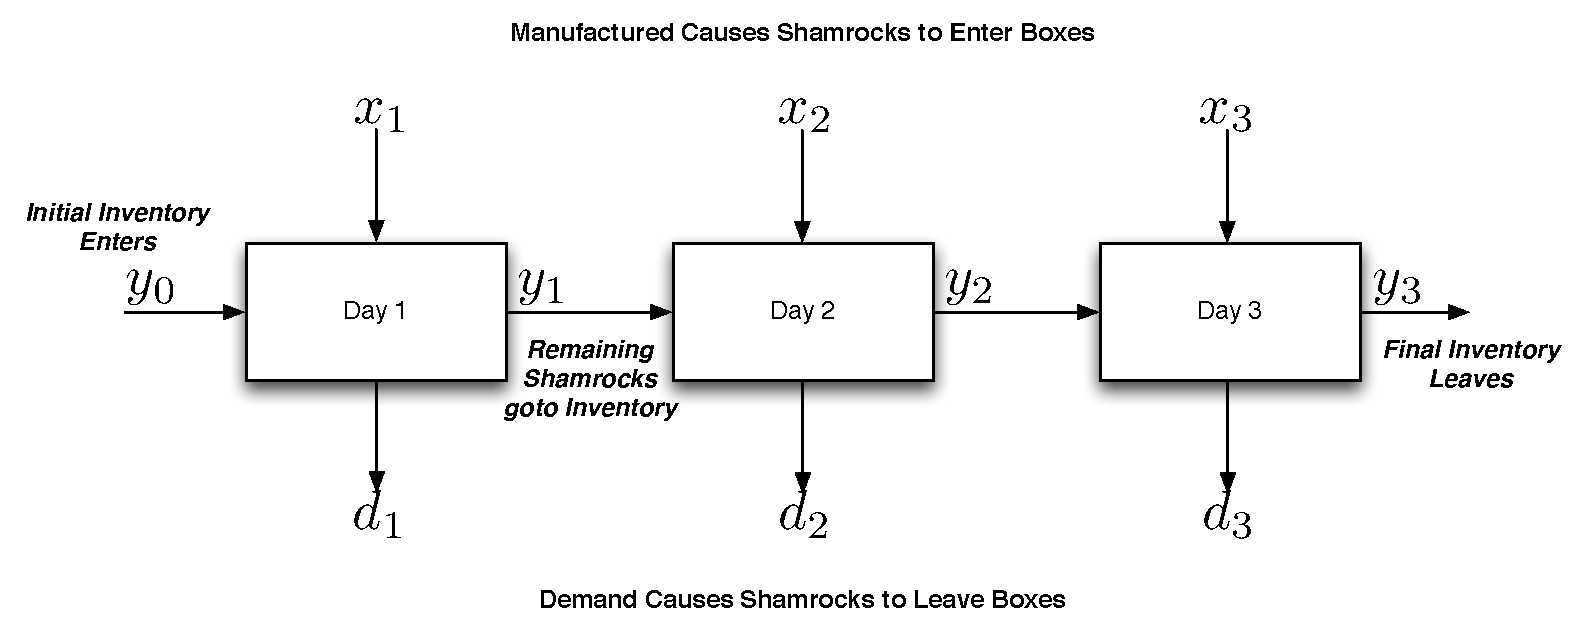
\includegraphics[scale=0.35]{ShamrockFigure.pdf}
\caption{Multiperiod inventory models operate on a principle of conservation of flow. Manufactured goods and previous period inventories flow into the box representing each period. Demand and next period inventories flow out of the box representing each period. This inflow and outflow must be equal to account for all production.}
\label{fig:Shamrock}
\end{figure}

This means that:
\begin{equation}
y_{t-1} + x_t = y_{t} + d_t\quad\forall t
\end{equation}
This equation says that at period $t$ the amount of inventory carried over from period $t-1$ plus amount of shamrocks produced in period $t$ must be equal to the total demand in period $t$ plus any left over shamrocks at the end of period $t$. Clearly we also know that $x_t \geq 0$ for all $t$, since you cannot make a negative number of shamrocks. However, by also requiring $y_t \geq 0$ for all $t$, then we assert that our inventory can never be negative. A \textit{negative inventory} is a \textit{backorder}. Thus by saying that $y_t \geq 0$ we are also satisfying the requirement that McLearey satisfy his demand in each period. Note, when $t = 1$, then $y_{t-1} = y_0$, which is the parameter we defined above.

The complete problem describing McLearey's situation is:
\begin{equation}
\left\{
\begin{aligned}
\min\;\;&200x_1 + 200x_2 + 200x_3 + y_1 + y_2 + 5y_3\\
s.t.\;\;&y_{t-1} + x_t = y_{t} + d_t\quad\forall t \in \{1,2,3\}\\
&x_t \leq 150\quad\forall t \in \{1,2,3\}\\
&x_t,y_t \geq 0\quad\forall t \in \{1,2,3\}
\end{aligned}\right.
\end{equation}
Constraints of the form $x_t \leq 150$ for all $t$ come from the fact that McLearey can produce at most 150 shamrocks per day.

This simple problem now has 6 variables and 6 constraints plus 6 non-negativity constraints and it is non-trivial to determine a good initial basic feasible solution, especially since the problem contains both equality and inequality constraints. 

A problem like this can be solved in Matlab (see Chapter \ref{chap:Matrices}.\ref{sec:Matlab}), or on a commercial or open source solver like the GNU Linear Programming Kit (GLPK, \url{http://www.gnu.org/software/glpk/}). In Figure \ref{fig:GLPKModel} we show an example \textit{model file} that describes the problem. In Figure \ref{fig:GLPKData}, we show the data section of the GLPK model file describing McLearey's problem. Finally, figure \ref{fig:GLPKOutput} shows a portion of the output generated by the GLPK solver \texttt{glpsol} using this model. Note that there is no inventory in Year 3 (because it is too expensive) even though it might be beneficial to McLearey to hold inventory for next year. This is because the problem has no information about any other time periods and so, in a sense, the \textit{end of the world} occurs immediately after period 3. This type of \textit{end of the world} phenomenon is common in multi-period problems.
\begin{figure}[htbp]
\scriptsize
\verbatiminput{Shamrock.mod}
\caption{Input model to GLPK describing McLearey's Problem}
\label{fig:GLPKModel}
\normalsize
\end{figure}

\begin{figure}[htbp]
\scriptsize
\verbatiminput{Shamrock.dat}
\caption{Input data to GLPK describing McLearey's Problem}
\label{fig:GLPKData}
\normalsize
\end{figure}

\begin{figure}[htbp]
\scriptsize
\verbatiminput{ShamrockOut.txt}
\caption{Output from \texttt{glpsol} on the McLearey Problem.}
\label{fig:GLPKOutput}
\normalsize
\end{figure}
\end{example}

\chapter{Degeneracy and Convergence}
In this section, we will consider the problem of degeneracy and prove (at last) that there is an implementation of the Simplex Algorithm that is guaranteed to converge to an optimal solution, assuming one exists.

\section{Degeneracy Revisited}
We've already discussed degeneracy. Recall the following theorem from Chapter 5 that defines degeneracy in terms of the simplex tableau:

\vspace*{1em}
\noindent\textbf{Theorem \ref{thm:DegeneracyDef}.} \textit{Consider Problem $P$ (our linear programming problem). Let $\mathbf{B} \in \mathbb{R}^{m\times m}$ be a basis matrix corresponding to some set of basic variables $\mathbf{x_B}$. Let $\overline{\mathbf{b}} = \mathbf{B}^{-1}\mathbf{b}$. If $\overline{\mathbf{b}}_j = \mathbf{0}$ for some $j=1,\dots,m$, then $\mathbf{x}_B = \overline{\mathbf{b}}$ and $\mathbf{x_N} = \mathbf{0}$ is a degenerate extreme point of the feasible region of Problem $P$.}
\vspace*{1em}

We have seen in Example \ref{ex:ToyMakerDegenSimplex} that degeneracy can cause us to take extra steps on our way from an initial basic feasible solution to an optimal solution. When the simplex algorithm takes extra steps while remaining at the same degenerate extreme point, this is called \textit{stalling}. The problem can become much worse; for certain entering variable rules, the simplex algorithm can become locked in a cycle of pivots each one moving from one characterization of a degenerate extreme point to the next. The following example from Beale and illustrated in Chapter 4 of \cite{BJS04} demonstrates the point.

\begin{example} Consider the following linear programming problem:
\begin{equation}
\begin{aligned}
\min\;\;&-\frac{3}{4}x_4 + 20x_5 -\frac{1}{2}x_6 + 6x_7\\
s.t\;\;&x_1 + \frac{1}{4}x_4 - 8x_5 - x_6 + 9x_7 = 0\\
& x_2 + \frac{1}{2}x_4 - 12x_5 -\frac{1}{2}x_6 + 3x_7 = 0\\
&x_3 + x_6 = 1\\
&x_i \geq 0\;\;i=1,\dots,7
\end{aligned}
\end{equation}
It is conducive to analyze the $\mathbf{A}$ matrix of the constraints of this problem. We have:
\begin{equation}
\mathbf{A} = \begin{bmatrix}
1 & 0 & 0 & 1/4 & -8  & -1   & 9\\
0 & 1 & 0 & 1/2 & -12 & -1/2 & 3\\
0 & 0 & 1 & 0   &  0  & 1    & 0
\end{bmatrix}
\end{equation}
The fact that the $\mathbf{A}$ matrix contains an identity matrix embedded within it suggests that an initial basic feasible solution with basic variables $x_1$, $x_2$ and $x_3$ would be a good choice. This leads to a vector of reduced costs given by:
\begin{equation}
\mathbf{c_B}^T\mathbf{B}^{-1}\mathbf{N}-\mathbf{c_N}^T = 
\begin{bmatrix}3/4 & -20 & 1/2 & -6 \end{bmatrix}
\end{equation}
These yield an initial tableau with structure:
\begin{displaymath}
\begin{array}{c}
\\z\\x_1\\x_2\\x_3
\end{array}\left[
\begin{array}{c|ccccccc|c}
z & x_1 & x_2 & x_3 & x_4 & x_5 & x_6 & x_7 & RHS\\
\hline
1 & 0 & 0 & 0 & 3/4 & -20 & 1/2  & -6 & 0\\
\hline
0 & 1 & 0 & 0 & 1/4 & -8  & -1   & 9  & 0\\
0 & 0 & 1 & 0 & 1/2 & -12 & -1/2 & 3  & 0\\
0 & 0 & 0 & 1 & 0   &  0  & 1    & 0  & 1
\end{array}\right]
\end{displaymath}

If we apply an entering variable rule where we always chose the non-basic variable to enter with the \textit{most positive} reduced cost (since this is a minimization problem), and we choose the leaving variable to be the first row that is in a tie, then we will obtain the following sequence of tableaux:\\
\noindent\textbf{Tableau I:}
\begin{displaymath}
\begin{array}{c}
\\z\\x_1\\x_2\\x_3
\end{array}\left[
\begin{array}{c|ccccccc|c}
z & x_1 & x_2 & x_3 & x_4 & x_5 & x_6 & x_7 & RHS\\
\hline
1 & 0 & 0 & 0 & 3/4 & -20 & 1/2  & -6 & 0\\
\hline
0 & 1 & 0 & 0 & \fbox{1/4} & -8  & -1   & 9  & 0\\
0 & 0 & 1 & 0 & 1/2 & -12 & -1/2 & 3  & 0\\
0 & 0 & 0 & 1 & 0   &  0  & 1    & 0  & 1
\end{array}\right]
\end{displaymath}

\noindent\textbf{Tableau II:}
\begin{displaymath}
\begin{array}{c}
\\z\\x_4\\x_2\\x_3
\end{array}\left[
\begin{array}{c|ccccccc|c}
z & x_1 & x_2 & x_3 & x_4 & x_5 & x_6 & x_7 & RHS\\
\hline
1 & -3 & 0 & 0 & 0 & 4 & 7/2  & -33 & 0\\
\hline
0 & 4  & 0 & 0 & 1   & -32  & -4   & 36   & 0\\
0 & -2 & 1 & 0 & 0   &   \fbox{4}  & 3/2  & -15  & 0\\
0 & 0  & 0 & 1 & 0   &  0   & 1    & 0    & 1
\end{array}\right]
\end{displaymath}

\noindent\textbf{Tableau III:}
\begin{displaymath}
\begin{array}{c}
\\z\\x_4\\x_5\\x_3
\end{array}\left[
\begin{array}{c|ccccccc|c}
z & x_1 & x_2 & x_3 & x_4 & x_5 & x_6 & x_7 & RHS\\
\hline
1 & -1 & -1 & 0 & 0 & 0 & 2  & -18 & 0\\
\hline
0 & -12  & 8   & 0 & 1   & 0    & \fbox{8}    & -84     & 0\\
0 & -1/2 & 1/4 & 0 & 0   & 1    & 3/8  & -15/4   & 0\\
0 & 0    & 0   & 1 & 0   & 0    & 1    & 0       & 1
\end{array}\right]
\end{displaymath}

\noindent\textbf{Tableau IV:}
\begin{displaymath}
\begin{array}{c}
\\z\\x_6\\x_5\\x_3
\end{array}\left[
\begin{array}{c|ccccccc|c}
z & x_1 & x_2 & x_3 & x_4 & x_5 & x_6 & x_7 & RHS\\
\hline
1 & 2 & -3 & 0 & -1/4 & 0 & 0  & 3 & 0\\
\hline
0 & -3/2  & 1     & 0 & 1/8   & 0    & 1    & -21/2   & 0\\
0 & 1/16  & -1/8  & 0 & -3/64 & 1    & 0    & \fbox{3/16}    & 0\\
0 & 3/2   & -1    & 1 & -1/8  & 0    & 0    & 21/2    & 1
\end{array}\right]
\end{displaymath}

\noindent\textbf{Tableau V:}
\begin{displaymath}
\begin{array}{c}
\\z\\x_6\\x_7\\x_3
\end{array}\left[
\begin{array}{c|ccccccc|c}
z & x_1 & x_2 & x_3 & x_4 & x_5 & x_6 & x_7 & RHS\\
\hline
1 & 1 & -1 & 0 & 1/2 & -16 & 0 & 0 & 0\\
\hline
0 & \fbox{2}     & -6    & 0 & -5/2  & 56   & 1    & 0    & 0\\
0 & 1/3   & -2/3  & 0 & -1/4  & 16/3 & 0    & 1    & 0\\
0 & -2    &  6    & 1 &  5/2  & -56  & 0    & 0    & 1
\end{array}\right]
\end{displaymath}

\noindent\textbf{Tableau VI:}
\begin{displaymath}
\begin{array}{c}
\\z\\x_1\\x_7\\x_3
\end{array}\left[
\begin{array}{c|ccccccc|c}
z & x_1 & x_2 & x_3 & x_4 & x_5 & x_6 & x_7 & RHS\\
\hline
1 & 0 & 2 & 0 & 7/4 & -44 & -1/2 & 0 & 0\\
\hline
0 & 1  & -3    & 0 & -5/4  & 28   & 1/2  & 0    & 0\\
0 & 0  & \fbox{1/3}  & 0 &  1/6  & -4   & -1/6 & 1    & 0\\
0 & 0  &  0    & 1 &  0    &  0   & 1    & 0    & 1
\end{array}\right]
\end{displaymath}

\noindent\textbf{Tableau VII:}
\begin{displaymath}
\begin{array}{c}
\\z\\x_1\\x_2\\x_3
\end{array}\left[
\begin{array}{c|ccccccc|c}
z & x_1 & x_2 & x_3 & x_4 & x_5 & x_6 & x_7 & RHS\\
\hline
1 & 0 & 0 & 0 & 3/4 & -20 & 1/2  & -6 & 0\\
\hline
0 & 1 & 0 & 0 & 1/4 & -8  & -1   & 9  & 0\\
0 & 0 & 1 & 0 & 1/2 & -12 & -1/2 & 3  & 0\\
0 & 0 & 0 & 1 & 0   &  0  & 1    & 0  & 1
\end{array}\right]
\end{displaymath}
We see that the last tableau (VII) is the same as the first tableau and thus we have constructed an instance where (using the given entering and leaving variable rules), the Simplex Algorithm will cycle forever at this degenerate extreme point.
\label{ex:CyclingDegen}
\end{example}


\section{The Lexicographic Minimum Ratio Leaving Variable Rule}
Given the example of the previous section, we require a method for breaking ties in the case of degeneracy is required that prevents cycling from occurring. There is a large literature on cycling prevention rules, however the most well known is the \textit{lexicographic rule for selecting the entering variable}.

\begin{definition}[Lexicographic Order] Let $\mathbf{x}=[x_1,\dots,x_n]^T$ and $\mathbf{y}=[y_1,\dots,y_n]^T$ be vectors in $\mathbb{R}^n$. We say that $\mathbf{x}$ is \textit{lexicographically greater} than $\mathbf{y}$ if: there exists $m < n$ so that $x_i = y_i$ for $i=1,\dots,m$, and $x_{m+1} > y_{m+1}$. 

Clearly, if there is no such $m < n$, then $x_i = y_i$ for $i = 1,\dots,n$ and thus $\mathbf{x} = \mathbf{y}$. We write $\mathbf{x}\succ\mathbf{y}$ to indicate that $\mathbf{x}$ is lexicographically greater than $\mathbf{y}$. Naturally, we can write $\mathbf{x}\succeq\mathbf{y}$ to indicate that $\mathbf{x}$ is lexicographically greater than or equal to $\mathbf{y}$. 
\end{definition}

Lexicographic ordering is simply the standard order operation $>$ applied to the individual elements of a vector in $\mathbb{R}^n$ with a precedence on the index of the vector.

\begin{definition} A vector $\mathbf{x} \in \mathbb{R}^n$ is \textit{lexicographically positive} if $\mathbf{x} \succ \mathbf{0}$ where $\mathbf{0}$ is the zero vector in $\mathbb{R}^n$. 
\end{definition}

\begin{lemma} Let $\mathbf{x}$ and $\mathbf{y}$ be two lexicographically positive vectors in $\mathbb{R}^n$. Then $\mathbf{x} + \mathbf{y}$ is lexicographically positive. Let $c > 0$ be a constant in $\mathbb{R}$, then $c\mathbf{x}$ is a lexicographically positive vector.
\label{lem:LexiSum}
\end{lemma}

\begin{exercise} Prove Lemma \ref{lem:LexiSum}. 
\end{exercise}

\subsection{Lexicographic Minimum Ratio Test}
Suppose we are considering a linear programming problem and we have chosen an entering variable $x_j$ according to a fixed entering variable rule. Assume further, we are given some current basis matrix $\mathbf{B}$ and as usual, the right-hand-side vector of the constraints is denoted $\mathbf{b}$, while the coefficient matrix is denoted $\mathbf{A}$. Then the minimum ratio test asserts that we will chose as the leaving variable the basis variable with the minimum ratio in the minimum ratio test. Consider the following set:
\begin{equation}
I_0 = \left\{r : \frac{\overline{b}_r}{{\overline{a}_{j_r}}} = \min\left[ \frac{\overline{b}_i}{\overline{a}_{j_i}} : i=1,\dots,m \text{ and } a_{j_i} > 0 \right]\right\}
\end{equation}
In the absence of degeneracy, $I_0$ contains a \textit{single} element: the row index that has the smallest ratio of $\overline{b}_i$ to $\overline{a}_{j_i}$, where naturally: $\overline{\mathbf{b}} = \mathbf{B}^{-1}\mathbf{b}$ and $\overline{\mathbf{a}}_j = \mathbf{B}^{-1}\mathbf{A}_{\cdot j}$. In this case, $x_j$ is swapped into the basis in exchange for $x_{B_r}$ (the $r^\text{th}$ basic variable).

When we have a degenerate basic feasible solution, then $I_0$ is not a singleton set and contains all the rows that have \textit{tied} in the minimum ratio test. In this case, we can form a new set:
\begin{equation}
I_1 = \left\{r : \frac{\overline{a}_{1_r}}{{\overline{a}_{j_r}}} = \min\left[ \frac{\overline{a}_{1_i}}{\overline{a}_{j_i}} : i\in I_0\right]\right\}
\end{equation}
Here, we are taking the elements in column 1 of $\mathbf{B}^{-1}\mathbf{A}_{\cdot 1}$ to obtain $\overline{\mathbf{a}}_1$. The elements of this (column) vector are then being divided by the elements of the (column) vector $\overline{\mathbf{a}}_{j}$ on a index-by-index basis. If this set is a singleton, then basic variable $x_{B_r}$ leaves the basis. If this set is not a singleton, we may form a new set $I_2$ with column  $\overline{\mathbf{a}}_2$. In general, we will have the set:
\begin{equation}
I_k = \left\{r : \frac{\overline{a}_{k_r}}{{\overline{a}_{j_r}}} = \min\left[ \frac{\overline{a}_{k_i}}{\overline{a}_{j_i}} : i\in I_{k-1}\right]\right\}
\end{equation}
\begin{lemma} For any degenerate basis matrix $\mathbf{B}$ for any linear programming problem, we will ultimately find a $k$ so that $I_k$ is a singleton.
\label{lem:LexiStop}
\end{lemma}
\begin{exercise} Prove Lemma \ref{lem:LexiStop}. [Hint: Assume that the tableau is arranged so that the identity columns are columns $1$ through $m$. (That is $\overline{\mathbf{a}}_j = \mathbf{e}_j$ for $i=1,\dots,m$.) Show that this configuration will easily lead to a singleton $I_k$ for $k < m$.]
\end{exercise}
In executing the lexicographic minimum ratio test, we can see that we are essentially comparing the tied rows in a lexicographic manner. If a set of rows ties in the minimum ratio test, then we execute a minimum ratio test on the first column of the tied rows. If there is a tie, then we move on executing a minimum ratio test on the second column of the rows that tied in both previous tests. This continues until the tie is broken and a single row emerges as the leaving row.
\begin{example}
Let us consider the example from Beale again using the lexicographic minimum ratio test. Consider the tableau shown below. \\
\noindent\textbf{Tableau I:}
\begin{displaymath}
\begin{array}{c}
\\z\\x_1\\x_2\\x_3
\end{array}\left[
\begin{array}{c|ccccccc|c}
z & x_1 & x_2 & x_3 & x_4 & x_5 & x_6 & x_7 & RHS\\
\hline
1 & 0 & 0 & 0 & 3/4 & -20 & 1/2  & -6 & 0\\
\hline
0 & 1 & 0 & 0 & 1/4 & -8  & -1   & 9  & 0\\
0 & 0 & 1 & 0 & \fbox{1/2} & -12 & -1/2 & 3  & 0\\
0 & 0 & 0 & 1 & 0   &  0  & 1    & 0  & 1
\end{array}\right]
\end{displaymath}
Again, we chose to enter variable $x_4$ as it has the most positive reduced cost. Variables $x_1$ and $x_2$ tie in the minimum ratio test. So we consider a new minimum ratio test on the first column of the tableau:
\begin{equation}
\min\left\{\frac{1}{1/4}, \frac{0}{1/2}\right\}
\end{equation}
From this test, we see that $x_2$ is the leaving variable and we pivot on element $1/2$ as indicated in the tableau. Note, we \textit{only} need to execute the minimum ratio test on variables $x_1$ and $x_2$ since those were the tied variables in the standard minimum ratio test. That is, $I_0 = \{1,2\}$ and we construct $I_1$ from these indexes alone. In this case $I_1 = \{2\}$. Pivoting yields the new tableau:\\
\noindent\textbf{Tableau II:}
\begin{displaymath}
\begin{array}{c}
\\z\\x_1\\x_4\\x_3
\end{array}\left[
\begin{array}{c|ccccccc|c}
z & x_1 & x_2 & x_3 & x_4 & x_5 & x_6 & x_7 & RHS\\
\hline
1 & 0 & -3/2 & 0 & 0 & -2 & 5/4  & -21/2 & 0\\
\hline
0 & 1 & -1/2 & 0 & 0   & -2  & -3/4   & 15/2  & 0\\
0 & 0 & 2    & 0 & 1   & -24 & -1     & 6     & 0\\
0 & 0 & 0    & 1 & 0   &  0  &  \fbox{1}     & 0     & 1
\end{array}\right]
\end{displaymath}
There is no question this time of the entering or leaving variable, clearly $x_6$ must enter and $x_3$ must leave and we obtain\footnote{Thanks to Ethan Wright for finding a small typo in this example, that is now fixed.}:\\
\noindent\textbf{Tableau III:}
\begin{displaymath}
\begin{array}{c}
\\z\\x_1\\x_4\\x_6
\end{array}\left[
\begin{array}{c|ccccccc|c}
z & x_1 & x_2 & x_3 & x_4 & x_5 & x_6 & x_7 & RHS\\
\hline
1 & 0 & -3/2 & -5/4 & 0 & -2 & 0  & -21/2 & -5/4\\
\hline
0 & 1 & -1/2 & 3/4 & 0   & -2  & 0     & 15/2  & 3/4\\
0 & 0 & 2    & 1   & 1   & -24 & 0     & 6     & 1\\
0 & 0 & 0    & 1   & 0   &  0  & 1     & 0     & 1
\end{array}\right]
\end{displaymath}
Since this is a minimization problem and the reduced costs of the non-basic variables are now all negative, we have arrived at an optimal solution. The lexicographic minimum ratio test successfully prevented cycling.
\end{example}

\subsection{Convergence of the Simplex Algorithm Under Lexicographic Minimum Ratio Test}

\begin{lemma} Consider the problem:
\begin{displaymath}
P\left\{
\begin{aligned}
\max\;\; & \mathbf{c}^T\mathbf{x}\\
s.t.\;\; & \mathbf{A}\mathbf{x} = \mathbf{b}\\
& \mathbf{x} \geq \mathbf{0}
\end{aligned}\right.
\end{displaymath}
Suppose the following hold:
\begin{enumerate}
\item $\mathbf{I}_m$ is embedded in the matrix $\mathbf{A}$ and is used as the starting basis, 
\item a consistent entering variable rule is applied (e.g., largest reduced cost first), and
\item the lexicographic minimum ratio test is applied as the leaving variable rule.
\end{enumerate}
Then each row of the sequence of augmented matrices $[\overline{\mathbf{b}} |\mathbf{B}^{-1}]$ is lexicographically positive. Here $\mathbf{B}$ is the basis matrix and $\overline{\mathbf{b}} = \mathbf{B}^{-1}\mathbf{b}$.
\label{lem:LexiPositiveTableau}
\end{lemma}
\begin{proof} The initial basis $\mathbf{I}_m$ yieds an augmented matrix $[\mathbf{b} | \mathbf{I}_m]$. This matrix clearly has every row lexicographically positive, since $\mathbf{b} \geq 0$. Assume that the rows of $[\overline{\mathbf{b}} |\mathbf{B}^{-1}] \succ \mathbf{0}$ for the first $n$ iterations of the simplex algorithm with fixed entering variable rule and lexicographic minimum ratio test. We will show that it is also true for step $n+1$. 

Suppose (after iteration $n$) we have the following tableau:
\begin{table}[h!]
\centering
\begin{displaymath}
\scriptsize\hspace*{-3em}
\begin{array}{c}\\
z\\
x_{B_1}\\
\vdots\\
x_{B_i}\\
\vdots\\
x_{B_r}\\
\vdots\\
x_{B_m}
\end{array}
\left[
\begin{array}{c|ccccc|ccccc|c}
z & x_1 & \dots & x_j & \dots & x_m & x_{m+1} & \dots & x_k & \dots & x_n & RHS\\
\hline
1 & z_1 - c_1 & \dots & z_j - c_j & \dots & z_m - c_m & z_{m+1} - c_{m+1} & \dots & z_k - c_k & \dots & z_{n} - c_{n} & \overline{z}\\
\hline
0 & \overline{a}_{11} & \dots & \overline{a}_{1j} & \dots & \overline{a}_{1m} & \overline{a}_{1m+1} & \dots & \overline{a}_{1k} & \dots & \overline{a}_{1n} & \overline{b}_1\\
\vdots & \vdots & &\vdots & &\vdots & \vdots & & \vdots & & \vdots & \vdots\\
0 & \overline{a}_{i1} & \dots & \overline{a}_{ij} & \dots & \overline{a}_{im} & \overline{a}_{im+1} & \dots & \overline{a}_{ik} & \dots & \overline{a}_{in} & \overline{b}_i\\
\vdots & \vdots & &\vdots & &\vdots & \vdots & & \vdots & & \vdots & \vdots\\
0 & \overline{a}_{r1} & \dots & \overline{a}_{rj} & \dots & \overline{a}_{rm} & \overline{a}_{rm+1} & \dots & \fbox{$\overline{a}_{rk}$} & \dots & \overline{a}_{rn} & \overline{b}_r\\
\vdots & \vdots & &\vdots & &\vdots & \vdots & & \vdots & & \vdots & \vdots\\
0 & \overline{a}_{m1} & \dots & \overline{a}_{mj} & \dots & \overline{a}_{mm} & \overline{a}_{mm+1} & \dots & \overline{a}_{mk} & \dots & \overline{a}_{mn} & \overline{b}_m
\end{array}
\right]
\normalsize
\end{displaymath}
\caption{Tableau used for Proof of Lemma \ref{lem:LexiPositiveTableau}}
\label{tab:LexiTableau}
\end{table}


Assume using the entering variable rule of our choice that $x_k$ will enter. Let us consider what happens as we choose a leaving variable and execute a pivot. Suppose that after executing the lexicographic minimum ratio test, we pivot on element $\overline{a}_{rk}$. Consider the pivoting operation on row $i$: there are two cases:

\begin{description}
\item [Case I $i \not \in I_0$] If $i \not\in I_0$, then we replace $b_i$ with 
\begin{displaymath}
\overline{b}_i' = \overline{b}_i - \frac{\overline{a}_{ik}}{\overline{a}_{rk}}\overline{b}_r
\end{displaymath}
If $\overline{a}_{ij} < 0$, then clearly $b_i' > 0$. Otherwise,
since $i \not\in I_0$, then:
\begin{displaymath}
\frac{\overline{b}_r}{\overline{a}_{rk}} < \frac{\overline{b}_i}{\overline{a}_{ik}} \implies \overline{b}_r\frac{\overline{a}_{ik}}{\overline{a}_{rk}} < \overline{b}_i \implies 0 < \overline{b}_i - \frac{\overline{a}_{ik}}{\overline{a}_{rk}}\overline{b}_r
\end{displaymath}
Thus we know that $\overline{b}'_i > 0$. It follows then that row $i$ of the augmented matrix $[\overline{\mathbf{b}} | \mathbf{B}^{-1}]$ is lexicographically positive.


\item [Case II $i \in I_0$] Then $\overline{b}_i' = \overline{b}_i - (\overline{a}_{ik}/\overline{a}_{rk})\overline{b}_r = 0$ since 
\begin{displaymath}
\frac{\overline{b}_r}{\overline{a}_{rk}} = \frac{\overline{b}_i}{\overline{a}_{ik}}
\end{displaymath}
There are now two possibilities, either $i \in I_1$ or $i \not \in I_1$. In the first, case we can argue that 
\begin{displaymath}
\overline{a}_{i1}' = \overline{a}_{i1} - \frac{\overline{a}_{ik}}{\overline{a}_{rk}}\overline{a}_{r1} > 0
\end{displaymath} 
for the same reason that $\overline{b}'_i > 0$ in the case when $i \in I_0$, namely that the lexicographic minimum ratio test ensures that:
\begin{displaymath}
\frac{\overline{a}_{r1}}{\overline{a}_{rk}} < \frac{\overline{a}_{i1}}{\overline{a}_{ik}}
\end{displaymath}
if $i \not\in I_1$. This confirms (since $\overline{b}'_i = 0)$ row $i$ of the augmented matrix $[\overline{\mathbf{b}} | \mathbf{B}^{-1}]$ is lexicographically positive.

In the second case that $i \in I_1$, then we may proceed to determine whether $i \in I_2$. This process continues until we identify the $j$ for which $I_j$ is the singleton index $r$. Such a $j$ must exist by Lemma \ref{lem:LexiStop}. In each case, we may reason that row $i$ of the augmented matrix $[\overline{\mathbf{b}} | \mathbf{B}^{-1}]$ is lexicographically positive.
\end{description}

The preceding argument shows that at step $n+1$ of the simplex algorithm we will arrive an augmented matrix $[\overline{\mathbf{b}} | \mathbf{B}^{-1}]$ for which every row is lexicographically positive. This completes the proof.
\end{proof}

\begin{remark} The assumption that we force $\mathbf{I}_m$ into the basis can be justified in one of two ways:
\begin{enumerate}
\item We may assume that we first execute a Phase I simplex algorithm with artificial variables. Then the forgoing argument applies. 

\item Assume we are provided with a crash basis $\mathbf{B}$ and we form the equivalent problem:
\begin{displaymath}
P'\left\{
\begin{aligned}
\max\;\; & \mathbf{0}^T\mathbf{x}_\mathbf{B} + 
(\mathbf{c}_\mathbf{N}^T - \mathbf{c}_\mathbf{B}^T\mathbf{B}^{-1}\mathbf{N})\mathbf{x}_\mathbf{N}\\
s.t.\;\;&\mathbf{I}_m\mathbf{x}_\mathbf{B} + \mathbf{B}^{-1}\mathbf{N}\mathbf{x}_\mathbf{N} = \mathbf{B}^{-1}\mathbf{b}\\
& \mathbf{x}_\mathbf{B},\mathbf{x}_\mathbf{N} \geq \mathbf{0}
\end{aligned}
\right.
\end{displaymath}
where $\mathbf{B}^{-1}\mathbf{b} \geq 0$. This problem is clearly equivalent because its initial simplex tableau will be identical to a simplex tableau generated by Problem $P$ with basis matrix $\mathbf{B}$. If no such crash basis exists, then the problem is infeasible. 
\end{enumerate}
\end{remark}

\begin{lemma} Under the assumptions of Lemma \ref{lem:LexiPositiveTableau}, let $\mathbf{z}_i$ and $\mathbf{z}_{i+1}$ be row vectors in $\mathbb{R}^{n+1}$ corresponding to Row 0 from the simplex tableau at iterations $i$ and $i+1$ respectively. Assume, however, that we exchange the $z$ column (column 1) and the RHS column (column $n+2$).
Then $\mathbf{z}_{i+1} - \mathbf{z}_{i}$ is lexicographically positive. 
\label{lem:LexiRow0}
\end{lemma}
\begin{proof} Consider the tableau in Table \ref{tab:LexiTableau}. If we are solving a maximization problem, then clearly for $x_k$ to be an entering variable (as we assumed in the proof of Lemma \ref{lem:LexiPositiveTableau}) we must have $z_k - c_k < 0$. Then the new Row Zero is obtained by adding:
\begin{displaymath}
\mathbf{y} = \frac{-(z_k - c_k)}{\overline{a}_{rk}}\left[
\begin{array}{cccccccccccc}
0 & \overline{a}_{r1} & \dots & \overline{a}_{rj} & \dots & \overline{a}_{rm} & \overline{a}_{rm+1} & \dots & \overline{a}_{rk} & \dots & \overline{a}_{rn} & \overline{b}_r
\end{array}\right]
\end{displaymath}
to the current row zero consisting of $[1\;\;z_1 - c_1\;\;\dots\;\;z_n - c_n\;\;\overline{z}]$. That is: $\mathbf{z}_{i+1} = \mathbf{z}_i + \mathbf{y}$, or $\mathbf{y} = \mathbf{z}_{i+1} - \mathbf{z}_{i}$.

The fact that $z_k - c_k < 0$ and $\overline{a}_{rk} > 0$ (in order to pivot at that element) implies that $-(z_k - c_k)/\overline{a}_{rk} > 0$. Further, Lemma \ref{lem:LexiPositiveTableau} asserts that the vector $[0\;\;\overline{a}_{r1}\;\;\dots\;\;\overline{a}_{rn}\;\;\overline{b}_r]$ is lexicographically positive (if we perform the exchange of column 1 and column $n+2$ as we assumed we would). Thus, $\mathbf{y}$ is lexicographically positive by Lemma \ref{lem:LexiSum}. This completes the proof.
\end{proof}

\begin{theorem} Under the assumptions of Lemma \ref{lem:LexiPositiveTableau}, the simplex algorithm converges in a finite number of steps. 
\label{thm:SimplexConverge}
\end{theorem}
\begin{proof} Assume by contradiction that we begin to cycle. Then there is a sequence of row 0 vectors $\mathbf{z}_0, \mathbf{z}_1,\dots, \mathbf{z}_l$ so that $\mathbf{z}_l = \mathbf{z}_0$. Consider $\mathbf{y}_i = \mathbf{z}_i - \mathbf{z}_{i-1}$. By Lemma \ref{lem:LexiRow0}, $\mathbf{y}_i \succ \mathbf{0}$ for $i=1,\dots,n$. Then we have:
\begin{multline}
\mathbf{y}_1 + \mathbf{y}_2 + \dots + \mathbf{y}_l = (\mathbf{z}_1 - \mathbf{z}_0) + (\mathbf{z}_2 - \mathbf{z}_1) + \dots + (\mathbf{z}_l - \mathbf{z}_{l-1}) = \\
(\mathbf{z}_1 - \mathbf{z}_0) + (\mathbf{z}_2 - \mathbf{z}_1) + \dots + (\mathbf{z}_0 - \mathbf{z}_{l-1}) = \mathbf{z}_0 - \mathbf{z}_0 = \mathbf{0}
\end{multline}
But by Lemma \ref{lem:LexiSum}, the sum of lexicographically positive vectors is lexicographically positive. Thus we have established a contradiction. This cycle cannot exist and the simplex algorithm must converge by the same argument we used in the proof of Theorem \ref{thm:SimpleConvergence}. This completes the proof.
\end{proof}

\begin{remark} Again, the proof of correctness, i.e., that the simplex algorithm with the lexicographic minimum ratio test finds a point of optimality, is left until the next chapter when we'll argue that the simplex algorithm finds a so-called KKT point.
\end{remark}


\section{Bland's Rule, Entering Variable Rules and Other Considerations}
There are many other anti-cycling rules that each have their own unique proofs of convergence. Bland's rule is a simple one: All the variables are ordered (say by giving them an index) and strictly held in that order. If many variables may enter, then the variable with lowest index is chosen to enter. If a tie occurs in the minimum ratio test, then variable with smallest index leaves the basis. It is possible to show that this rule will prevent cycling. However, it can also lead to excessively long simplex algorithm execution. 

In general, there are many rules for choosing the entering variable. Two common ones are:
\begin{enumerate}
\item Largest absolute reduced cost: In this case, the variable with most negative (in maximization) or most positive (in minimization) reduced cost is chosen to enter.

\item Largest impact on the objective: In this case, the variable whose entry will cause the greatest increase (or decrease) to the objective function is chosen. This of course requires pre-computation of the value of the objective function for each possible choice of entering variable and can be time consuming.
\end{enumerate}

Leaving variable rules (like Bland's rule or the lexicographic minimum ratio test) can also be expensive to implement. Practically, many systems ignore these rules and use floating point error to break ties. This does not ensure that cycling does not occur, but often is useful in a practical sense. However, care must be taken. In certain simplex instances, floating point error cannot be counted on to ensure tie breaking and consequently cycling prevention rules \textit{must} be implemented. This is particularly true in network flow problems that are coded as linear programs. It is also important to note that \textit{none} of these rules prevent stalling. Stalling prevention is a complicated thing and there are still open questions on whether certain algorithms admit or prevent stalling. See Chapter 4 of \cite{BJS04} for a treatment of this subject.
\chapter{The Revised Simplex Method and Optimality Conditions}\label{chap:KKT}
\section{The Revised Simplex Method}
Consider an arbitrary linear programming problem, which we will assume is written in standard form:
\begin{equation}
P\left\{
\begin{aligned}
\max\;\; & \mathbf{c}^T\mathbf{x}\\
s.t.\;\; & \mathbf{A}\mathbf{x} = \mathbf{b}\\
& \mathbf{x} \geq \mathbf{0}
\end{aligned}\right.
\end{equation}

The tableau method is a substantially data intensive process as we carry the entire simplex tableau with us as we execute the simplex algorithm. However, consider the data we need at each iteration of the algorithm:
\begin{enumerate}
\item Reduced costs: $\mathbf{c}_\mathbf{B}^T\mathbf{B}^{-1}\mathbf{A}_{\cdot j} - c_j$ for each variable $x_j$ where $j \in \mathcal{J}$ and $\mathcal{J}$ is the set of indices of non-basic variables.

\item Right-hand-side values: $\overline{\mathbf{b}} = \mathbf{B}^{-1}\mathbf{b}$ for use in the minimum ratio test.

\item $\overline{\mathbf{a}}_j = \mathbf{B}^{-1}\mathbf{A}_{\cdot j}$ for use in the minimum ratio test.

\item $\overline{z} = \mathbf{c}_{\mathbf{B}}^T\mathbf{B}^{-1}\mathbf{b}$, the current objective function value. 
\end{enumerate}

The one value that is clearly critical to the computation is $\mathbf{B}^{-1}$ as it appears in each and every computation. It would be far more effective to keep only the values: $\mathbf{B}^{-1}$, $\mathbf{c}_{\mathbf{B}}^T\mathbf{B}^{-1}$, $\overline{\mathbf{b}}$ and $\overline{z}$ and compute the reduced cost values and vectors $\overline{\mathbf{a}}_j$ as we need them. 

Let $\mathbf{w} = \mathbf{c}_\mathbf{B}^{T}\mathbf{B}^{-1}$, then the pertinent information may be stored in a new \textit{revised simplex tableau} with form:
\begin{equation}
\begin{array}{c}
\\
\mathbf{x}_\mathbf{B}
\end{array}
\left[
\begin{array}{c|c}
\mathbf{w} & \overline{z}\\
\hline
\mathbf{B}^{-1} & \overline{\mathbf{b}}
\end{array}\right]
\end{equation}

The revised simplex algorithm is detailed in Algorithm \ref{alg:RevisedSimplex}. 
\begin{algorithm}
\caption{Revised Simplex Algorithm}
\label{alg:RevisedSimplex}
\begin{center}
\begin{minipage}[t]{\textwidth-1em}
\underline{\textbf{Revised Simplex Algorithm}}
\begin{enumerate*}
\item Identify an initial basis matrix $\mathbf{B}$ and compute $\mathbf{B}^{-1}$, $\mathbf{w}$, $\overline{\mathbf{b}}$ and $\overline{z}$ and place these into a revised simplex tableau:
\begin{displaymath}
\begin{array}{c}
\\
\mathbf{x}_\mathbf{B}
\end{array}
\left[
\begin{array}{c|c}
\mathbf{w} & \overline{z}\\
\hline
\mathbf{B}^{-1} & \overline{\mathbf{b}}
\end{array}\right]
\end{displaymath}

\item For each $j \in \mathcal{J}$ use $\mathbf{w}$ to compute: $z_j - c_j = \mathbf{w}\mathbf{A}_{\cdot j} - c_j$. 

\item Choose an entering variable $x_j$ (for a maximization problem, we choose a variable with negative reduced cost, for a minimization problem we choose a variable with positive reduced cost):
\begin{enumerate*}
\item If there is no entering variable, STOP, you are at an optimal solution.
\item Otherwise, continue to Step 4.
\end{enumerate*}

\item Append the column $\overline{\mathbf{a}}_j = \mathbf{B}^{-1}\mathbf{A}_{\cdot j}$ to the revised simplex tableau:
\begin{displaymath}
\begin{array}{c}
\\
\mathbf{x}_\mathbf{B}
\end{array}
\left[
\begin{array}{c|c}
\mathbf{w} & \overline{z}\\
\hline
\mathbf{B}^{-1} & \overline{\mathbf{b}}
\end{array}\right]
\left[
\begin{array}{c}
z_j - c_j\\
\hline
\overline{\mathbf{a}_j}
\end{array}\right]
\end{displaymath}

\item Perform the minimum ratio test and determine a leaving variable (using any leaving variable rule you prefer). 
\begin{enumerate*}
\item If $\overline{\mathbf{a}}_j \leq \mathbf{0}$, STOP, the problem is unbounded.
\item Otherwise, assume that the leaving variable is $x_{B_r}$ which appears in row $r$ of the revised simplex tableau.
\end{enumerate*}

\item Use \textit{row operations} and pivot on the leaving variable row of the column:
\begin{displaymath}
\left[
\begin{array}{c}
z_j - c_j\\
\hline
\overline{\mathbf{a}_j}
\end{array}\right]
\end{displaymath}
transforming the revised simplex tableau into:
\begin{displaymath}
\begin{array}{c}
\\
\mathbf{x}_\mathbf{B}'
\end{array}
\left[
\begin{array}{c|c}
\mathbf{w}' & \overline{z}'\\
\hline
{\mathbf{B}'}^{-1} & \overline{\mathbf{b}}'
\end{array}\right]
\left[
\begin{array}{c}
0\\
\hline
\mathbf{e}_r
\end{array}\right]
\end{displaymath}
where $\mathbf{e}_r$ is an identity column with a 1 in row $r$ (the row that left). The variable $x_j$ is now the $r^\text{th}$ element of $\mathbf{x}_\mathbf{B}$. 

\item Goto Step 2.
\end{enumerate*}
\end{minipage}
\end{center}
\end{algorithm}
In essence, the revised simplex algorithm allows us to avoid computing $\overline{\mathbf{a}}_j$ until we absolutely need to do so. In fact, if we do not apply Dantzig's entering variable rule and simply select the first acceptable entering variable, then we may be able to avoid computing a substantial number of columns in the tableau. 

\begin{example}
Consider a software company who is developing a new program. The company has identified two types of bugs that remain in this software: \textit{non-critical} and \textit{critical}. The company's actuarial firm predicts that the risk associated with these bugs are uniform random variables with mean \$100 per non-critical bug and mean \$1000 per critical bug. The software currently has 50 non-critical bugs and 5 critical bugs.

Assume that it requires 3 hours to fix a non-critical bug and 12 hours to fix a critical bug. For each day (8 hour period) beyond two business weeks (80 hours) that the company fails to ship its product, the actuarial firm estimates it will loose \$500 per day.

We can find the optimal number of bugs of each type the software company should fix assuming it wishes to minimize its exposure to risk using a linear programming formulation. 

Let $x_1$ be the number of non-critical bugs corrected and $x_2$ be the number of critical software bugs corrected. Define:
\begin{gather}
y_1 = 50 - x_1\\
y_2 = 5 - x_2
\end{gather}
Here $y_1$ is the number of non-critical bugs that are not fixed while $y_2$ is the number of critical bugs that are not fixed.

The time (in hours) it takes to fix these bugs is:
\begin{equation}
3x_1 + 12x_2
\end{equation}
Let:
\begin{equation}
y_3 = \frac{1}{8}\left(80 - 3x_1 - 12x_2\right)
\end{equation}
Then $y_3$ is a variable that is unrestricted in sign and determines the amount of time (in days) either over or under the two-week period that is required to ship the software. As an unrestricted variable, we can break it into two components:
\begin{equation}
y_3 = z_1 - z_2
\end{equation}
We will assume that $z_1, z_2 \geq 0$. If $y_3 > 0$, then $z_1 > 0$ and $z_2 = 0$. In this case, the software is completed ahead of the two-week deadline. If $y_3 < 0$, then $z_1 = 0$ and $z_2 > 0$. In this case the software is finished after the two-week deadline. Finally, if $y_3 = 0$, then $z_1 = z_2 = 0$ and the software is finished precisely on time. 

We can form the objective function as:
\begin{equation}
z = 100y_1 + 1000y_2 + 500z_2
\end{equation}
The linear programming problem is then:
\begin{equation}
\begin{aligned}
\min\;\;z = & y_1 + 10y_2 + 5z_2\\
s.t.\;\;& x_1 + y_1 = 50\\
		& x_2 + y_2 = 5\\
		& \frac{3}{8}x_1 + \frac{3}{2}x_2 + z_1 - z_2 = 10\\
		& x_1, x_2, y_1, y_2, z_1, z_2 \geq 0
\end{aligned}
\end{equation}
Notice we have modified the objective function by dividing by 100. This will make the arithmetic of the simplex algorithm easier. The matrix of coefficients for this problem is:
\begin{equation}
\begin{bmatrix}
x_1 & x_2 & y_1 & y_2 & z_1 & z_2\\
\hline 
1 	& 0   	 & 1 & 0 & 0 & 0\\
0 	& 1   	 & 0 & 1 & 0 & 0\\
\frac{3}{8} & \frac{3}{2} & 0 & 0 & 1 & -1
\end{bmatrix}
\end{equation}
Notice there is an identity matrix embedded inside the matrix of coefficients. Thus a good initial basic feasible solution is $\{y_1, y_2, z_1\}$. The initial basis matrix is $\mathbf{I}_3$ and naturally, 
$\mathbf{B}^{-1} = \mathbf{I}_3$ as a result. We can see that $\mathbf{c_B} = [1\; 10\; 0]^T$. It follows that $\mathbf{c}_\mathbf{B}^T\mathbf{B}^{-1} = \mathbf{w} = [1\; 10\; 0]$.

Our initial revised simplex tableau is thus:
\begin{equation}
\begin{array}{c}
z\\
y_1\\
y_2\\
z_1
\end{array}
\left[
\begin{array}{ccc|c}
1	&	10	&	0	&	100\\
\hline
1	&	0	&	0	&	50\\
0	&	1	&	0	&	5\\
0	&	0	&	1	&	10
\end{array}
\right]
\end{equation}
There are three variables that might enter at this point, $x_1$, $x_2$ and $z_1$. We can compute the reduced costs for each of these variables using the columns of the $\mathbf{A}$ matrix, the coefficients of these variables in the objective function and the current $\mathbf{w}$ vector (in row 0 of the revised simplex tableau). We obtain:
\begin{gather*}
z_1 - c_1 = \mathbf{w}\mathbf{A}_{\cdot 1} - c_1 = 
	\begin{bmatrix}1&10&0\end{bmatrix}
	\begin{bmatrix}1\\0\\3/8\end{bmatrix} - 0 = 1\\
z_2 - c_2 = \mathbf{w}\mathbf{A}_{\cdot 2} - c_2 = 
	\begin{bmatrix}1&10&0\end{bmatrix}
	\begin{bmatrix}0\\1\\3/2\end{bmatrix} - 0 = 10\\
z_6 - c_6 = \mathbf{w}\mathbf{A}_{\cdot 6} - c_6 = 
	\begin{bmatrix}1&10&0\end{bmatrix}
	\begin{bmatrix}0\\0\\-1\end{bmatrix} - 5 = -5
\end{gather*}
By Dantzig's rule, we enter variable $x_2$. We append $\mathbf{B}^{-1}\mathbf{A}_{\cdot 2}$ and the reduced cost to the revised simplex tableau to obtain:
\begin{equation}
\begin{array}{c}
z\\
y_1\\
y_2\\
z_1
\end{array}
\left[
\begin{array}{ccc|c}
1	&	10	&	0	&	100\\
\hline
1	&	0	&	0	&	50\\
0	&	1	&	0	&	5\\
0	&	0	&	1	&	10
\end{array}
\right]
\left[
\begin{array}{c}
10\\
\hline
0\\
\fbox{1}\\
3/2
\end{array}
\right]
\begin{array}{c}
MRT\\
-\\
5\\
20/3
\end{array}
\end{equation}
After pivoting on the indicated element, we obtain the new tableau:
\begin{equation}
\begin{array}{c}
z\\
y_1\\
x_2\\
z_1
\end{array}
\left[
\begin{array}{ccc|c}
1	&	0	&	0	&	50\\
\hline
1	&	0	&	0	&	50\\
0	&	1	&	0	&	5\\
0	&	-3/2	&	1	&	5/2
\end{array}
\right]
\end{equation}
We can compute reduced costs for the non-basic variables (except for $y_2$, which we know will \textbf{not} re-enter the basis on this iteration) to obtain:
\begin{gather*}
z_1 - c_1 = \mathbf{w}\mathbf{A}_{\cdot 1} - c_1 = 1\\
z_6 - c_6 = \mathbf{w}\mathbf{A}_{\cdot 6} - c_6 = -5
\end{gather*}
In this case, $x_1$ will enter the basis and we augment our revised simplex tableau to obtain:
\begin{equation}
\begin{array}{c}
z\\
y_1\\
x_2\\
z_1
\end{array}
\left[
\begin{array}{ccc|c}
1	&	0	&	0	&	50\\
\hline
1	&	0	&	0	&	50\\
0	&	1	&	0	&	5\\
0	&	-3/2	&	1	&	5/2
\end{array}
\right]
\left[
\begin{array}{c}
1\\
\hline
1\\
0\\
3/8
\end{array}
\right]
\begin{array}{c}
MRT\\
50\\
-\\
\fbox{20/3}
\end{array}
\end{equation}
Note that:
\begin{displaymath}
\mathbf{B}^{-1}\mathbf{A}_{\cdot 1} = 
\begin{bmatrix}
1 & 0 & 0\\
0 & 1 & 0\\
0 & -3/2 & 1
\end{bmatrix}
\begin{bmatrix}
1\\0\\3/8
\end{bmatrix} = 
\begin{bmatrix}
1\\0\\3/8
\end{bmatrix}
\end{displaymath}
This is the $\bar{\mathbf{a}}_1$ column that is appended to the right hand side of the tableau along with $z_1 - c_1 = 1$. After pivoting, the tableau becomes:
\begin{equation}
\begin{array}{c}
z\\
y_1\\
x_2\\
x_1
\end{array}
\left[
\begin{array}{ccc|c}
1	&	4	&	-8/3	&	130/3\\
\hline
1	&	4	&	-8/3	&	130/3\\
0	&	1	&	0	&	5\\
0	&	-4	&	8/3	&	20/3
\end{array}
\right]
\end{equation}
We can now check our reduced costs. Clearly, $z_1$ will not re-enter the basis. Therefore, we need only examine the reduced costs for the variables $y_2$ and $z_2$.
\begin{gather*}
z_4 - c_4 = \mathbf{w}\mathbf{A}_{\cdot 4} - c_4 = -6\\
z_6 - c_6 = \mathbf{w}\mathbf{A}_{\cdot 6} - c_6 = -7/3
\end{gather*}
Since all reduced costs are now negative, no further minimization is possible and we conclude we have arrived at an optimal solution.

Two things are interesting to note: first, the solution for the number of non-critical software bugs to fix is non-integer. Thus, in reality the company must fix either 6 or 7 of the non-critical software bugs. The second thing to note is that this economic model helps to explain why some companies are content to release software that contains known bugs. In making a choice between releasing a flawless product or making a quicker (larger) profit, a selfish, profit maximizer will always choose to fix only those bugs it must fix and release sooner rather than later. 
\end{example}

\begin{exercise} Solve the following problem using the revised simplex algorithm.
\begin{displaymath}
\begin{aligned}
\max\;\;&x_1 + x_2\\
s.t.\;\;&2x_1 + x_2 \leq 4\\
&x_1 + 2x_2 \leq 6\\
&x_1, x_2 \geq 0
\end{aligned}
\end{displaymath}
\label{exer:RevisedSimplex}
\end{exercise}

\section{Farkas' Lemma and Theorems of the Alternative}
\begin{lemma}[Farkas' Lemma] Let $\mathbf{A} \in \mathbb{R}^{m \times n}$ and $\mathbf{c} \in \mathbb{R}^n$ be a row vector. Suppose $\mathbf{x} \in \mathbb{R}^n$ is a column vector and $\mathbf{w} \in \mathbb{R}^m$ is a row vector. Then exactly one of the following systems of inequalities has a solution:
\begin{enumerate}
\item $\mathbf{A}\mathbf{x} \geq \mathbf{0}$ and $\mathbf{c}\mathbf{x} < 0$ \textit{or}
\item $\mathbf{w}\mathbf{A} = \mathbf{c}$ and $\mathbf{w} \geq \mathbf{0}$
\end{enumerate}
\label{lem:Farkas}
\end{lemma}
\begin{remark} Before proceeding to the proof, it is helpful to restate the lemma in the following way:
\begin{enumerate}
\item 
\textit{If there is a vector $\mathbf{x} \in \mathbb{R}^n$ so that $\mathbf{A}\mathbf{x} \geq \mathbf{0}$ and $\mathbf{c}\mathbf{x} < 0$, then there \textbf{is no} vector $\mathbf{w} \in \mathbb{R}^m$ so that $\mathbf{w}\mathbf{A} = \mathbf{c}$ and $\mathbf{w} \geq \mathbf{0}$. }

\vspace*{1em}
\item
\textit{Conversely, if there is a vector $\mathbf{w} \in \mathbb{R}^m$ so that $\mathbf{w}\mathbf{A} = \mathbf{c}$ and $\mathbf{w} \geq \mathbf{0}$, then there \textbf{is no} vector $\mathbf{x} \in \mathbb{R}^n$ so that $\mathbf{A}\mathbf{x} \geq \mathbf{0}$ and $\mathbf{c}\mathbf{x} < 0$.}
\end{enumerate}
\end{remark}

\begin{proof} We can prove Farkas' Lemma using the fact that a bounded linear programming problem has an extreme point solution. Suppose that System 1 has a solution $\mathbf{x}$. If System 2 also has a solution $\mathbf{w}$, then 
\begin{equation}
\mathbf{w}\mathbf{A} = \mathbf{c} \implies \mathbf{w}\mathbf{A}\mathbf{x} = \mathbf{c}\mathbf{x}.
\end{equation}
The fact that System 1 has a solution ensures that $\mathbf{cx} < 0$ and therefore $\mathbf{w}\mathbf{A}\mathbf{x} < 0$. However, it also ensures that $\mathbf{Ax} \geq \mathbf{0}$. The fact that System 2 has a solution implies that $\mathbf{w} \geq \mathbf{0}$. Therefore we must conclude that:
\begin{equation}
\mathbf{w} \geq \mathbf{0} \text{ and } \mathbf{Ax} \geq \mathbf{0} \implies \mathbf{w}\mathbf{A}\mathbf{x} \geq \mathbf{0}.
\end{equation}
This contradiction implies that if System 1 has a solution, then System 2 cannot have a solution.

Now, suppose that System 1 has no solution. We will construct a solution for System 2. If System 1 has no solution, then there is no vector $\mathbf{x}$ so that $\mathbf{cx} < 0$ and $\mathbf{Ax} \geq \mathbf{0}$. Consider the linear programming problem:
\begin{equation}
P_F\left\{
\begin{aligned}
\min\;\; & \mathbf{cx}\\
s.t.\;\; & \mathbf{Ax} \geq \mathbf{0}
\end{aligned}\right.
\end{equation} 
Clearly $\mathbf{x} = \mathbf{0}$ is a feasible solution to this linear programming problem and furthermore is optimal. To see this, note that the fact that there is no $\mathbf{x}$ so that $\mathbf{cx} < 0$ and $\mathbf{Ax} \geq \mathbf{0}$, it follows that $\mathbf{cx} \geq 0$; i.e., $0$ is a lower bound for the linear programming problem $P_F$. At $\mathbf{x} = \mathbf{0}$, the objective achieves its lower bound and therefore this must be an optimal solution. Therefore $P_F$ is bounded and feasible.

We can covert $P_F$ to standard form through the following steps: 
\begin{enumerate}
\item Introduce two new vectors $\mathbf{y}$ and $\mathbf{z}$ with $\mathbf{y},\mathbf{z} \geq \mathbf{0}$ and write $\mathbf{x} = \mathbf{y} - \mathbf{z}$ (since $\mathbf{x}$ is unrestricted).
\item Append a vector of surplus variables $\mathbf{s}$ to the constraints. 
\end{enumerate}
This yields the new problem:
\begin{equation}
P_F'\left\{
\begin{aligned}
\min\;\; & \mathbf{cy}-\mathbf{cz}\\
s.t.\;\; & \mathbf{Ay} - \mathbf{A}\mathbf{z} - \mathbf{I}_m\mathbf{s} = \mathbf{0}\\
& \mathbf{y}, \mathbf{z}, \mathbf{s} \geq \mathbf{0}
\end{aligned}\right.
\end{equation} 

Applying Theorems \ref{thm:EPSoln} and \ref{thm:BFSEP}, we see we can obtain an optimal basic feasible solution for Problem $P_F'$ in which the reduced costs for the variables are all negative (that is, $z_j - c_j \leq 0$ for $j=1,\dots,2n+m$). Here we have $n$ variables in vector $\mathbf{y}$, $n$ variables in vector $\mathbf{z}$ and $m$ variables in vector $\mathbf{s}$. Let $\mathbf{B} \in \mathbb{R}^{m \times m}$ be the basis matrix at this optimal feasible solution with basic cost vector $\mathbf{c}_\mathbf{B}$. Let $\mathbf{w} = \mathbf{c}_\mathbf{B}\mathbf{B}^{-1}$ (as it was defined for the revised simplex algorithm). 

Consider the columns of the simplex tableau corresponding to a variable $x_k$ (in our original $\mathbf{x}$ vector). The variable $x_k = y_k - z_k$. Thus, these two columns are additive inverses. That is, the column for $y_k$ will be $\mathbf{B}^{-1} \mathbf{A}_{\cdot k}$, while the column for $z_k$ will be $\mathbf{B}^{-1} (-\mathbf{A}_{\cdot k}) = -\mathbf{B}^{-1} \mathbf{A}_{\cdot k}$. Furthermore, the objective function coefficient will be precisely opposite as well. Thus the fact that $z_j - c_j \leq 0$ for all variables implies that:
\begin{gather*}
\mathbf{w}\mathbf{A}_{\cdot k} - c_k \leq 0 \text{ \textbf{and} }\\
-\mathbf{w}\mathbf{A}_{\cdot k} + c_k \leq 0 \text{ \textbf{and} }\\
\end{gather*}
That is, we obtain
\begin{equation}
\mathbf{w}\mathbf{A} = \mathbf{c}
\end{equation}
since this holds for all columns of $\mathbf{A}$. 

Consider the surplus variable $s_k$. Surplus variables have zero as their coefficient in the objective function. Further, their simplex tableau column is simply $\mathbf{B}^{-1}(-\mathbf{e}_k) = -\mathbf{B}^{-1}\mathbf{e}_k$. The fact that the reduced cost of this variable is non-positive implies that:
\begin{equation}
\mathbf{w}(-\mathbf{e}_k) - 0 = -\mathbf{w}\mathbf{e}_k \leq 0
\end{equation}
Since this holds for all surplus variable columns, we see that $-\mathbf{w} \leq \mathbf{0}$ which implies $\mathbf{w} \geq \mathbf{0}$. Thus, the optimal basic feasible solution to Problem $P_F'$ must yield a vector $\mathbf{w}$ that solves System 2. 

Lastly, the fact that if System 2 does not have a solution, then System 1 does follows from contrapositive on the previous fact we just proved. 
\end{proof}
\begin{exercise} Suppose we have two statements $A$ and $B$ so that:
\begin{gather*}
A \equiv \text{System 1 has a solution.}\\
B \equiv \text{System 2 has a solution.}
\end{gather*}
Our proof showed explicitly that $\text{NOT } A \implies B$. Recall that contrapositive is the logical rule that asserts that:
\begin{equation}
X \implies Y \equiv \text{NOT }Y \implies \text{NOT }X
\end{equation}
Use contrapositive to prove explicitly that if System 2 has no solution, then System 1 must have a solution. [Hint: $\text{NOT }\text{NOT }X \equiv X$.]
\end{exercise}

\subsection{Geometry of Farkas' Lemma}
Farkas' Lemma has a pleasant geometric interpretation\footnote{Thanks to Akinwale Akinbiyi for pointing out a typo in this discussion.}. Consider System 2: namely:
\begin{displaymath}
\mathbf{w}\mathbf{A} = \mathbf{c}\text{ \textbf{and} } \mathbf{w} \geq \mathbf{0}
\end{displaymath}
Geometrically, this states that $\mathbf{c}$ is inside the positive cone generated by the \textit{rows of} $\mathbf{A}$. That is, let $\mathbf{w} = (w_1,\dots,w_m)$. Then we have:
\begin{equation}
w_1 \mathbf{A}_{1\cdot} + \dots + w_m \mathbf{A}_{m\cdot}
\end{equation}
and $w_i \geq 0$ for $i=1,\dots,m$. Thus $\mathbf{c}$ is a positive combination of the rows of $\mathbf{A}$. 
This is illustrated in Figure \ref{fig:System2}.
\begin{figure}[htbp]
\centering
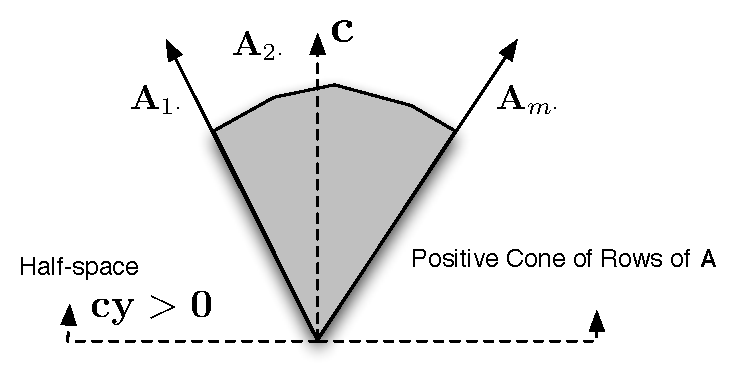
\includegraphics[scale=0.75]{System2.pdf}
\caption{System 2 has a solution if (and only if) the vector $\mathbf{c}$ is contained inside the positive cone constructed from the rows of $\mathbf{A}$. }
\label{fig:System2}
\end{figure}
On the other hand, suppose System 1 has a solution. Then let $\mathbf{y} = -\mathbf{x}$. System 1 states that $\mathbf{A}\mathbf{y} \leq \mathbf{0}$ and $\mathbf{c}\mathbf{y} > 0$. That means that each row of $\mathbf{A}$ (as a vector) must be at a right angle or obtuse to $\mathbf{y}$. (Since $\mathbf{A}_{i \cdot}\mathbf{x} \geq \mathbf{0}$.) Further, we know that the vector $\mathbf{y}$ must be acute with respect to the vector $\mathbf{c}$. This means that System 1 has a solution only if the vector $\mathbf{c}$ is not in the positive cone of the rows of $\mathbf{A}$ or equivalently the intersection of the open half-space $\{\mathbf{y} : \mathbf{c}\mathbf{y} > 0\}$ and the set of vectors $\{\mathbf{y} : \mathbf{A}_{i\cdot}\mathbf{y} \leq \mathbf{0}, i=1,\dots m\}$ is non-empty. This set is the cone of vectors perpendicular to the rows of $\mathbf{A}$. This is illustrated in Figure \ref{fig:System1}
\begin{figure}[htbp]
\centering
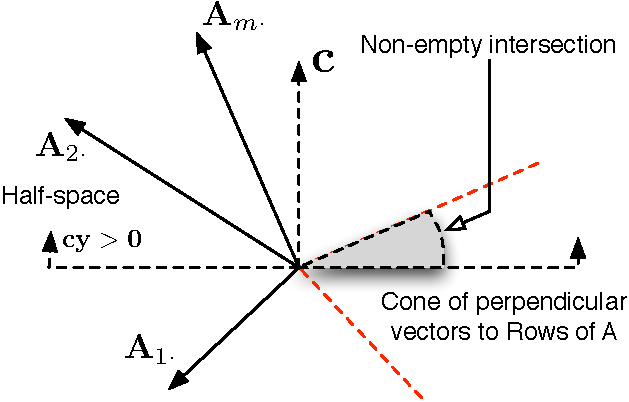
\includegraphics[scale=0.75]{System1.pdf}
\caption{System 1 has a solution if (and only if) the vector $\mathbf{c}$ is not contained inside the positive cone constructed from the rows of $\mathbf{A}$.}
\label{fig:System1}
\end{figure}
\begin{example} Consider the matrix:
\begin{displaymath}
\mathbf{A} = \begin{bmatrix}
1 & 0\\
0 & 1
\end{bmatrix}
\end{displaymath}
and the vector $\mathbf{c} = \begin{bmatrix}1 & 2\end{bmatrix}$. Then clearly, we can see that the vector $\mathbf{w} = \begin{bmatrix}1 & 2\end{bmatrix}$ will satisfy System 2 of Farkas' Lemma, since $\mathbf{w} \geq \mathbf{0}$ and $\mathbf{w}\mathbf{A} = \mathbf{c}$. 

Contrast this with $\mathbf{c}' = \begin{bmatrix}1 & -1\end{bmatrix}$. In this case, we can choose $\mathbf{x} = \begin{bmatrix}0 & 1\end{bmatrix}^T$. Then $\mathbf{A}\mathbf{x} = \begin{bmatrix}0 & 1\end{bmatrix}^T \geq \mathbf{0}$ and $\mathbf{c}'\mathbf{x} = -1$. Thus $\mathbf{x}$ satisfies System 1 of Farkas' Lemma.

These two facts are illustrated in Figure \ref{fig:FarkasExample}. Here, we see that $\mathbf{c}$ is inside the positive cone formed by the rows of $\mathbf{A}$, while $\mathbf{c}'$ is not. 
\begin{figure}[ht]
\centering
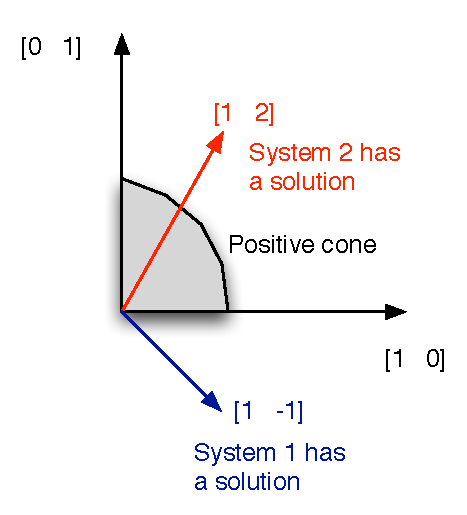
\includegraphics[scale=0.5]{ExampleFarkas.pdf}
\caption{An example of Farkas' Lemma: The vector $\mathbf{c}$ is inside the positive cone formed by the rows of $\mathbf{A}$, but $\mathbf{c}'$ is not.}
\label{fig:FarkasExample} 
\end{figure}
\end{example}

\begin{exercise} Consider the following matrix: 
\begin{displaymath}
\mathbf{A} = \begin{bmatrix}
1 & 0\\
1 & 1
\end{bmatrix}
\end{displaymath}
and the vector $\mathbf{c} = \begin{bmatrix}1 & 2\end{bmatrix}$. For this matrix and this vector, does System 1 have a solution or does System 2 have a solution? [Hint: Draw a picture illustrating the positive cone formed by the rows of $\mathbf{A}$. Draw in $\mathbf{c}$. Is $\mathbf{c}$ in the cone or not?]
\end{exercise}

\subsection{Theorems of the Alternative}
Farkas' lemma can be manipulated in many ways to produce several equivalent statements. The collection of all such theorems are called \textit{Theorems of the Alternative} and are used \textit{extensively} in optimization theory in proving optimality conditions. We state two that will be useful to us.

\begin{corollary} Let $\mathbf{A} \in \mathbb{R}^{k \times n}$ and $\mathbf{E} \in \mathbb{R}^{l \times n}$.  Let $\mathbf{c} \in \mathbb{R}^n$ be a row vector. Suppose $\mathbf{d} \in \mathbb{R}^n$ is a column vector and $\mathbf{w} \in \mathbb{R}^k$ is a row vector and $\mathbf{v} \in \mathbf{R}^{l}$ is a row vector.  Let:
\begin{displaymath}
\mathbf{M} = \begin{bmatrix}
\mathbf{A}\\
\mathbf{E}
\end{bmatrix}
\end{displaymath}
and
\begin{displaymath}
\mathbf{u} = \begin{bmatrix}
\mathbf{w} & \mathbf{v}
\end{bmatrix}
\end{displaymath}
Then exactly one of the following systems has a solution:
\begin{enumerate}
\item $\mathbf{M}\mathbf{d} \leq \mathbf{0}$ and $\mathbf{c}\mathbf{d} > 0$ \textit{or}
\item $\mathbf{u}\mathbf{M} = \mathbf{c}$ and $\mathbf{u}\geq \mathbf{0}$
\end{enumerate}
\label{cor:KKT}
\end{corollary}
\begin{proof} Let $\mathbf{x} = -\mathbf{d}$. Then $\mathbf{M}\mathbf{d} \leq \mathbf{0}$ implies $\mathbf{M}\mathbf{x} \geq \mathbf{0}$ and $\mathbf{c}\mathbf{d} > 0$ implies $\mathbf{c}\mathbf{x} < 0$. This converts System 1 to the System 1 of Farkas' Lemma. System 2 is already in the form found in Farkas' Lemma. This completes the proof. 
\end{proof}

%\begin{exercise} Proof the following corollary to Farkas' Lemma: Let $\mathbf{A} \in \mathbb{R}^{m \times n}$ and $\mathbf{c} \in \mathbb{R}^n$ be a row vector. Suppose $\mathbf{y} \in \mathbb{R}^n$ is a column vector and $\mathbf{w} \in \mathbb{R}^m$ is a row vector. Exactly one of the following two systems has a solution:
%\begin{enumerate}
%\item $\mathbf{A}\mathbf{y} \leq \mathbf{0}$, $\mathbf{y} \leq \mathbf{0}$ and $\mathbf{c}\mathbf{y} > 0$
%\item $\mathbf{w}\mathbf{A}\leq \mathbf{c}$ and $\mathbf{w}\geq \mathbf{0}$
%\end{enumerate}
%[Hint: This is an example in the \cite{BJS04}.]
%\end{exercise}
\begin{exercise} Prove the following corollary to Farkas' Lemma:
\begin{corollary} Let $\mathbf{A} \in \mathbb{R}^{m \times n}$ and $\mathbf{c} \in \mathbb{R}^n$ be a row vector. Suppose $\mathbf{d} \in \mathbb{R}^n$ is a column vector and $\mathbf{w} \in \mathbb{R}^m$ is a row vector and $\mathbf{v} \in \mathbf{R}^{n}$ is a row vector. Then exactly one of the following systems of inequalities has a solution:
\begin{enumerate}
\item $\mathbf{A}\mathbf{d} \leq \mathbf{0}$, $\mathbf{d} \geq \mathbf{0}$ and $\mathbf{c}\mathbf{d} > 0$ \textit{or}
\item $\mathbf{w}\mathbf{A} - \mathbf{v} = \mathbf{c}$ and $\mathbf{w}, \mathbf{v} \geq \mathbf{0}$
\end{enumerate}
\end{corollary}
[Hint: Write System 2 from this corollary as $\mathbf{w}\mathbf{A} - \mathbf{I}_n \mathbf{v} = \mathbf{c}$ and then re-write the system with an augmented vector $[\mathbf{w}\;\;\;\mathbf{v}]$ with an appropriate augmented matrix. Let $\mathbf{M}$ be the augmented matrix you identified. Now write System 1 from Farkas' Lemma using $\mathbf{M}$ and $\mathbf{x}$. Let $\mathbf{d} = -\mathbf{x}$ and expand System 1 until you obtain System 1 for this problem.]
%\begin{proof} Our objective is to transform these systems into something that looks like the systems of Farkas' Lemma. Consider System 2. We may write the equality as:
%\begin{equation}
%\mathbf{w}\mathbf{A} - \mathbf{I}_n \mathbf{v} = \mathbf{c} \iff 
%\begin{bmatrix}\mathbf{w} & \mathbf{v}\end{bmatrix}\begin{bmatrix}\mathbf{A}\\-\mathbf{I}_n\end{bmatrix} = \mathbf{c}
%\end{equation} 
%Define:
%\begin{gather*}
%\mathbf{z} = \begin{bmatrix}\mathbf{w} & \mathbf{v}\end{bmatrix}\\
%\mathbf{M} = \begin{bmatrix}\mathbf{A}\\-\mathbf{I}_n\end{bmatrix}
%\end{gather*}
%Then System 2 is equivalent to: $\mathbf{z}\mathbf{M} = \mathbf{c}$ and $\mathbf{z} \geq \mathbf{0}$. We can now apply Farkas' Lemma to this system. In that case, System 1 becomes: $\mathbf{M}\mathbf{x} \geq \mathbf{0}$ and $\mathbf{c}\mathbf{x} < 0$. For $\mathbf{x} \in \mathbb{R}^{n}$. 
%
%Apply the definition of $\mathbf{M}$ we have:
%\begin{equation}
%\mathbf{M}\mathbf{x} \geq \mathbf{0} \iff \begin{bmatrix}\mathbf{A}\\-\mathbf{I}_n\end{bmatrix}\mathbf{x} \geq \mathbf{0}
%\end{equation}
%The previous equation implies the following system of inequalities:
%\begin{gather}
%\mathbf{A}\mathbf{x} \geq \mathbf{0}\\
%-\mathbf{I}_n\mathbf{x} \geq \mathbf{0}
%\end{gather}
%Let $\mathbf{d} = -\mathbf{x}$. Then we have:
%\begin{displaymath}
%\begin{aligned}
%&\mathbf{A}(-\mathbf{d}) \geq \mathbf{0} \iff \mathbf{A}\mathbf{d} \leq \mathbf{0}\\
%&-\mathbf{I}_n(-\mathbf{d}) \geq \mathbf{0} \iff \mathbf{I}_n\mathbf{d} \geq \mathbf{0} \iff \mathbf{d} \geq \mathbf{0}
%\end{aligned}
%\end{displaymath}
%Lastly, $\mathbf{c}\mathbf{x} < 0$ becomes $\mathbf{c}(-\mathbf{d}) < 0$ or $\mathbf{c}\mathbf{d} > 0$. 
%
%Thus we have shown (by Farkas' Lemma) that either System 1 or System 2 has a solution. This completes the proof.
%\end{proof}
\end{exercise}

\section{The Karush-Kuhn-Tucker Conditions}
\begin{theorem} Consider the linear programming problem:
\begin{equation}
P\left\{
\begin{aligned}
\max\;\; & \mathbf{c}\mathbf{x}\\
s.t.\;\; & \mathbf{A}\mathbf{x} \leq \mathbf{b}\\
& \mathbf{x} \geq \mathbf{0}
\end{aligned}\right.
\end{equation}
with $\mathbf{A} \in \mathbb{R}^{m \times n}$, $\mathbf{b} \in \mathbb{R}^m$ and (row vector) $\mathbf{c} \in \mathbb{R}^n$. Then $\mathbf{x}^* \in \mathbb{R}^n$ is an optimal solution\footnote{Thanks to Rich Benjamin for pointing out the fact I was missing ``\dots is an optimal solution\dots''} to $P$ if and only if there exists (row) vectors $\mathbf{w}^* \in \mathbb{R}^m$ and $\mathbf{v}^* \in \mathbb{R}^n$ so that:
\begin{align}
\text{Primal Feasibility}&\left\{ 
\begin{aligned}
\mathbf{A}\mathbf{x}^* \leq \mathbf{b}\\
\mathbf{x}^* \geq \mathbf{0}
\end{aligned}\right.\\
\text{Dual Feasibility}&\left\{ 
\begin{aligned}
\mathbf{w}^*\mathbf{A} - \mathbf{v}^* = \mathbf{c}\\
\mathbf{w}^* \geq \mathbf{0}\\
\mathbf{v}^* \geq \mathbf{0}
\end{aligned}\right.\\
\text{Complementary Slackness}&\left\{ 
\begin{aligned}
\mathbf{w}^*\left(\mathbf{A}\mathbf{x}^* - \mathbf{b}\right) = 0\\
\mathbf{v}^*\mathbf{x}^* = 0
\end{aligned}\right.
\end{align}
\label{thm:KKT}
\end{theorem}
\begin{remark} The vectors $\mathbf{w}^*$ and $\mathbf{v}^*$ are sometimes called \textit{dual variables} for reasons that will be clear in the next chapter. They are also sometimes called \textit{Lagrange Multipliers}. You may have encountered Lagrange Multipliers in your Math 230 or Math 231 class. These are the same kind of variables except applied to linear optimization problems. 
There is one element in the dual variable vector $\mathbf{w}^*$ for each constraint of the form $\mathbf{A}\mathbf{x} \leq \mathbf{b}$ and one element in the dual variable vector $\mathbf{v}^*$ for each constraint of the form $\mathbf{x} \geq \mathbf{0}$. 
\end{remark}
\begin{proof} Suppose that $\mathbf{x}^*$ is an optimal solution to Problem $P$. Consider only the \textit{binding constraints} at $\mathbf{x}^*$. For simplicity, write the constraints $\mathbf{x} \geq \mathbf{0}$ as $-\mathbf{x} \leq \mathbf{0}$. Then we can form a new system of equations of the form:
\begin{align}
\begin{bmatrix} \mathbf{A}_E \\ \mathbf{E} \end{bmatrix} \mathbf{x} = \mathbf{b}_E
\end{align}
where $\mathbf{E}$ is a matrix of negative identity matrix rows corresponding to the variables $x_k$ that are equal to zero. That is, if $x_k = 0$, then $-x_k = 0$ and the negative identity matrix row $-\mathbf{e}^T_k$ will appear in $\mathbf{E}$ where $-\mathbf{e}^T_k \in \mathbb{R}^{1 \times n}$. Here $\mathbf{b}_\mathbf{E}$ are the right hand sides of the binding constraints. Let:
\begin{displaymath}
\mathbf{M} = \begin{bmatrix}
\mathbf{A}_E\\
\mathbf{E}
\end{bmatrix}
\end{displaymath}
The fact that $\mathbf{x}^*$ is optimal implies that there is no improving direction $\mathbf{d}$ at the point $\mathbf{x}^*$. That is, there is no $\mathbf{d}$ so that $\mathbf{M}\mathbf{d} \leq \mathbf{0}$ and $\mathbf{c}^T\mathbf{d} > 0$. Otherwise, by moving in this direction we could find a new point $\hat{\mathbf{x}} = \mathbf{x}^* + \lambda\mathbf{d}$ (with $\lambda$ sufficiently small) so that:
\begin{displaymath}
\mathbf{M}\hat{\mathbf{x}} = \mathbf{M}\mathbf{x}^* + \lambda \mathbf{M}\mathbf{d} \leq \mathbf{b}_E
\end{displaymath}
The (negative) identity rows in $\mathbf{E}$ ensure that $\hat{\mathbf{x}} \geq \mathbf{0}$. 
It follows that:
\begin{displaymath}
\mathbf{c}\hat{\mathbf{x}} = \mathbf{c}^T\left( \mathbf{x}^* + \lambda\mathbf{d}\right) = \mathbf{c}\mathbf{x}^* + \lambda\mathbf{c}\mathbf{d} > \mathbf{c}\mathbf{x}^*
\end{displaymath}
That is, this point is both feasible and has a larger objective function value than $\mathbf{x}^*$. 

We can now apply Corollary \ref{cor:KKT} to show that there are vectors $\mathbf{w}$ and $\mathbf{v}$ so that:
\begin{align}
\begin{bmatrix}\mathbf{w} & \mathbf{v}\end{bmatrix}
\begin{bmatrix}
\mathbf{A}_E \\
\mathbf{E}\label{eqn:DualFeas1}
\end{bmatrix} = \mathbf{c}\\
\mathbf{w} \geq \mathbf{0}\\
\mathbf{v} \geq \mathbf{0}
\end{align}

Let $I$ be the indices of the rows of $\mathbf{A}$ making up $\mathbf{A}_E$ and let $J$ be the indices of the variables that are zero (i.e., binding in $\mathbf{x} \geq \mathbf{0}$). Then we can re-write Equation \ref{eqn:DualFeas1} as:
\begin{equation}
\sum_{i \in I} w_i \mathbf{A}_{i\cdot} - \sum_{j \in J} v_j \mathbf{e}_j = \mathbf{c}
\label{eqn:ConversePart}
\end{equation}
The vector $\mathbf{w}$ has dimension equal to the number of binding constraints of the form $\mathbf{A}_{i\cdot}\mathbf{x} = \mathbf{b}$ while the vector $\mathbf{v}$ has dimension equal to the number of binding constraints of the form $\mathbf{x} \geq \mathbf{0}$. We can extend $\mathbf{w}$ to $\mathbf{w}^*$ by adding $0$ elements for the constraints where $\mathbf{A}_{i\cdot}\mathbf{x} < \mathbf{b}_i$. Similarly we can extend $\mathbf{v}$ to $\mathbf{v}^*$ by adding $0$ elements for the constraints where $x_j > 0$. The result is that:
\begin{align}
\mathbf{w}^*\left(\mathbf{A}\mathbf{x}^* - \mathbf{b}\right) = 0\\
\mathbf{v}^*\mathbf{x}^* = 0
\end{align}
In doing this we maintain $\mathbf{w}^*,\mathbf{v}^* \geq \mathbf{0}$ and simultaneously guarantee that $\mathbf{w}^* \mathbf{A} - \mathbf{v}^* = \mathbf{c}$. 

To prove the converse we assume that the KKT conditions hold and we are given vectors $\mathbf{x}^*$, $\mathbf{w}^*$ and $\mathbf{v}^*$. We will show that $\mathbf{x}^*$ solves the linear programming problem. By dual feasibility, we know that Equation \ref{eqn:ConversePart} holds with $\mathbf{w} \geq \mathbf{0}$ and $\mathbf{v} \geq \mathbf{0}$ defined as before and the given point $\mathbf{x}^*$. Let $\mathbf{x}$ be an alternative point. 
We can multiply both side of Equation \ref{eqn:ConversePart} by $(\mathbf{x}^* - \mathbf{x})$. This leads to:
\begin{equation}
\left\{\sum_{i \in I} w_i \mathbf{A}_{i\cdot}\mathbf{x}^* - \sum_{j \in J} v_j \mathbf{e}_j\mathbf{x}^*\right\}- 
\left\{\sum_{i \in I} w_i \mathbf{A}_{i\cdot}\mathbf{x} - \sum_{j \in J} v_j \mathbf{e}_j\mathbf{x}^* \right\} = \mathbf{c}\mathbf{x}^* - \mathbf{c}\mathbf{x}
\label{eqn:KKTMiddle}
\end{equation}
We know that $\mathbf{A}_{i\cdot}\mathbf{x}^* = \mathbf{b}_i$ for $i \in I$ and that $x^*_j = 0$ for $j \in J$. We can use this to simplify Equation \ref{eqn:KKTMiddle}:
\begin{equation}
\sum_{i \in I} w_i \left(\mathbf{b}_i - \mathbf{A}_{i\cdot}\mathbf{x}\right) + \sum_{j \in J} v_j \mathbf{e}_j\mathbf{x} = \mathbf{c}\mathbf{x}^* - \mathbf{c}\mathbf{x}
\end{equation}
The left hand side must be non-negative, since $\mathbf{w} \geq \mathbf{0}$ and $\mathbf{v} \geq \mathbf{0}$, $b_i - \mathbf{A}_{i\cdot}\mathbf{x} \geq 0$ for all $i$, and $\mathbf{x} \geq 0$ and thus it follows that $\mathbf{x}^*$ must be an optimal point since $\mathbf{c}\mathbf{x}^* - \mathbf{c}\mathbf{x} \geq 0$. This completes the proof.
\end{proof}
\begin{remark} The expressions:
\begin{align}
\text{Primal Feasibility}&\left\{ 
\begin{aligned}
\mathbf{A}\mathbf{x}^* \leq \mathbf{b}\\
\mathbf{x}^* \geq \mathbf{0}
\end{aligned}\right.\\
\text{Dual Feasibility}&\left\{ 
\begin{aligned}
\mathbf{w}^*\mathbf{A} - \mathbf{v}^* = \mathbf{c}\\
\mathbf{w}^* \geq \mathbf{0}\\
\mathbf{v}^* \geq \mathbf{0}
\end{aligned}\right.\\
\text{Complementary Slackness}&\left\{ 
\begin{aligned}
\mathbf{w}^*\left(\mathbf{A}\mathbf{x}^* - \mathbf{b}\right) = 0\\
\mathbf{v}^*\mathbf{x}^* = 0
\end{aligned}\right.
\end{align}
are called the \textit{Karush-Kuhn-Tucker (KKT) conditions} of optimality. Note there is one element in $\mathbf{w}$ for each row of the constraints $\mathbf{A}\mathbf{x} \leq \mathbf{b}$ and one element in the vector $\mathbf{v}$ for each constraint of the form $\mathbf{x} \geq \mathbf{0}$. The vectors $\mathbf{w}$ and $\mathbf{v}$ are sometimes called \textit{dual variables} and sometimes called Lagrange Multipliers.

We can think of dual feasibility as expressing the following interesting fact: at optimality, the gradient of the objective function $\mathbf{c}$ can be expressed as a positive combination of the gradients of the binding constraints written as less-than-or-equal-to inequalities. That is, the gradient of the constraint $\mathbf{A}_{i\cdot}\mathbf{x} \leq \mathbf{b}_i$ is $\mathbf{A}_{i\cdot}$ and the gradient of the constraint $-{x}_j \leq 0$ is $-\mathbf{e}_j$. More specifically, the vector $\mathbf{c}$ is in the \textit{cone} generated by the binding constraints at optimality. 
\end{remark}

\begin{example}
Consider the Toy Maker Problem (Equation \ref{eqn:ToyMakerEx}) with Dual Variables (Lagrange Multipliers) listed next to their corresponding constraints:
\begin{displaymath}
\left\{
\begin{aligned}
\max\;\;& z(x_1,x_2) = 7x_1 + 6x_2 & \quad \text{\textbf{Dual Variable}}\\
s.t.\;\;&  3x_1 + x_2 \leq 120 & \quad (w_1)\\
& x_1 + 2x_2 \leq 160 & \quad (w_1)\\
& x_1 \leq 35 & \quad (w_3)\\
& x_1 \geq 0 & \quad (v_1)\\
& x_2 \geq 0 & \quad (v_2)
\end{aligned}
\right.
\end{displaymath}
In this problem we have:
\begin{displaymath}
\mathbf{A} = \begin{bmatrix}
3 & 1\\
1 & 2 \\
1 & 0
\end{bmatrix}\quad \mathbf{b} = \begin{bmatrix}120\\160\\35\end{bmatrix} \quad
\mathbf{c} = \begin{bmatrix}7 & 6\end{bmatrix}
\end{displaymath}
Then the KKT conditions can be written as:
\begin{displaymath}
\text{Primal Feasibility}\left\{
\begin{aligned}
& \begin{bmatrix}
3 & 1\\
1 & 2 \\
1 & 0
\end{bmatrix}\begin{bmatrix}x_1\\x_2\end{bmatrix} \leq \begin{bmatrix}120\\160\\35\end{bmatrix}\\
& \begin{bmatrix}x_1\\x_2\end{bmatrix} \geq \begin{bmatrix}0\\0\end{bmatrix}
\end{aligned}\right.
\end{displaymath}
\begin{displaymath}
\text{Dual Feasibility}\left\{
\begin{aligned}
& \begin{bmatrix}w_1&w_2&w_3\end{bmatrix}\begin{bmatrix}
3 & 1\\
1 & 2 \\
1 & 0
\end{bmatrix} - \begin{bmatrix}v_1 & v_2\end{bmatrix} = \begin{bmatrix}7 & 6\end{bmatrix}\\
& \begin{bmatrix}w_1&w_2&w_3\end{bmatrix} \geq \begin{bmatrix}0&0&0\end{bmatrix}\\
& \begin{bmatrix}v_1&v_2\end{bmatrix} \geq \begin{bmatrix}0&0\end{bmatrix}
\end{aligned}\right.
\end{displaymath}
\begin{displaymath}
\text{Complementary Slackness}\left\{
\begin{aligned}
& \begin{bmatrix}w_1&w_2&w_3\end{bmatrix}\left( \begin{bmatrix}
3 & 1\\
1 & 2 \\
1 & 0
\end{bmatrix}\begin{bmatrix}x_1\\x_2\end{bmatrix} \leq \begin{bmatrix}120\\160\\35\end{bmatrix} - \begin{bmatrix}120\\160\\35\end{bmatrix}\right)\\
& \begin{bmatrix}v_1&v_2\end{bmatrix} \begin{bmatrix}x_1&x_2\end{bmatrix} = 0
\end{aligned}\right.
\end{displaymath}
Recall that at optimality, we had $x_1 = 16$ and $x_2 = 72$. The binding constraints in this case where 
\begin{gather*}
3x_1 + x_2 \leq 120\\
x_1 + 2x_2 \leq 160
\end{gather*}
To see this note that if $3(16)+72 = 120$ and $16+2(72) = 160$. Then we should be able to express $\mathbf{c} = [7\;\;\;6]$ (the vector of coefficients of the objective function) as a positive combination of the gradients of the binding constraints:
\begin{gather*}
\nabla(7x_1 + 6x_2) = \begin{bmatrix}7 & 6\end{bmatrix}\\
\nabla(3x_1 + x_2) = \begin{bmatrix}3 & 1\end{bmatrix}\\
\nabla(x_1 + 2x_2) = \begin{bmatrix}1 & 2\end{bmatrix}
\end{gather*}
That is, we wish to solve the linear equation:
\begin{equation}
\begin{bmatrix}w_1 & w_2\end{bmatrix}\begin{bmatrix}3 & 1\\1 & 2\end{bmatrix} = \begin{bmatrix}7 & 6\end{bmatrix}
\end{equation}
Note, this is how Equation \ref{eqn:ConversePart} looks when we apply it to this problem. The result is a system of equations:
\begin{gather*}
3w_1 + w_2 = 7\\
w_1 + 2w_2 = 6
\end{gather*}
A solution to this system is $w_1 = \frac{8}{5}$ and $w_2 =\frac{11}{5}$. This fact is illustrated in Figure \ref{fig:GradientCone}. 

Figure \ref{fig:GradientCone} shows the gradient cone formed by the binding constraints at the optimal point for the toy maker problem. 
\begin{figure}[htbp]
\centering
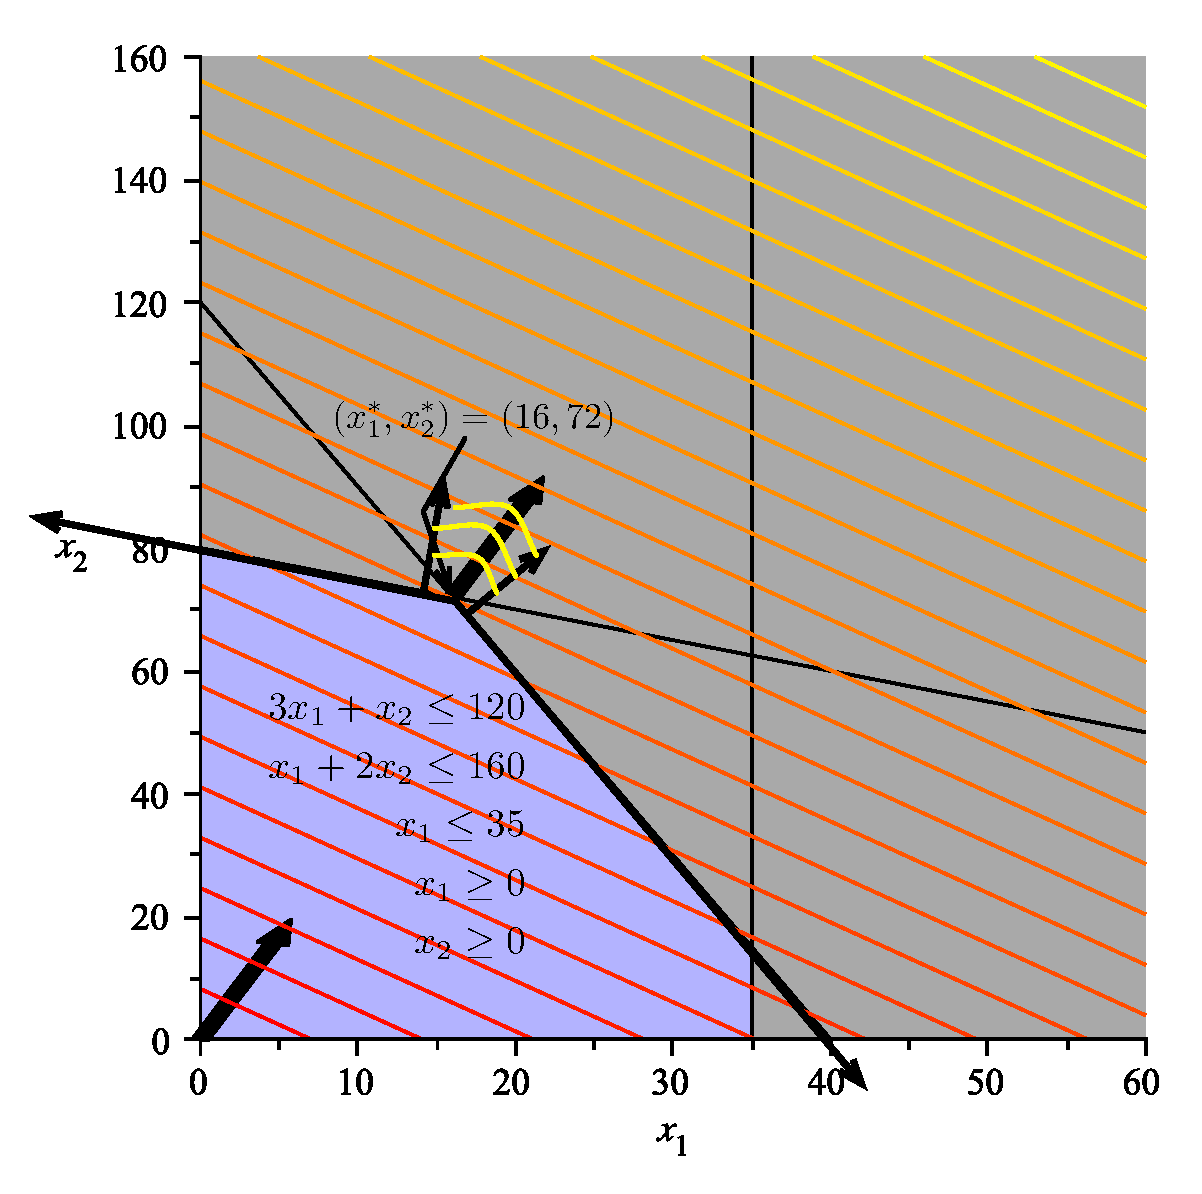
\includegraphics[scale=0.35]{GradientCone.pdf}
\caption{The Gradient Cone: At optimality, the cost vector $\mathbf{c}$ is obtuse with respect to the directions formed by the binding constraints. It is also contained inside the cone of the gradients of the binding constraints, which we will discuss at length later.}
\label{fig:GradientCone}
\end{figure}
Since $x_1, x_2 > 0$, we must have $v_1 = v_2 = 0$. Moreover, since $x_1 < 35$, we know that $x_1 \leq 35$ is not a binding constraint and thus its dual variable $w_3$ is also zero. This leads to the conclusion:
\begin{displaymath}
\begin{bmatrix}
x_1^*\\
x_2^*
\end{bmatrix} = \begin{bmatrix}
16\\
72
\end{bmatrix} \quad 
\begin{bmatrix}
w_1^* & w_2^* & w_3^*
\end{bmatrix} = \begin{bmatrix}8/5 & 11/5 & 0\end{bmatrix} \quad \begin{bmatrix} v_1^* & v_2^*\end{bmatrix} = \begin{bmatrix}0 & 0\end{bmatrix}
\end{displaymath}
and the KKT conditions are satisfied.
\end{example}

\begin{exercise} Consider the problem:
\begin{displaymath}
\begin{aligned}
\max\;\;&x_1 + x_2\\
s.t.\;\;&2x_1 + x_2 \leq 4\\
&x_1 + 2x_2 \leq 6\\
&x_1, x_2 \geq 0
\end{aligned}
\end{displaymath}
Write the KKT conditions for an optimal point for this problem. (You will have a vector $\mathbf{w} = [w_1 \;\;\; w_2]$ and a vector $\mathbf{v} = [v_1\;\;\;v_2]$). 

Draw the feasible region of the problem. At the optimal point you identified in Exercise \ref{exer:RevisedSimplex}, identify the binding constraints and draw their gradients. Show that the objective function is in the positive cone of the gradients of the binding constraints at this point. (Specifically find $\mathbf{w}$ and $\mathbf{v}$.)
\label{exer:FindKKT}
\end{exercise}

\subsection*{The Karush-Kuhn-Tucker Conditions for an Equality Problem}
The KKT conditions can be modified to deal with problems in which we have equality constraints (i.e., $\mathbf{A}\mathbf{x} = \mathbf{b}$).

\begin{corollary} Consider the linear programming problem:
\begin{equation}
P\left\{
\begin{aligned}
\max\;\; & \mathbf{c}\mathbf{x}\\
s.t.\;\; & \mathbf{A}\mathbf{x} = \mathbf{b}\\
& \mathbf{x} \geq \mathbf{0}
\end{aligned}\right.
\end{equation}
with $\mathbf{A} \in \mathbb{R}^{m \times n}$, $\mathbf{b} \in \mathbb{R}^m$ and (row vector) $\mathbf{c} \in \mathbb{R}^n$. Then $\mathbf{x}^* \in \mathbb{R}^n$ if and only if there exists (row) vectors $\mathbf{w}^* \in \mathbb{R}^m$ and $\mathbf{v}^* \in \mathbb{R}^n$ so that:
\begin{align}
\text{Primal Feasibility}&\left\{ 
\begin{aligned}
\mathbf{A}\mathbf{x}^* = \mathbf{b}\\
\mathbf{x}^* \geq \mathbf{0}
\end{aligned}\right.\\
\text{Dual Feasibility}&\left\{ 
\begin{aligned}
\mathbf{w}^*\mathbf{A} - \mathbf{v}^* = \mathbf{c}\\
\mathbf{w}^* \text{ unrestricted}\\
\mathbf{v}^* \geq \mathbf{0}
\end{aligned}\right.\\
\text{Complementary Slackness}&\left\{ 
\begin{aligned}
\mathbf{v}^*\mathbf{x}^* = 0
\end{aligned}\right.
\end{align}
\end{corollary}
\begin{proof} Replace the constraints $\mathbf{A}\mathbf{x} = \mathbf{b}$ with the equivalent constraints:
\begin{align}
\mathbf{A}\mathbf{x} &\leq \mathbf{b}\\
-\mathbf{A}\mathbf{x} &\leq -\mathbf{b}
\end{align}
Let $\mathbf{w}_1$ be the vector corresponding to the rows in $\mathbf{A}\mathbf{x} \leq \mathbf{b}$ and $\mathbf{w}_2$ be the vector corresponding to the rows in $-\mathbf{A}\mathbf{x} \leq -\mathbf{b}$. Then the KKT conditions are:
\begin{align}
\text{Primal Feasibility}&\left\{ 
\begin{aligned}
\mathbf{A}\mathbf{x} &\leq \mathbf{b}\\
-\mathbf{A}\mathbf{x} &\leq -\mathbf{b}\\
\mathbf{x}^* \geq \mathbf{0}
\end{aligned}\right.\\
\text{Dual Feasibility}&\left\{ 
\begin{aligned}
\mathbf{w}_1^*\mathbf{A} -\mathbf{w}_2\mathbf{A}- \mathbf{v}^* = \mathbf{c}\\
\mathbf{w}_1^* \geq \mathbf{0}\\
\mathbf{w}_2^* \geq \mathbf{0}\\
\mathbf{v}^* \geq \mathbf{0}
\end{aligned}\right.\\
\text{Complementary Slackness}&\left\{ 
\begin{aligned}
\mathbf{w}_1^*\left(\mathbf{A}\mathbf{x}^* - \mathbf{b}\right) = 0\\
\mathbf{w}_2^*\left(\mathbf{b} - \mathbf{A}\mathbf{x}^*\right) = 0\\
\mathbf{v}^*\mathbf{x}^* = 0
\end{aligned}\right.
\end{align}
The fact that $\mathbf{A}\mathbf{x} = \mathbf{b}$ at optimality ensures we can re-write primal-feasibility as:
\begin{align*}
\text{Primal Feasibility}&\left\{ 
\begin{aligned}
\mathbf{A}\mathbf{x} = \mathbf{b}\\
\mathbf{x}^* \geq \mathbf{0}
\end{aligned}\right.
\end{align*}
Furthermore, since $\mathbf{A}\mathbf{x} = \mathbf{b}$ we know that complementary slackness of
\begin{align*}
\begin{aligned}
\mathbf{w}_1^*\left(\mathbf{A}\mathbf{x}^* - \mathbf{b}\right) = 0\\
\mathbf{w}_2^*\left(\mathbf{b} - \mathbf{A}\mathbf{x}^*\right) = 0
\end{aligned}
\end{align*}
is always satisfied and thus, we only require $\mathbf{v}^*\mathbf{x}^* = 0$ as our complementary slackness condition.

Finally, let $\mathbf{w} = \mathbf{w_1} - \mathbf{w}_2$. Then dual feasibility becomes:
\begin{equation}
\mathbf{w}\mathbf{A} - \mathbf{v} = \mathbf{w}_1^*\mathbf{A} -\mathbf{w}_2\mathbf{A}- \mathbf{v}^* = \mathbf{c}
\end{equation}
Since $\mathbf{w}_1,\mathbf{w}_2 \geq \mathbf{0}$, we know that $\mathbf{w}$ is unrestricted in sign. Thus we have:
\begin{align}
\text{Dual Feasibility}&\left\{ 
\begin{aligned}
\mathbf{w}\mathbf{A} - \mathbf{v}^* = \mathbf{c}\\
\mathbf{w}^* \text{ unrestricted}\\
\mathbf{v}^* \geq \mathbf{0}
\end{aligned}\right.
\end{align}
This completes the proof.
\end{proof}

\begin{exercise} Use the trick of converting a minimization problem to a maximization problem to identify the KKT conditions for the following problem:
\begin{equation}
\begin{aligned}
\min\;\; & \mathbf{c}\mathbf{x}\\
s.t.\;\;& \mathbf{A}\mathbf{x} \geq \mathbf{b}\\
& \mathbf{x} \geq \mathbf{0}
\end{aligned}
\end{equation}
[Hint: Remember, $\mathbf{A}\mathbf{x} \geq \mathbf{b}$ is the same as writing $-\mathbf{A}\mathbf{x} \leq -\mathbf{b}$. Now use the KKT conditions for the maximization problem to find the KKT conditions for this problem.]
\label{exer:MinKKT}
\end{exercise}

\section{Relating the KKT Conditions to the Tableau}
Consider a linear programming problem in Standard Form:
\begin{equation}
P\left\{
\begin{aligned}
\max\;\; & \mathbf{c}\mathbf{x}\\
s.t.\;\; & \mathbf{A}\mathbf{x} = \mathbf{b}\\
& \mathbf{x} \geq \mathbf{0}
\end{aligned}\right.
\end{equation}
with $\mathbf{A} \in \mathbb{R}^{m \times n}$, $\mathbf{b} \in \mathbb{R}^m$ and (row vector) $\mathbf{c} \in \mathbb{R}^n$.

The KKT conditions for a problem of this type assert that
\begin{gather*}
\mathbf{w}\mathbf{A} - \mathbf{v} = \mathbf{c}\\
\mathbf{v}\mathbf{x}= 0
\end{gather*}
at an optimal point $\mathbf{x}$ for some vector $\mathbf{w}$ unrestricted in sign and $\mathbf{v} \geq \mathbf{0}$. (Note, for the sake of notational ease, we have dropped the $^*$ notation.)

Suppose at optimality we have a basis matrix $\mathbf{B}$ corresponding to a set of basic variables $\mathbf{x}_\mathbf{B}$ and we simultaneously have non-basic variables $\mathbf{x}_\mathbf{N}$. We may likewise divide $\mathbf{v}$ into $\mathbf{v}_\mathbf{B}$ and $\mathbf{v}_\mathbf{N}$. 

Then we have:
\begin{equation}
\mathbf{w}\mathbf{A} - \mathbf{v} = \mathbf{c} \implies 
\mathbf{w}\begin{bmatrix}\mathbf{B} & \mathbf{N}\end{bmatrix} - \begin{bmatrix}\mathbf{v}_\mathbf{B} & \mathbf{v}_\mathbf{N}\end{bmatrix} = 
\begin{bmatrix}\mathbf{c}_\mathbf{B} & \mathbf{c}_\mathbf{N}\end{bmatrix}\label{eqn:TableauRelate1}
\end{equation}
\begin{equation}
\mathbf{v}\mathbf{x} = 0 \implies 
\begin{bmatrix}\mathbf{v}_\mathbf{B} & \mathbf{v}_\mathbf{N}
\end{bmatrix}
\begin{bmatrix}\mathbf{x}_\mathbf{B}\\
\mathbf{x}_\mathbf{N}
\end{bmatrix} = 0\label{eqn:TableauRelate2}
\end{equation}
We can rewrite Expression \ref{eqn:TableauRelate1} as:
\begin{equation}
\begin{bmatrix}
\mathbf{w}\mathbf{B}-\mathbf{v}_\mathbf{B} & 
\mathbf{w}\mathbf{N}-\mathbf{v}_\mathbf{N}
\end{bmatrix} =
\begin{bmatrix}
\mathbf{c}_\mathbf{B} & \mathbf{c}_\mathbf{N}
\end{bmatrix}
\end{equation}
This simplifies to:
\begin{gather*}
\mathbf{w}\mathbf{B} - \mathbf{v}_\mathbf{B} = \mathbf{c}_\mathbf{B}\\
\mathbf{w}\mathbf{N} - \mathbf{v}_\mathbf{N} = \mathbf{c}_\mathbf{N}\\
\end{gather*}
Let $\mathbf{w} = \mathbf{c}_\mathbf{B}\mathbf{B}^{-1}$. Then we see that:
\begin{equation}
\mathbf{w}\mathbf{B} - \mathbf{v}_\mathbf{B} = \mathbf{c}_\mathbf{B} \implies \mathbf{c}_\mathbf{B}\mathbf{B}^{-1}\mathbf{B} - \mathbf{v}_\mathbf{B} = \mathbf{c}_\mathbf{B} \implies \mathbf{c}_\mathbf{B} - \mathbf{v}_\mathbf{B} = \mathbf{c}_\mathbf{B} \implies \mathbf{v}_\mathbf{B} = \mathbf{0}
\end{equation}
Since we know that $\mathbf{x}_\mathbf{B} \geq \mathbf{0}$, we know that $\mathbf{v}_\mathbf{B}$ should be equal to zero to ensure complementary slackness. Thus, this is consistent with the KKT conditions.

We further see that:
\begin{equation}
\mathbf{w}\mathbf{N} - \mathbf{v}_\mathbf{N} = \mathbf{c}_\mathbf{N} \implies
\mathbf{c}_\mathbf{B}\mathbf{B}^{-1}\mathbf{N} - \mathbf{v}_\mathbf{N} = \mathbf{c}_\mathbf{N} \implies 
\mathbf{v}_\mathbf{N} = \mathbf{c}_\mathbf{B}\mathbf{B}^{-1}\mathbf{N} - \mathbf{c}_\mathbf{N}
\end{equation}
Thus, the $\mathbf{v}_\mathbf{N}$ are just the reduced costs of the non-basic variables. ($\mathbf{v}_\mathbf{B}$ are the reduced costs of the basic variables.) Furthermore, dual feasibility requires that $\mathbf{v} \geq \mathbf{0}$. Thus we see that at optimality we require:
\begin{equation}
\mathbf{c}_\mathbf{B}\mathbf{B}^{-1}\mathbf{N} - \mathbf{c}_\mathbf{N} \geq \mathbf{0}
\end{equation}
This is \textit{precisely} the condition for optimality in the simplex tableau. 

We now can see the following facts are true about the Simplex Method:
\begin{enumerate}
\item At each iteration of the Simplex Method, primal feasibility is satisfied. This is ensured by the minimum ratio test and the fact that we start at a feasible point.

\item At each iteration of the Simplex Method, complementary slackness is satisfied. After all, the vector $\mathbf{v}$ is just the reduced cost vector (Row 0) of the Simplex tableau. If a variable is basic $x_j$ (and hence non-zero), then the its reduced cost $v_j = 0$. Otherwise, $v_j$ may be non-zero.

\item At each iteration of the Simplex Algorithm, we may violate dual feasibility because we may not have $\mathbf{v} \geq \mathbf{0}$. It is \textit{only} at optimality that we achieve dual feasibility and satisfy the KKT conditions. 
\end{enumerate}

We can now prove the following theorem:
\begin{theorem} Assuming an appropriate cycling prevention rule is used, the simplex algorithm converges in a finite number of iterations to an optimal solution to the linear programming problem.
\end{theorem}
\begin{proof} Convergence is guaranteed by the proof of Theorem \ref{thm:SimplexConverge} in which we show that when the lexicographic minimum ratio test is used, then the simplex algorithm will always converge. Our work above shows that at optimality, the KKT conditions are satisfied because the termination criteria for the simplex algorithm are precisely the same as the criteria in the Karush-Kuhn-Tucker conditions. This completes the proof.
\end{proof}

\begin{example} Consider the following linear programming problem: 
\begin{displaymath}
\left\{
\begin{aligned}
\max\;\;& z(x_1,x_2) = 3x_1 + 5x_2\\
s.t.\;\;&  x_1 + 2x_2 \leq 60 \quad (w_1)\\
& x_1 + x_2 \leq 40 \quad (w_2)\\
& x_1 \geq 0 \quad(v_1)\\
& x_2 \geq 0 \quad(v_2)
\end{aligned}
\right.
\end{displaymath}
Note we have assigned dual variables corresponding to each constraint on the right-hand-side of the constraints. That is, dual variable $w_1$ corresponds to the constraint $x_1 + 2x_2 \leq 60$. We can write this problem in standard form as:
\begin{displaymath}
\left\{
\begin{aligned}
\max\;\;& z(x_1,x_2) = 3x_1 + 5x_2\\
s.t.\;\;&  x_1 + 2x_2 + s_1 = 60 \quad (w_1)\\
& x_1 + x_2 + s_2 = 40 \quad (w_2)\\
& x_1 \geq 0 \quad(v_1)\\
& x_2 \geq 0 \quad(v_2)\\
& s_1 \geq 0 \quad(v_3)\\
& s_2 \geq 0 \quad(v_4)
\end{aligned}
\right.
\end{displaymath}
Note we have added two new dual variables $v_3$ and $v_4$ for the non-negativity constraints on slack variables $s_1$ and $s_2$. Our dual variable vectors are: $\mathbf{w} = [w_1 \;\; w_2]$ and $\mathbf{v} = [v_1\;\;v_2\;\;v_3\;\;v_4]$. We can construct an initial simplex tableau as:
\begin{displaymath}
\begin{array}{c}
z\\s_1\\s_2
\end{array}
\left[\begin{array}{c|cccc|c}
z & 	x_1 &	x_2 & 	s_1 &	s_2 & 	RHS\\
\hline
1 & 	-3 & 	-5 & 	0 & 	0 & 	0\\
\hline
0 &  	1 & 	2 & 	1 & 	0 & 	60\\
0 & 	1 & 	1 & 	0 & 	1 & 	40
\end{array}\right]
\end{displaymath}
In this initial configuration, we note that $v_1 = -3$, $v_2 = -5$, $v_3 = 0$ and $v_4 = 0$. This is because $s_1$ and $s_2$ are basic variables. We also notice that complementary slackness is satisfied. That is at the current values of $x_1$, $x_2$, $s_1$ and $s_2$ we have:
\begin{displaymath}
\begin{bmatrix}v_1 & v_2 & v_3 & v_4\end{bmatrix}
\begin{bmatrix}x_1 \\ x_2 \\ s_1 \\ s_2\end{bmatrix} = 0
\end{displaymath}
Applying the Simplex Algorithm yields the final tableau:
\begin{displaymath}
\begin{array}{c}
\\
z\\x_2\\x_1
\end{array}
\left[\begin{array}{c|cccc|c}
z & 	x_1 &	x_2 & 	s_1 &	s_2 & 	RHS\\
\hline
1 & 	0 & 	0 & 	2 & 	1 & 	160\\
\hline
0 &  	0 & 	1 & 	\mathbf{1} & 	\mathbf{-1} & 	20\\
0 & 	1 & 	0 & 	\mathbf{-1} & 	\mathbf{2} & 	20
\end{array}\right]
\end{displaymath}
The optimal value for $\mathbf{v}$ is $[0\;\;0\;\;2\;\;1]$. Note $\mathbf{v} \geq \mathbf{0}$ as required. Further, complementary slackness is still maintained. Notice further that the current value of $\mathbf{B}^{-1}$ can be found in the portion of the matrix where the identity matrix stood in the initial tableau. Thus we can compute $\mathbf{w}$ as:
\begin{displaymath}
\mathbf{w} = \mathbf{c}_\mathbf{B}\mathbf{B}^{-1}
\end{displaymath}
Since $\mathbf{c}_\mathbf{B} = [5\;\;3]$ (since $x_2$ and $x_1$ the basic variables at optimality) we see that:
\begin{displaymath}
\mathbf{w} = \begin{bmatrix}5 & 3\end{bmatrix}
\begin{bmatrix}
1 & 	-1\\
-1 & 	2
\end{bmatrix} = \begin{bmatrix}2 & 1\end{bmatrix}
\end{displaymath}
That is, $w_1 = 2$ and $w_2 = 1$. 

Note that $\mathbf{w} \geq \mathbf{0}$. This is because $\mathbf{w}$ is also a dual variable vector for our original problem (not in standard form). The KKT conditions for a maximization problem in canonical form require $\mathbf{w} \geq \mathbf{0}$ (see Theorem \ref{thm:KKT}). Thus, it makes sense that we have $\mathbf{w} \geq \mathbf{0}$. Note this does not always have to be the case if we do not begin with a problem in canonical form. 

Last, we can see that the constraints:
\begin{gather*}
x_1 + 2x_2 \leq 60\\
x_1 + x_2 \leq 40 
\end{gather*}
are both binding at optimality (since $s_1$ and $s_2$ are both zero). This means we should be able to express $\mathbf{c} = [3\;\;5]^T$ as a positive combination of the gradients of the left-hand-sides of these constraints using $\mathbf{w}$. To see this, note that $w_1$ corresponds to $x_1 + 2x_2 \leq 60$ and $w_2$ to $x_1 + x_2 \leq 40$. We have:
\begin{gather*}
\nabla(x_1 + 2x_2) = \begin{bmatrix}1 \\ 2\end{bmatrix}\\
\nabla(x_1 + x_2) = \begin{bmatrix}1 \\ 1\end{bmatrix}\\
\end{gather*}
Then:
\begin{displaymath}
w_1\begin{bmatrix}1 \\ 2\end{bmatrix} + 
w_2\begin{bmatrix}1 \\ 1\end{bmatrix} = 
(2)\begin{bmatrix}1 \\ 2\end{bmatrix} + 
(1)\begin{bmatrix}1 \\ 1\end{bmatrix} = \begin{bmatrix}
3 \\ 5 \end{bmatrix}
\end{displaymath}
Thus, the objective function gradient is in the dual cone of the binding constraint. That is, it is a positive combination of the gradients of the left-hand-sides of the binding constraints at optimality. This is illustrated in Figure \ref{fig:KKTSimplex}.
\begin{figure}[htbp]
\centering
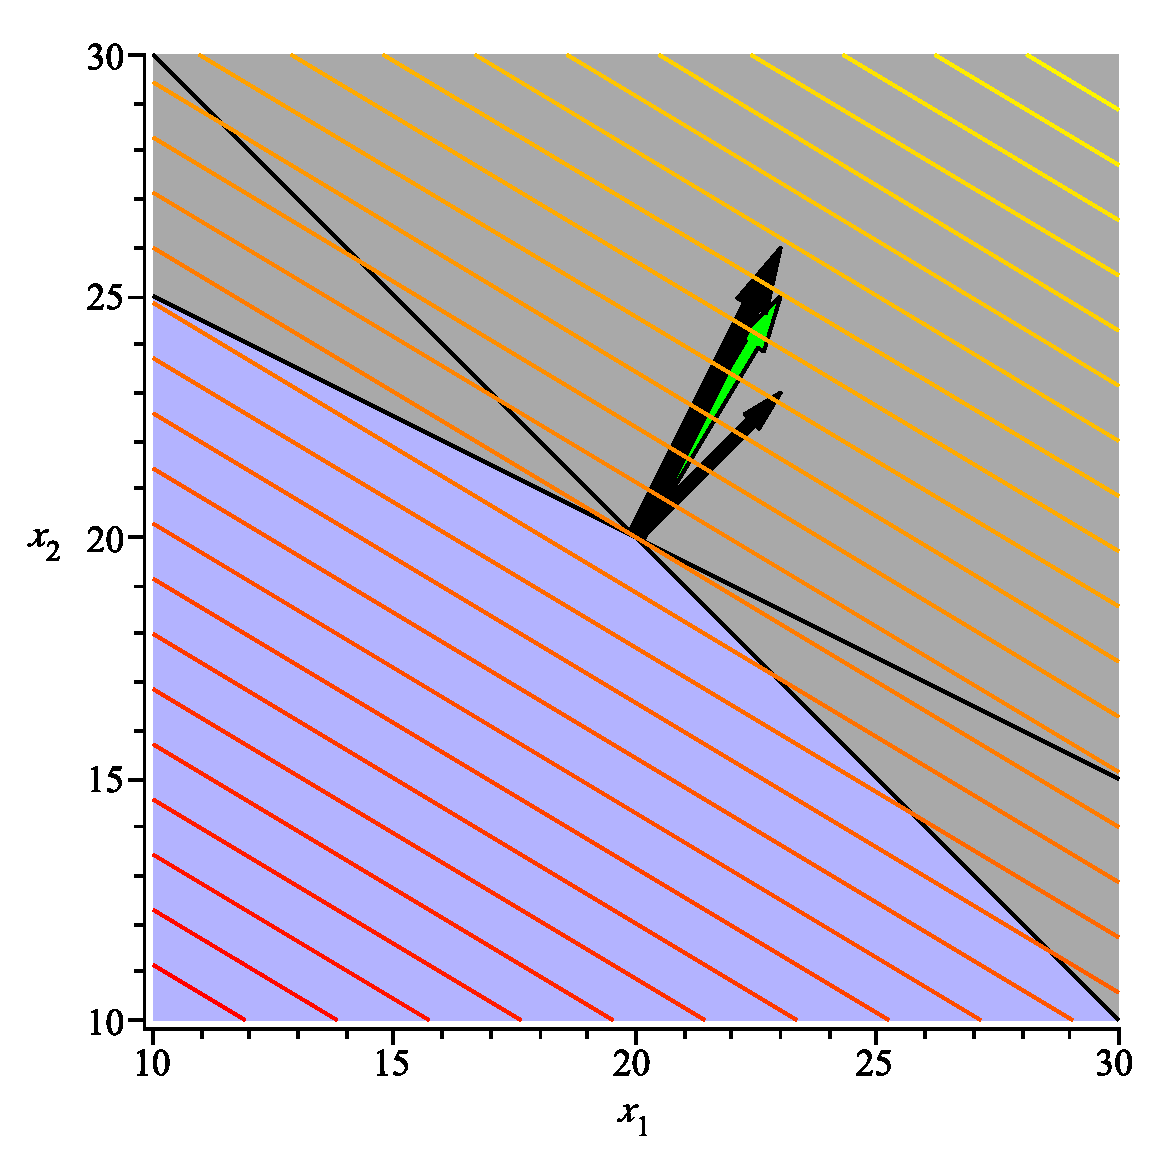
\includegraphics[scale=0.35]{LeatherMakerKKT.pdf}
\caption{This figure illustrates the optimal point of the problem given in Example \ref{ex:KKTSimplex}. Note that at optimality, the objective function gradient is in the dual cone of the binding constraint. That is, it is a positive combination of the gradients of the left-hand-sides of the binding constraints at optimality. The gradient of the objective function is shown in green.}
\label{fig:KKTSimplex}
\end{figure}

We can also verify that the KKT conditions hold for the problem in standard form. Naturally, complementary slackness and primal feasibility hold. To see that dual feasibility holds note that $\mathbf{v} = [0\;\;0\;\;2\;\;1] \geq \mathbf{0}$. Further:
\begin{displaymath}
\begin{bmatrix}2 & 1\end{bmatrix}
\begin{bmatrix} 1 & 2 & 1 & 0\\
1 & 1 & 0 & 1\end{bmatrix} - \begin{bmatrix}
0 & 0 & 2 & 1\end{bmatrix} = \begin{bmatrix} 3 & 5 & 0 & 0\end{bmatrix}
\end{displaymath} 
Here $\begin{bmatrix} 3 & 5 & 0 & 0\end{bmatrix}$ is the objective function coefficient vector for the problem in Standard Form.
\label{ex:KKTSimplex}
\end{example}

\begin{exercise} Use a full simplex tableau to find the values of the Lagrange multipliers (dual variables) at optimality for the problem from Exercise \ref{exer:FindKKT}. Confirm that complementary slackness holds at optimality. Lastly show that dual feasibility holds by showing that the gradient of the objective function ($\mathbf{c}$) is a positive combination of the gradients of the binding constraints at optimality. [Hint: Use the vector $\mathbf{w}$ you should have identified.]
\end{exercise}

\chapter{Duality}
In the last chapter, we explored the Karush-Kuhn-Tucker (KKT) conditions and identified constraints called the \textit{dual feasibility} constraints. In this section, we show that to each linear programming problem (the primal problem) we may associate another linear programming problem (the dual linear programming problem). These two problems are closely related to each other and an analysis of the dual problem can provide deep insight into the primal problem. 


\section{The Dual Problem}
Consider the linear programming problem 
\begin{equation}
P\left\{
\begin{aligned}
\max\;\; & \mathbf{c}^T\mathbf{x}\\
s.t.\;\; & \mathbf{A}\mathbf{x} \leq \mathbf{b}\\
& \mathbf{x} \geq 0
\end{aligned}\right.
\end{equation}

Then the dual problem for Problem $P$ is:
\begin{equation}
D\left\{
\begin{aligned}
\min\;\; & \mathbf{w}\mathbf{b}\\
s.t.\;\; & \mathbf{w}\mathbf{A} \geq \mathbf{c}\\
& \mathbf{w} \geq \mathbf{0}
\end{aligned}\right.
\end{equation}

\begin{remark} Let $\mathbf{v}$ be a vector of \textit{surplus} variables. Then we can transform Problem $D$ into standard form as:
\begin{equation}
D_S\left\{
\begin{aligned}
\min\;\; & \mathbf{w}\mathbf{b}\\
s.t.\;\; & \mathbf{w}\mathbf{A} - \mathbf{v} = \mathbf{c}\\
& \mathbf{w} \geq \mathbf{0}\\
& \mathbf{v} \geq \mathbf{0}
\end{aligned}\right.
\end{equation}
Thus we already see an intimate relationship between duality and the KKT conditions. The feasible region of the dual problem (in standard form) is precisely the the dual feasibility constraints of the KKT conditions for the primal problem.

In this formulation, we see that we have assigned a dual variable $w_i$ ($i=1,\dots,m$) to each constraint in the system of equations $\mathbf{A}\mathbf{x} \leq \mathbf{b}$ of the primal problem. Likewise dual variables $\mathbf{v}$ can be thought of as corresponding to the constraints in $\mathbf{x} \geq \mathbf{0}$. 
\end{remark}

\begin{lemma} The dual of the dual problem is the primal problem.
\label{lem:DualDual}
\end{lemma}
\begin{proof} Rewrite Problem $D$ as:
\begin{equation}
\left\{
\begin{aligned}
\max\;\; & -\mathbf{b}^T\mathbf{w}^T\\
s.t.\;\; & -\mathbf{A}^T\mathbf{w}^T \leq -\mathbf{c}^T\\
& \mathbf{w}^T \geq \mathbf{0}
\end{aligned}\right.
\end{equation}
Let $\boldsymbol{\beta} = -\mathbf{b}^T$, $\mathbf{G} = -\mathbf{A}^T$, $\mathbf{u} = \mathbf{w}^T$ and $\boldsymbol{\kappa} = -\mathbf{c}^T$. Then this new problem becomes:
\begin{equation}
\left\{
\begin{aligned}
\max\;\; & \boldsymbol{\beta}\mathbf{u}\\
s.t.\;\; & \mathbf{G}\mathbf{u} \leq \boldsymbol{\kappa}\\
& \mathbf{u} \geq \mathbf{0}
\end{aligned}\right.
\end{equation}
Let $\mathbf{x}^T$ be the vector of dual variables (transposed) for this problem. We can formulate the dual problem as:
\begin{equation}
\left\{
\begin{aligned}
\min\;\; & \mathbf{x}^T\boldsymbol{\kappa}\\
s.t.\;\; & \mathbf{x}^T\mathbf{G} \geq \boldsymbol{\beta}\\
& \mathbf{x}^T \geq \mathbf{0}
\end{aligned}\right.
\end{equation}
Expanding, this becomes:
\begin{equation}
\left\{
\begin{aligned}
\min\;\; & -\mathbf{x}^T\mathbf{c}^T\\
s.t.\;\; & -\mathbf{x}^T\mathbf{A}^T \geq -\mathbf{b}^T\\
& \mathbf{x}^T \geq \mathbf{0}
\end{aligned}\right.
\end{equation}
This can be simplified to:
\begin{equation}
P\left\{
\begin{aligned}
\max\;\; & \mathbf{c}^T\mathbf{x}\\
s.t.\;\; & \mathbf{A}\mathbf{x} \leq \mathbf{b}\\
& \mathbf{x} \geq 0
\end{aligned}\right.
\end{equation}
as required. This completes the proof.
\end{proof}

Lemma \ref{lem:DualDual} shows that the notion of dual and primal can be exchanged and that it is simply a matter of perspective which problem is the dual problem and which is the primal problem. Likewise, by transforming problems into canonical form, we can develop dual problems for any linear programming problem. 

The process of developing these formulations can be exceptionally tedious, as it requires enumeration of all the possible combinations of various linear and variable constraints. The following table summarizes the process of converting an arbitrary primal problem into its dual. This table can be found in Chapter 6 of \cite{BJS04}.

\begin{table}[hbt]
\centering
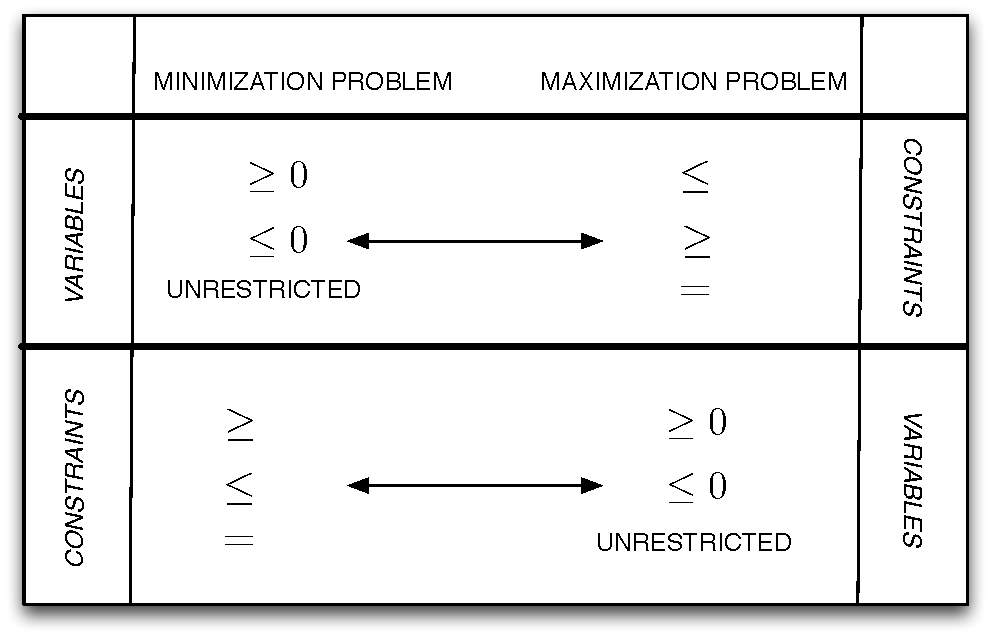
\includegraphics[scale=0.5]{DualConversionTable.pdf}
\caption{Table of Dual Conversions: To create a dual problem, assign a dual variable to each constraint of the form $\mathbf{A}\mathbf{x} \circ \mathbf{b}$, where $\circ$ represents a binary relation. Then use the table to determine the appropriate sign of the inequality in the dual problem as well as the nature of the dual variables.}
\label{tab:Duality}
\end{table}

\begin{example} Consider the problem of finding the dual problem for the Toy Maker Problem (Example \ref{ex:ToyMaker}) in standard form. The primal problem is:
\begin{displaymath}
\begin{aligned}
\max\;\;&7x_1 + 6x_2\\
s.t.\;\;& 3x_1 + x_2 + s_1 = 120\quad & (w_1)\\
& x_1 + 2x_2 + s_2 = 160\quad & (w_2)\\
&x_1 + s_3 = 35\quad & (w_3)\\
&x_1, x_2, s_1, s_2, s_3 \geq 0
\end{aligned}
\end{displaymath}
Here we have placed dual variable names ($w_1$, $w_2$ and $w_3$) next to the constraints to which they correspond. 

The primal problem variables in this case are all positive, so using Table \ref{tab:Duality} we know that the constraints of the dual problem will be greater-than-or-equal-to constraints. Likewise, we know that the dual variables will be unrestricted in sign since the primal problem constraints are all equality constraints.

The coefficient matrix is:
\begin{displaymath}
\mathbf{A} = 
\begin{bmatrix}
3 & 1 & 1 & 0 & 0\\
1 & 2 & 0 & 1 & 0\\
1 & 0 & 0 & 0 & 1
\end{bmatrix}
\end{displaymath}
Clearly we have:
\begin{gather*}
\mathbf{c} = \begin{bmatrix}7 & 6 & 0 & 0 & 0\end{bmatrix}\\
\mathbf{b}= \begin{bmatrix}120 \\160 \\ 35\end{bmatrix}
\end{gather*} 
Since $\mathbf{w} = [w_1 \;\; w_2 \;\; w_3]$, we know that $\mathbf{w}\mathbf{A}$ will be:
\begin{displaymath}
\mathbf{w}\mathbf{A} = 
\begin{bmatrix}
3w_1 + w_2 + w_3 & w_1 + 2w_2 & w_1 & w_2 & w_3
\end{bmatrix}
\end{displaymath}
This vector will be related to $\mathbf{c}$ in the constraints of the dual problem. \textbf{Remember, in this case, all constraints are greater-than-or-equal-to}. Thus we see that the constraints of the dual problem are:
\begin{align*}
3w_1 + w_2 + w_3 \geq 7\\
w_1 + 2w_2 \geq 6\\
w_1 \geq 0\\
w_2 \geq 0\\
w_3 \geq 0 
\end{align*}

We also have the redundant set of constraints that tell us $\mathbf{w}$ is unrestricted because the primal problem had equality constraints. This \textit{will always} happen in cases when  you've introduced slack variables into a problem to put it in standard form. This should be clear from the definition of the dual problem for a maximization problem in canonical form. 

Thus the whole dual problem becomes:
\begin{equation}
\begin{aligned}
\min\;\;&120w_1 + 160w_2 + 35w_3\\
s.t.\;\; & 3w_1 + w_2 + w_3 \geq 7\\
&w_1 + 2w_2 \geq 6\\
&w_1 \geq 0\\
&w_2 \geq 0\\
&w_3 \geq 0 \\
&\mathbf{w}\quad\text{unrestricted}
\end{aligned}
\end{equation}

Again, note that in reality, the constraints we derived from the $\mathbf{w}\mathbf{A}\geq\mathbf{c}$ part of the dual problem make the constraints ``$\mathbf{w}$ unrestricted'' redundant, for in fact $\mathbf{w} \geq \mathbf{0}$ just as we would expect it to be if we'd found the dual of the Toy Maker problem given in canonical form.
\end{example}


\begin{exercise} Identify the dual problem for:
\begin{displaymath}
\begin{aligned}
\max\;\;&x_1 + x_2\\
s.t.\;\;&2x_1 + x_2 \geq 4\\
&x_1 + 2x_2 \leq 6\\
&x_1, x_2 \geq 0
\end{aligned}
\end{displaymath}
\end{exercise}

\begin{exercise} Use the table or the definition of duality to determine the dual for the problem:
\begin{equation}
\left\{
\begin{aligned}
\min\;\; & \mathbf{c}\mathbf{x}\\
s.t.\;\; & \mathbf{A}\mathbf{x} \leq \mathbf{b}\\
& \mathbf{x} \geq 0
\end{aligned}\right.
\end{equation}
Compare it to the KKT conditions you derived in Exercise \ref{exer:MinKKT}.
\end{exercise}

\section{Weak Duality}
There is a deep relationship between the objective function value, feasibility and boundedness of the primal problem and the dual problem. We will explore these relationships in the following lemmas.

\begin{lemma}[Weak Duality] For the primal problem $P$ and dual problem $D$ let $\mathbf{x}$ and $\mathbf{w}$ be feasible solutions to Problem $P$ and Problem $D$ respectively. Then:
\begin{equation}
\mathbf{w}\mathbf{b} \geq \mathbf{c}\mathbf{x}
\label{eqn:WeakDual0}
\end{equation}
\label{lem:WeakDuality}
\end{lemma}
\begin{proof} Primal feasibility ensures that:
\begin{displaymath}
\mathbf{A}\mathbf{x} \leq \mathbf{b}
\end{displaymath}
Therefore, we have:
\begin{equation}
\mathbf{w}\mathbf{A}\mathbf{x} \leq \mathbf{w}\mathbf{b}
\label{eqn:WeakDual1}
\end{equation}

Dual feasibility ensure that:
\begin{displaymath}
\mathbf{w}\mathbf{A} \geq \mathbf{c}
\end{displaymath}
Therefore we have:
\begin{equation}
\mathbf{w}\mathbf{A}\mathbf{x} \geq \mathbf{c}\mathbf{x}
\label{eqn:WeakDual2}
\end{equation}

Combining Equations \ref{eqn:WeakDual1} and \ref{eqn:WeakDual2} yields Equation \ref{eqn:WeakDual0}:
\begin{displaymath}
\mathbf{w}\mathbf{b} \geq \mathbf{c}\mathbf{x}
\end{displaymath}
This completes the proof.
\end{proof}

\begin{remark}
Lemma \ref{lem:WeakDuality} ensures that the optimal solution $\mathbf{w}^*$ for Problem $D$ must provide an \textit{upper bound} to Problem $P$, since for any feasible $\mathbf{x}$, we know that:
\begin{equation}
\mathbf{w}^*\mathbf{b} \geq \mathbf{c}\mathbf{x}
\end{equation}
Likewise, any optimal solution to Problem $P$ provides a lower bound on solution $D$. 
\end{remark}

\begin{corollary} If Problem $P$ is unbounded, then Problem $D$ is infeasible. Likewise, if Problem $D$ is unbounded, then Problem $P$ is infeasible.
\label{cor:WeakDuality2}
\end{corollary} 
\begin{proof} For any $\mathbf{x}$, feasible to Problem $P$ we know  that $\mathbf{w}\mathbf{b} \geq \mathbf{c}\mathbf{x}$ for any feasible $\mathbf{w}$. The fact that Problem $P$ is unbounded implies that for any $V \in \mathbb{R}$ we can find an $\mathbf{x}$ feasible to Problem $P$ that $\mathbf{c}\mathbf{x} > V$. If $\mathbf{w}$ were feasible to Problem $D$, then we would have $\mathbf{w}\mathbf{b} > V$ for any arbitrarily chosen $V$. There can be no finite vector $\mathbf{w}$ with this property and we conclude that Problem $D$ must be infeasible. 

The alternative case that when Problem $D$ is unbounded, then Problem $P$ is infeasible follows by reversing the roles of the problem. This completes the proof.
\end{proof}

\section{Strong Duality}
\begin{lemma} Problem $D$ has an optimal solution $\mathbf{w}^* \in \mathbb{R}^m$ if and only if there exists vector $\mathbf{x}^* \in \mathbb{R}^n$ and $\mathbf{s}^* \in \mathbb{R}^m$ such that:
\begin{align}
\text{Primal Feasibility}&\left\{ 
\begin{aligned}
\mathbf{w}^*\mathbf{A} \geq \mathbf{c}\\
\mathbf{w}^* \geq 0
\label{eqn:KKTDual1}
\end{aligned}\right.\\
\text{Dual Feasibility}&\left\{ 
\begin{aligned}
\mathbf{A}\mathbf{x}^* + \mathbf{s}^* = \mathbf{b}\\
\mathbf{x}^* \geq 0\\
\mathbf{s}^* \geq 0
\label{eqn:KKTDual2}
\end{aligned}\right.\\
\text{Complementary Slackness}&\left\{ 
\begin{aligned}
\left(\mathbf{w}^*\mathbf{A} - \mathbf{c}\right)\mathbf{x}^* = 0\\
\mathbf{w}^*\mathbf{s}^* = 0
\label{eqn:KKTDual3}
\end{aligned}\right.
\end{align}
Furthermore, these KKT conditions are equivalent to the KKT conditions for the primal problem.
\label{lem:DualKKT}
\end{lemma}
\begin{proof} Following the proof of Lemma \ref{lem:DualDual}, let $\boldsymbol{\beta} = -\mathbf{b}^T$, $\mathbf{G} = -\mathbf{A}^T$, $\mathbf{u} = \mathbf{w}^T$ and $\boldsymbol{\kappa} = -\mathbf{c}^T$. Then the dual problem can be rewritten as:
\begin{displaymath}
\left\{
\begin{aligned}
\max\;\; & \boldsymbol{\beta}\mathbf{u}\\
s.t.\;\; & \mathbf{G}\mathbf{u} \leq \boldsymbol{\kappa}\\
& \mathbf{u} \geq \mathbf{0}
\end{aligned}\right.
\end{displaymath}
Let $\mathbf{x}^T \in \mathbb{R}^{1 \times n}$ and $s^T \in \mathbb{R}^{1 \times m}$ be the dual variables for this problem. Then applying Theorem \ref{thm:KKT}, we obtain KKT conditions for this problem:
\begin{align}
\text{Primal Feasibility}&\left\{ 
\begin{aligned}
\mathbf{G}\mathbf{u}^* \leq \boldsymbol{\kappa}\\
\mathbf{u}^* \geq \mathbf{0}
\end{aligned}\right.\\
\text{Dual Feasibility}&\left\{ 
\begin{aligned}
{\mathbf{x}^*}^T\mathbf{G} - {\mathbf{s}^*}^T = \boldsymbol{\beta}\\
{\mathbf{x}^*}^T \geq \mathbf{0}\\
{\mathbf{s}^*}^T \geq \mathbf{0}
\end{aligned}\right.\\
\text{Complementary Slackness}&\left\{ 
\begin{aligned}
{\mathbf{x}^*}^T\left(\mathbf{G}\mathbf{u}^* - \boldsymbol{\kappa}\right) = 0\\
{\mathbf{s}^*}^T\mathbf{u}^* = 0
\end{aligned}\right.
\end{align}
We can rewrite:
\begin{gather*}
\mathbf{G}\mathbf{u}^* \leq \boldsymbol{\kappa} \equiv -\mathbf{A}^T\mathbf{w}^T \leq -\mathbf{c}^T \equiv \mathbf{w}\mathbf{A} \geq \mathbf{c}\\
{\mathbf{x}^*}^T\mathbf{G} - {\mathbf{s}^*}^T = \boldsymbol{\beta} \equiv
{\mathbf{x}^*}^T(-\mathbf{A}^T) - {\mathbf{s}^*}^T = -\mathbf{b}^T \equiv
\mathbf{A}\mathbf{x}^* + \mathbf{s}^* = \mathbf{b}\\
{\mathbf{x}^*}^T\left(\mathbf{G}\mathbf{u}^* - \boldsymbol{\kappa}\right) = 0 \equiv
{\mathbf{x}^*}^T\left((-\mathbf{A}^T){\mathbf{w}^*}^T - (-\mathbf{c}^T)\right) = 0 \equiv (\mathbf{w}^*\mathbf{A} - \mathbf{c})\mathbf{x}^* = 0\\
{\mathbf{s}^*}^T\mathbf{u}^* = 0 \equiv {\mathbf{s}^*}^T{\mathbf{w}^*}^T = 0 \equiv \mathbf{w}^*\mathbf{s}^* = 0
\end{gather*}
Thus, we have shown that the KKT conditions for the dual problem are:
\begin{align*}
\text{Primal Feasibility}&\left\{ 
\begin{aligned}
\mathbf{w}^*\mathbf{A} \geq \mathbf{c}\\
\mathbf{w}^* \geq 0
\end{aligned}\right.\\
\text{Dual Feasibility}&\left\{ 
\begin{aligned}
\mathbf{A}\mathbf{x}^* + \mathbf{s}^* = \mathbf{b}\\
\mathbf{x}^* \geq 0\\
\mathbf{s}^* \geq 0
\end{aligned}\right.\\
\text{Complementary Slackness}&\left\{ 
\begin{aligned}
\left(\mathbf{w}^*\mathbf{A} - \mathbf{c}\right)\mathbf{x}^* = 0\\
\mathbf{w}^*\mathbf{s}^* = 0
\end{aligned}\right.
\end{align*}

To prove the equivalence to the KKT conditions for the primal problem, define:
\begin{gather}
\mathbf{s}^* = \mathbf{b} - \mathbf{A}\mathbf{x}^* \\
\mathbf{v}^* = \mathbf{w}^*\mathbf{A} - \mathbf{c}
\end{gather}
That is, $\mathbf{s}^*$ is a vector slack variables for the primal problem $P$ at optimality and $\mathbf{v}^*$ is a vector of surplus variables for the dual problem $D$ at optimality. Recall the KKT conditions for the primal problem are:
\begin{align*}
\text{Primal Feasibility}&\left\{ 
\begin{aligned}
\mathbf{A}\mathbf{x}^* \leq \mathbf{b}\\
\mathbf{x}^* \geq \mathbf{0}
\end{aligned}\right.\\
\text{Dual Feasibility}&\left\{ 
\begin{aligned}
\mathbf{w}^*\mathbf{A} - \mathbf{v}^* = \mathbf{c}\\
\mathbf{w}^* \geq \mathbf{0}\\
\mathbf{v}^* \geq \mathbf{0}
\end{aligned}\right.\\
\text{Complementary Slackness}&\left\{ 
\begin{aligned}
\mathbf{w}^*\left(\mathbf{A}\mathbf{x}^* - \mathbf{b}\right) = 0\\
\mathbf{v}^*\mathbf{x}^* = 0
\end{aligned}\right.
\end{align*}

We can rewrite these as:
\begin{align}
\text{Primal Feasibility}&\left\{ 
\begin{aligned}
\mathbf{A}\mathbf{x}^* + \mathbf{s}^* = \mathbf{b}\\
\mathbf{x}^* \geq \mathbf{0}
\end{aligned}\right.\\
\text{Dual Feasibility}&\left\{ 
\begin{aligned}
\mathbf{w}^*\mathbf{A} - \mathbf{v}^* = \mathbf{c}\\
\mathbf{w}^* \geq \mathbf{0}\\
\mathbf{v}^* \geq \mathbf{0}
\end{aligned}\right.\\
\text{Complementary Slackness}&\left\{ 
\begin{aligned}
\mathbf{w}^*\left(\mathbf{s}^*\right) = 0\\
\mathbf{v}^*\mathbf{x}^* = 0
\end{aligned}\right.
\end{align}
Where the complementary slackness condition $\mathbf{w}^*(\mathbf{A}\mathbf{x}^* - \mathbf{b}) = 0$ is re-written as:
\begin{displaymath}
\mathbf{w}^*(\mathbf{A}\mathbf{x}^* - \mathbf{b}) = 0 \equiv \mathbf{w}^*(-(\mathbf{b} - \mathbf{A}\mathbf{x}^*) = 0 \equiv \mathbf{w}^*(-\mathbf{s}^*) = 0 \equiv \mathbf{w}^*(\mathbf{s}^*) 
\end{displaymath}

Likewise beginning with the KKT conditions for the dual problem (Expression \ref{eqn:KKTDual1} - \ref{eqn:KKTDual3}) we can write:
\begin{align*}
\text{Primal Feasibility}&\left\{ 
\begin{aligned}
\mathbf{w}^*\mathbf{A} - \mathbf{v}^* \geq \mathbf{c}\\
\mathbf{w}^* \geq 0
\end{aligned}\right.\\
\text{Dual Feasibility}&\left\{ 
\begin{aligned}
\mathbf{A}\mathbf{x}^* + \mathbf{s}^* = \mathbf{b}\\
\mathbf{x}^* \geq 0\\
\mathbf{s}^* \geq 0
\end{aligned}\right.\\
\text{Complementary Slackness}&\left\{ 
\begin{aligned}
\left(\mathbf{v}^*\right)\mathbf{x}^* = 0\\
\mathbf{w}^*\mathbf{s}^* = 0
\end{aligned}\right.
\end{align*}
Here we substitute $\mathbf{v}^*$ for $\mathbf{w}^*\mathbf{A} - \mathbf{c}$ in the complementary slackness terms. Thus we can see that the KKT conditions for the primal and dual problems are equivalent. This completes the proof.
\end{proof}
\begin{remark} Notice that the KKT conditions for the primal and dual problems are equivalent, but the dual feasibility conditions for the primal problem are identical to the primal feasibility conditions for the dual problem and vice-versa. Thus, two linear programming problems are dual to each other if they share KKT conditions with the primal and dual feasibility conditions swapped.
\end{remark}


\begin{exercise} Compute the dual problem for a canonical form minimization problem:
\begin{displaymath}
P\left\{
\begin{aligned}
\min\;\;&\mathbf{c}\mathbf{x}\\
s.t.\;\;&\mathbf{A}\mathbf{x} \geq \mathbf{b}\\
& \mathbf{x} \geq \mathbf{0}
\end{aligned}\right.
\end{displaymath}
Find the KKT conditions for the dual problem you just identified. Use the result from Exercise \ref{exer:MinKKT} to show that KKT conditions for Problem $P$ are identical to the KKT conditions for the dual problem you just found.
\end{exercise}
%\begin{exercise} Prove Lemma \ref{lem:DualKKT}. [Hint: Transform Problem $D$ into a canonical form maximization problem and find the KKT conditions where the dual variables are $\mathbf{x}^*$ and $\mathbf{s}^*$. Then simplify the KKT conditions to obtain those stated in the formula. To prove equivalence, let $\mathbf{v} = \mathbf{w}\mathbf{A} - \mathbf{c}$ with $\mathbf{v} \geq \mathbf{0}$. Argue that $\mathbf{A}\mathbf{x}^* + \mathbf{s}^* = \mathbf{b}$, $\mathbf{x}^*,\mathbf{s}^* \geq \mathbf{0}$ implies that $\mathbf{x}^*$ is feasible to the primal problem. Then show that by subtituting in $\mathbf{v}^*$ for $\mathbf{w}^*\mathbf{A} - \mathbf{c}$ and $\mathbf{s}^* = \mathbf{b}-\mathbf{A}\mathbf{x}^*$ that the complementary slackness conditions for both problems are identical.]
%\end{exercise}

\begin{lemma}[Strong Duality] There is a bounded optimal solution $\mathbf{x}^*$ for Problem $P$ if and only if there is a bounded optimal solution $\mathbf{w}^*$ for Problem $D$. Furthermore, $\mathbf{c}\mathbf{x}^* = \mathbf{w}^*\mathbf{b}$.
\label{lem:StrongDuality}
\end{lemma}
\begin{proof} Suppose that there is a solution $\mathbf{x}^*$ for Problem $P$. Let $\mathbf{s}^* = \mathbf{b} - \mathbf{A}\mathbf{x}^*$. Clearly $\mathbf{s}^* \geq \mathbf{0}$. 

By Theorem \ref{thm:KKT} there exists dual variables $\mathbf{w}^*$ and $\mathbf{v}^*$ satisfying dual feasibility and complementary slackness. Dual feasibility in the KKT conditions implies that:
\begin{equation}
\mathbf{v}^* = \mathbf{w}^*\mathbf{A} - \mathbf{c}
\end{equation}
We also know that $\mathbf{w}^*,\mathbf{v}^* \geq \mathbf{0}$. Complementary Slackness (from Theorem \ref{thm:KKT}) states that $\mathbf{v}^*\mathbf{x}^* = 0$. But $\mathbf{v}^*$ is defined above and we see that: 
\begin{equation}
\mathbf{v}^*\mathbf{x}^* = 0 \implies \left(\mathbf{w}^*\mathbf{A} - \mathbf{c}\right)\mathbf{x} = 0
\end{equation}

Likewise, since we have $\mathbf{s}^* = \mathbf{b} - \mathbf{A}\mathbf{x}^*$. Complementary slackness assures us that $\mathbf{w}^*\left(\mathbf{b} - \mathbf{A}\mathbf{x}^*\right) = 0$. Thus we see that:
\begin{equation}
\mathbf{w}^*\left(\mathbf{b} - \mathbf{A}\mathbf{x}^*\right) = 0 \implies \mathbf{w}^*\mathbf{s}^* = 0
\end{equation}
Thus it follows from Lemma  \ref{lem:DualKKT} that $\mathbf{w}^*$ is an optimal solution to Problem $D$ since it satisfies the KKT conditions. The fact that Problem $P$ has an optimal solution when Problem $D$ has an optimal solution can be proved in a similar manner starting with the KKT conditions given in Lemma \ref{lem:DualKKT} and applying the same reasoning as above. 

Finally, at optimality, we know from Lemma \ref{lem:DualKKT} that:
\begin{equation}
\left(\mathbf{w}^*\mathbf{A} - \mathbf{c}\right)\mathbf{x}^* = 0 \implies \mathbf{w}^*\mathbf{A}\mathbf{x}^* = \mathbf{c}\mathbf{x}^*
\end{equation}
We also know from Theorem \ref{thm:KKT} that:
\begin{equation}
\mathbf{w}^*\left(\mathbf{b} - \mathbf{A}\mathbf{x}^*\right) = 0\implies  \mathbf{w}^*\mathbf{b} = \mathbf{w}^*\mathbf{A}\mathbf{x}^*
\end{equation}
Therefore we have: $\mathbf{w}^*\mathbf{b} = \mathbf{c}\mathbf{x}^*$. This completes the proof.
\end{proof}

\begin{corollary} If Problem $P$ is infeasible, then Problem $D$ is either unbounded or infeasible. If Problem $D$ is infeasible, then either Problem $P$ is unbounded or infeasible.
\label{cor:DualInfeas}
\end{corollary}
\begin{proof} This result follows by contrapositive from Lemma \ref{lem:StrongDuality}. To see this, suppose that Problem $P$ is infeasible. Then Problem $P$ has no bounded optimal solution. Therefore, Problem $D$ has no bounded optimal solution (by Lemma \ref{lem:StrongDuality}). If Problem $D$ has no bounded optimal solution, then either Problem $D$ is unbounded or it is infeasible. A symmetric argument on Problem $D$ completes the proof of the Lemma. 
\end{proof}

\begin{exercise} Consider the problem 
\begin{displaymath}
\begin{aligned}
\max\;\;&x_1 + x_2\\
s.t.\;\;&x_1 - x_2 \geq 1\\
& -x_1 + x_2 \geq 1\\
&x_1,x_2 \geq 0
\end{aligned}
\end{displaymath}
\begin{enumerate}
\item Show that this problem is infeasible. 
\item Compute its dual. 
\item Show that the dual is infeasible, thus illustrating Corollary \ref{cor:DualInfeas}.
\end{enumerate}
\end{exercise}

The following theorem summarizes all of the results we have obtained in the last two sections.
\begin{theorem}[Strong Duality Theorem] Consider Problem $P$ and Problem $D$. Then exactly one of the following statements is true:
\begin{enumerate*}
\item Both Problem $P$ and Problem $D$ possess optimal solutions $\mathbf{x}^*$ and $\mathbf{w}^*$ respectively and $\mathbf{c}\mathbf{x}^* = \mathbf{w}^*\mathbf{b}$.
\item Problem $P$ is unbounded and Problem $D$ is infeasible.
\item Problem $D$ is unbounded and Problem $P$ is infeasible.
\item Both problems are infeasible.
\end{enumerate*}
\label{thm:StrongDuality}
\end{theorem}

\section{Geometry of the Dual Problem}
The geometry of the dual problem is, in essence, exactly the same the geometry of the primal problem insofar as they are both linear programming problems and thus their feasible regions are polyhedral sets\footnote{Thanks for Michael Cline for suggesting this section.}. Certain examples have a very nice geometric visualization. Consider the problem:
\begin{equation}
\left\{
\begin{aligned}
\max\;\; & 6x_1 + 6x_2 \\
s.t.\;\; & 3x_1 + 2x_2 \leq 6\\
 & 2x_1 + 3x_2 \leq 6\\
 & x_1, x_2 \geq 0
\end{aligned}\right.
\label{eqn:SymmetricDual}
\end{equation}
In this problem we have:
\begin{displaymath}
\mathbf{A} = \begin{bmatrix}3 & 2\\2 & 3\end{bmatrix}\quad \mathbf{c} = \begin{bmatrix}6 & 6\end{bmatrix} \quad \mathbf{b} = \begin{bmatrix}6\\6\end{bmatrix}
\end{displaymath}
Notice that $\mathbf{A}$ is a symmetric matrix and $\mathbf{c}^T = \mathbf{b}$ and the dual problem is:
\begin{equation}
\left\{
\begin{aligned}
\min \;\; & 6w_1 + 6w_2 \\
s.t.\;\; & 3w_1 + 2w_2 \geq 6\\
 & 2w_1 + 3w_2 \leq 6\\
 & w_1, w_2 \geq 0
\end{aligned}\right.
\label{eqn:SymmetricDual}
\end{equation}
This results in a geometry in which the dual feasible region is a reflection of the primal feasible region (ignoring non-negativity constraints). This is illustrated in Figure \ref{fig:PrimalDualFeasibleRegion-1}.
\begin{figure}[htbp]
\centering
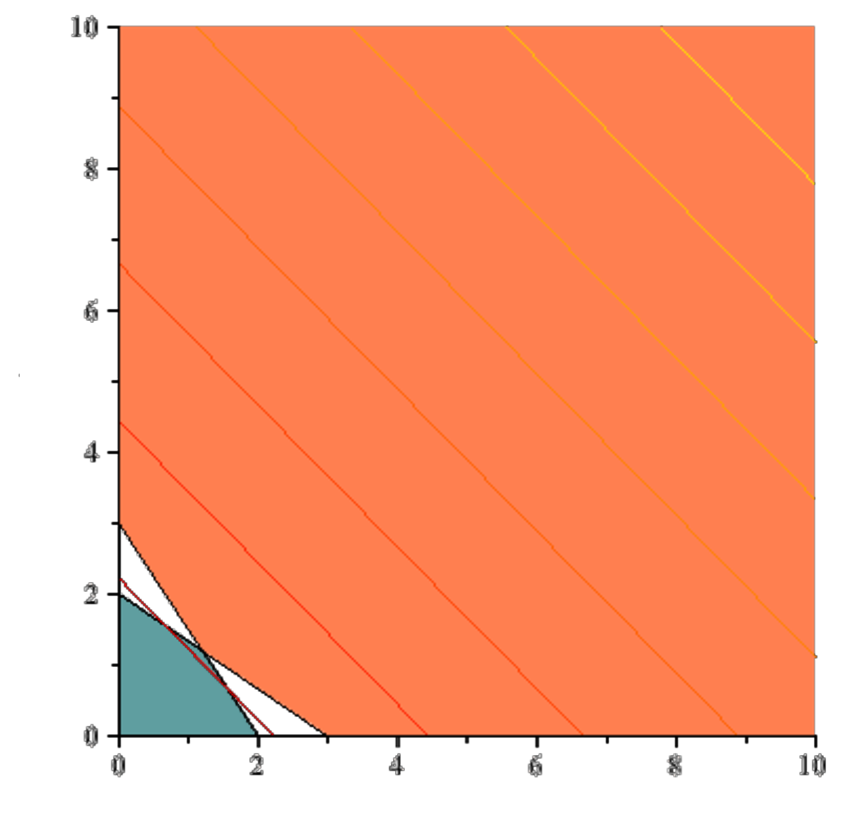
\includegraphics[scale=0.5]{PrimalDualFeasibleRegion-1.pdf}
\caption{The dual feasible region in this problem is a mirror image (almost) of the primal feasible region. This occurs when the right-hand-side vector $\mathbf{b}$ is equal to the objective function coefficient column vector $\mathbf{c}^T$ and the matrix $\mathbf{A}$ is symmetric.}
\label{fig:PrimalDualFeasibleRegion-1} 
\end{figure}

We can also illustrate the process of solving this problem using the (revised) simplex algorithm. In doing so, we first convert Problem \ref{eqn:SymmetricDual} to standard form:
\begin{equation}
\left\{
\begin{aligned}
\max\;\; & 6x_1 + 6x_2 \\
s.t.\;\; & 3x_1 + 2x_2 + s_1 \phantom{+s_2}= 6\\
 & 2x_1 + 3x_2 \phantom{+s_1} + s_2 = 6\\
 & x_1, x_2 \geq 0
\end{aligned}\right.
\label{eqn:SymmetricDual}
\end{equation}
This yields an initial tableau:
\begin{equation}
\begin{array}{c}
z\\
s_1\\
s_2
\end{array}
\left[
\begin{array}{cc|c}
0	&	0	&	0\\
\hline
1	&	0	&   6\\
0	&	1	&	6
\end{array}
\right]
\end{equation}
This is because our initial $\mathbf{c}_\mathbf{B} = \begin{bmatrix}0&0\end{bmatrix}$ and thus $\mathbf{w} = \begin{bmatrix}0&0\end{bmatrix}$. This means at the start of the simplex algorithm, $w_1 = 0$ and $w_2 = 0$ and $x_1 = 0$ and $x_2 = 0$, so we begin at the origin, which is \textbf{in the primal feasible region} and \textbf{not in the dual feasible region}. If we iterate and choose $x_1$ as an entering variable, our updated tableau will be:
\begin{equation}
\begin{array}{c}
z\\
x_1\\
s_2
\end{array}
\left[
\begin{array}{cc|c}
2	&	0	&	12\\
\hline
1/3	&	0	&   2\\
-2/3	&	1	&	2
\end{array}
\right]
\end{equation}
Notice at this point, $x_1 = 2$, $x_2 = 0$ and $w_1 = 2$ and $w_2 = 0$. This point is again feasible for the primal problem but still infeasible for the dual. This step is illustrated in Figure \ref{fig:PrimalDualFeasibleRegion-2}. Entering $x_2$ yields the final tableau:
\begin{equation}
\begin{array}{c}
z\\
x_1\\
x_2
\end{array}
\left[
\begin{array}{cc|c}
6/5	&	6/5	&	72/5\\
\hline
3/5	&	-2/5	&   6/5\\
-2/5	&	3/5	&	6/5
\end{array}
\right]
\end{equation}
At this final point, $x_1 = x_2 = w_1 = w_2 = \tfrac{6}{5}$, which is feasible to both problems. This step is also illustrated in Figure \ref{fig:PrimalDualFeasibleRegion-2}.
\begin{figure}[htbp]
\centering
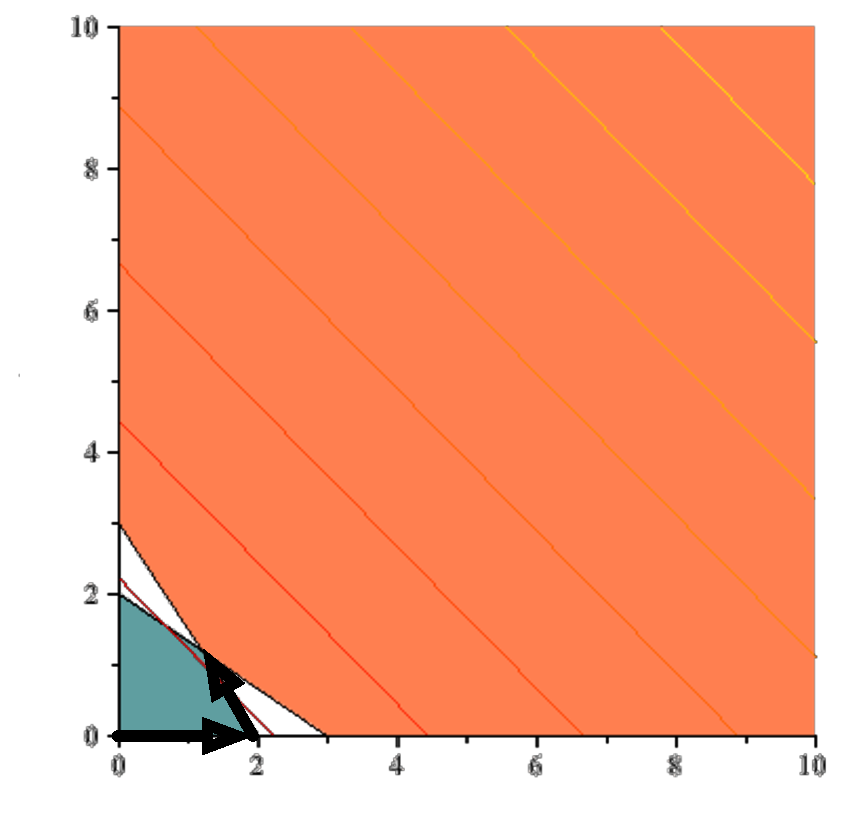
\includegraphics[scale=0.5]{PrimalDualFeasibleRegion-2.pdf}
\caption{The simplex algorithm begins at a feasible point in the feasible region of the primal problem. In this case, this is also the same starting point in the dual problem, which is infeasible. The simplex algorithm moves through the feasible region of the primal problem towards a point in the dual feasible region. At the conclusion of the algorithm, the algorithm reaches the unique point that is both primal and dual feasible.}
\label{fig:PrimalDualFeasibleRegion-2} 
\end{figure}
We should note that this problem is atypical in that the primal and dual feasible regions share one common point. In more standard problems, the two feasible regions cannot be drawn in this convenient way, \textit{but} the simplex process is the same. The simplex algorithm begins at a point in the primal feasible region with a corresponding dual vector that is \textit{not} in the feasible region of the dual problem. As the simplex algorithm progresses, this dual vector approaches and finally enters the dual feasible region.

\begin{exercise} Draw the dual feasible region for the following problem.
\begin{displaymath}
\begin{aligned}
\max\;\; & 3x_1 + 5x_2\\
s.t.\;\; & x_1 + 2x_2 \leq 60\\
& x_1 + x_2 \leq 40\\
& x_1, x_2 \geq 0
\end{aligned}
\end{displaymath}
Solve the problem using the revised simplex algorithm and trace the path of dual variables (the $\mathbf{w}$ vector) in your plot of the dual feasible region. Also trace the path of the primal vector $\mathbf{x}$ through the primal feasible region. [Hint: Be sure to draw the area around the dual feasible region. Your dual vector $\mathbf{w}$ will not enter the feasible region until the last simplex pivot.]
\end{exercise}

\section{Economic Interpretation of the Dual Problem}
Consider again, the value of the objective function in terms of the values of the non-basic variables (Equation \ref{eqn:Obj2}):
\begin{equation}
z=\mathbf{c}\mathbf{x} = 
\mathbf{c_B}\mathbf{B}^{-1}\mathbf{b} + 
\left(\mathbf{c_N} - \mathbf{c_B}\mathbf{B}^{-1}\mathbf{N}\right)\mathbf{x}_N
\end{equation}
Suppose we are at a non-degenerate optimal point. We've already observed that:
\begin{equation}
\frac{\partial z}{\partial x_j} = -(z_j - c_j) = c_j - \mathbf{c}_\mathbf{B}\mathbf{B}^{-1}\mathbf{A}_{\cdot j}
\end{equation}
We can rewrite all these equations in terms of our newly defined term:
\begin{equation}
\mathbf{w} = \mathbf{c}_{\mathbf{B}}\mathbf{B}^{-1}
\end{equation}
to obtain:
\begin{equation}
z = \mathbf{w}\mathbf{b} + 
\left(\mathbf{c_N} - \mathbf{w}\mathbf{N}\right)\mathbf{x}_N
\end{equation}
Remember, $\mathbf{w}$ is the vector of dual variables corresponding to the constraints in our original problem $P$.
 
Suppose we fix the values of $\mathbf{x}_{\mathbf{N}}$. Then we can see that the vector $\mathbf{w}$ has individual elements with the property that:
\begin{equation}
\frac{\partial z}{\partial b_i} = w_i 
\end{equation}
That is, the $i^\text{th}$ element of $\mathbf{w}$ represents the amount that the objective function value would change at optimality assuming we could modify the right-hand-side of the constraints. \textbf{Note, this result holds only in the absence of degeneracy, for reasons we will see in an example.}

Thus, we can think of $w_i$ as the \textit{shadow price} for resource $i$ (the right-hand-side of the $i^\text{th}$ constraint). A shadow price is the \textit{fair price} one would pay for an extra unit of resource $i$. 
\begin{example}
Consider a leather company that requires 1 square yard of leather to make a regular belt and a 1 square yard of leather to make a deluxe belt. If the leather company can use up to 40 square yards per week to construct belts, then one constraint it may have is:
\begin{displaymath}
x_1 + x_2 \leq 40
\end{displaymath}
In the absence of degeneracy, the dual variable (say $w_1$) will tell the fair price we would pay for 1 extra yard of leather. Naturally, if this were not a binding constraint, then $w_1 = 0$ indicating that extra leather is worth \textit{nothing} to us since we already have a surplus of leather.
\end{example} 

To understand the economics of the situation, suppose that we a manufacturer is to produce products $1, \dots, n$ and we produce $x_1,\dots,x_n$ of each. If we can sell each product for a profit of $c_1,\dots,c_n$, then we wish to find values for $x_1,\dots,x_n$ to solve:
\begin{equation}
\max\;\;\sum_{j=1}^{n}c_j x_j
\end{equation}
Simultaneously, suppose that $m$ resources (leather, wood, time etc.) are used to make these $n$ products and that $a_{ij}$ units of resource $i$ are used to manufacture product $j$. Then clearly our constraints will be:
\begin{equation}
a_{i1}x_1 + \dots + a_{in}x_n \leq b_i
\end{equation}
where $b_i$ is the amount of resource $i$ available to the company. Suppose now that the company decides to sell off some of its resources (instead of manufacturing products). Suppose we sell each resource for a price $w_i$ ($i=1,\dots,m$) we'd like to know what a fair price for these resources would be. Each unit of product $j$ not manufactured would result in a \textit{loss of profit} of $c_j$. At the same time, we would obtain a gain (from selling the excess resources) of:
\begin{equation}
\sum_{i=1}^m a_{ij}w_i
\end{equation}
Because we would save $a_{ij}$ units of unit $i$ from \textit{not} manufacturing 1 unit of $x_j$ ($i=1,\dots,m$). Selling this resource would require us to make more money in the sale of the resource then we could in manufacturing the product, or:
\begin{equation}
\sum_{i=1}^m a_{ij}w_i \geq c_j
\end{equation} 
If a selfish profit maximizer wishes to buy these items, then we will seek a price per resource that minimizes the total he could pay for all the items, that is:
\begin{equation}
\min\;\;\sum_{i=1}^{m} w_ib_i
\end{equation}
The Strong Duality Theorem asserts that the optimal solution to this problem will produce \textit{fair shadow prices} that force the total amount an individual could purchase the resources of the company for to be equal to the amount the company could make in manufacturing products itself.

\begin{example}
Assume that a leather company manufactures two types of belts: regular and deluxe. Each belt requires 1 square yard of leather. A regular belt requires 1 hour of skilled labor to produce, while a deluxe belt requires 2 hours of labor. The leather company receives 40 square yards of leather each week and a total of 60 hours of skilled labor is available. Each regular belt nets \$3 in profit, while each deluxe belt nets \$5 in profit. The company wishes to maximize profit. We can compute the fair price the company could sell its time or labor (or the amount the company should be willing to pay to obtain more leather or more hours).

The problem for the leather manufacturer is to solve the linear programming problem:
\begin{displaymath}
\begin{aligned}
\max\;\; & 3x_1 + 5x_2\\
s.t.\;\; & x_1 + 2x_2 \leq 60\\
& x_1 + x_2 \leq 40\\
& x_1, x_2 \geq 0
\end{aligned}
\end{displaymath}

The dual problem for this problem is given as:
\begin{displaymath}
\begin{aligned}
\max\;\; & 60w_1 + 40w_2\\
s.t.\;\; & w_1 + w_2 \geq 3\\
& 2w_1 + w_2 \geq 5\\
& w_1, w_2 \geq 0
\end{aligned}
\end{displaymath}

If we solve the primal problem, we obtain the final revised simplex tableau as:
\begin{displaymath}
\begin{array}{c}
z\\
x_1\\
x_2
\end{array}
\left[
\begin{array}{cc|c}
2	&	1	&	160\\
\hline
-1	&	2	&	20\\
1	&	-1	&	20
\end{array}
\right]
\end{displaymath}
Note that both $x_1$ and $x_2$ are in the basis. In this case, we have $w_1 = 2$ and $w_2 = 1$ from Row 0 of the tableau.

We can likewise solve the dual-problem by converting it to standard form and then using the simplex algorithm, we would have:
\begin{displaymath}
\begin{aligned}
\max\;\; & 60w_1 + 40w_2\\
s.t.\;\; & w_1 + w_2 -v_1 = 3\\
& 2w_1 + w_2 - v_2 = 5\\
& w_1, w_2,v_1,v_2 \geq 0
\end{aligned}
\end{displaymath}
\end{example}
In this case, it is more difficult to solve the dual problem because there is no conveniently obvious initial basic feasible solution (that is, the identity matrix is not embedded inside the coefficient matrix). 

The final full simplex tableau for the dual problem would look like:
\begin{displaymath}
\begin{array}{c}
\\
z\\w_1\\w_2
\end{array}
\left[\begin{array}{c|cccc|c}
z & 	w_1 &	w_2 & 	v_1 &	v_2 & 	RHS\\
\hline
1 & 	0 & 	0 & 	-20 & 	-20 & 	160\\
\hline
0 &  	1 & 	0 & 	1 & 	-1 & 	2\\
0 & 	0 & 	1 & 	-2 & 	1 & 	1
\end{array}\right]
\end{displaymath}

We notice two things: The reduced costs of $v_1$ and $v_2$ are precisely the negatives of the values of $x_1$ and $x_2$. This was to be expected, these variables are duals of each other. However, in a minimization problem, the reduced costs have opposite sign. The second thing to notice is that $w_1 = 2$ and $w_2 = 1$. These are the same values we determined in the primal simplex tableau.

Lastly, let's see what happens if we increase the amount of leather available by 1 square yard. If $w_2$ (the dual variable that corresponds to the leather constraint) is truly a shadow price, then we should predict our profit will increase by 1 unit. Our new problem will become:
\begin{displaymath}
\begin{aligned}
\max\;\; & 3x_1 + 5x_2\\
s.t.\;\; & x_1 + 2x_2 \leq 60\\
& x_1 + x_2 \leq 41\\
& x_1, x_2 \geq 0
\end{aligned}
\end{displaymath}

At optimality, our new revised simplex tableau will be:
\begin{displaymath}
\begin{array}{c}
z\\
x_1\\
x_2
\end{array}
\left[
\begin{array}{cc|c}
2	&	1	&	161\\
\hline
-1	&	2	&	22\\
1	&	-1	&	19
\end{array}
\right]
\end{displaymath}
Thus, if our Leather Manufacturer could obtain leather for a price \textit{under} \$1 per yard. He would be a fool not buy it. Because he could make an immediate profit. This is what economists call \textit{thinking at the margin}. 

\subsection*{Shadow Prices Under Degeneracy}
We have asserted that the value of the dual variable does not necessarily provide a shadow price at a degenerate constraint. To see this, consider the example of the degenerate toy maker problem.
\begin{example}
\begin{displaymath}
\begin{aligned}
\max\;\;&7x_1 + 6x_2\\
s.t.\;\;&3x_1 + x_2 +s_1 = 120\\
&x_1 + 2x_2 + s_2 = 160\\
&x_1 + s_3 = 35\\
&\frac{7}{4}x_1+x_2 + s_4 = 100\\
&x_1,x_2,s_1,s_2,s_3,s_4 \geq 0
\end{aligned}
\end{displaymath}
Recall the optimal full tableau for this problem was:
\begin{displaymath}
\begin{array}{c}
\\
z\\
x_1\\
x_2\\
s_2\\
s_3
\end{array}
\left[
\begin{array}{c|cccccc|c}
z& x_1 & x_2 & s_1 & s_2 & s_3 & s_4 &\text{RHS}\\
\hline
1 & 0 & 0 & 0 & 7/5 	& 0 & 16/5 & 544\\
\hline
0 & 1 & 0 & 0 & -2/5 		& 0  & 4/5 		& 16\\
0 & 0 & 1 & 0 & 7/10 		& 0  & -2/5 	& 72\\
0 & 0 & 0 & 1 & 1/2 		& 0  & -2 		& 0\\
0 & 0 & 0 & 0 & 2/5 		& 1  & -4/5 	& 19
\end{array}\right]
\end{displaymath}
We can compute the dual variables $\mathbf{w}$ for this by using $\mathbf{c}_\mathbf{B}$ and $\mathbf{B}^{-1}$ at optimality. You'll notice that $\mathbf{B}^{-1}$ can always be found in the columns of the slack variables for this problem because we would have begun the simplex algorithm with an identity matrix in that position. We also know that $\mathbf{c}_\mathbf{B} = [7\;\;6\;\;0\;\;0]$ at optimality. Therefore, we can compute $\mathbf{c}_\mathbf{B}\mathbf{B}^{-1}$ as:
\begin{displaymath}
\mathbf{c}_\mathbf{B}\mathbf{B}^{-1} = 
\begin{bmatrix}7&6&0&0\end{bmatrix}
\begin{bmatrix}
 0 & 0 & -2/5 		& 0  & 4/5\\
 1 & 0 & 7/10 		& 0  & -2/5\\
 0 & 1 & 1/2 		& 0  & -2\\
 0 & 0 & 2/5 		& 1  & -4/5
\end{bmatrix} = \begin{bmatrix}0 & 7/5 & 0 & 16/5
\end{bmatrix}
\end{displaymath}
In this case, it would seem that modifying the right-hand-side of constraint 1 would have no affect. This is true, if we were to \textit{increase} the value by a increment of 1. Suppose however we decreased the value of the right-hand-side by 1. Since we claim that:
\begin{equation}
\frac{\partial z}{\partial b_1} = w_1
\end{equation}
there should be no change to the optimal objective function value. However, our new optimal point would occur at $x_1 = 15.6$ and $x_2 = 72.2$ with an objective function value of $542.4$, clearly the value of the dual variable for constraint 1 is not a true representation the shadow price of resource 1. This is illustrated in Figure \ref{fig:DegenDual} where we can see that modifying the right-hand-side of Constraint 1 is transforming the feasible region in a way that substantially changes the optimal solution. This is simply not detected because degeneracy in the primal problem leads to alternative optimal solutions in the dual problem. 

\begin{figure}[htbp]
\subfigure[Original Problem]{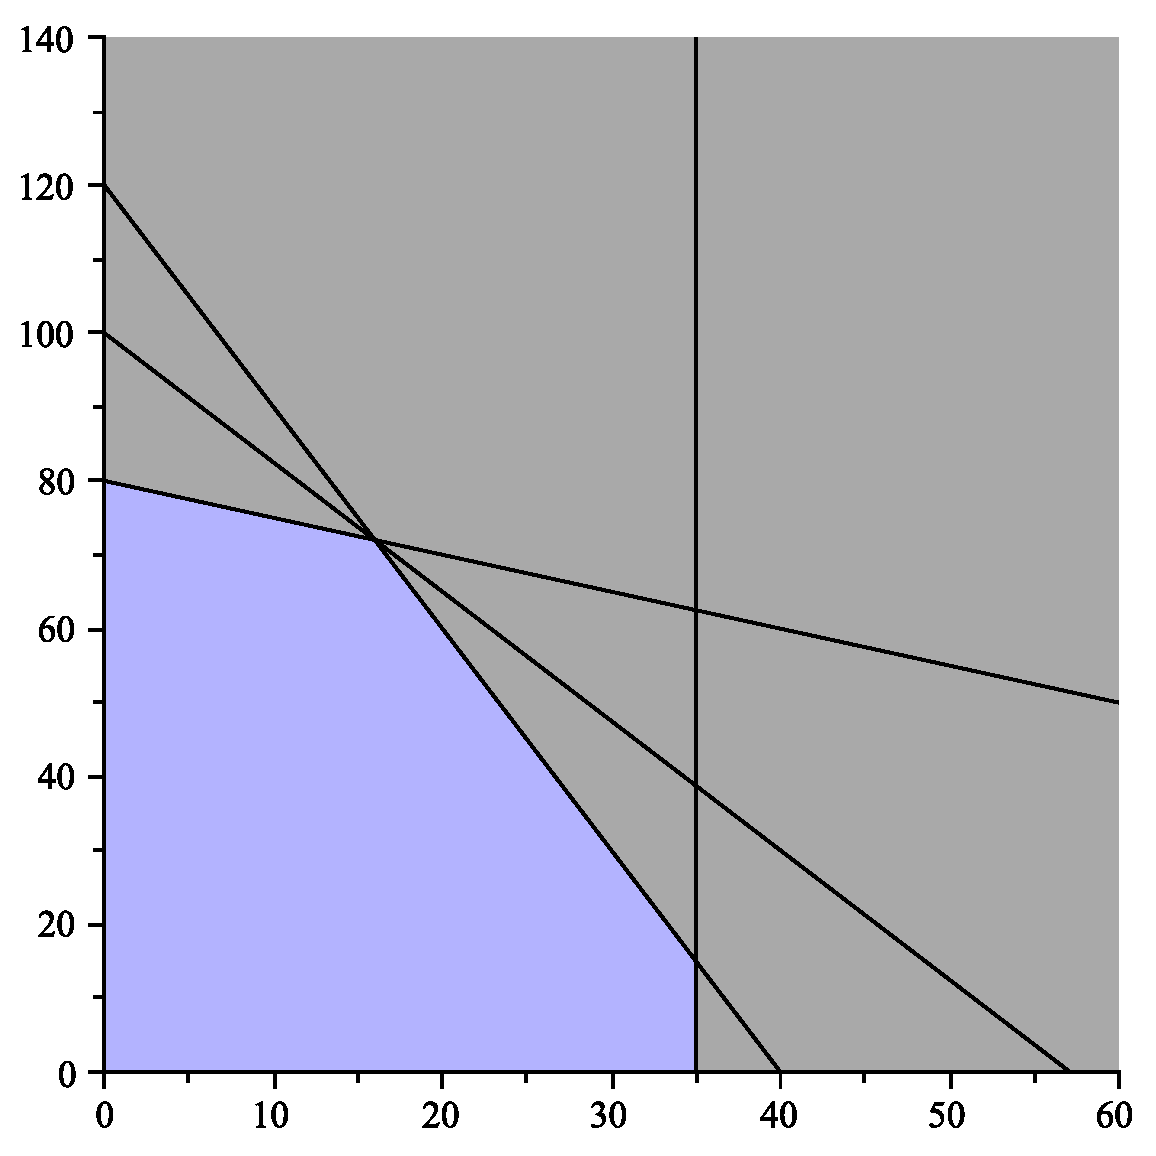
\includegraphics[scale=0.25]{DualDegeneracy1.pdf}}
\subfigure[RHS Decreased]{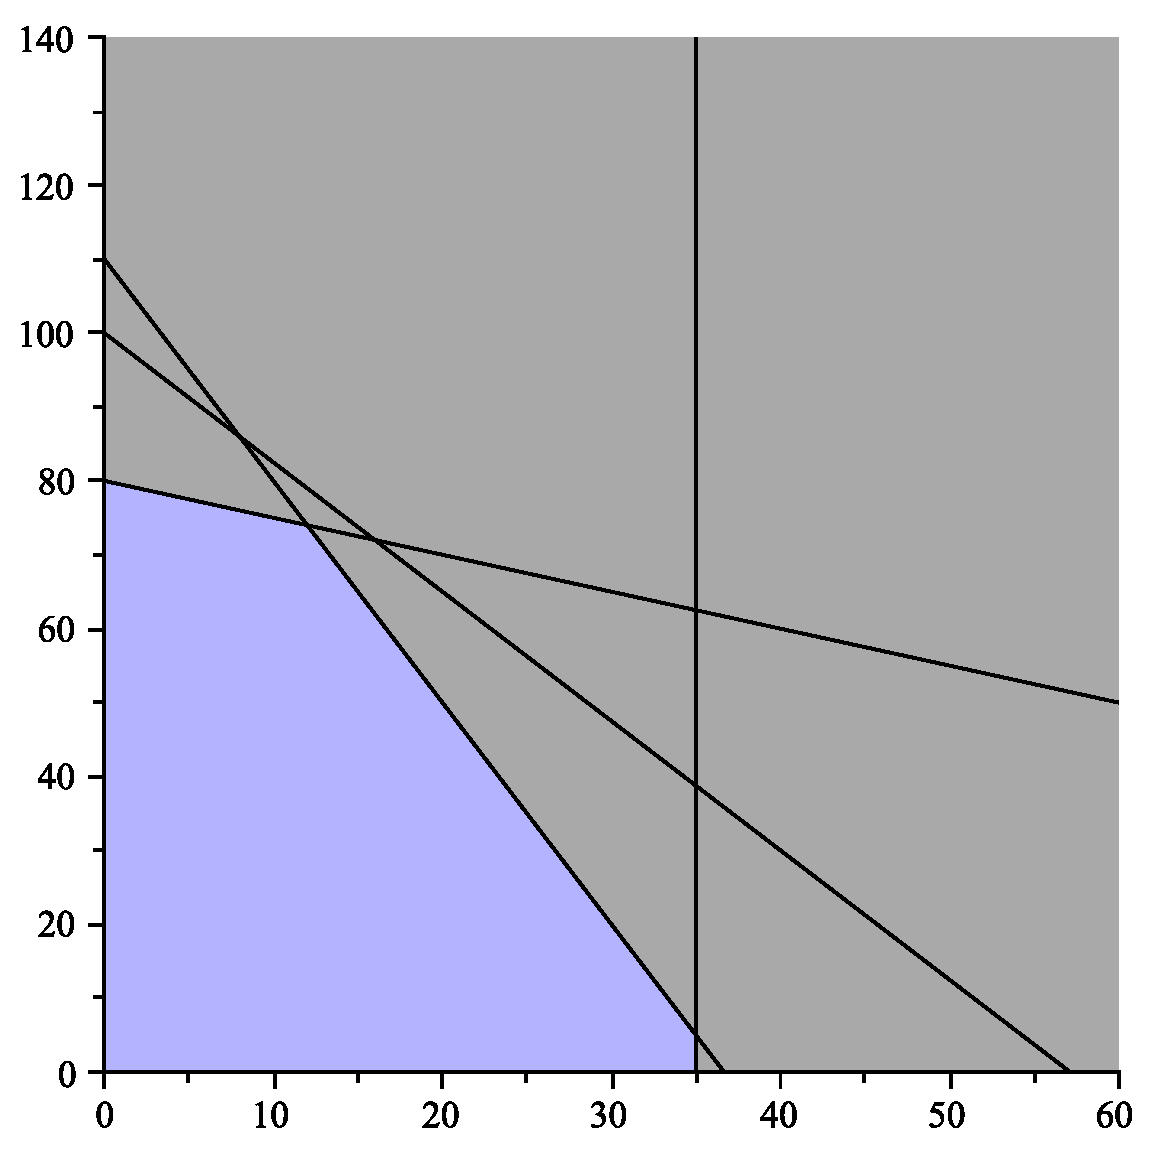
\includegraphics[scale=0.25]{DualDegeneracy2.pdf}}
\subfigure[RHS Increased]{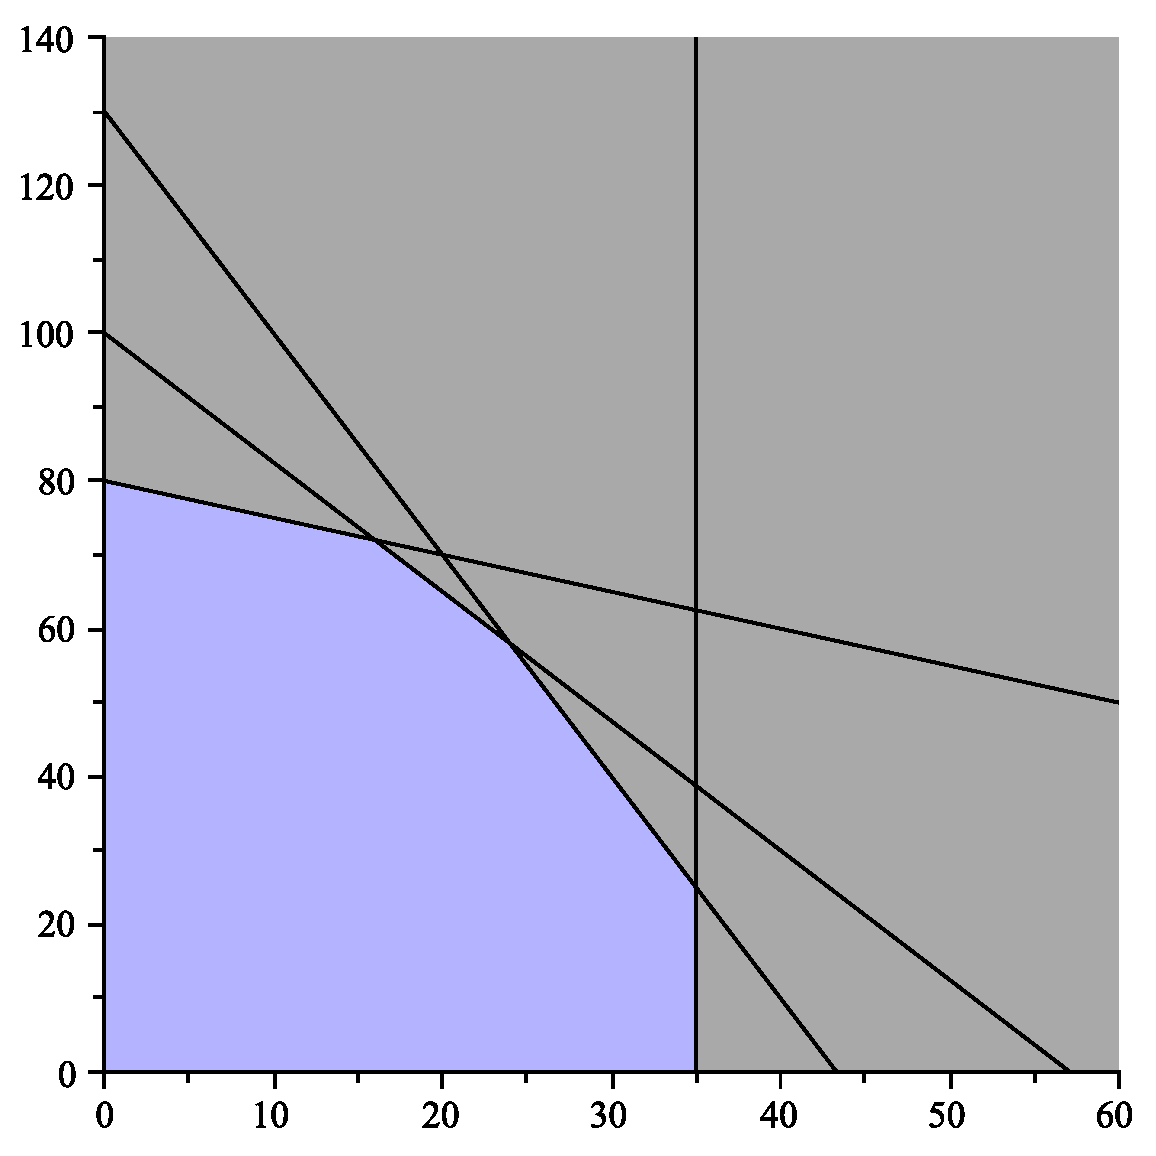
\includegraphics[scale=0.25]{DualDegeneracy3.pdf}}
\caption{Degeneracy in the primal problem causes alternative optimal solutions in the dual problem and destroys the direct relationship between the resource margin price that the dual variables represent in a non-degenerate problem.}
\label{fig:DegenDual}
\end{figure}

It should be noted that a true margin price can be computed, however this is outside the scope of the notes. The reader is referred to \cite{BJS04} (Chapter 6) for details.
\end{example}

\section{The Dual Simplex Method}
Occasionally when given a primal problem, it is easier to solve the dual problem and extract the information about the primal problem from the dual. 

\begin{example}
Consider the problem:
\begin{displaymath}
\begin{aligned}
\min\;\; & 	x_1 + 2x_2\\
s.t.\;\; &	x_1 + 2x_2 \geq 12\\
		 &	2x_1 + 3x_2 \geq 20\\
		 &	x_1, x_2 \geq 0
\end{aligned}
\end{displaymath}
To transform this problem to standard form, we would have to introduce surplus variables to obtain:
\begin{displaymath}
\begin{aligned}
\min\;\; & 	x_1 + 2x_2\\
s.t.\;\; &	x_1 + 2x_2 - s_1 = 12\\
		 &	2x_1 + 3x_2 - s_2 = 20\\
		 &	x_1, x_2, s_1, s_2 \geq 0
\end{aligned}
\end{displaymath}
In this case there is no immediately obvious initial basic feasible solution and we would have to solve a Phase I problem. Consider the dual of the original maximization problem:
\begin{displaymath}
\begin{aligned}
\max\;\;&12 w_1 + 20w_2\\
s.t.\;\; & w_1 + 2w_2 \leq 1\\
& 2w_1 + 3w_2 \leq 1\\
& w_1,w_2 \geq 0
\end{aligned}
\end{displaymath}
This is a maximization problem whose standard form is given by:
\begin{displaymath}
\begin{aligned}
\max\;\;&12 w_1 + 20w_2\\
s.t.\;\; & w_1 + 2w_2 + v_1 = 1\\
& 2w_1 + 3w_2 + v_2 = 1\\
& w_1,w_2,v_1,v_2 \geq 0
\end{aligned}
\end{displaymath}
In this case, a reasonable initial basic feasible solution for the dual problem is to set $v_1 = v_2 = 1$ and $w_1 = w_2 = 0$ (i.e., $w_1$ and $w_2$ are non-basic variables) and proceed with the simplex algorithm from this point.
\label{ex:EasyDualProblem}
\end{example}

In cases like the one illustrated in Example \ref{ex:EasyDualProblem}, we can solve the dual problem directly in the simplex tableau of the primal problem instead of forming the dual problem and solving it as a primal problem in its own tableau. The resulting algorithm is called the \textit{dual simplex algorithm}. 

For the sake of space, we will provide the dual simplex algorithm for a maximization problem:
\begin{displaymath}
P \left\{
\begin{aligned}
\max\;\;&\mathbf{c}\mathbf{x}\\
s.t.\;\;& \mathbf{A}\mathbf{x} = \mathbf{b}\\
&\mathbf{x} \geq \mathbf{0}
\end{aligned}\right.
\end{displaymath}
We will then shown how to adjust the dual simplex algorithm for minimization problems.


\begin{algorithm}
\caption{The Matrix form of the Dual Simplex Algorithm}
\label{alg:DualSimplexMatrixForm}
\begin{center}
\begin{minipage}[t]{\textwidth-1em}
\underline{\textbf{Dual Simplex Algorithm in Algebraic Form}}
\begin{enumerate*}
\item Choose an initial basic solution $\mathbf{x}_B$ and corresponding basis matrix $\mathbf{B}$ so that $\mathbf{w}\mathbf{A}_{\cdot j} - c_j \geq 0$ for all $j \in \mathcal{J}$, where $\mathcal{J}$ is the set of non-basic variables and $\mathbf{w} = \mathbf{c}_\mathbf{B}\mathbf{B}^{-1}$. 

\item Construct a simplex tableau using this initial solution.

\item If $\overline{\mathbf{b}} = \mathbf{B}^{-1}\mathbf{b} \geq \mathbf{0}$, then an optimal solution has been achieved; STOP. Otherwise, the dual problem is feasible (since $z_j - c_j \geq 0$). GOTO STEP 4.

\item Choose a \textit{leaving variable} (row) $x_{\mathbf{B}_i} = \overline{\mathbf{b}}_i$ so that $\overline{\mathbf{b}}_i < 0$.

\item Choose the index of the entering variable (column) $x_j$ ($j \in \mathcal{J}$) using the following minimum ratio test:
\begin{displaymath}
\frac{z_j - c_j}{\overline{a}_{j_i}} = \min\left\{\frac{z_k - c_k}{|\overline{a}_{k_i}|}  : k \in \mathcal{J}, \overline{a}_{k_i} < 0\right\}
\end{displaymath}

\item If no entering variable can be selected ($\overline{a}_{k_i} \geq 0$ for all $k \in \mathcal{K}$) then the dual problem is unbounded and the primal problem is infeasible. STOP.

\item Using a standard simplex pivot, pivot on element $\overline{a}_{j_i}$, thus causing $\mathbf{x}_{\mathbf{B}_i}$ to become $0$ (and thus feasible) and causing $x_j$ to enter the basis. GOTO STEP 3.
\end{enumerate*}
\end{minipage}
\end{center}
\end{algorithm}

The pivoting step works because we choose the entering variable specifically so that the reduced costs will remain positive. Just as we chose the leaving variable in the standard simplex algorithm using a minimum ratio test to ensure that $\mathbf{B}^{-1}\mathbf{b}$ remains positive, here we use it to ensure that $z_j - c_j$ remains non-negative for all $j \in \mathcal{J}$ and thus we assure dual feasibility is maintained.

The convergence of the dual simplex algorithm is outside of the scope of this course. However, it suffices to understand that we are essentially solving the dual problem in the primal simplex tableau using the simplex algorithm applied to the dual problem. Therefore under appropriate cycle prevention rules, the dual simplex does in fact converge to the optimal (primal) solution. 

\begin{theorem} In the absence of degeneracy, or when using an appropriate cycling prevention rule, the dual simplex algorithm converges and is correct.
\end{theorem}

\begin{example}
Consider the following linear programming problem:
\begin{displaymath}
\begin{aligned}
\max\;\;& -x_1 - x_2\\
s.t.\;\; &2x_1 + x_2 \geq 4\\
&x_1 + 2x_2 \geq 2\\
&x_1 , x_2 \geq 0
\end{aligned}
\end{displaymath}

Then the standard form problem is given as:
\begin{displaymath}
\begin{aligned}
\max\;\;& -x_1 - x_2\\
s.t.\;\; &2x_1 + x_2 - s_1 = 4\\
&x_1 + 2x_2 - s_2 = 2\\
&x_1, x_2 \geq 0
\end{aligned}
\end{displaymath}
The coefficient matrix for this problem is:
\begin{displaymath}
\mathbf{A} = \begin{bmatrix}
2 & 1 & -1 & 0\\
1 & 2 & 0 & -1
\end{bmatrix}
\end{displaymath}
In standard form, there is no clearly good choice for a starting basic feasible solution. However, since this is a maximization problem and we know that $x_1,x_2 \geq 0$, we know that the objective function $-x_1 - x_2$ must be bounded above by $0$. A basic solution that yields this objective function value occurs when $s_1$ and $s_2$ are both non-basic and $x_1$ and $x_2$ are both non-basic. 

If we let 
\begin{displaymath}
\mathbf{B} = \begin{bmatrix}-1 & 0\\0 & -1\end{bmatrix}
\end{displaymath}
Then we obtain the infeasible solution:
\begin{displaymath}
\overline{\mathbf{b}} = \mathbf{B}^{-1}\mathbf{b} = 
\begin{bmatrix}-4 \\ -2\end{bmatrix}
\end{displaymath}

Likewise we have:
\begin{displaymath}
\mathbf{w} = \mathbf{c}_\mathbf{B}\mathbf{B}^{-1} = \begin{bmatrix}0&0\end{bmatrix}
\end{displaymath}
since both $s_1$ and $s_2$ do not appear in the objective function. 
We can compute the reduced costs in this case to obtain:
\begin{gather*}
z_1 - c_1 = \mathbf{w}\mathbf{A}_{\cdot 1} - c_1 = 1 \geq 0\\
z_2 - c_2 = \mathbf{w}\mathbf{A}_{\cdot 2} - c_2 = 1 \geq 0\\
z_3 - c_3 = \mathbf{w}\mathbf{A}_{\cdot 3} - c_3 = 0 \geq 0\\
z_4 - c_4 = \mathbf{w}\mathbf{A}_{\cdot 4} - c_4 = 0 \geq 0\\
\end{gather*}
Thus, the fact that $\mathbf{w} \geq \mathbf{0}$ and the fact that $z_j - c_j \geq 0$ for all $j$, shows us that we have a \textit{dual feasible solution} and based on our use of a basic solution, we know that complementary slackness is ensured. 

We can now set up our initial simplex tableau for the dual simplex algorithm. This is given by:
\begin{displaymath}
\begin{array}{c}
\\
z\\
s_1\\
s_2
\end{array}
\left[
\begin{array}{c|cccc|c}
z& x_1 & x_2 & s_1 & s_2 &\text{RHS}\\
\hline
1 & 1 & 1 & 0 & 0 & 0\\
\hline
0 & -2 & -1 & 1 & 0 & -4\\
0 & -1 & \fbox{-2} & 0 & 1 & -2
\end{array}\right]
\end{displaymath}
We can choose either $s_1$ or $s_2$ as a leaving variable. For the sake of argument, suppose we choose $s_2$, the variable that's most negative as the leaving variable. Then our entering variable is chosen by comparing:
\begin{gather*}
\frac{z_1 - c_1}{|\overline{\mathbf{a}}_{21}|} = \frac{1}{|-1|}\\
\frac{z_2 - c_2}{|\overline{\mathbf{a}}_{22}|} = \frac{1}{|-2|}\\
\end{gather*}
Clearly, $1/2 < 1$ and therefore, $x_2$ is our entering variable.
\begin{displaymath}
\begin{array}{c}
\\
z\\
s_1\\
x_2
\end{array}
\left[
\begin{array}{c|cccc|c}
z& x_1 & x_2 & s_1 & s_2 &\text{RHS}\\
\hline
1 & 1/2 & 0 & 0 & 1/2 & -1\\
\hline
0 & \fbox{-3/2}	& 0 	& 1 	& -1/2 	& -3\\
0 & 1/2 	& 1 	& 0 	& -1/2 	& 1
\end{array}\right]
\end{displaymath}
At this point, we see we have maintained dual feasibility, but we still do not have primal feasibility. We can therefore choose a new leaving variable ($s_1$) corresponding to the negative element in the RHS. The minimum ratio test shows that this time $x_1$ will enter and the final simplex tableau will be:
\begin{displaymath}
\begin{array}{c}
\\
z\\
x_1\\
x_2
\end{array}
\left[
\begin{array}{c|cccc|c}
z& x_1 & x_2 & s_1 & s_2 &\text{RHS}\\
\hline
1 & 0 & 0 & 1/3 & 1/3 & -2\\
\hline
0 & 1		& 0 	& -2/3 	& 1/3 	& 2\\
0 & 0 		& 1 	& 1/3 	& -2/3 	& 0
\end{array}\right]
\end{displaymath}
It's clear this is the optimal solution to the problem since we've achieved primal and dual feasibility and complementary slackness. It's also worth noting that this optimal solution is degenerate, since there is a zero in the right hand side. 
\end{example}

\begin{exercise} Prove that the minimum ratio test given in the dual simplex algorithm will maintain dual feasibility from one iteration of the simplex tableau to the next. [Hint: Prove that the reduced costs remain greater than or equal to zero, just as we proved that $\overline{\mathbf{b}}$ remains positive for the standard simplex algorithm.]
\end{exercise}
\backmatter
\bibliography{References.bib}
\bibliographystyle{amsalpha}
\end{document}
\end
